% Template to be used while publishing
% a scientific work (PhD Thesis etc.)
% at the EDOC-Server of HU-Berlin
%    developed 2003-2008 by
% AG Elektronisches Publizieren,
% Computer- und Medienservice,
% Humboldt-Universitaet zu Berlin
%    with friendly support of
% TeX-Stammtisch in Berlin

% $Revision: 19 $
% $HeadURL: svn+ssh://ryckojox@svn.cms.hu-berlin.de/svn/projects/epub/latex/hudiss/mustermann.tex $
% $Date: 2009-07-03 15:49:19 +0200 (ptk, 03 lip 2009) $
% $Author$
% $Id: mustermann.tex 19 2009-07-03 13:49:19Z ryckojox $

% Questions, comments, support:
%    edoc-latex@cms.hu-berlin.de

% Documentation and information about the conditions of a publication:
%    http://edoc.hu-berlin.de/e_autoren/latex

% Upload:
%    https://edoc.hu-berlin.de/cgi/dokupload/dokupload.cgi

\documentclass[openright,% 
chapterprefix=true, appendixprefix=true, %
bibliography=totoc,
listof=totoc,
index=totoc,
fleqn,
BCOR=10mm,
pagesize=auto,
%firstinits=true
]{scrbook}[2007/12/24]

% The following package is necessary.
% To change the default options of the packages, use the key=value interface.
% See the documentation for details.
% If you need to use any special characters or LaTeX-commands 
% within the options, use \hudisssetup{} after loading this package,
% otherwise they will NOT work correctly.
\usepackage[    
    % inputenc=utf8, % default - latin1
    fontset=lmodern, % other possible parameters: lmodern, times, palatino
    % natbib={}, %include to use the natbib-package
    % jurabib={}, %include to use the jurabib-package
    % apacite={}, %include to use the apacite-package  
    hints=false, % set to 'false' for submission
    checktabu=false, % set to 'false' for submission
    draft=false, % set to 'false' for submission
    qserie=false
 ]{hudiss}

\hudisssetup{%
    titlepagefont={\Large\sffamily} % Use to change the titlepage font
}

% Fill out all the metadata here:
\hudissmetadata{%
    authorprefix={}, % e.g. Dipl.-Inf.
    authorfirstname={Jakob J.}, % first name
    authorsurname={Kolb}, % surname
    %authorsuffix={ }, % e.g. Ph.D.
    %authoradd={geboren am 22. April 1983 in Engelskirchen}, % date and place of birth
    doctitle={Heuristic Decision Making in World Earth Models}, % title of the thesis
    docsubtitle={}, % subtitle of the thesis
    docsubject={Statistical Physics}, % subject of the thesis (used in the properties of the pdf-document)
    approvala={
      Prof. Dr. Dr. h.c. mult. J\"{u}rgen Kurths
  }, % approvals: a-e
  approvalb={
    JProf. Dr. Ricarda Winkelmann
  },
  approvalc={
    Matthew Ives, PhD
  },
    % approvald={},
    % approvale={},
    degree={\so{doctor rerum naturalium} \\ (Dr. rer. nat.)}, % e.g. Dr. Rer. Nat.
    subject={Physik}, % e.g. Informatik
    specialization={Theoretische Physik},
    faculty={Mathematisch-Naturwissenschaftlichen Fakult\"at}, % in Dativ/Genitiv! e.g. Mathematisch-Naturwissenschaftlichen Fakult\"at II
    university={der Humboldt-Universit\"at zu Berlin}, % e.g. Humboldt-Universit\"at zu Berlin
    dean={Prof. Dr. Elmar Kulke}, % dean of the faculty
    president={Prof. Dr.-Ing. Dr. Sabine Kunst}, % president of the university
    datesubmitted={...}, % the date of the submission
    dateexam={Dienstag, 8. September 2020}, % the date of your last exam
    keywordsen={Statistical Physics, Complexity Economics, Agent-Based Modelling, Heuristic Decision Making}, % english keywords comma separated
    keywordsde={...} % german keywords comma separated
}

% If you wish to load any further packages, 
% make any own adjustments (e. g. for the package fancyhdr)
% or define any own commands
% put ALL of them in the following file:
%  Import packages
\usepackage{epigraph} 		% Allows to add nice quotations at the beginning of chapters
\usepackage{amsmath}		% mathematische Erweiterung, u.a. fr den align-environment
\usepackage{amsfonts}		% fr mathematische Symbole wie \mathbb{R}
\usepackage{amssymb}
\usepackage{amsthm}
\usepackage{multirow}
\usepackage{enumerate}
%\usepackage{sidecap}
\usepackage[section]{placeins}
\usepackage{booktabs}
\usepackage{lscape}
\usepackage{longtable}
\usepackage{
  empheq, % for boxes around equations
        wrapfig, % for wrapped figures in text
        makecell, % for custom formatting in table cells
        hhline, % for custom hlines in tables
        tablefootnote, %for footnotes in tables
        wrapfig, % for figures wrapped in text
        cleveref % for better references
}
\usepackage{makeidx} 		% Create index
\makeindex

\usepackage{chngcntr}		% Make footnote counting continuous throughout the whole document
\counterwithout{footnote}{chapter}

%\usepackage[a-1b]{pdfx}  % Allow compliance with PDF/A standard
\usepackage[sort&compress]{natbib}

\iffalse
%
%  Define custom citation style including paper numbers
%
\usepackage[style=authoryear,maxcitenames=2,maxbibnames=100,natbib=true]{biblatex}
%\usepackage[backend=bibtex,style=authoryear,maxcitenames=2,maxbibnames=100,natbib=true, url=false]{biblatex}

\newbibmacro*{papernum}{%
  \iffieldundef{usera}{%
  }{%
    \addcomma\space
    \printfield{usera}%
  }%
}

\DeclareFieldFormat{labelyear}{%
  \stripzeros{#1}%
  \iffieldundef{extrayear}{%
    \usebibmacro{papernum}%
  }{%
  }%
}

\DeclareFieldFormat{extrayear}{%
  \iffieldnums{labelyear}
    {\mknumalph{#1}\usebibmacro{papernum}}
    {\mkbibparens{\mknumalph{#1}\usebibmacro{papernum}}}}

\addbibresource{bibliography.bib}
%%%
\fi

% easy column vectors
\newcount\colveccount
\newcommand*\colvec[1]{
        \global\colveccount#1
        \begin{pmatrix}
        \colvecnext
}
\def\colvecnext#1{
        #1
        \global\advance\colveccount-1
        \ifnum\colveccount>0
                \\
                \expandafter\colvecnext
        \else
                \end{pmatrix}
        \fi
}
 
\raggedbottom 				% Change page layout style
\allowdisplaybreaks[2]		% Allow page breaks in "align" environment

% Hurenkinder und Schusterjungen verhindern
\clubpenalty9999
\widowpenalty9999
\displaywidowpenalty9999

\usepackage{microtype}
\usepackage{hfoldsty}
\usepackage{ellipsis}
\usepackage{nicefrac}

%  Settings
\setlength{\epigraphrule}{0pt}				%  Remove epigraph rule
\setlength{\epigraphwidth}{0.50\textwidth}		%  Change epigraph width
\setlength{\mathindent}{0pt}				%  Set indent of equations
\setcounter{tocdepth}{1}					%  Set table of contents depth
\setkomafont{caption}{\sffamily\small}
\setkomafont{captionlabel}{\sffamily\bfseries\small}
\renewcommand*{\partpagestyle}{empty}

%  Definitions
\newtheorem{mydef}{Definition}	[chapter]			%  Define customized theorem environment
\newcommand{\nn}[1]{{\it #1*}}				%  Define customized style for index entries

%  Environments
\newenvironment{mytabular}{%				%  Custom tabular environment with sans-serif font
  \sffamily \small
  \tabular
}{%
  \endtabular
}

%  Set preambles

%  Set index preamble
%\setindexpreamble{All page numbers in \textit{italics} (additionally marked by asterisks *) are references to the definitions of the respective terms. In contrast, evenly typeset page numbers refer to further usage of the expressions.
%\par\bigskip}

%  Citation aliases
%\defcitealias{Donges2012b}{Donges et al., in prep., P1} % PRE
%\defcitealias{Wiedermann2012}{Wiedermann et al., in prep., P2} % EPL
%\defcitealias{Feldhoff2012b}{Feldhoff et al., in prep., P3} % EPL
%\defcitealias{Feldhoff2012a}{Feldhoff et al., subm., P4} % PLA
%\defcitealias{Radebach2012}{Radebach et al., subm., P5} % PRE
%\defcitealias{Zou2011}{Zou et al., in press, P6} % EPL
%\defcitealias{Donner2012}{Donner and Donges, 2012, P7} % Acta Geophysica
%\defcitealias{Donges2012}{Donges et al., 2012, P8} % PRE
%\defcitealias{Heitzig2010}{Heitzig et al., 2012, P9} % EPJ B
%\defcitealias{Donges2011c}{Donges et al., 2011b, P10} % PNAS
%\defcitealias{Donges2011b}{Donges et al., 2011a, P11} % NPG
%\defcitealias{Tominski2011}{Tominski et al., 2011, P12} % Viz Conference, London
%\defcitealias{Donner2011a}{Donner et al., 2011b, P13} % IJBC
%\defcitealias{Donges2011a}{Donges et al., 2011c, P14} % EPJ B
%\defcitealias{Donner2011b}{Donner et al., 2011a, P15} % EPJ B
%\defcitealias{Zou2011b}{Zou et al., 2011, P16} % Complex Systems and Complexity Science
%\defcitealias{Zou2010}{Zou et al., 2010, P17} % Chaos
%\defcitealias{Donner2010a}{Donner et al., 2010b, P18} % PRE(R)
%\defcitealias{Donner2010b}{Donner et al., 2010c, P19} % NJP
%\defcitealias{Marwan2009}{Marwan et al., 2009, P20} % PLA
%\defcitealias{Donges2009b}{Donges et al., 2009b, P21} % EPL
%\defcitealias{Donges2009a}{Donges et al., 2009a, P22} % EPJ ST
%
%\defcitealias{Donner2012b}{Donner and Donges, subm., C1} % NOLTA 2012
%\defcitealias{Marwan2010b}{Marwan et al., 2010a, C2} % NOLTA 2010
%\defcitealias{Donner2010d}{Donner et al., 2010a, C3} % NOLTA 2010


% The order of the parts in the document is only our suggestion,
% you can change it, if you wish.
% Don't put any other text between those commands.
% Do not remove the \*matter macros.
% Use standard macros to include new chapters.

\begin{document}
    \frontmatter
        \maketitle
        \cleardoublepage

\null\vfill\itshape

\begin{flushright}
	
\end{flushright}
\thispagestyle{empty}
\upshape\cleardoublepage


        \selectlanguage{english}

\begin{abstract}
...

\end{abstract}

\cleardoublepage

\selectlanguage{ngerman}
\begin{abstract}
...

\end{abstract}

\cleardoublepage

\selectlanguage{english} % Switch back to English to obtain the corrected heading for table of contents

        
%\renewcommand{\thechapter}{\hspace{-0.45cm}}
\addcontentsline{toc}{chapter}{Acknowledgements}
\chapter*{Acknowledgements}
\begin{minipage}[t][0pt]{\linewidth}

Many individuals and organizations enabled and supported me in writing this thesis.\\

 First of all, I thank Prof. J\"{u}rgen Kurths for the continuous trust and support during the last four years and for hosting me at the Potsdam Institute for Climate Impact Research (PIK). Special thanks go to Jobst Heitzig for day-to-day supervision, for numerous discussions, for plenty of freedom when I needed it and for guidance and holding me accountable when I wanted it.
 I want to thank Ricarda Winkelmann and Jean-Denis Mathias for their willingness to critically evaluate this thesis.
 Many thanks to my colleagues and Friends especially Jonathan Donges, Reik Donner, Marc Wiedermann, Wolfram Barfuss and Benjamin Maier, I much appreciated your extensive comments and feedback on my work in various stages. I want to thank them and all of my other colleagues at the COPAN flagship project also for their input and shared experiences in scientific life and work over the last four years.
 Also, I am deeply indebted to my coauthors, especially Finn M\"{u}ller-Hansen, and Doyne Farmer from whom I have learned a great deal about the strengths and weaknesses of economic models, Yuki Asano, who is one of the most industrious persons that I have met in my life and who constantly pushed us to do better, faster and Maurits Ertsen with whom, during long calls on the phone, I had the most interesting discussions on the meaning of modelling and its limits as an ontological tool.\\


 I am much obliged to the Foundation of German Industries (SDW) for placing their trust in me in the early phase of this project. Their scholarship was so much more than just financial support. I also want to thank the Princeton-Humboldt Cooperation and Collective Cognition Network (CoCCoN), and there within especially Pawel Romanczuk, for the opportunity to participate and providing the funds to repeatedly visit Princeton University.
 I am also grateful for all of those who provided me with library and technical infrastructure especially the European Regional Development Fund (ERDF), the German Federal Ministry of Education and Research and the Land Brandenburg for enabling my work by providing resources on the high performance computer systems at PIK.\\

 I am vary grateful to Winnie Poel for many things but at this point especially for her continued support and the big parts of our shared reproductive labor that she took on during the final stages of writing this thesis.
And last but not least, I feel blessed for my two wonderful daughters who came into my life during the work on this thesis and who never get tired of reminding me that there is plenty of life outside of research.
\end{minipage}

        \tableofcontents
        \listoffigures
        \listoftables
        \selectlanguage{english}

%\renewcommand{\thechapter}{\hspace{-0.45cm}}
\addcontentsline{toc}{chapter}{List of Publications}
\chapter*{List of Publications}

This dissertation is partly based on the following publications. The identifiers, \textit{e.g.}, P1, given below are cited in the text to highlight passages that are connected to one or more of these papers.

\paragraph{Papers}
\begin{enumerate}[P1]
    \item \bibentry{Kolb2019b}
    \item \bibentry{Mueller-Hansen2017}
    \item \bibentry{Donges2018}
    \item \bibentry{Asano2019}
    \item \bibentry{Kolb2019a}

\end{enumerate}

%\paragraph{Conference proceedings}
%\begin{enumerate}[C1]
%\item ...
%
%\end{enumerate}

    \mainmatter
        %%\renewcommand{\thechapter}{\hspace{-0.45cm}}
\addcontentsline{toc}{chapter}{List of frequently used mathematical symbols}
\chapter*{List of frequently used mathematical symbols}

\begin{tabular}{ll}
...

\end{tabular}


        \chapter{Prologue: Learning from the Rise and Fall of the Ancient Maya}
\label{chapter:maya}
This chapter is based on unpublished work. However, a publication [P1] together with Maurits Ertsen, Jonathan Donges and Reik Donner is in preparation.
\section{Introduction}

% Geosimulations as one approach to understand geological realities.
Archeologists and historians try to understand archeological, geographical and geological records in terms of rulesets that explain the processes underlying the historical environmental conditions and societies that produced them.
Geosimulations are one way to implement and test such sets of rules by combining them with geographical and geological data, analyzing their results and inter-comparing them with the empirical findings. This strategy has proven useful especially for more complex sets of rules, where the impacts of changes in individual assumptions or parameters are difficult to track by logical reasoning alone. \textcolor{red}{[CITE SOME OF MAURITS WORK HERE]}

% the epistemological dimension of modelling
However, the design and calibration of such models heavily relies on empirical data, as well as reasonable assumptions about processes and storylines that can guide the analysis of the model. Based on these assumptions and the data at hand, a modeler usually defines the different parts of a model as agents that behave according to local rules that prescribe different actions for them depending on the current state of their environment and/or the actions of other agents. This raises the question, how the modeler can avoid to structure the agents in a model (in terms of equations, algorithmic rules and parametrization) to an extent that prevents the model from generating insights that go beyond the data, process models and storylines that went into the model construction in the first place.

From a conceptual perspective, the individual agent in such a model cannot show new (in the sense of autonomous) types of behavior anyway, since all its actions are fully determined by the prescribed set of rules. Even if these rules were involving some element of randomness, the modeller still had to specify this randomness with respect to its statistical properties. 

% agent-based models as a way out through emergent dynamical properties.
Yet, this does not mean that investigating the behavior of individual agents is not interesting. At the same time, many studies with agent-based models (ABMs) have illustrated, how at the system level various surprising effects can emerge from the interactions of many agents with individually well predictable behaviors \citep{Epstein1999}. \footnote{I use here a weak notion of emergence, which allows explaining macroscopic (global) phenomena on the basis of microscopic (local) interactions of the system's constituents that differ from the explained macro-phenomena. This is opposed to strong emergence, that embraces the irreducibility of macro-phenomena to lower-level dynamics. For a corresponding discussion, see \citet{Bedau1997}.} 

%Especially in the physics and complex systems science community, the possibility of emergent phenomena has sparked considerable interest. A variety of methods inspired from a physical context (such as aggregation methods and stability and bifurcation analysis) have been applied to various different ABMs to gain better understanding of their emergent dynamical properties. This general approach has found important applications in various fields, such as ecology \citep{Grimm2005}, business \citep{Bonabeau2002}, sociology \citep{Macy2002} and economics \citep{Tesfatsion2006, Hamill2016}.

A particularly interesting application of ABMs in the field of archeological research is the case of the ancient Maya civilization on the Yucatan peninsula and nearby regions of Central America. The rise and fall of the ancient Maya society has been debated as an iconic example for the catastrophic decline and reorganization of a complex social-ecological system. 
Paleoclimate records show that coincidentally with the major societal changes of the Maya civilization, there have been a number of severe drought episodes in the region \cite{Evans2018}.
Different studies argue that these changing climatic conditions could have been the main driver of this decline \citep{Medina-Elizalde2012, Kennett2012}. Others argue, however, that rather than a single cause, there must have been a number of different causal factors \citep{Masson2012} such as political instability and warfare as well as a shift from land to sea-borne trade.

A number of different models have been employed for studying the interaction of the Maya population with their surrounding forest ecosystem as well as other resources such as freshwater and the influence of climatic conditions \citep{Heckbert2013,Turner2012a, ertsen2018}. The present study will build upon one the those models, the agent-based MayaSim model originally developed by Heckbert \citep{Heckbert2013, Heckbert2013model}. This model has been previously used to support the hypothesis that the decline of the ancient Maya civilisation was first and foremost caused by deteriorating climatic conditions, which had been modeled through declining mean annual precipitation.

This chapter covers a re-implementation of the MayaSim model that addresses some problems of the original model version. I analyze the model with respect to its sensitivity to key parameters and evaluate the response of the model dynamics to drought events of variable strength and severity. I find that in different parameter regimes, the model exhibits different emergent dynamical properties. Specifically, the model transitions from A) a regime where the population gets gradually extinct over B) a regime of cyclic dynamics with predator--prey like dynamics between the Maya agriculture and the forest ecosystem to C) a regime with a large sustained population, a large static trade network between individual Maya settlements and a deteriorated state of the ecosystem. Most importantly, I find that with realistic parameter values, the model response to drought events does not support the hypothesis of changing climatic conditions as a sole driver for the deterioration of the ancient Maya civilization.

\section{Model Description}

%Explanation of the model I used, referring to figure \ref{fig:model_snapshot} stating the parallels to and deviations from the original Heckberth model.

\begin{figure}
    \centering
    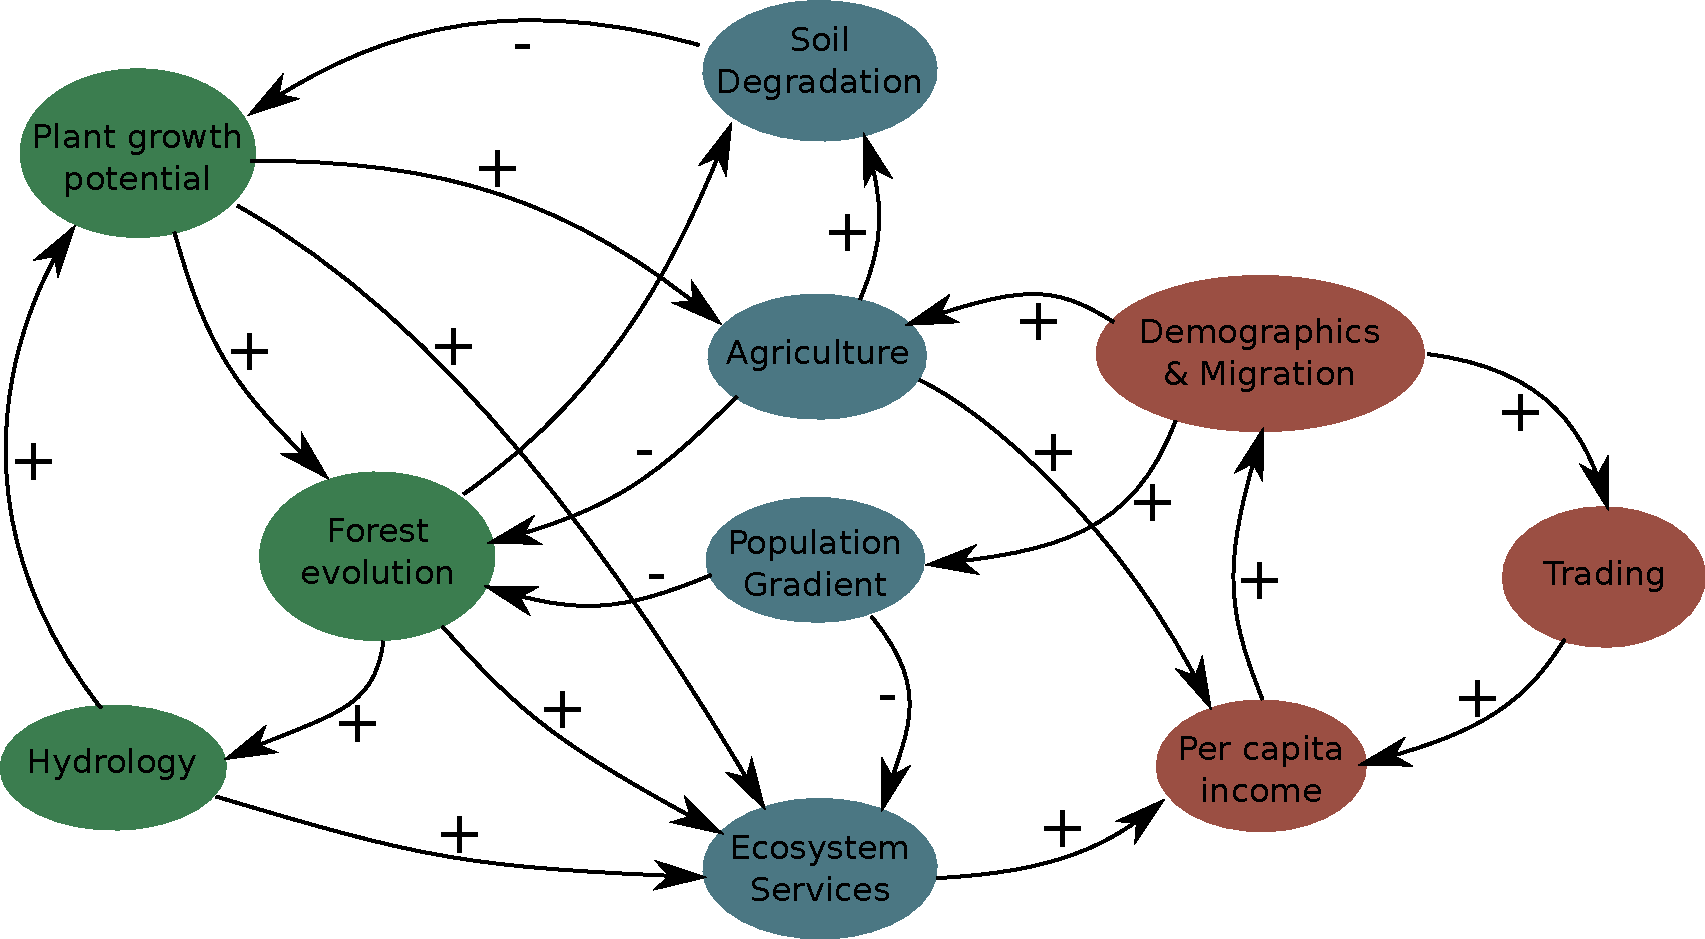
\includegraphics[width=.9 \textwidth]{figures/model_flowchart.pdf}
    \caption{\textbf{Simplified flowchart of the MayaSim model.} Arrows indicate feedbacks between different processes, colors indicate different subsystems namely green for the ecosystem, red for the socio-economic system and blue for processes that interface between the two aforementioned.}
    \label{fig:my_label}
\end{figure}

The MayaSim Model is described in detail by \cite{Heckbert2013}. It represents settlements as agents on a gridded landscape that is used to model the surrounding ecosystem. The ecosystem is described by precipitation, hydrology, agricultural productivity and forest succession, it provides ecosystem services for the Maya population and drives regeneration of soils that have been eroded due to agriculture.

% Ecosystem Processes
\begin{itemize}
    \item \textbf{Precipitation} is driven by empirical data from \cite{Hijmans2005} and varied to mimic paleoclimatic conditions as presented in \cite{Prufer2011}.
    \item \textbf{Hydrology} is modelled by a cellular automata model for surface water flow on the geological elevation profile. For the precipitation on each cell, the water is partly infiltrated and partly moves as water flow along the gradient of surface elevation (also considering the standing water [mm] already at that location) to a neighboring cell. This process is repeated iteratively such that a steady state flow and lake profile forms. 
    \item \textbf{Net primary productivity} is a function of precipitation and temperature as given by the Miamy model in \cite{Lieth1975}.
    \item \textbf{Agricultural productivity} is calculated as with a linear additive model from net primary productivity, soil productivity, surface water flow, and soil degradation.
    \item \textbf{Forest succession} is represented by a cellular automata model where the state of a cell depends on its own history and the state of its neighboring cells. A cell can be in three different states that represent cleared/cropped land, secondary regrowth and climax forest referred to as state 1, 2, and 3 respectively. Forest cells at a small constant rate representing natural disturbance. This rate is linearly amplified by the population density of nearby settlement to represent wood harvesting. The state of a forest cell increases after a certain number of time steps without disturbance to the next higher state where for the increase to state 3 at least three neighboring cells have to be in this state already representing the need to have local vegetation for seed dispersal.
	\item \textbf{Ecosystem Services} are modeled by quantifying the availability of provisioning services of arable soils, fresh water and access to timber as well as food from the forest ecosystem.
\end{itemize}


The socio-economic system of the Maya population is described by settlement nodes with a certain population that generate their per capita income from agriculture, usage of ecosystem services and trading with other settlements. 

% Socio-economic processes
\begin{itemize}
	\item \textbf{Agriculture} drives soil erosion and the clearing of forest where the latter is additionally intensified by the presence of people in the forest using ecosystem services. 
	\item \textbf{Trade} is described by network of trade relations between settlements where settlements above a certain size form trade relationships with their closest neighbors, preferably with those with higher population. Income from trade depends on the total size of the trade network, the possition in the trade network as well as the travel cost to neighboring settlements.
	\item \textbf{Population growth} is described in a simple malthusian fashion with a fixed birth rate and a death rate inversely proportional to per capita income.
	\item \textbf{Migration}: The willingness of people to migrate is driven by low per capita income in existing settlements. If the size of the fraction of the population that exceeds a certain size, it leaves the settlement and tries to establish a new settlement. For the location of their new settlement they sample available locations and maximize their utility depending on available ecosystem services and travel cost depending on distance from the settlement of origin.
\end{itemize}
For detailed description of the above processes, calibration of the model and parameter values please refer to \cite{Heckbert2013} and \cite{Heckbert2013model}

\begin{figure}[!t]
\centering
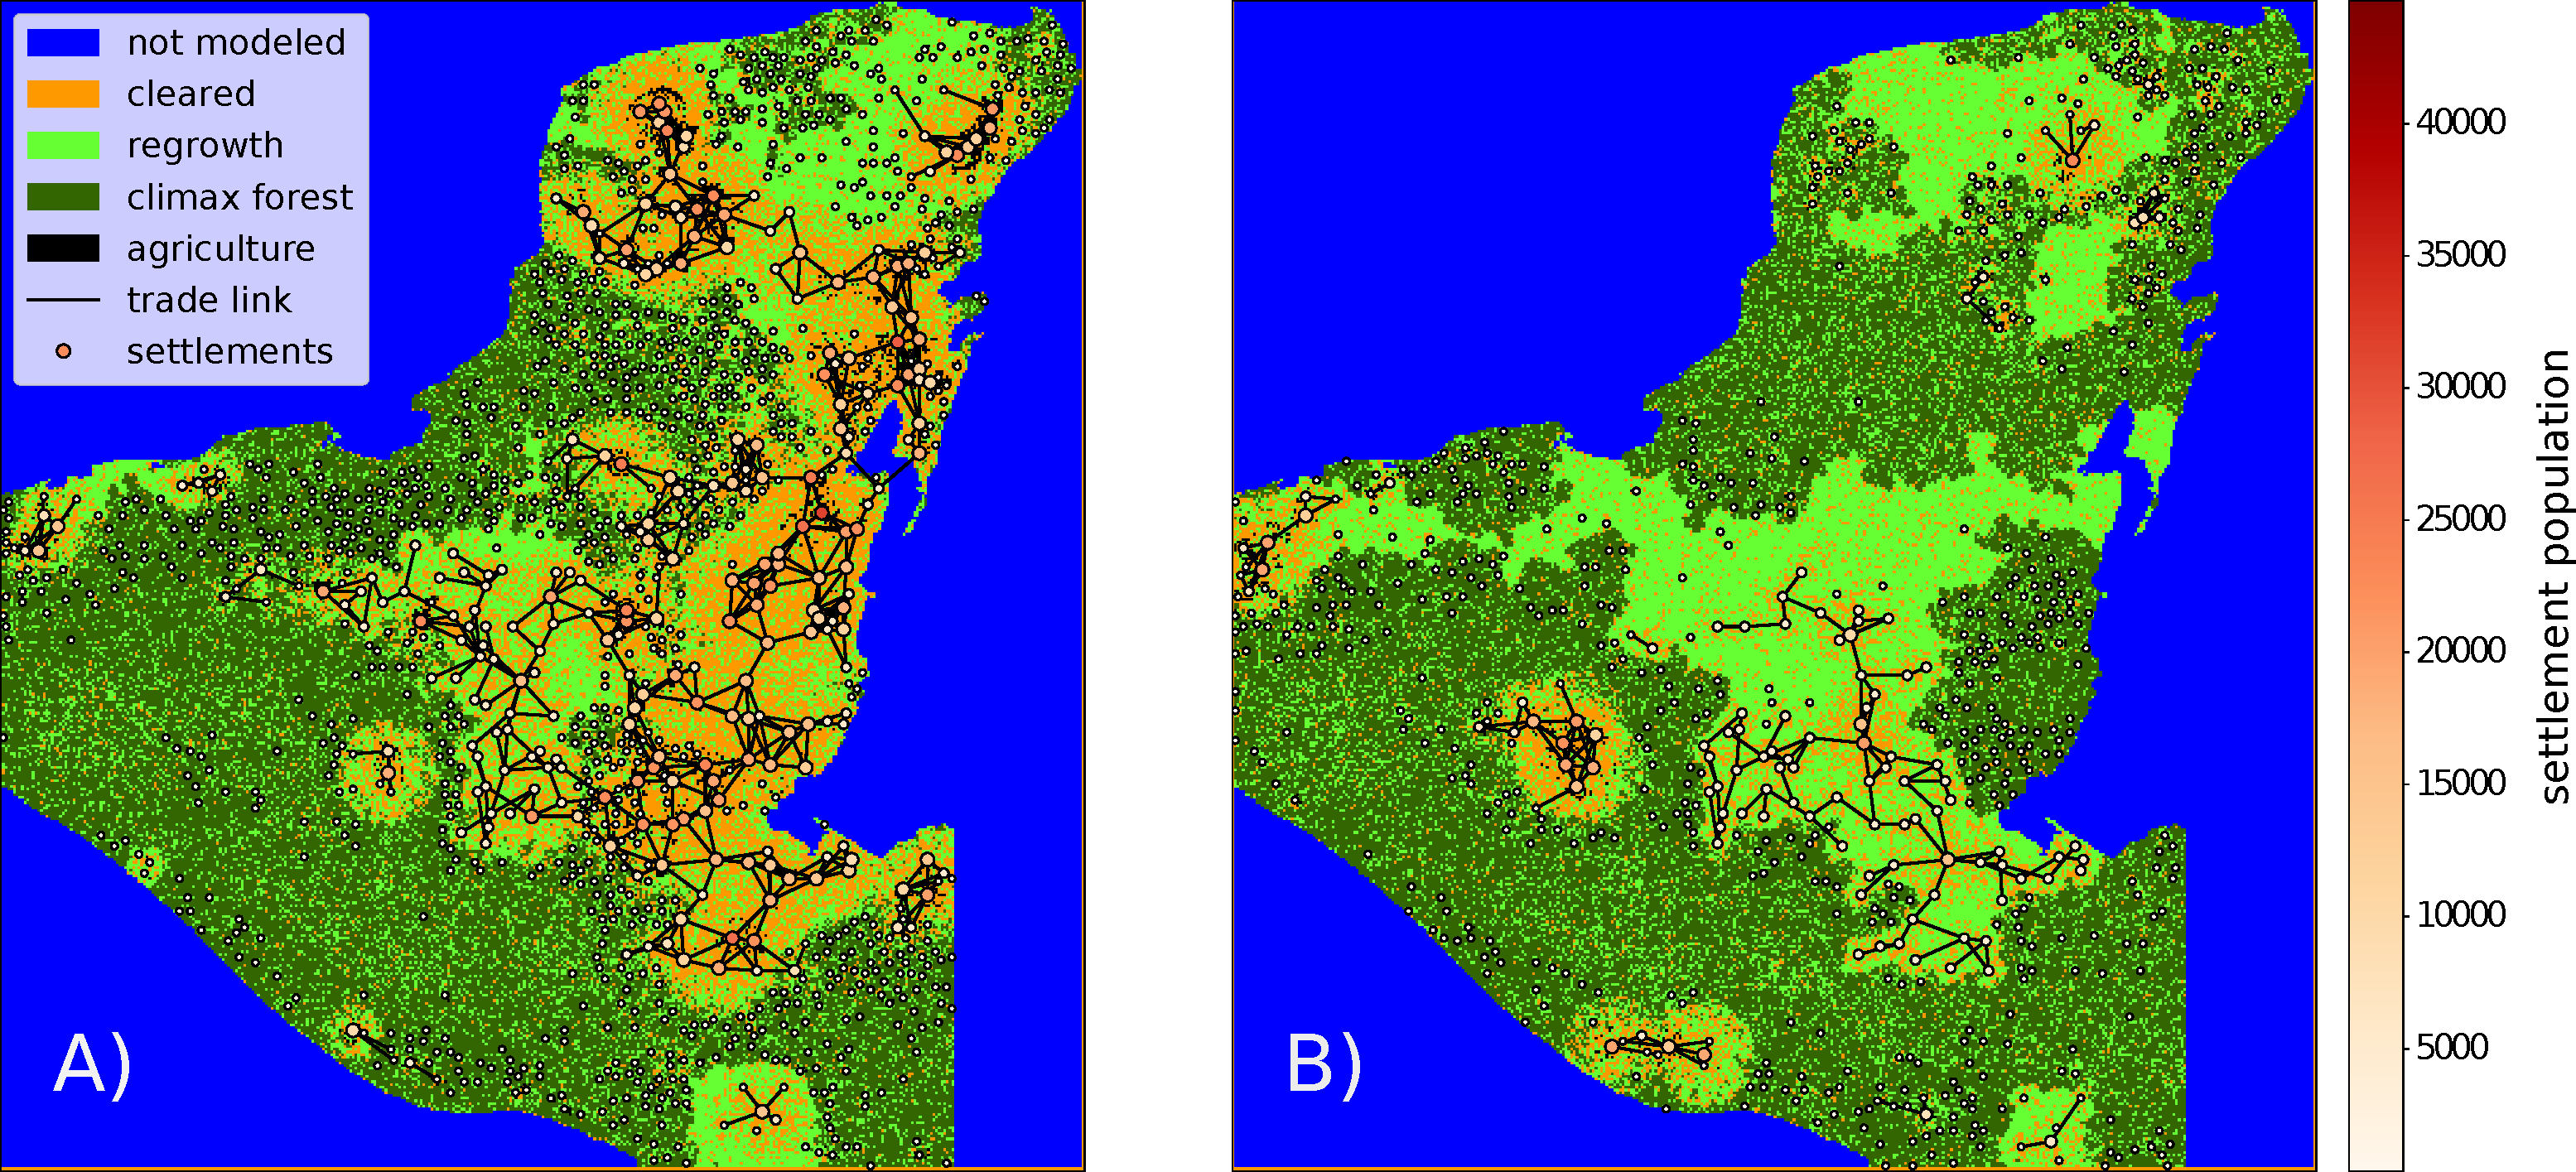
\includegraphics[width=\textwidth]{figures/map_plots.pdf}
\caption{\textbf{Simulation snapshots} showing a complex society in panel A) and a degraded society state in pannel B). Different shades of green indicate different ecosystem states: Black indicates agricultural usage, brown indicates wasteland, light green indicates secondary regrowth, and dark green indicates climax forest. The nodes of the network are settlements with the fill color indicating their population size and the links showing trade relations between them. The brightened area around settlements shows the area that is affected by the settlements usage of ecosystem services. The two different states are taken from the same model run 280 years appart.}
\label{fig:model_snapshot}
\end{figure}

I deviate from the original model in one aspect that I outline and motivate in the following.
In the original model, each settlement needs to use at least one cell for agriculture else it is deleted and its population is assumed to die. I release this constraint as larger settlements are part of a trade network and can trade agricultural produce from other settlements and smaller settlements can get by from income from ecosystem services. I understand that the original version was motivated by the assumption that every settlement must produce some food for its inhabitants, yet this resulted in situations where very large cities rely on the agricultural produce of one cell. Also it neglects the fact that agricultural produce can be traded against products from larger cities' more specialized economies as suggested by \cite{Dahlin2007} as well as the fact that large cities usually had power over smaller settlements in their surroundings and were able to collect tribute from them.

There are some discrepancies between the reference implementation of the model \cite{Heckbert2013model} and the model description paper \cite{Heckbert2013}. In the following processes, our implementation deviates from the reference implementation to be in line with the model description paper: 

\begin{itemize}
    \item In the reference implementation income from agriculture and ecosystem services are calculated as the mean income from cropped cells and cells under a settlements influence respectively. However the model description paper states that income should be calculated as the sum of the yields from cropped cells and cells under the settlements influence. I implemented the process according to the model description paper.
    \item In the reference implementation settlements are not deleted if their population falls below a threshold for subsistence. In our implementation they do.
    \item In the reference implementation settlements build trade relations with their neighboring settlements once their population exceeds a certain threshold. They do however not not lose trade links if their population falls below the respective threshold. In our implementation they do.
\end{itemize}

\section{Methods}
\textit{How can measures of resilience in complex systems be meaningfully applied to geo-simulations?}

% these are the concepts of resilience in complex systems
I use the concept of resilience \citep{Holling1973} aims to describe the response of a system to perturbations and changing environmental conditions. 


As such, it has been defined in two ways: 
first as \emph{engineering resilience} or \emph{persistence resilience} which describes the ability of a system to return to a particular equilibrium or steady-state after a perturbation \citep{Holling1973, Gunderson2000}, and
second, as \emph{transformation resilience} which means ``the capacity of a system to absorb disturbance and reorganize while undergoing change so as to still retain essentially the same function, structure, identity, and feedbacks'' \citep{Walker2004}.

% these concepts have been applied to ecological as well as social-ecological systems
%The concept of resilience has been used abundantly to describe the response of ecological systems to changing environmental conditions due to natural or antropogenic influences \citep{Holling1978, Ludwig1978, Regier1996, Walker1981, Westoby1989, Fiering1982, Walters1986} and more recently also to study SES under the same conditions \citep{Berkes1998, Berkes2003, Adger2000, Adger2005, Galaz2005}

% this is one concept that is used to measure them in social ecological systems
Since the state space of the Mayasim Model is very high dimensional (including the states of each forest cell as well as the positions and state variables of settlements as well as the configuration of the trade network between them), it would be very complicated and tedious to use a persistence resilience approach that measures the response of the full state of the system to changing environmental conditions. Especially because the full state of the model (as we will see later) is not necessarily an equilibrium state but can exhibit endogenous oscillations.
However, one can use a transformation resilience approach to classify the response of the model to exogenous shocks such as drought events.
To do this, one can classify the macroscopic dynamics of the model according to dynamical properties that signal the same function, structure, identity, and feedbacks on the microscopic level of the model. More precisely, in terms of aggregated model variables, one can classify different attractors in the models state space and test whether large perturbations move the model out of the basin of attraction of the desired part of the state space. The simple, one dimensional case of this is illustrated in fig. \ref{fig:basin_stability}.

% this is how I aim to adapt/apply it to geosimulations
Technically, I implement this as follows:
I study the MayaSim model in terms of macroscopic properties and find that it exhibits at least one attractor and one absorbing boundary. The absorbing boundary being zero population from where (due to non existent in-migration into the model space) there is no coming back, the attractor is a complex society state that is subject to a phase transition like event for rising possible income from trade changing from a repeating pattern of development, decline and spatial reorganization to a steady, high population state characterized by a complex trade network between settlements and a degraded ecosystem.

Given these macroscopic dynamical properties of the model, I measure transformation resilience as follows: First I let the system develop until it reaches the complex society attractor. Second, I let the system undergo perturbations of different strength and duration (I reduce the mean annual precipitation for a given percentage over a given period of time). Third, after the perturbation, I measure whether the system returns to the attractor - representing a similar macroscopic state and system functionality with a transformed microscopic configuration - or whether it runs off into the absorbing state with zero population.

Finally, I compare the magnitude of drought events that is sufficient to drive the system into the zero population absorbing state with drought events that can be motivated with empirical data from paleo-climatic records.

\begin{figure}[!t]
\centering
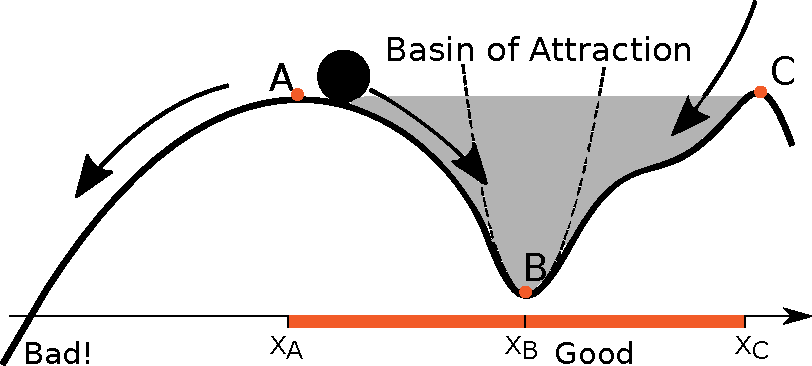
\includegraphics[width=0.5\textwidth]{figures/Basin_Stability.pdf}
\caption{\textbf{Illustration of the concept of resilience/stability}. Imagine a projection of the state space of the system onto a one dimensional manyfold lateral to an attractor or a stable manyfold indicated by B. Then, if the state of the system is in the basin of attraction of B (indicated in grey) its inherent dynamic will eventually return its state back to the stable manyfold. However, if the system is moved sufficiently far away from B (past points A or C) through e.g. a large scale perturbation, it will not return to its previous state, but will move towards an entirely different state space region. Note that for the MayaSim system, this observation holds in terms of macroscopic variables only. After a perturbation, even if the system returns to its previous state in terms of macroscopic variables, its microscopic configuration in terms of geography, demography and ecosystems state can be changed dramatically.}
\label{fig:basin_stability}
\end{figure}

\section{Results}
\begin{figure}[!t]
\centering
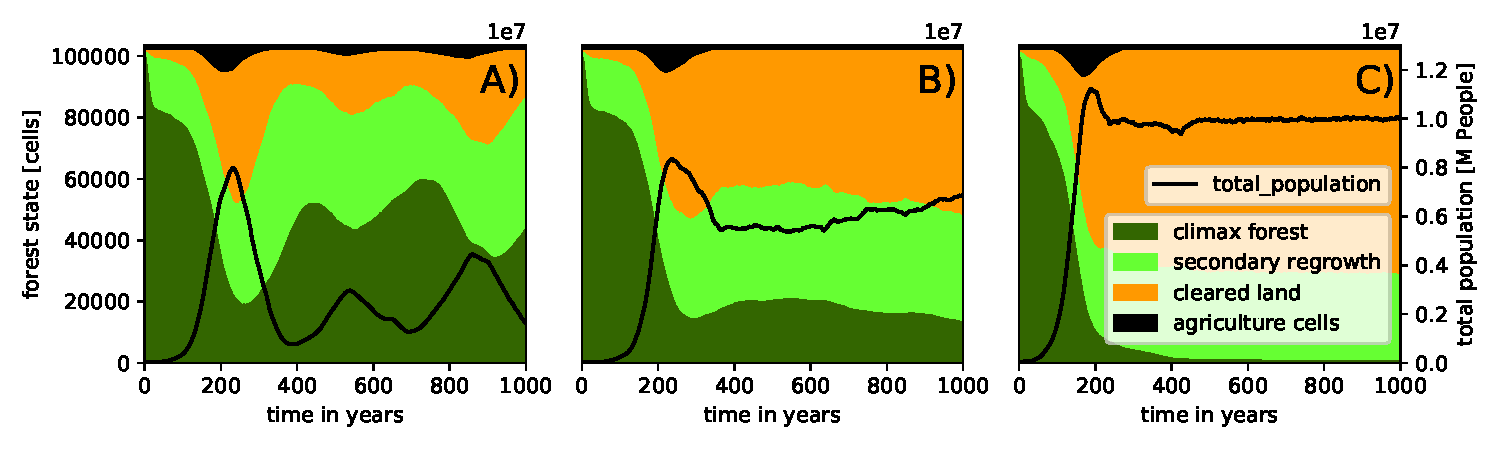
\includegraphics[width=\textwidth]{figures/trajectory.pdf}
\caption{\textbf{Example trajectories of simulation runs} with different possible income from trade relations $r_{trade}$. Possible income from trade relations increases from A: $r_{trade}=6000$, B: $r_{trade}=7000$ to C: $r_{trade}=8000$. The colored stack plot shows the fraction of land in different states on the left axis. The black line shows the total population on the right axis.}
\label{fig:trajectory}
\end{figure}

\subsection{Bifurcation Analysis}
%\textit{Is the overshoot and collapse reported with the original model inherent or rather a result of parameter choices and selection of the time window?}
% Motivate the variation of $r_{trade}$ and $r_{es}$.

Income per capita is the main driver of population growth in the Mayasim model. Income is calculated as a linear combination of three different sources of income: agriculture, ecosystem services and trade. The parametrization of income from agriculture can be sensibly done as e.g. in \cite{ertsen2018}. However, the parameters for income from trade $r_{trade}$ and ecosystem services $r_{es}$ are more difficult to calibrate. Therefore, I analyze their influence in more detail in the following.

% Discuss the trajectories for different values of r_trade

Results from model runs with different choices of $r_{trade}$ are shown in figure \ref{fig:trajectory}. For different choices of the possible income from trade, the model exhibits fundamentally different dynamics:
\begin{itemize}
  \item In fig. \ref{fig:trajectory} A the total population and the aggregate number of climax fores cells exhibit a predator prey like dynamic that can be explained as follows: Climax forest results in soil regeneration as well as a high level of ecosystem services which drives per capita income and thereby population growth. Growing population on the other hand leads to disruption of the fores ecosystem resulting in its degeneration as well as extensive agriculture, that benefits from regenerated soils but also drives clearing of forest and soil degeneration.
  \item In fig. \ref{fig:trajectory} B higher possible income from trade leads to the onset of the decoupling of population dynamics from the state of the surrounding ecosystem. 
  \item In fig. \ref{fig:trajectory} C the society, once in its complex state characterized by strong trading relations, is no longer dependent on the state of the surrounding ecosystem.
  \item A closer look at the results in fig. \ref{fig:trajectory} A also shows that they are not just a result of a simple predator prey dynamic but rather represent a pattern of of regionally increasing complexity, collapse and restructuring not unlike what the archeological record from the area suggests.
\end{itemize}
These results also suggest, that the initial overshoot and collapse dynamics presented in \cite{Heckbert2013} may have been only part of the picture. The results suggest that the pronounced overshoot and collapse is at least partially caused by the initial conditions that combine a perfectly intact ecosystem with a small initial population that, given the modeling choices is implicitly assumed to have full knowledge of agricultural techniques, trade and ecosystem usage. They show, that after the initial overshoot and collapse a more balanced feedback between human settlements and the surrounding ecosystem is possible as displayed in \ref{fig:trajectory} A.

\begin{figure}[!t]
\centering
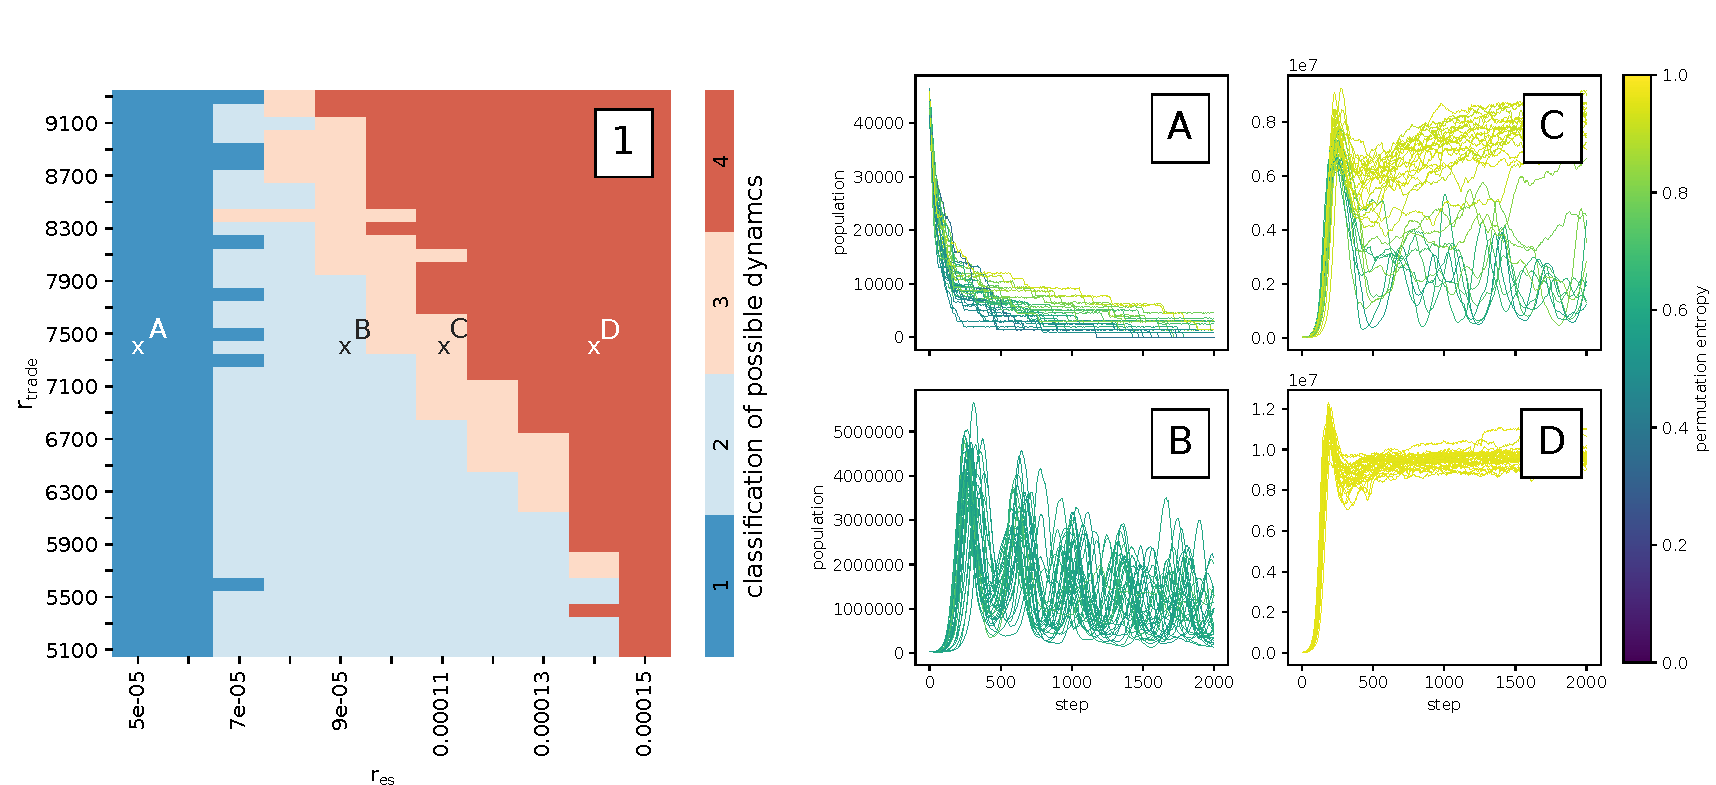
\includegraphics[width=\textwidth]{figures/classified_dynamics.pdf}
\caption{\textbf{Classification of model dynamics for different values of income from trade relations and ecosystem services.} Results are calculated from an ensemble of 30 runs for each combination of parameter values. For each of these 30 runs, I calculate the permutation entropy of the trajectory for $t>500$ i.e. after the initial overshoot and collapse. I show sets of trajectories for different parameter values in panels A, B, C and D. The color of the trajectories indicates their permutation entropy. The specific parameter values are marked in panel 1. From the distribution of the permutation entropy of these ensembles of trajectories, I classify the dynamic regime of the model given in panel 1. Regime 1 indicates the monotonous decline in population as in panel A, regime 2 indicates oscillatory behavior of the population as in panel B, regime 4 indicates a stable high population state as in panel D and regime 3 indicates the coexistence of the two aforementioned dynamics as in panel C.}
\label{fig:permutation_entropy}
\end{figure}

% Discussion of different possible dynamic regimes / bifurcation analysis

To systematically expand on this finding, I generated model trajectories for a wide range of values
for the possible income from trade relations and the possible income from ecosystem services in the model and classified the resulting trajectories with regards to their dynamical properties. A suitable measure for this task is permutation entropy as introduced by \cite{Bandt2002}. This measure classifies trajectories by interpreting them as a series of ordinal patterns of a predefined length and then calculating the entropy of the distribution of said patterns. This entropy is normalized between zero and one. To give some points of reference: For a constant trajectory, this results in a permutation entropy of zero. For a sine wave, this results in a value of one half and for uniformly distributed noise, this results in a value of one.

The classification of the dynamical properties of the model for different parameter values is given in fig. \ref{fig:permutation_entropy} 1. It shows that the model exhibits a bifurcation like behavior where depending on the parameter values different qualitative behaviors are possible. First, a slow decline in population that eventually leads to extinction as displayed in fig. \ref{fig:permutation_entropy} A, second, an oscillatory with a predator prey like dynamic between the Maya population and the forest ecosystem fig. \ref{fig:permutation_entropy} and also fig. \ref{fig:trajectory} A, third, a stable state with high population that is primarily supported by income that is generated from trade as in fig. \ref{fig:permutation_entropy} D and fig. \ref{fig:trajectory} C and fourth, a region where oscillatory behavior and stable high population states can coexist as in fig. \ref{fig:permutation_entropy} C.

% Discussion of stable high population regime that is primarily supported by trade income

Particularly the stable high population state deserves a closer look. As fig. \ref{fig:trajectory} C shows, this state is characterized by low agricultural activity and a degraded ecosystem such that income from trade is the primary source of income. Even though the particulars of trade theory are controversial among economists, there is consensus in that increase in welfare through trade originates in either better division of labor or exchange of locally different input factor endowments. This means, that income from trade without other sources of economic productivity is not a realistic scenario. This sheds light on the limits of the trade model that is used in the MayaSim Model where income from trade is generated through the establishment and maintenance of a trade network amongst sufficiently large settlements i.e. through societal complexity alone. This is a plausible approximation as long as there are substantial sources of income other then trade but becomes unrealistic as soon as trade becomes the primary source of income and even more, once income from trade stabilizes the high population levels that are necessary to sustain the trade relations that generated said trade income to begin with.

Therefore, I conclude that the stable high population attractor is a pathological consequence of the approximate implementation of trade in the model and can be discarded for considerations about the archeological realities of the ancient Maya.
Consequently, for the following analysis of system resilience with respect to drought events, I use parameters that lead to oscillatory behavior where income from trade relations can be considered realistic.

% Discussion of results from drought events.

\begin{figure}[ht]
\centering
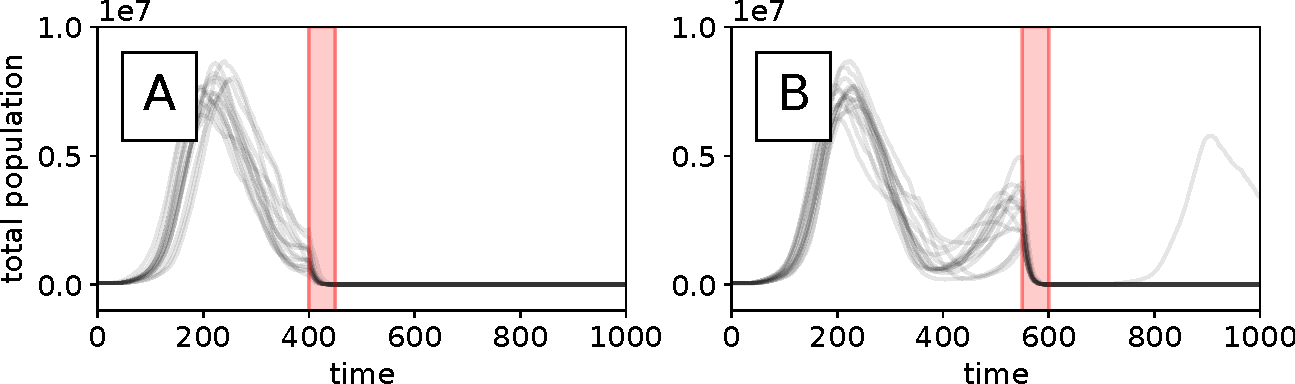
\includegraphics[width=\textwidth]{figures/population_with_drought.pdf}\vspace{.3 cm}
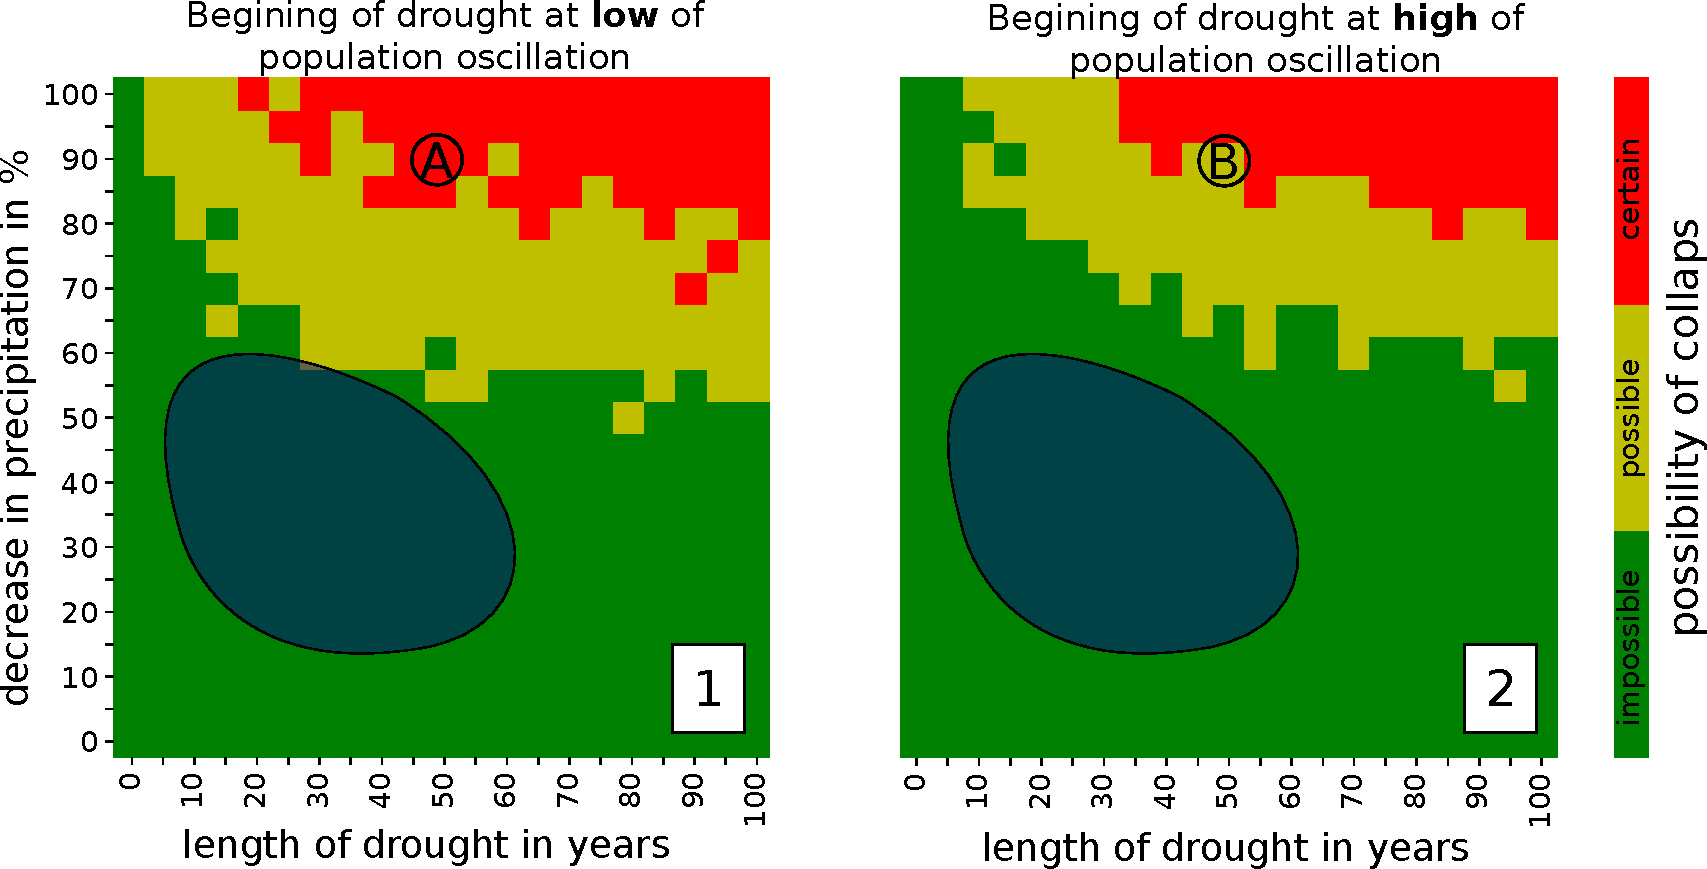
\includegraphics[width=\textwidth]{figures/possibility_of_collapse.pdf}
\caption{\textbf{Measurement of Transformation-Resilience with respect to drought events of different length, severity and timing compared to estimates from paleo-climatic data.} Results are calculated from an ensemble of 15 simulation runs for each combination of drought length and severity. Panels 1 and 2 differ with respect to the timing of drought events. In panel 1 the beginning of the reduction of precipitation starts approximately at the bottom of the oscillations of total population whereas in panel 2 it starts at its top. To illustrate this, panels A and B show individual trajectories of the total Maya population for drought events of the same length and severity but with different timing. Parameter values for length and severity of drought events in panels A and B are also marked in panels 1 and 2 respectively.
I classify resilience in terms of the possibility of collapse i.e. extinction of the human population for drought events of different length, severity and timing.
Technically, this means that I disregard the systems micro state and only estimate the probability for for a drought event to force the social ecological system out of the basin of attraction of its habitable attractor and then classify the parameter space of length and severity of drought events in regions where this probability is either zero, one or in between. These regions are marked in green, yellow and red respectively in panels A and B. The region of parameter values for length and severity of drought events that can be motivated by evidence from paleo-climatic records is marked in blue in panels 1 and 2.}
\label{fig:stability_analysis}
\end{figure}

\subsection{Drought Resilience}
\textit{Can a drought event be responsible for the terminal decline of the Maya civilization on the Yucatan peninsula, given the assumptions of the model?}

As discussed in the methods section, the ability of the system to recover after a large scale disturbance to a state that is macroscopically equivalent to that before the disturbance -- regardless of their microscopic configuration -- can be seen as a measure of resilience with respect to said disturbance.

To better understand the possibility of a large drought event leading to a lasting change in the Mayan population on the Yucatan peninsula, I analyse the models resilience to such drought events of different length, severity and timing. The results in fig. \ref{fig:stability_analysis}, panel A and B show the trajectories of total population for different model runs with equal model parameters but different timing of drought events. In panel A a drought event with length of 50 time steps and precipitation reduction of 90\% starts as the oscillation of population levels is a low. This leads to the complete disappearance of the Maya population in all simulated cases. A drought event of the same magnitude but beginning at the peak of the oscillation as in panel B also results in a severe reduction in population over the time of the drought event. However, if a small population survives, it is able to recover and to reach population levels comparable to those before the drought event.

To analyze the impact of drought events systematically, I show results for drought events with timing like in panels A and B but for different length and severity in panels 1 and 2. To abstract from the presentation in terms of trajectories, I classify the results of an ensemble of model runs for each set of parameter values in the following way: If in all model runs, the Maya population vanishes, I say that collapse is certain and mark the parameter combination red. If this happens only in some of the model runs, I say that collapse is possible and mark the parameter combination in yellow and if the Maya population vanishes in none of the simulation runs, I say that collapse is impossible and mark the parameter combination in green.

These results show, that the timing of drought events does have the effect on the measured resilience that can also be expected. A drought of the same length and severity can have a more dire effect if it hits at the moment when population levels are already low.

This abstract representation of the impact of drought events enables us to draw a comparison with the paleo-climatic evidence available:
\cite{Stahle2011} find evidence for drought of 25y duration but make no estimate for precipitation reduction.
\cite{Evans2018} estimate a reduction in annual precipitation of 41\%-52\% with up to 70\% during peak drought but no make specification as to the length of drought events.
\cite{Medina-Elizalde2010} find evidence for six droughts between C.E. 800 and 909 with a maximum reduction in annual precipition of ~52\% and a maximum length of 18 years.
\cite{Medina-Elizalde2012} estimate a reduction in annual precipitation of 25\% to 40\% over more than 14 years.
\cite{Kennett2012} mention a -40\% reduction in annual precipitation between 820 and 870 C.E. as well as a 100 year drought starting in 1020 C.E.


Overall the different estimates for historic drought events reach from a reduction of annual precipitation of 25\% to 52\% over an extended period of 25 up to 50 years. I mark this region in blue in fig. \ref{fig:stability_analysis} panel 1 and 2 for comparison.

This comparison shows, that even with unfortunate timing of drought events, the values for length and severity of drought events that can be motivated from paleo-climatic records has quasi zero intersection with the parameter values that possibly lead to extinction of the Maya population in our model.

I conclude, that given the economic and behavioral assumption about the Maya civilization that are the basis of the MayaSim model, drought events alone are a very unlikely cause for a long lasting severe impact on the Maya civilization on the Yucatan peninsula.

\section{Discussion and Conclusion}

% Short recap of paper
This paper reimplements and improves upon an established/existing agent-based geosimulation model for the ancient Maya civilization on the Yucatan peninsula.
I analyze the model with respect to sensitivity to key parameters and find that is capable of a richer dynamic variety than presented in the original studies.
I also analyze the resilience of the model dynamics with respect to drought events compare the results with data from paleoclimatic records.

% comparison of our model dynamics to Heckberths original results
The origininal study \citep{Heckbert2013} and reference implementation \citep{Heckbert2013model} of the MayaSim model presents an overshoot and collapse pattern of the ancient Maya civilisation and attributes the cause of the collapse to changing climatic conditions, specifically decreasing annual precipitation in the region. After a close examination of the reference implementation and comparing its results with the results of our improved implementation with come to a different conclusion. I rather propose to attribute the pronounced overshoot and collapse pattern of the original model to two particular modelling choices in combination with the models initial conditions. Namely the fact that in the original implementation settlements were deleted if and only if they abandon their last agriculture cell in combination with the choice to model income from agriculture and ecosystem services as the mean rather than the sum of income from cells that are used for ecosystem services and agriculture respectively. This means that even a large settlement can survive on the income from one cell of agriculture only to suddenly vanish, once this last patch of agriculture becomes uneconomic. On an aggregated level this means that the feedback from the deteriorating ecosystem due to deforestation and soil erosion impacts the settlement infrastructure delayed but then suddenly all the more forceful. In combination with the initial condition of a small population in a fully intact ecosystem that can quickly expand without feeling the effects of its unsustainable growth this strongly supports the observed pattern.

In our updated model, I chose to model these two processes differently and as I believe more credibly. I model income from agriculture and ecosystem services as the sum of income that is generated from individual cells that are under a settlements influence and I model the abandonment of settlements such that they are deleted once their population drops under a minimum threshold that is necessary for subsistence.

This means that the effect of the deterioration of the surrounding ecosystem impacts the affected settlements directly and without delay. Consequently, the initial overshoot is less pronounced in our adaptation of the model. However, I also find that following the initial overshoot this adaptation produces a pattern of development, climax, deterioration and spatial reorganization of regional centers in close interdependence with the surrounding ecosystem that much resembles the archeologic record. I find that this oscillating dynamic strongly depends on the parameterization of the model and that for variation of key parameters the model undergoes two transitions. The first transition leads from a state where the initial population continuously deteriorates to eventually vanish to the previously described state of cyclical rise and fall of regional centers. The second transition leads from this state of cyclical dynamics to another state of stable, self sustaining high population in a deteriorated ecosystem. Of these, only parametrizations that lead to cyclical behavior of the model can be considered realistic.

% discussion of results from analysis of model resilience w.r.t. drought events
Subsequently, I test the resilience of the updated model with a realistic parameter setting with respect to drought events of different severity, duration and timing. In this study I find that even for drought events that even drought events that reduce the mean annual precipitation to half for a duration of 50 hears do not lead to the extinction of the Maya population in the model. This holds true even if the drought event hits the population in a state where it is deteriorized to begin with due to its inherent dynamics. Comparing these results with the length and severity of drought events that can be motivated from historical records, I find that none of them would be sufficient to eventually break up the Maya civilization in the model.
From this I conclude that given the assumption that the model is grounded on, climate variability as single cause of the deterioration of the ancient Maya civilization can be ruled out. Rather this supports the argument that in addition to climate variability other factors had to play a role in the fundamental transformation of the Maya society during the Terminal Classic Period \citep{Masson2012}. Others have also already argued that in only internal societal changes could have caused this transformation under the conditions of increased aridity and overly stressed ecosystems \citep{Turner2012a}.

% discuss how models could better picture societal change on an individual level
One way to address this this problem from a modeling perspective would be to separate judgement from actions in the modeling of individual (human) agents. Possible actions are usually confined to a finite set that is limited by the conditions of the agents environments but judgements can evolve more freely as a way to  allow agents to change. Technically, this can be implemented e.g., with techniques from reinforcement learning \citep{Bu2008} or by implementing different heuristic decision models. Such heuristic decision models allow for an adaptive mental model of individual agents in terms of simple algorithmic rules that they use to integrate the information from their environment to select one of different possible actions.
This would allow for agents to adapt to changing circumstances in their modeling environment. While modeling paradigm does not change the fundamental fact that agents in a model cannot have anything resembling free will, it would nevertheless allow for models to depict changes in societal structure that are grounded in individually changing perceptions of reality.


        \chapter{General Introduction}
This general introduction has to cover the following topics:
\section{Agent-Based Modeling}
Definitely.
\section{`World-Earth' Modeling}
Also has to be in there. But not sure w.r.t. to the framing and wording.
With reference to the Copan Core framework paper
\section{Heuristic Decision Making}
Definitely. With reference to the section in Finns review paper
\section{Adaptive Networks and Aggregation Methods?}
Not so sure. But I can still decide on that later.

%        \chapter{Methods}
Not completely clear, whether I actually need a methods section.

        \chapter{Heuristic Decision Making in a Economic Model of Fossil Resource Usage}
\label{chapter:heuristics}
This chapter is based on unpublished work. However, a simplified version of the economic model is part of \citep[P5]{Kolb2019b}.
\section{Introduction}

In the IPCCs current business as usual scenarios, the CO$_{2}$ emissions budget that limits global warming to below 1.5$^{\circ}$C with a likelihood of 0.5 will be exceeded by approximately 2030. This means that in order to limit global warming below 1.5$^{\circ}$C, the global economy needs a rapid shift away from fossil fuel based technologies. Currently, the two main measures that are expected to incentivize the necessary changes are taxation and cap and trade schemes for CO$_{2}$ emissions. I suspect that these measures are favoured by many because they are expected to be efficient. This is most likely because their effects are thought to be adequately understood as they can be estimated well with the current integrated assessment models that are used to generate the economic projections for the IPCCs reports. However, there are some issues with these policy measures. First, the expected effects of these policy measures are estimated in an idealized model world whereas their real effects come from their real implementation that might include a number of exceptions, loopholes and unintended consequences. And second, with few exceptions, the political process to implement these measures is sluggish and the outcomes are all but certain.

Therefore, I argue that in addition to top down policy measures, bottom up initiatives are essential to successfully mitigate global warming. 
There are a number of such bottom up initiatives such as Fridays for Future or Extinction Rebellion that are currently gaining more and more traction. These initiatives use means of collective and direct action make their claims and to influence public discourse. The analysis of similar movements shows that their dynamics are essentially driven by opinion formation and individual decision processes amongst heterogeneous individuals \citep{Graeber2009, Engler2016}. Consequently, as discussed in section \ref{sec:intro_complex_systems}, the models that are currently used for climate change mitigation scenarios are unable to picture them due to their reliance on a representative agent approach.

With this motivation I develop a conceptual economic model of fossil resource use and technological change that is able to explicitly depict individual decision making of heterogeneous agents, as well as social learning and opinion formation in order to better understand the possible effects of social movements in mitigating global warming.

This model combines individual decision making via a simple fast and frugal decision heuristic and interactions between individuals via a social learning process with feedbacks on an aggregated supply and demand level in a two sector investment economy.

In the reminder of this chapter, I will outline and explain this model in section \ref{sec:heuristics_model}, simplify it analytically as far as possible and explore some of its limiting cases in sections \ref{sec:algebraic_constraints} and \ref{sec:limiting_cases} and fit its parameters to past economic data in section \ref{sec:parameter_values}. Subsequently, I analyze the models default dynamics in section \ref{sec:default_scenario} and showcase the possibility to analyze a stylized social movement with this model in section \ref{sec:campaign} before concluding.

\section{Model Development}  
\label{sec:heuristics_model}
Previous studies by \cite{Ans2013} suggest that feedback through supply-demand price mechanisms will have only limited impact on fossil fuel companies. This is due to the fact that only approximately 15 \% of investors invest subject to socially responsible guidelines \citep{SIF2014Report} and that divested holdings are, especially in liquid markets, very likely to quickly find their way to less responsible investors. \\
Also, as long as the physical capital relying on fossil fuels already exists, economic reasoning follows that it will be used as long as variable costs are covered.
Therefore, a general economic shift from dirty to clean technology needs changes in investment in physical capital or a political imperative mandated by a (qualified) majority. Therefore, I consider a model focussing on savings and investment decisions appropriate to investigate the possible dynamics of an economic transition towards fossil resource independent technologies.\\
In the following I propose a preliminary scheme of such a model.
\begin{figure}[t]
	\centering
	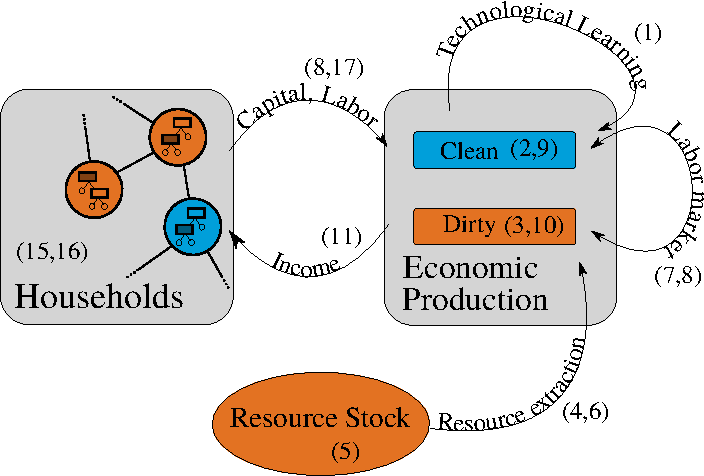
\includegraphics[width =.8 \textwidth]{figures/model_scheme_1.pdf}
        \caption[Schematic sketch of a two sector investment model with heterogeneous households that are bounded rational decision makers]{Schematic sketch of the model consisting of two production sectors (a \emph{clean} and a \emph{dirty} one) and heterogeneous households that are heuristic decision makers that interact on a complex adaptive acquaintance network. Households supply labor and capital to the production sectors. The production sectors each have their separate capital market but are linked via a shared labor market. The \emph{dirt} sector depends on the input of an exhaustible fossil resource, the \emph{clean} sector depends on a developing technology that is endogenously modelled via learning by doing. Boxes and bubbles signify modelled entities, arrows signify interactions. Numbers ($x$) next to entities and interactions give the decimal place of equations in the model description section \ref{sec:model_description} that describe the respective processes.}
	\label{fig:model}
\end{figure}

\subsection{Economic Production}
\label{sec:model_description}

As illustrated in \cref{fig:model}, the model consists of two sectors for production and a set of heterogeneous households that interact via an adaptive complex social network. The production sectors employ different technology. I call them the \textit{clean} and the \textit{dirty} sector for illustrative clarity. The heterogeneous households in the model provide capital $K$ and labor $L$ to both sectors.
In addition, the production technology in the dirty sector depends on the input of an exhaustible (fossil) energy-resource $R$ that is used up in the process. I assume that the technology in the dirty sector is fully developed and adequately described in terms of the total factor productivity. 
Price elasticities\footnote{The price elasticity of demand ($PED$) for a good describes the change in demand $Q$ for that good when the price of that good $P$ (and nothing else) changes. Formally, it is defined as $PED = \partial Q / \partial P \times P/Q$. Informally this means that if the price elasticity of a good is low, it will be bought in similar quantities regardless of rising prices.} of demand for fossil fuel are evidently low in real economies \citep{IMF2011, Hosslinger2017, Labandeira2017}, even with the choice between alternative technologies factored in. I approximate this by setting the marginal rate of substitution\footnote{The marginal rate of substitution $MRS_{12}$ of two goods $G_1$ and $G_2$ describes the extent to which good $G_1$ can be replaced by good $G_2$ in a given economic process. More precisely, in this case it would be called the marginal rate of \emph{technical} substitution as it refers to the substitution of two goods in a production process (as opposed to the substitution of goods in consumption). Technically, it is defined as 
\begin{equation}
  MRS_{12} = \frac{\partial Y(G_1,G_2)}{\partial G_1} / \frac{\partial Y(G_1, G_2)}{\partial G_2} \nonumber
\end{equation}
where $Y(G_1, G_2)$ is the economic production function that links the input of goods $G_1$ and $G_2$ to economic output $Y$. In effect, this means that when the marginal rate of technical substitution between two goods is zero, they cannot be replaced by one another in a production e.g., when one of the goods is missing, production halts regardless of the quantities of the other good that are available.} between the fossil resource and the pair of capital and labor to zero in the dirty sector. This is also in line with contemporary critique of the neoclassical growth models \citep{Daly1997,georgescu1975energy,georgescu1979comments, Ayres2007, Ayres2013} that highlights the generally assumed substitutability of natural resources in production as being physically implausible and lacking empirical evidence.

I acknowledge the common argument for substitutability between capital, labor and energy resources due to a shift in the output of economic production from manufacturing to services and would argue that this model pictures this in a shift of economic production from the dirty sector to the clean one which is described in the following.

The clean sector represents a circular economy in which the output of final goods depends on the machinery, knowledge and effort used in its production and is not limited by entropy laws or resource scarcity on the timescale under consideration. The technology $C$ used in the clean sector is assumed to be still in development and is therefore explicitly modeled.
Following \cite{argote1990learning}, I model technological process as learning by doing according to Wright's law \citep{wright1936factors, Nagy2013} with a one-factor learning curve. I assume that $C$ is proportional to cumulative production but also depreciates with a constant rate $\chi$. 
\begin{equation}
	\dot{C} = Y_c - \chi C.
	\label{eq:learning_by_doing}
\end{equation}
Depreciation can be regarded as a human capital effect that leads to knowledge depreciation over time \citep{Kahouli-Brahmi2008}. This is also in line with the empirically observed decrease in learning rates for maturing technologies \citep{argote1990learning}
In the clean sector, capital $K$, labor $L$ and technology/knowledge $C$ are assumed to be mutual substitutes. To satisfy these requirements, I use the following production functions:
\begin{align}
	Y_c &= b_c C^{\gamma} L_c^{\alpha_c}K_c^{\beta_c}, \label{eq:clean_production} \\
	Y_d &= \mathrm{ min}\left( b_d L_d^{\alpha_d}K_d^{\beta_d}, e R \right), \label{eq:dirty_production}
\end{align}
Subscripts $c$ and $d$ denote the clean and dirty sector respectively, $Y_c$ and $Y_d$ are their economic outputs and $L_c$ and $L_d$ are labor shares in each sector. $\alpha$ and $\beta$ are elasticities of the respective input factors and $b_c$ and $b_d$ are the total factor productivity and $K_c$ and $K_d$ are the capital stocks for the respective sector.
% Measuring unit production cost in the number of working hours as in the original study by Wright \cite{wright1936factors}, $\gamma$ is equivalent the elasticity of learning by doing in the clean sector as outlined in \cite{Kahouli-Brahmi2008}.
% This is probably too much info and confusing for a physics audience.

The structure of eq. \ref{eq:dirty_production} implies that if $b_d L_d^{\alpha_d}K_d^{\beta_d} \ne e R$, either capital and labor or fossil resource would be available in excess but unused and idle, which would be inefficient. I assume efficient an usage of resources in the dirty sector, such that
\begin{equation}
    b_d L_d^{\alpha_d}K_d^{\beta_d} = e R
    \label{eq:efficient_dirty_resources}
\end{equation}
where $1/e$ is the resource intensity of the sector. The usage of the fossil resource $R$ depletes a geological resource stock $G$ with the initial stock $G(t=0) = G_0$:
\begin{equation}
    \dot{G} = -R. 
    \label{eq:resource_depletion}
\end{equation} 
In line with the assumptions common in the literature \citep{Dasgupta1974, Perman2003}, the total cost $c_R$ for the usage of the fossil resource depends on the resource use $R$ and the remaining fossil resource stock $G$ such that total resource costs increase with resource use ($\partial c_R / \partial R >0$) and also with continued resource depletion ($\partial c_R / \partial G < 0$). I chose the specific form to be
\begin{equation}
	c_R = b_R R^{\rho}\left( \frac{G_0}{G} \right)^{\mu}; \quad \rho \geq 1, \quad \mu > 0,
	\label{eq:resource_cost}
\end{equation}
such that at some point $\partial Y_d / \partial R < \partial c_R / \partial R$ to take into account that some part of the resource is not economic, e.g. its marginal cost exceeds its marginal productivity.
Perfect labor mobility and competition for labor between the two sectors lead to an equilibrium wage $w$ that equals the marginal return for labor:
\begin{equation}
	w = \frac{\partial Y_c}{\partial L_c} = \frac{\partial Y_d}{\partial L_d} - \frac{\partial c_R}{\partial L_d}
	\label{eq:equilibrium_wage}
\end{equation}
with the sum of the labor shares equal to the total amount of labor available:
\begin{equation}
	L_c + L_d = L.
	\label{eq:population}
\end{equation}
I assume physical capital to be specific to the technology employed such that it can only be used in the sector that it has been invested in originally, resulting in separate capital markets for the two sectors. I assume these capital markets to be fully competitive resulting in capital rents equal to marginal productivity:
\begin{align}
	r_c &= \frac{\partial Y_c}{\partial K_c} \label{eq:clean_capital_rent}\\
	r_d &= \frac{\partial Y_d}{\partial K_d} - \frac{\partial c_R}{\partial K_d} \label{eq:dirty_capital_rent}
\end{align}

\subsection{Investment Decision Making}
\label{sec:investment_decision_making}
I model households as bounded rational decision makers \citep{simon1972theories, simon1982models, gigerenzer2002bounded}.
That is, households take their investment decisions, i.e. whether to invest their savings in the clean or the dirty sector, not by forming rational expectations \citep{Evans2006, Kirman2014} but by A) using \emph{heuristic decision strategies} to make robust decisions with sparse information and with limited computational work and B) engaging in \emph{social learning} \citep{Bandura1971} to obtain successful decision strategies \citep{Traulsen2010} with reasonable effort.

% Why use Fast and Frugal heuristics for decision making?
Regarding individual decision making, there is ample evidence that real investors rather use a diverse set of heuristic strategies to make investment decisions. \cite{Gigerenzer2018} and other researchers in the field strongly suggest to consider these so called \emph{Fast and Frugal heuristic} decision models as a complementary alternative to established probabilistic and optimizing decision models. 
In general, Fast and Frugal Heuristics are described in terms of three building blocks; one for information search, one for stopping information search and one for evaluating the available information and drawing a conclusion from it.
I use a decision heuristic called \emph{Take The Best} that is observed to be frequently used in situations where individuals need to decide between one of two options that are comparable in different aspects \citep{gigerenzer1999simple, Newell2003a}. 
Take the Best has the following building blocks: 1) Search through cues in a predefined order, 2) stop as soon as one cue discriminates between the two options, 3) chose the option with the preferable value on the discriminating cue. \\
This requires a so called \textit{cue order} e.g.\ a hierarchy of validity for the pieces of information that are considered relevant for the decision. \\

% How these heuristics can be interpreted in this context.
Research on perception and decision making in psychology where the concept of Fast and Frugal heuristics was developed usually considers inferential decisions (since they have true and false outcomes and can therefore be benchmarked and evaluated statistically).\\
Nevertheless, Heuristic decision making is a reasonable tool for preferential decisions as well. Although in this context the interpretation of cue orders would be different - namely, they would rather be considered as norms or underlying preferences that apply to the context of the decision. \\
The case of savings decisions that is considered in this model poses an intermediate case between preferential and inferential decisions for a number of reasons. First, there is no immediate feedback on savings decisions, since the return on investment depends on the future development of the economic system which again depends on the savings decisions of all other households and second, I assume that households do not only consider financial but also moral grounds for their savings decisions.
Additionally, I argue that imitation of peers is not only an efficient learning strategy in many situations but also a value in its own - especially if the question is to some extend ethical. 

% Heuristics can be learned from others. This is why we model social learning.
Nevertheless, some strategies are suspected to have more profitable long term results then others as the performance of this decision heuristic depends on the order of the sequence of cues \citep{Gigerenzer2011}. Empirical evidence shows that if participants in an experiment are allowed to share information about their cue orders and respective performance, they do so and thereby greatly increase the speed of learning of cue orders that fit their decision environment compared to individual trial and error reinforcement learning \citep{garcia2009does}. Therefore, I use social learning among households to determine the particular cue order that determines their investment decision making.

% As the outcomes of social learning depend on network topology, we model topology endogenously.
As the outcomes of social learning crucially depend on the structural properties of the complex network of social ties amongst the households \citep{Barkoczi2016}, I model the adaptive formation of this social network endogenously.
A well established principle for the emergence of structured ties in social networks is homophily, i.e. the tendency that similar individuals are linked \citep{McPherson2007, Centola2007, Centola2011}. Especially the concept of value homophily \citep{McPherson2007} is in line with the interpretation of cue orders above not only as a means to the end of making profitable investment decisions but also as an expression of identity and beliefs with regards to clean technology.
The following model specification uses social learning in combination with endogenous network adaptation based on homophily to model the changes in heuristic decision strategies that households use to make investment decisions.

% How I do this technically (Individual Household earnings and investment)
I model $N$ heterogeneous households denoted with the index $i$ as owners of one unit of labor $L^{(i)} = L/N$ and capital $K_c^{(i)}$ and $K_d^{(i)}$ in the clean and dirty economic sector respectively.
Households generate an income $I^{(i)}$ from their labor and capital income which they use for consumption $F^{(i)}$ and savings $S^{(i)}$:
\begin{align}
	I^{(i)} &= w L^{(i)} + r_c K_c^{(i)} + r_d K_d^{(i)}, \label{eq:household_income} \\
	F^{(i)} &= (1-s) I^{(i)}, \label{eq:consumption} \\
	S^{(i)} &= s I^{(i)}. \label{eq:savings}
\end{align}
A binary decision parameter $o_i \in [c,d]$ denotes the sector in which the households decide to invest and $s$ denotes the savings rate at which households reinvest their income. As motivated above, I model decision making that is driven by three processes: Heuristic decision making via the Take The Best heuristic, social learning via the imitation of successful cue orders and homophily towards individuals exhibiting the same beliefs as represented by its cue order. \par

% How I do this technically (Heuristic and cue order here)
Concerning the information that households use to make their investment decisions, they are assumed to be unable to form rational expectations about the future, e.g.\ they make decisions based solely upon information about the past and present. Possible sources of information are economic indicators such as capital rents in both sectors $r_c$ and $r_d$ and their trends $\dot{r}_c$ and $\dot{r}_d$ as well as observable behavior of other households that they are connected to via the social network and subjective beliefs of superiority of one over the other sector that are not explained by other factors.\\
Each household is characterized by a cue order $O$ containing some or all of the above cues in a specific order. At each time, it uses the Take the Best Heuristic with this cue order to evaluate the information that is available and make an investment decision accordingly.
\par

% How I do this technically (social learning of cue orders)
I describe households as the nodes in a graph of acquaintance relations. Households get active at a constant rate $1/\tau$. When a household $i$ becomes active, it interacts with one of its acquaintances $j$ chosen at random. If they follow the same strategy, i.e. they share the same cue order $O$, nothing happens. If they follow a different strategy, i.e. they differ in their cue order, one of two actions can happen:
\begin{itemize}
	\item Homophilic network adaptation: with probability $\varphi$, the households end their relation and household $i$ connects to another household $k$ that has the same cue order. 
	\item Imitation: with probability $1-\varphi$, household $i$ engages in social learning i.e. it imitates the cue order of household $j$ with a probability $p_{ji}$ that increases with their difference in income.
\end{itemize}
I follow previous results on human strategy updating in repeated interactions \citep{Traulsen2010}, when I assume the imitation probability as a monotonously increasing function of the relative difference in consumption between both households:
\begin{equation}
	p_{ji} =  \left(1 + \exp \left(- \frac{a(F^{(i)} - F^{(j)})}{F^{(i)} + F^{(j)}} \right) \right)^{-1}.
    \label{eq:imitation_probability}
\end{equation}
As opposed to the absolute difference in the original study \citep{Traulsen2010}, the probability in this model depends on relative differences. This dependence on relative differences in per household quantities is crucial for approximation methods as I will discuss later at the end of \ref{sec:large_system_limit}.
I set $a = 8$ to conform to their empirical evidence.
I model strategy exploration as a fraction $\varepsilon$ of events that are random, e.g. rewiring to a random other household or randomly choosing one of the possible cue orders with equal probability.

% Yes, we know, this is only one of the many possible ways to implement such a model.
I acknowledge the fact that different model specifications are possible and interesting.
For instance, I only consider fixed savings rates and the decision between two capital assets and return to the investigation of households setting their savings rates individually in \cref{chapter:savings}.
Also, this framework might as well be used to test other strategies for decision making such as tallying or pure social learning similar to the approach taken by \cite{Barkoczi2013, Barkoczi2016}.

% Capital accumulation of individual households given the model assumptions above.
Given the savings decisions of the individual households, and assuming equal capital depreciation rates $\kappa$ in both sectors, the time development of their capital holdings is given by
\begin{align}
  \dot{K}_c^{(i)} =& s\delta_{o_ic} \left( r_c K_c^{(i)} + r_d K_d^{(i)} + w L_i \right) - \kappa K_c^{(i)}, \label{eq:clean_investment}\\
  \dot{K}_d^{(i)} =& s\delta_{o_id} \left( r_c K_c^{(i)} + r_d K_d^{(i)} + w L_i \right) - \kappa K_d^{(i)}, \label{eq:dirty_investment}
\end{align}

where $\delta_{ij}$ is the Kronecker Delta. The total capital stocks in the two sectors are made up of the sum of the individual capital stocks as
\begin{equation}
K_j = \sum_i^N K_j^{(i)} = N k_j,
\end{equation}
where $k_j$ is the average per household capital stock of a given capital type.


% This is the model. Now lets see what it does.
With the model specifications from above, the parametrization in Tab.~\ref{tab:Parameter_list} and appropriate initial conditions for the dynamic variables, the model can be numerically simulated.
For this, I implemented the dynamics in the multi-purpose programming language python. The implementation of the agent based model, as well as the numerical analysis using the approximation methods described in the following are available on github in \cite{kolb2018}.
In the following, I discuss the technical details ans specification of this implementation.

\begin{table}[t]
	\centering
	\begin{tabular}{r|l}
		Variable & Description \\\hline
		$O_i(t)$ & opinion/cue order of household $i$ \\
		$K^{(i)}_c(t)$ & clean capital of household $i$ \\
		$K^{(i)}_d(t)$ & dirty capital of household $i$ \\
		$G(t)$ & fossil resource stock \\
                $C(t)$ & knowledge stock in the clean sector \\\hline
		$o_i(t) \in [c,d]$ & investment decision of household $i$ \\
		$Y_j(t)$ & output of sector, $j$ \\
		$L_j(t)$ & total labor employed in sector $j$, \\
		$K_j(t)$ & total capital employed in sector $j$, \\
		$w(t)$   & wage rate, \\
		$r_j(t)$ & capital return rate in sector $j$, \\
		$c_R(t)$ & fossil resource extraction cost, \\
		$R(t)$ & rate of resource uptake of dirty sector. \\
	\end{tabular}
        \caption[Model variables with description]{Variables of the model and their description - entries in the first section are free variables (minus the configuration of the acquaintance network), entries in the second section are dependent variables.}
	\label{tab:derived_variables}
 \end{table}

\section{Implementation} 

\subsection{Solution for Algebraic Constraints: Calculation of wages, resource uptake and capital rent}
\label{sec:algebraic_constraints}

The conditions for labor shares and wages as well as optimal resource uptake pose algebraic constraints for the system of ordinary differential equations that describe the dynamics of the capital stocks $\dot{K}_i^{(j)}$, the resource stock $\dot{G}$ and the dynamics of the knowledge stock in the clean sector $\dot{C}$. In order to solve these differential equations more efficiently, one can solve these algebraic constraints analytically.

To calculate the labor shares $L_c$ and $L_d$ as well as the wages in the two sectors, I use equations \eqref{eq:resource_cost} and \eqref{eq:equilibrium_wage} and for simplicity assume $\rho=1$ and $\mu=2$. I also assume equal labor elasticities in both sectors $\alpha_d = \alpha_c = \alpha$ resulting in
\begin{align}
	w &= \frac{\partial Y_d}{\partial L_d} - \frac{\partial c_R}{\partial L_d} \nonumber \\
	&= \frac{\partial Y_d}{\partial L_d} - \frac{\partial c_R}{\partial R} \frac{\partial R}{\partial L_d} \nonumber = \frac{\partial Y_d}{\partial L_d} - \frac{\partial c_R}{\partial R} \frac{\partial}{\partial L_d} \frac{Y_d}{e} \nonumber \\
	&= \frac{\partial Y_d}{\partial L_d} - b_R\frac{G_0^2}{G^2} \frac{\partial}{\partial L_d} \frac{Y_d}{e} = b_d \alpha L_d^{\alpha-1} K_d^{\beta_d}\left( 1-\frac{b_R}{e}\frac{G_0^2}{G^2} \right)
	\label{eq:dirty_wages}
\end{align}
for the dirty sector and
\begin{equation}
	w = b_c \alpha L_c^{\alpha-1} K_c^{\beta_c} C^{\gamma}
	\label{eq:clean_wages}
\end{equation}
for the clean sector. Combining these results via equation \eqref{eq:population} results in
\begin{equation}
	L = \left( \frac{w}{\alpha} \right)^{\frac{1}{\alpha-1}}\left( \left( b_c K_c^{\beta_c}C^{\gamma} \right)^{\frac{1}{1-\alpha}} + \left( b_d K_d^{\beta_d} \left( 1 - \frac{b_R}{e}\frac{G_0^2}{G^2} \right) \right)^{\frac{1}{1-\alpha}} \right).
\end{equation}
Substituting 
\begin{equation}
	X_c = (b_c K_c^{\beta_c}C^{\gamma})^{\frac{1}{1-\alpha}}, \qquad X_d = (b_d K_d^{\beta_d})^{\frac{1}{1-\alpha}}, \qquad X_R = \left( 1 - \frac{b_R}{e}\frac{G_0^2}{G^2} \right)^{\frac{1}{1-\alpha}}
	\label{eq:substitutions}
\end{equation}
and solving for $w$ yields:
\begin{equation}
	w = \alpha L^{\alpha-1}\left( X_c + X_d X_R \right)^{1-\alpha}.
	\label{eq:wage_result}
\end{equation}
Plugging \eqref{eq:wage_result} into equations \eqref{eq:dirty_wages} and \eqref{eq:clean_wages} results in 
\begin{align}
	L_c &= L \frac{X_c}{X_c + X_d X_R}, \label{eq:clean_labor} \\
	L_d &= L \frac{X_d X_R}{X_c + X_d X_R} \label{eq:dirty_labor}
\end{align}
for the labor shares and plugging this into \eqref{eq:efficient_dirty_resources} results in
\begin{equation}
	R = \frac{b_d}{e}K_d^{\beta_d}L^{\alpha}\left( \frac{X_d X_R}{X_c + X_d X_R} \right)^{\alpha}
	\label{eq:R_result}
\end{equation}
for the use of the fossil resource. Using the results for $L_c$ and $L_d$ together with equations \eqref{eq:clean_capital_rent} and \eqref{eq:dirty_capital_rent}, the return rates on capital result in
\begin{align}
	r_c &= \frac{\beta_c}{K_c}X_c L^{\alpha}\left( X_c + X_d X_R \right)^{-\alpha}, \label{eq:r_c_result}\\
	r_d &= \frac{\beta_d}{K_d}\left(X_d X_R\right) L^{\alpha}\left( X_c + X_d X_R \right)^{-\alpha}. \label{eq:r_d_result}
\end{align}

To sum up, I solved the algebraic constraints to the ordinary differential equations describing the economic production process resulting in the following equations:
\begin{subequations}
\begin{empheq}[box={\fboxsep=10pt\fbox}]{gather}
  X_c = (b_c K_c^{\beta_c} C^{\gamma})^{\frac{1}{1-\alpha}}, \quad X_d = (b_d K_d^{\beta_d})^{\frac{1}{1-\alpha}}, \quad X_R = \left( 1 - \frac{b_R}{e}\frac{G_0^2}{G^2} \right)^{\frac{1}{1-\alpha}}, \\
	w = \alpha L^{\alpha-1}\left( X_c + X_d X_R \right)^{1-\alpha}, \\
	r_c = \frac{\beta_c}{K_c}X_c L^{\alpha}\left( X_c + X_d X_R \right)^{-\alpha}, \\
	r_d = \frac{\beta_d}{K_d}X_d X_R L^{\alpha}\left( X_c + X_d X_R \right)^{-\alpha}, \\
        R = \frac{b_d}{e}K_d^{\beta_d}L^{\alpha}\left( \frac{X_d X_R}{X_c + X_d X_R} \right)^{\alpha}, \\
        \dot{G} = - R, \label{eq:sum_up_resource_depletion}\\
        \dot{C} = Y_c - \chi C \\
        \dot{K}_c^{(i)} = s \delta_{o_ic} (r_c K_c^{(i)} + r_d K_d^{(i)} + w L^{(i)}) - \delta K_c^{(i)}, \label{eq:clean_capital_accumulation}\\
        \dot{K}_d^{(i)} = s \delta_{o_id} (r_c K_c^{(i)} + r_d K_d^{(i)} + w L^{(i)}) - \delta K_d^{(i)}, \label{eq:dirty_capital_accumulation}\\
      \end{empheq}
\end{subequations}


\newpage
\subsection{Limiting cases and Timescales} 
\label{sec:limiting_cases}


\begin{wrapfigure}[21]{o}{.55 \textwidth}
        \hspace{-1.5 cm}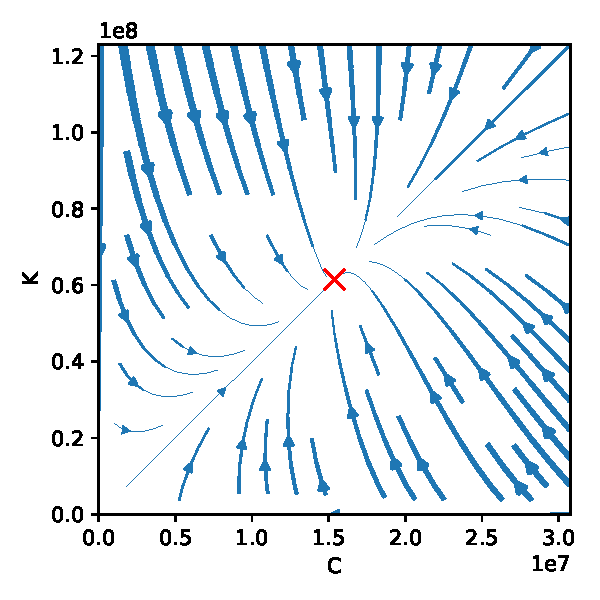
\includegraphics[width = .65 \textwidth]{./figures/phasespace.pdf}
        \caption[Phase space plot of a full clean economy]{Phase space plot of equations \eqref{eq:full_clean_ca1} and \eqref{eq:full_clean_ca2} \label{phase_space_plot}}
\end{wrapfigure}

To estimate the parameters of the model, I analyze some limiting cases of the system and compare them with real world timescales. , I can set reasonable values to some parameters.


\subsubsection{Full Clean Economy}
\label{sec:full_clean_economy}
Along the same lines, I can treat the case of a full clean economy (assuming that the fossil resource is depleted, or the households have for some other reason decided to only invest in clean capital $K_c$). \\
In this case, the equations for capital and knowledge accumulation are
\begin{subequations}
\begin{align}
    \dot{K}_c &= s b_c L^{\alpha} K_c^{\beta} C^\gamma - \delta K_c \label{eq:full_clean_ca1} \\
	\dot{C} &= b_c L^\alpha K_c^\beta C^\gamma - \chi C \label{eq:full_clean_ca2}
\end{align}
\end{subequations}
Assuming that $\alpha + \beta$ = 1, with equal elasticities for capital and labor e.g. $\alpha = \beta$, the stationary point of the system (except for the trivial one at $(0, 0)$ is 
\begin{equation}
  K_c^*= \left( \frac{\chi s}{\delta} \right) \left( \frac{s b_c^2 L}{\delta \chi} \right)^{\frac{1}{1-2\gamma}}, \qquad C^*\left( \frac{s b_c^2 L}{\delta \chi} \right)^{\frac{1}{1-2 \gamma}}
	\label{stationary_points}
\end{equation}
where the first one is non hyperbolic and the second one is stable which can be seen in the phase space plot in \cref{phase_space_plot} and the corresponding Jacobian
\begin{equation}
	J_{(K_c^*,C^*)} = 
		\begin{pmatrix}
			-\frac{1}{2}\delta & \gamma s \chi \\
			\frac{\delta}{2 s} & \chi \left(\gamma-1 \right)
		\end{pmatrix}
	\label{eq:learning_jacobian}
\end{equation}
whose Eigenvalues are strictly negative:
\begin{equation}
  \lambda_{1,2} = \frac{\delta}{2}(\gamma-1), \quad -\delta.
	\label{eq:learning_eigenvalues}
\end{equation}
The phase space plot in \cref{phase_space_plot} also suggests that there is a trajectory that satisfies 
\begin{equation}
	\frac{K_c(t)}{C(t)} = \frac{K^*_c}{C^*}
\end{equation}
meaning, one has to find a solution to the following ode:
\begin{equation}
	\dot{K}_c = s^{1-\frac{\gamma}{2}} b_c L_c^{\frac{1}{2}}K_c^{\frac{1}{2}(1-\gamma)} - \delta K_c
	\label{eq:learning_trajectory_ode}
\end{equation}
which can be done by means of separation of variables, resulting in
\begin{equation}
  K_c(t) = \left( s^{1-\frac{\gamma}{2}}\frac{b_c L^{\frac{1}{2}}}{\delta} + \exp\left[ (t_0-t) \frac{\delta (1-\gamma)}{2} \right] \right)^{\frac{2}{1-\gamma}}.
	\label{eq:learning_trajectory_solution}
\end{equation}
So, the system approaches its equilibrium approxitely exponentially from below, on a timescale that is given by
\begin{equation}
	t_c^* = \frac{2}{\delta(1-\gamma)}
	\label{eq_learning_equilibrium_timescale}.
\end{equation}
Assuming the same capital depreciation rate for clean capital as for dirty capital previously, together with $\gamma = 1/4$ which appears to be a fitting value according to \cite{Kahouli-Brahmi2008}, the timescale for clean capital accumulation is $t^*_c \approx 53 y$.

\subsubsection{Full on Dirty Economy}
\label{sec:full_dirty_economy}

Assuming, the fossil resources are very large, the dirty capital stock is significantly more profitable than the clean capital stock and subsequently all households decided to only invest in dirty capital. In this case I can treat the dirty sector isolated:
\begin{equation}
	\dot{K}_d = s I - \delta K_d, \quad I = w L + r_d K_d
	\label{eq:full_dirty_ca1}
\end{equation}
As shown before, $r_d$ is given by:
\begin{align}
	r &= \frac{\partial Y_d}{\partial K_d} - \frac{\partial c_R}{\partial K_d}, \quad c_R = b_R\left( \frac{G_0}{G} \right)^{2} R, \quad Y_d = eR, \\
	&\approx \left( 1-\frac{b_R}{e} \right)\frac{\partial Y_d}{\partial K_d},
	\label{eq:full_dirty_capital_rent}
\end{align}
and similarly for the wage $w$:
\begin{equation}
	w = \left( 1-\frac{b_R}{e} \right)\frac{\partial Y_d}{\partial L}.
	\label{eq:full_dirty_wage}
\end{equation}
So combining these, the income $I$ is equal to
\begin{equation}
	I = \left( 1-\frac{b_R}{e} \right)b_d (\alpha + \beta) L^{\alpha} K_d^{\beta}
	\label{eq_full_dirty_income}
\end{equation}
and using the assumption of zero profits e.g. $\alpha + \beta = 1$ the equation for capital accumulation \eqref{eq:full_dirty_ca1} reads
\begin{equation}
	\dot{K}_d = s\left( 1 - \frac{b_R}{e} \right) b_d L^{\alpha} K_d^{\beta} - \delta K_d
	\label{eq:full_dirty_ca2}
\end{equation}
This ordinary nonlinear differential equation can be solved by separation of variables.
\begin{equation}
  K_d (t) = K_d^{*} \left(1 - e^{(t_0-t)/t_d^{*}} \right)^{\frac{1}{\alpha}}
	\label{eq:dirty_capital_ac_solution}
\end{equation}
where the timescale for capital accumulation $t^*_d$ and the equilibrium dirty capital stock $K^*_d$ are
\begin{equation}
	t_d^{*} = \frac{1}{\alpha \delta}, \qquad K_d^{*} = \left( \frac{s b_d L^\alpha}{\delta}\left(1-\frac{b_R}{e}  \right) \right)^{\frac{1}{\alpha}}.
	\label{eq:full_dirty_capital_equilibrium_values}
\end{equation}
Since the capital depreciation rate $\delta$ is (at least for infrastructure) around 5\% p.a.\ and I assumed $\beta_d=1/2$ for the capital elasticity, the timescale for capital accumulation is $t^*_d \approx 40 y$.

\subsubsection{Fossil Resource Depletion}
\label{sec:resource_depletion}


\begin{wrapfigure}[15]{o}{.45 \textwidth}
    \vspace{-.8 cm}
    \hspace{-1.5cm}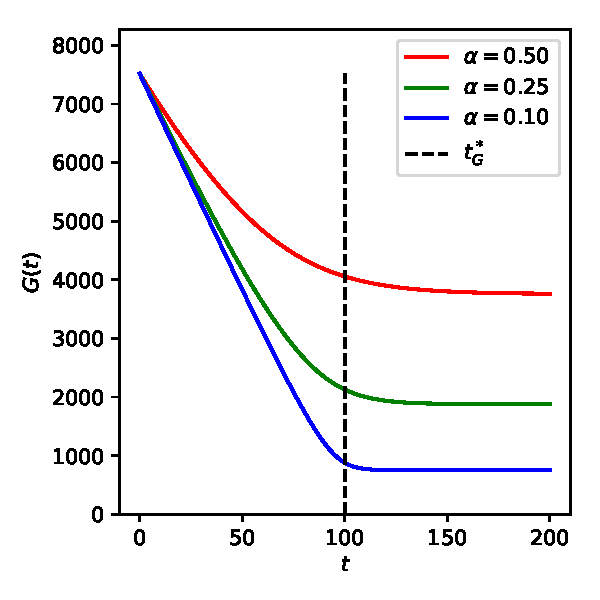
\includegraphics[width = .58 \textwidth]{figures/g_depletion.pdf}
    \caption[Resource depletion in a full dirty economy]{Resource depletion in a full dirty economy as described by eq. \eqref{eq:resource_deprec_approx}. The dashed line marks the approximate resource depletion time $t^*_G$. \label{fig:g_depletion}}
\end{wrapfigure}

For this analysis, I assume a full dirty economy like in \ref{sec:full_dirty_economy}. In addition, I assume that I can separate the timescales of resource depletion and dirty capital accumulation, e.g. I assume that dirty capital accumulation happens fast compared to fossil resource depletion such that I can approximate $K_d(t)$ with eq. \ref{eq:full_dirty_capital_equilibrium_values}. Consequently, the ode for fossil resource depletion is given by
\begin{align}
	\dot{G} &= -R \nonumber \\
        &= -\frac{b_d}{e}L^{\alpha}K_d^{*\ \beta_d} \nonumber \\
	&= - \frac{b_d}{e}L^{\alpha}\left(L^{\alpha} \frac{s}{\delta}b_d\left( 1-\frac{b_R}{e}\left( \frac{G_0}{G(t)} \right)^2 \right) \right)^{\frac{\beta_d}{1-\beta_d}}
	\label{eq:resource_deprec_approx}
\end{align}
This means that unsurprisingly, $G$ converges to a stable fix point $G^* = \sqrt{b_R/e}\ G_0$. Separating variables and substituting $g = G/G_0$ and $\varepsilon = \sqrt{b_R/e}$, the transient dynamic is given by
\begin{equation}
	\int_1^{g(t)} \frac{{\mathrm d} g'}{1 - \varepsilon^2/g'^2} = - \frac{s b_d^2 L}{e \delta G_0} \ t
	\label{eq:resource_transient_integral}
\end{equation}
To get a rough estimate of the time that it takes for the resource to deplete, I assume that $\varepsilon << 1$ and consequently for the most time, $\varepsilon^2/g'^2 << 1$.
This means that the integrand of the lhs.\ in eq.~\eqref{eq:resource_transient_integral} can be approximated by
\begin{equation}
	\int_1^{g(t)}1+\frac{\varepsilon^2}{g'^2} {\mathrm d}g' = \left[ g' - \frac{\varepsilon^2}{g'} \right]_1^{g(t)} = g(t) - \frac{\varepsilon^2}{g(t)} -1+\varepsilon^2.
	\label{eq:resource_transient_solution}
\end{equation}


This results in the implicit approximate solution:
\begin{equation}
  g(t) - \frac{\varepsilon^2}{g(t)} = 1 -\varepsilon^2 - \frac{s b_d^2 L}{e \delta G_0} \ t.
	\label{eq:resource_transient_solution2}
\end{equation}
According to this approximate solution, $g$ reaches $\alpha$ after a finite time $t^*_G$, which I use as the timescale for resource depletion:
\begin{equation}
	t^*_G = G_0\frac{e \delta}{s L b_d^2}\left( 1-\frac{b_R}{e} \right)
	\label{eq:resource_depletion_time}
\end{equation}
\Cref{fig:g_depletion} shows this resource depletion time in comparison to the numerical solution from eq. \ref{eq:resource_deprec_approx} for different values of $\alpha$ to give an impression of the goodness of the approximation.

There are different estimates for the depletion time of fossil resources ranging from approximately 60 years for crude oil to 100 years for gas and 200 years for coal.
So, I assume $t^*_G \approx 100y$. Using this, the initial resource stock $G_0$, the total population, the integrated world BIP (with an assumed growth rate of 2\%p.a.) I could get approximate estimates for $e$ and a relation of $b_d$ to  $b_R$.

% I use 2015 as the base year for my estimates. To estimate $e$ I use World GDP according to the World Bank database CITE ($75.037 \ 10^{12}$ \$) and world primary energy supply according to the BP statistical review of world energy ($13 \ 647$ Mtoe).
% Accordingly, $e$ is estimated at
% \begin{equation}
%   e \approx \frac{75.037 \; 10^{12} \; \$}{13.647 \; 10^9 \; \rm{toe}} = 5.5 \ 10^3 \left[ \frac{\$}{\rm{toe}} \right]
%   \label{ep:estimate_e}
% \end{equation}
\subsection{Parameter Values}
\label{sec:parameter_values}
\begin{sidewaystable}
	\centering
	\begin{tabular}{r|l|c|l}
          \makecell[l]{Symbol} & \makecell[l]{Default Value} & Unit & \makecell[l]{Parameter Description} \\\hline

                $\alpha_c$ & $2/3$ & & \multirow{3}{*}{\makecell[l]{Labor elasticities in the clean and dirty sector. \\Are assumed to be equal to allow for analytic \\calculation of labor shares between sectors}} \\ \hhline{---~}
                $\alpha_d$ & $2/3$ & & \\
                && & \\ \hline
                $\beta_c$ & $1-\alpha_c$ & & \multirow{2}{*}{\makecell[l]{Capital elasticities in the clean and dirty sector. Are fixed through the \\ assumption of no profits that is equivalent to $\alpha_i + \beta_i = 1$.}} \\ \hhline{---~}
                $\beta_d$ & $1-\alpha_d$ & & \\ \hline
                $\gamma$ & $1/8$ &  & Elasticity of knowledge in the clean sector.\\ \hline
                $L_1$ & $3.38 \cdot 10 ^{9}$ & billion people & Total labor in 2010. \\ \hline
                $\mu$ & 5.72 &  & \multirow{2}{*}{\makecell[l]{Exponents of resource usage $R$ and remaining \\resource stock $G$ in the resource extraction costs $c_R$. }} \\ \hhline{---~}
                 &  &  & \\ \hline
                $b_R$ & $184410.4 \cdot 10^{8}$ & \$/Mtoe & \multirow{3}{*}{\makecell[l]{Resource uptake efficiency and fossil usage efficiency for \\fossil resource. Together, they define the fraction of fossil \\resources that is not economically viable $G^* = G_0 \left(b_R/e^\rho\right)^{1/\mu}$.}} \\ \hhline{---~}
                $e$ & 4505 & \$/toe & \\
                & & & \\ \hline
                $G_0$ & $15.8 \cdot 10^5$ & Mtoe & \multirow{2}{*}{\makecell[l]{Initial and current fossil resource stock estimated from historical \\ data depicted in \cref{fig:historical_resource_use}.}}\\\hhline{---~}

                $G_1$ &  & Mtoe & \\ \hline
                $s$ & 0.25 & & Gross savings rate. \\ \hline
                $\delta $ & $5.6$ & \% p.a.  & \multirow{2}{*}{\makecell[l]{Capital depreciation rate. \\ Is assumed to be equal for both sectors}} \\
                &&\\ \hline
                $\tilde{b}_c$ &  $2.501 \cdot 10^{14}$ & U.S.\$ & \multirow{2}{*}{\makecell[l]{rescaled total factor productivity (TFP) in the clean and dirty sector. \\ as defined in eq. \ref{eq:rescalled_TFP_clean} and \ref{eq:rescalled_TFP_dirty}}} \\ \hhline{---~}
                $\tilde{b}_d$ & $5.175 \cdot 10^{14}$ & U.S. \$ & \\ \hline
                $K_{c1}$      & $2.04  \cdot 10^{15}$ & U.S. \$ & Estimated capital in the clean sector in 2010 \\ \hline
                $K_{d1}$      & $3.12  \cdot 10^{14}$ & U.S. \$ & Estimated capital in the dirty sector in 2010 \\ \hline
                $C_1$         & $7.8   \cdot 10^{14}$ & U.S. \$ & Estimated knowledge stock in the clean sector in 2010\\ \hline
                $\chi$ & 2 & \% p.a. & Knowledge depreciation rate \\ \hline
		$\tau$ & 1 & years & activity rate of households \\ \hline
		$\varphi$ & $1\leq\varphi\leq1$ & X & rewiring probability given an interaction event
	\end{tabular}
        \caption{Model parameters with description. Fitted to data from 1965 to 2010.}
	\label{tab:Heuristics_Parameter_list}
\end{sidewaystable}

To make the model results more intuitively accessible I roughly estimate the model parameters from real world data where possible. I chose 2010 as the base year, since for this year there are all the necessary estimates and data available. I do not intend to achieve any predictive accuracy with the model results and therefore use only very crude estimates for the model parameters. However, I believe that being able to express the model results at least in the right order of magnitude of real-world quantities makes also the qualitative results of the model easier to interpret.\\

First, I collect estimates for all parameters where there are values in the literature.\\

\textit{Input factor elasticities} are a defining set of parameters for Cobb-Douglas production functions. They measure the responsiveness of output with respect to a change in input factors. Historically, according to \cite{Douglas1976} the values for $\alpha$ range between approximately 0.5 and 0.75. For simplicity, I set $\alpha=2/3$ which however does not limit the generality of the approximate solutions that are developed later in section \ref{sec:Approximation} ff. \cite{Douglas1976} also states that $\alpha+\beta=1$ is a fair approximation of the actual data.
\begin{wrapfigure}[21]{o}{.55 \textwidth}
	\vspace{-.4 cm}
        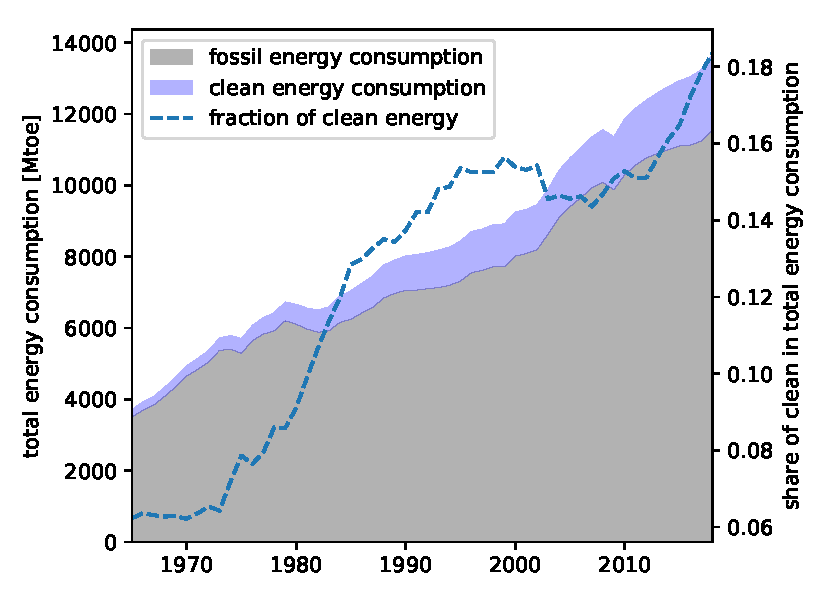
\includegraphics[width = .65 \textwidth]{./figures/energy_consumption_clean_dirty.pdf}
        \caption[Data for world energy use devided into dirty and clean sources.]{Energy usage divided into dirty (coal, oil, gas) and clean (hydro, nuclear, other renewables). The dashed line indicates the fraction of clean energy consumption. Data from \cite{dudley2019bp}.\label{fig:energy_data}}
\end{wrapfigure}
\textit{Elasticity of knowledge $\gamma$} is also the rate of learning of technology in the clean sector as discussed in \ref{sec:model_description}. This heavily depends on the technology under consideration. According to \cite{Kahouli-Brahmi2008} estimates for learning-by-doing rates approximately range between 10\% and 20\%. As an approximate value, I set $\gamma=1/8$. \\
\textit{The savings rate $s$} indicates the fraction of income that households save on average. I use a fixed savings rate for all households that is set to $s=0.25$ which is roughly in line with data for OECD countries\footnote{see \url{https://data.worldbank.org/indicator/NY.GNS.ICTR.ZS}}.\\
\textit{Total labor $L$} is taken from world bank data\footnote{see \url{https://data.worldbank.org/indicator/SL.TLF.TOTL.IN}} which estimates it at 3.38 billion people for 2016.\\
Second, I estimate parameters for which this can be done with a back-of-the-envelope calculation.\\
\textit{The knowledge depreciation rate $\chi$ in the clean sector} is assumed to be primarily a human capital effect. Therefore, I approximate the rate of knowledge depreciation with the rate workers leaving the workforce which assuming a typical career length of ~45 years results in roughly $\chi=0.02$. \\
\textit{The energy intensity in the dirty sector $e$} is estimated from world GDP\footnote{according to \url{https://data.worldbank.org/indicator/NY.GDP.MKTP.CD} world GDP was ~ $5.35 \cdot 10^{14}$ U.S. \$ for the year 2010} and the consumption of fossil ($R$) and renewable ($E$) energy\footnote{both values are taken from the BP statistical review of world energy \cite{dudley2019bp}. I count the consumption of energy from Oil, Coal and Gas as fossil and everything else as renewable.} as follows. I approximate the fraction of total economic output coming from the clean sector as the fraction of fossil energy production and estimate the energy intensity $e$ as $Y_d/R$ for the base year 2010:
\begin{equation}
  e = \frac{Y_d}{R} \approx \frac{GDP \frac{R}{R+E}}{R} = \frac{GDP}{R+E} \approx \frac{5.3 10^{14} \$}{11.9 10^9 \mathrm{toe}} = 4505 \frac{\$}{\mathrm{toe}}
  \label{eq:energy_intensity_estimate}
\end{equation}

\textit{I approximate the capital stocks in the clean and dirty sector} by assuming that the relative output of both sectors is equal to the relative consumption of fossil and renewable energy e.g. $Y_c/Y_d = E/R$. Additionally, I assume that for my purpose, national income can be sufficiently well approximated by gross production and that the capital income ratio\footnote{The capital income ration is estimated as the sum over national income by all countries divided by the estimated sum of private and national capital over all countries. For details on data and methodology, see \cite{piketty2014technical}} (CIR) of 440 \% for the year 2010 estimated by \cite{piketty2014} for the economy as a whole can be used to approximate the capital stocks of each sector individually.

\begin{equation}
  K_d \approx CIR \cdot Y_d \approx CIR \cdot GDP \cdot \frac{R}{E + R} \approx 2.04 \cdot 10^{15} ~ \textrm{U.S.} \$
  \label{eq:approx_dirty_capital}
\end{equation}

and 
\begin{equation}
  K_c \approx CIR \cdot Y_c \approx CIR \cdot GDP \cdot \frac{E}{E + R} \approx 3.12 \cdot 10^{14} ~ \textrm{U.S.} \$
  \label{eq:approx_clean_capital}
\end{equation}
\textit{The capital depreciation rate $\delta$} is assumed to be equal in both sectors. Capital depreciation rates strongly depend on the type of capital under consideration. Typical estimates range from 1.5 \% to 8.5\% for different kinds of capital see \cite{Kamps2005} and \cite{Gupta2014}. This leaves some freedom to chose $\delta$. I use this to set $\delta$ such that the estimated total capital stock $K = K_c + K_d$ together with the chosen savings rate of $s=0.25$ is an equilibrium solution to 
\begin{equation}
  \dot{K} = s \cdot Y - \delta K
  \label{eq:delta_estimate}
\end{equation} 
which results in a depreciation rate of $\delta\approx 5.68 \% \mathrm{p.a.}$.\\

\textit{I estimate the initial value of the knowledge stock in the clean sector $C$} for the base year from the time series of production in the clean sector. Production in the clean sector is approximated equivalently to eq. \ref{eq:energy_intensity_estimate} as world GDP times the fraction of clean energy consumption for the years of 1965-2010. I use the discrete version of \eqref{eq:learning_by_doing}:
\begin{equation} 
  C(t+1) = (1-\chi)C(t) + Y_c(t)
  \label{eq:discrete_clean_knowledge}
\end{equation}

to approximate the knowledge stock for the year 2010 as $C \approx 7.8 \cdot 10^{14}$ U.S. \$. \\
I estimate \textit{the initial fossil resource stock $G_0$ and the current resource stock $G$} for the base year from the historical usage of fossil fuels (after 1965 for which I have the data depicted in \cref{fig:historical_resource_use}) and the current estimates of fossil fuels remaining according to current use. 

There are different estimates for the depletion time of fossil resources ranging from approximately 60 years for crude oil to 100 years for gas and 200 years for coal.\\ As the model does not differentiate between different types of fossil resources, I use a depletion time of 100 years and approximate the current resource stock as the depletion time times the current fossil resource use:

\begin{align} 
  G(t=2010) 
  &\approx R(t=2010) \cdot 100, \nonumber \\
  &= 11.6 \cdot 10^{5} ~ \mathrm{Mtoe},
  \label{eq:current_fossil_resource_stock}
\end{align}
and the initial fossil resource stock as the current fossil resource stock plus the estimated cumulative resource stock according to the extrapolated fossil resource use depicted in \cref{fig:historical_resource_use}:
\begin{equation} 
  G_0 \approx G(t=2010) + \sum_{t=1965}^{2010} R(t) = 15.5 \cdot 10^{5} ~ \mathrm{Mtoe}.
  \label{eq:initial_fossil_resource_approximation}
\end{equation}
\begin{wrapfigure}[22]{o}{.55 \textwidth}
	%\vspace{-.4 cm}
        %\hspace{-1.5 cm}
        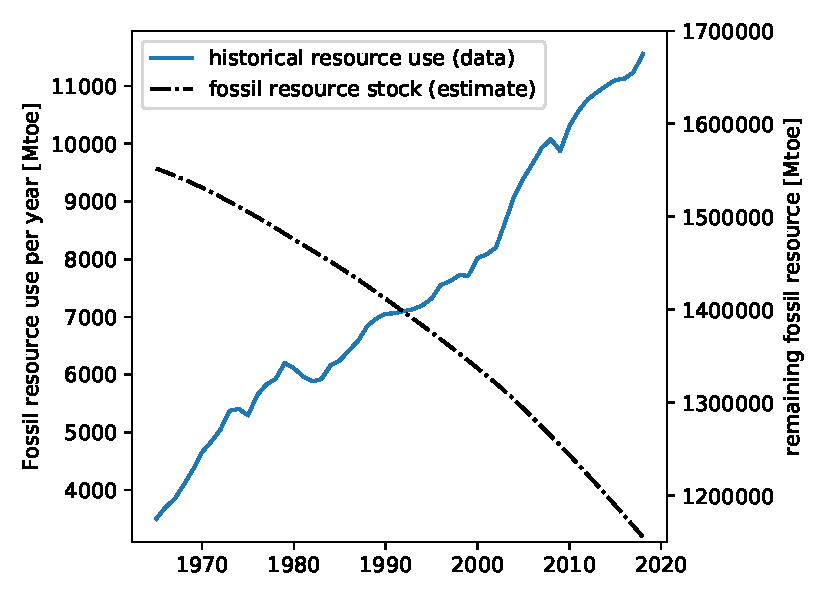
\includegraphics[width = .68 \textwidth]{./figures/fossil_resource_per_year.pdf}
        \caption[Historical data of fossil resources]{Historical data of fossil resources (coal, oil and gas) for the years 1965-2018 according to \cite{dudley2019bp} and estimated historical fossil resource stock according to eq. \ref{eq:current_fossil_resource_stock} and \ref{eq:fossil_resource_time_series}. \label{fig:historical_resource_use}}
\end{wrapfigure}

Finally, I estimate the set of remaining parameters $b_R$, $\mu$, $b_c$ and $b_d$ as follows:

I estimate the parameters of the fossil resource cost function $b_R$ and $\mu$ from historical energy price and fossil resource consumption data. I use the historical oil price\footnote{I use the yearly average oil price for different types of crude oil according to \url{https://www.statista.com/statistics/262858/change-in-opec-crude-oil-prices-since-1960/}} as proxy for the fossil resource price $p_R$ as historical data for prices for different types of fossil energy sources \citep{owidfossilfuels} shows that prices are strongly correlated and of the same order of magnitude. I create a time series of the fossil resource stock $G(t)$ from $G_0$ as estimated in eq. \ref{eq:initial_fossil_resource_approximation} and the time series of fossil resource use in \cref{fig:historical_resource_use} like

\begin{equation} 
  G(t) = G_0 - \sum_{t=1948}^{t}R(t),
  \label{eq:fossil_resource_time_series}
\end{equation}

I approximate the yearly cost of fossil resource as the product of the approximate resource price times the yearly resource use: $c_R(t) \approx p_R(t) \cdot R(t)$. 
\begin{wrapfigure}[19]{o}{.55 \textwidth}
	\vspace{-.4 cm}
        \hspace{-1.25 cm}
        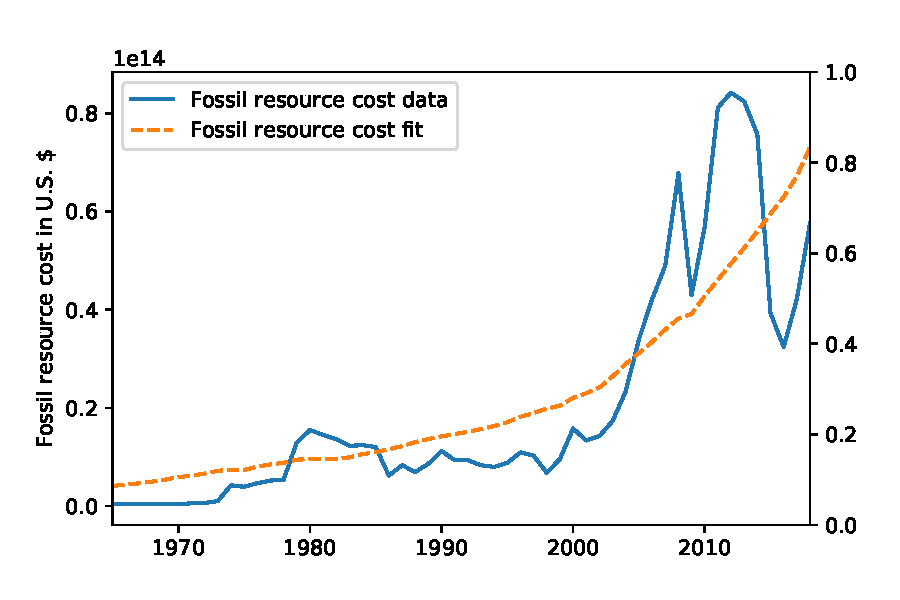
\includegraphics[width = .67 \textwidth]{./figures/resource_price_fit.pdf}
        \caption[Fit of model resource cost function to historical data]{Fit of resource cost according to eq. \ref{eq:resource_cost} to historical data generated from fossil resource use and yearly average crude oil prices as approximate fossil resource price. \label{fig:resource_cost_fit}}
\end{wrapfigure}
Then I use least squares to fit resource cost eq. \ref{eq:resource_cost} as a function of the data for resource use $R(t)$ and remaining resource $G(t)$ to the estimate data for the total resource cost $c_R(t)$ which results in 
\begin{align}
  &b_R \approx 10.4 \cdot 10^{8} \frac{\$}{\mathrm{Mtoe}} ~ \mathrm{and}\\
  & \mu \approx 5.72.
  \label{eq:estimate_resource_cost}
\end{align}
The resulting fit is given in \cref{fig:resource_cost_fit}.

To estimate the total factor productivities in the clean and dirty sector $b_c$ and $b_d$, I use equations \ref{eq:clean_production} and \ref{eq:dirty_production} and plug in the solutions for the labor shares $L_c$ and $L_d$ from equations \ref{eq:clean_labor} and \ref{eq:dirty_labor} as well as the estimates for $K_c$, $K_f$, $\alpha$, $\beta$, $\gamma$, $s$, $\delta$, $\chi$, $e$, $C$, $G0$, $G$, $b_R$, $\mu$ and the data for $R$ and $L$. Then, I can set them equal to the estimates for $Y_c$ and $Y_d$ to obtain an implicit condition for $b_c$ and $b_d$. Using numerical root finding, this results in 
 \begin{align}
  &b_c \approx 22.94 ~ \mathrm{people} ^{-\alpha} ~ \mathrm{U.S. \$}^{1-\beta-\gamma} \quad \mathrm{and} \\
  &b_d \approx 1844 ~ \mathrm{people}^{-\alpha} ~ \mathrm{U.S. \$}^{1-\beta}.
  \label{eq:estimate_total_factor_productivities}
\end{align}

Now, if you think that these units look weird, you are not alone. There is an ongoing debate between economists about sound ways to interpret total factor productivity with regards -- but not limited to -- their units. Up to the point that e.g. \cite{Barnett2007} goes so far as to state that there is no other way as to regard them in their current formulation as ``either meaningless or economically unreasonable''. Official statistics usually bypass this problem insofar as they avoid measuring levels but construct unitless growth rates for the outputs and inputs and therefore also for the residual. Inspired by this practice I will do a similar trick. I rescale the total factor productivity by dividing the input variables by typical yet arbitrarily chosen values:
\begin{align}
  Y_c &= \tilde{b}_c \left( \frac{L_c}{L_0} \right)^{\alpha} \left( \frac{K_c}{K_{c0}} \right)^{\beta} \left( \frac{C}{C_0} \right)^{\gamma} \label{eq:rescalled_TFP_clean} \\
  Y_d &= \tilde{b}_d \left( \frac{L_d}{L_0} \right)^{\alpha} \left( \frac{K_d}{K_{d0}} \right)^{\beta}. \label{eq:rescalled_TFP_dirty}
\end{align}
This brings a number of advantages. First, the rescaled total factor productivities $\tilde{b}_c$ and $\tilde{b}_d$ are measured in the same units as economic output, thereby avoiding the weird physical units from above. Second, the rescaled TFPs are independent of the input factor elasticities $\alpha$, $\beta$ and $\gamma$.
To rescale the TFPs, I will use the values of labor, capital and knowledge for the base year of the previous estimates. This results in
\begin{align} 
  &\tilde{b}_c = b_c L_0^{\alpha}K_{c0}^\beta C_0^{\gamma} = 2.501 \cdot 10^{14} ~ \mathrm{U.S. \$}, \\
  &\tilde{b}_d = b_d L_0^{\alpha}K_{d0}^\beta =              5.175 \cdot 10^{14} ~ \mathrm{U.S. \$}.
  \label{eq:rescalled_TFP_values}
\end{align}
Note, that these estimates for $\tilde{b}_c$ and $\tilde{b}_d$ can only be used in combination with the values of labor, capital and knowledge for the base year $L_0$, $K_{c}$, $K_{d0}$ and $C_0$. However, this has the advantage that these values can be changed independently from the estimates. This is very useful once I want to change the values of e.g. input factor elasticities such as the rate of learning-by-doing to evaluate their influence on the qualitative behavior of the model.\\

The parameter values that were estimated in this chapter are the foundation on which the following model analysis can be interpreted in terms of real economic quantities which hopefully helps to evaluate the findings intuitively in a sociopolitical and economic context of the twenty first century.
Still, both the model and the parameter estimates are obviously oversimplified for exact quantitative predictions but quantitative predictions were never the goal of the model.

\iffalse
\subsubsection{Opinion spreading in the adaptive voter model}
A common way to describe the dynamics of the adaptive voter model in terms of macroscopic variables is the pair approximation.
For simplicity, lets assume a system with two possible opinions $A$ and $B$, on a network with $N$ nodes and $K$ edges.
I describe the model using a vector $(x, y, z)^T$:
\begin{equation}
	x = \frac{[A]-[B]}{N}, \quad y = \frac{[AA]-[BB]}{K}, \quad z = \frac{[AB]}{K}
	\label{avm_variables}
\end{equation}
There are four possible events in the system
\begin{itemize}
	\item 1. an A node rewiring,
	\item 2. a B node rewiring,
	\item 3. an A node adapting a B node and 
	\item 4. a B node adapting an A node.
\end{itemize}
The probabilities for these events to happen are
\begin{align}
	p_1 &= \varphi\frac{z(1+x)}{2(1+y)}, \quad p_2 = \varphi \frac{z (1-x)}{2(1-y)} \\
	p_3 &= (1-\varphi)\frac{z(1+x)}{2(1+y)}1/2({\mathrm tanh}(\Delta I)-1),\\
	p_4 &= (1-\varphi)\frac{z(1-x)}{2(1-y)}1/2({\mathrm tanh}(-\Delta I)-1)
	\label{avm_event_ps}
\end{align}
and their influence on the state vector $s = (x, y, z)^T$ are $s' = s + s_i$ with $s_i$ one of the following:
\begin{align}
	s_1 &= \colvec{3}{0}{1}{-1}, \quad s_3 = \colvec{3}{-2}{-2k\frac{1+y}{1+x}}{-1+2k\frac{1-y-2z}{1-x}-\frac{1-y-2z}{1-y}}\\ 
	s_2 &= \colvec{3}{0}{-1}{-1}, \quad s_4 = \colvec{3}{2}{2k\frac{1+y}{1+x}}{-1+2k\frac{1-y-2z}{1-x}+\frac{1-y-2z}{1-y}}
	\label{avm_event_effects}
\end{align}
Such that in the limit for large N, one gets deterministic equations for $x$, $y$ and $z$:
\begin{align}
	\frac{\dot{x}}{\tau} =& -(1-\varphi)\frac{z}{2}\frac{1-x}{1-y}(\mathrm{ tanh}(\Delta I)-1) + (1-\varphi)\frac{z}{2}\frac{1+x}{1+y}(\mathrm{ tanh}(-\Delta I)-1) \\
\frac{\dot{y}}{\tau} =& \quad \varphi\frac{z}{2}\left( \frac{1+x}{1+y} + \frac{1-x}{1-y} \right) + (1-\varphi)kz\left( \mathrm{ tanh}(-\Delta I) - \mathrm{ tanh}(\Delta I) \right) \\
	\frac{\dot{z}}{\tau} =& -\varphi\frac{z}{2}\left( \frac{1+x}{1+y} + \frac{1-x}{1-y} \right) \nonumber \\
	& + (1-\varphi)\frac{z}{2} \left[ \frac{1+x}{1+y} \frac{1}{2}(\mathrm{ tanh}(\Delta I)-1) \left( (1+y-2z)\left( \frac{2k}{1+x}-\frac{1}{1+y} \right)-1 \right) \right. \nonumber \\
	& \hspace{1.9 cm} + \left.\frac{1-x}{1-y}\frac{1}{2}(\mathrm{ tanh}(-\Delta I)-1)\left( (1-y-2z)\left( \frac{2k}{1-x}-\frac{1}{1-y} \right)-1 \right)  \right]
	\label{avm_ode}
\end{align}
assuming that the income difference $\Delta I$ between different cue orders is sufficiently large, this can be reduced to
\begin{align}
	\frac{\dot{x}}{\tau} =& -(1-\varphi)\frac{z}{2}\frac{1-x}{1-y} \\
\frac{\dot{y}}{\tau} =& \quad \varphi\frac{z}{2}\left( \frac{1+x}{1+y} + \frac{1-x}{1-y} \right) + (1-\varphi)kz \\
	\frac{\dot{z}}{\tau} =& -\varphi\frac{z}{2}\left( \frac{1+x}{1+y} + \frac{1-x}{1-y} \right) \nonumber \\
	& + (1-\varphi)\frac{z}{2} \left[ \frac{1+x}{1+y} \left( (1+y-2z)\left( \frac{2k}{1+x}-\frac{1}{1+y} \right)-1 \right) \right]
	\label{avm_ode_reduced}
\end{align}
and from this one can see that the timescale for $x$ to reach its equilibrium values is roughly 
\begin{equation}
	t_a^* = \tau(1-\varphi)
	\label{avm_timescale}
\end{equation}
Since, at least according to my impression, people don't really change their minds or make new friends too often, I propose keeping this timescale between $1<t_a^*<10$ years.
\fi
\newpage
\subsection{Opinion formation and decision making}
\label{sec:oppinion_formation_and_decision_making}

I assume that households use the Take-the-Best heuristic as explained in section~\ref{sec:intro_bounded_rationality} to decide whether to invest their savings in the clean or the dirty sector. This assumption results in three follow up questions that have to be answered for the model setup. A) Which cues i.e. bits of information to the households use to compare the two sectors for their decision? B) Which combinations of these cues (i.e. which cue orders) do I want to model? C) Which initial distribution of cue orders should I use as an initial condition. This chapter will answer these three questions in this order.

To represent the cue order in the model and in this text, I assign numbers to the different cues $(c_l)$ and represent cue orders $O$ as lists of these numbers: $O: (c_l,\dots c_m)$. As a rule, cues only appear once in each cue order and if one cue definitively discriminates between options, there will be no other cues after it.

\subsubsection*{A) Which information do households use to compare the clean and the dirty sector for their investment decision?}
I assume that households use information that is available to them either in their own mind such as inherent norms and preferences as well as information that is available to them in their surroundings such as factual data about their economic performance of the clean and the dirty sector or the behaviour of their acquaintances.\\

\textit{Inherent norms:}
I assume that it is an option for households to invest in one or the other sector purely out of their inherent conviction to do so, disregarding all other information that might be available. This constitutes two cues: 
\begin{itemize}
  \item [ $(0)$ ] the household invests its savings in the clean sector, regardless of all other information,
  \item [ $(1)$ ] the household invests its savings in the dirty sector, regardless of all other information.
\end{itemize}
Both of these cues definitively discriminate between the two sectors.\\

\textit{Factual data about the economic performance of the clean and the dirty sector:}
Many behavioral investment models such as \cite{Lux1999}, \cite{Alfarano2008a}, \cite{Chiarella2011a} and \cite{Hommes2017BoomsPrices} assume two possible ways to make investment decisions and hence model two types of investors - for an overview see e.g. \cite{Hommes2006a} or \cite{Chakraborti2011}. Such models usually assume that investors either invest based on their beliefs about an inherent value of an investment (such investors are called fundamentalists as they believe in an inherent fundamental value of an asset and that the asset price will return to this value eventually) or based on their beliefs on a future value of an investment (such investors are called chartists as they do believe that asset prices are inherently volatile and that their future price can best be read out out of the price time series - the chart).
Motivated by this approach, I assume that households can use either the current value of an investment to ground their decision or they can use an estimate about which of the investments will be more valuable in the future. I also assume that they use the current return rates $r_c$ and $r_d$ as a proxy for the inherent value of an investment in the clean or the dirty sector and that they use their first derivatives with respect to time $\dot{r}_c$ and $\dot{r}_d$ as a proxy for the future development of the value of an investment in one or the other sector. I implement these as the two following cues:
\begin{itemize}
  \item [$(2)$] households invest in the sector whose capital return rate is distinctly higher e.g. $r_j > (1+\iota) r_k$,
  \item [$(3)$] households invest in the sector whose trend in capital return rates is distinctly more positive e.g. $\dot{r}_k > (1+\iota) r_k$,
\end{itemize}
and with distinctly, I mean $\iota = 0.1$.\\

\textit{Behavior of households' acquaintances:}
As discussed previously in section \ref{sec:investment_decision_making}, I assume that one of the households different drivers is homophily, i.e. the desire to be similar to ones acquaintances. I have already used this in the motivation of the social learning component where households are homophilic with regards to their beliefs that are represented by their cue orders. To be consistent, I use it again here where I say that one possible driver for households investment decision is that they want to behave similar to their acquaintances. This behavior is also referred to as `Imitate the Majority' in the heuristic decision making literature see e.g. \cite{Gigerenzer2009} \cite{garcia2009does} and \cite{Gigerenzer2011}. 
I implement this in terms of the following cue:
\begin{itemize}
  \item [$(4)$] A household invests its savings in the sector in which the majority of its acquaintances invest e.g. it invests in the sector $k$ if $\sigma_k > 0.5 + \iota$
\end{itemize}
with $\sigma_k$ being the fraction of acquaintances investing in sector $k$ and again $\iota=0.1$.

\subsubsection*{B) Which cue orders to consider in the model?}
With regards to the cue orders in the model, there is a trade off to consider. For a high number of cue orders, one needs a considerably higher number of households to get enough households to use each cue order to get meaningful results in terms of statistics. But a higher number of households leads to significantly more costly numerical simulations. (For a short study of model run times in its current implementation depending on the number of simulated households, see \cref{fig:runtime}.) Therefore, I will not consider all possible cue orders\footnote{All possible combinations would be $5!=120$, however since cues 0 and 1 end the heuristic, only $38$ of these cue orders are distinct.}, but I will restrict the model to cue orders of length two\footnote{I hypothicise that only a vanishing fraction of decisions would be made with more than two cues and that making these decisions at random (as the TTP Heuristic prescribes it) instead of with more cues does not make a difference. I could track the fraction of decisions that are made at random for an ensemble of simulations at some point to prove this.}. Additionally, of all $14$ remaining possible cue orders of length $2$, I only consider a subset. This subset must still represents all possible cues and should therefore be sufficient to answer the question of how different possible grounds for an investments
\begin{wrapfigure}[23]{o}{.4 \textwidth}
	\vspace{-.4 cm}
        \hspace{-1.9 cm}
        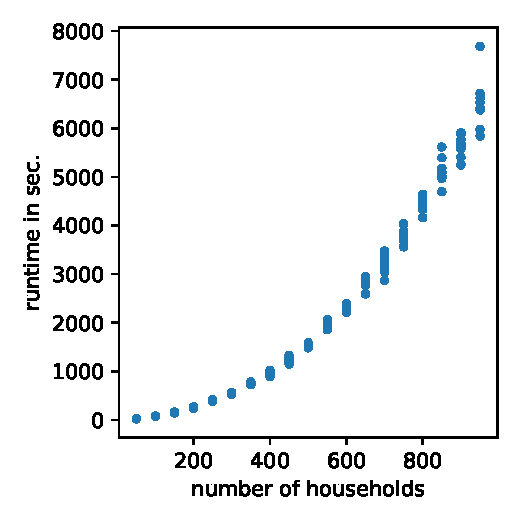
\includegraphics[width = .55 \textwidth]{./figures/runtime.pdf}
        \caption[Model run time depending on number of households]{Run times of the model in my implementation (Python) depending on the number of households modelled.\label{fig:runtime}}
\end{wrapfigure}
decision that are prevalent in the population influence the aggregate behavior of the social-economic system with regards to a possible rapid decarbonization transition.\\

Overall, I consider three different types of households. First, households that ground their decisions based on financial incentives e.g. that consider cues $(2)$ and $(3)$ in different order. Second, I consider households that ground their investment decision on homophily, but fall back to other discriminating information, if there is no clear majority amongst their acquaintances e.g. they use cue $(4)$ first and one of the other cues second. Finally, I consider households that invest in one or the other sector out of an inherent preference, e.g. they use cue $(0)$ or $(1)$ and no other cues, since these cues are always decisive. \\

To sum up, I consider the following set of eight cue orders and for a more intuitive description also the following names for the households using them:
\begin{itemize}
  \item [$(2, 3)$]: myopic investor,
	\item [$(3, 2)$]: trend sensitive investor,
	\item [$(4, 2)$]: myopic herder,
	\item [$(4, 3)$]: trend sensitive herder,
	\item [$(4, 1)$]: Green conformer,
	\item [$(4, 0)$]: Conservative conformer,
	\item [$(1)$]: `Gutmensch',
	\item [$(0)$]: Redneck
\end{itemize}
With this set of cue orders, the remaining question is their frequency among the population of households.

\subsubsection*{C) Which initial distribution of cue orders should be used?}

The initial condition for the heterogeneous households consists of the distribution of cue orders, the distribution of the different kinds of capital and the configuration of the acquaintance network. This determines the investment decisions of the individual households and consequently the fraction of savings that is invested in the two economic sectors. \\
Arguably, to yield realistic results, the initial fraction of savings that goes into the two economic sectors should be consistent with the economic situation and historical data that the parameters of the economic model were fitted to. On the one hand, considering this situation, there is no actual data on the relative shares of investment. However, since I chose the parameters such that the total capital stock is in equilibrium subject to investment and depreciation according to eq. \ref{eq:delta_estimate}, it is sufficiently close to require that the relative shares of the capital stocks in the two sectors $K_c(t)/K_d(t)$ remains approximately constant.\\

\begin{figure}[t]
  \centering
  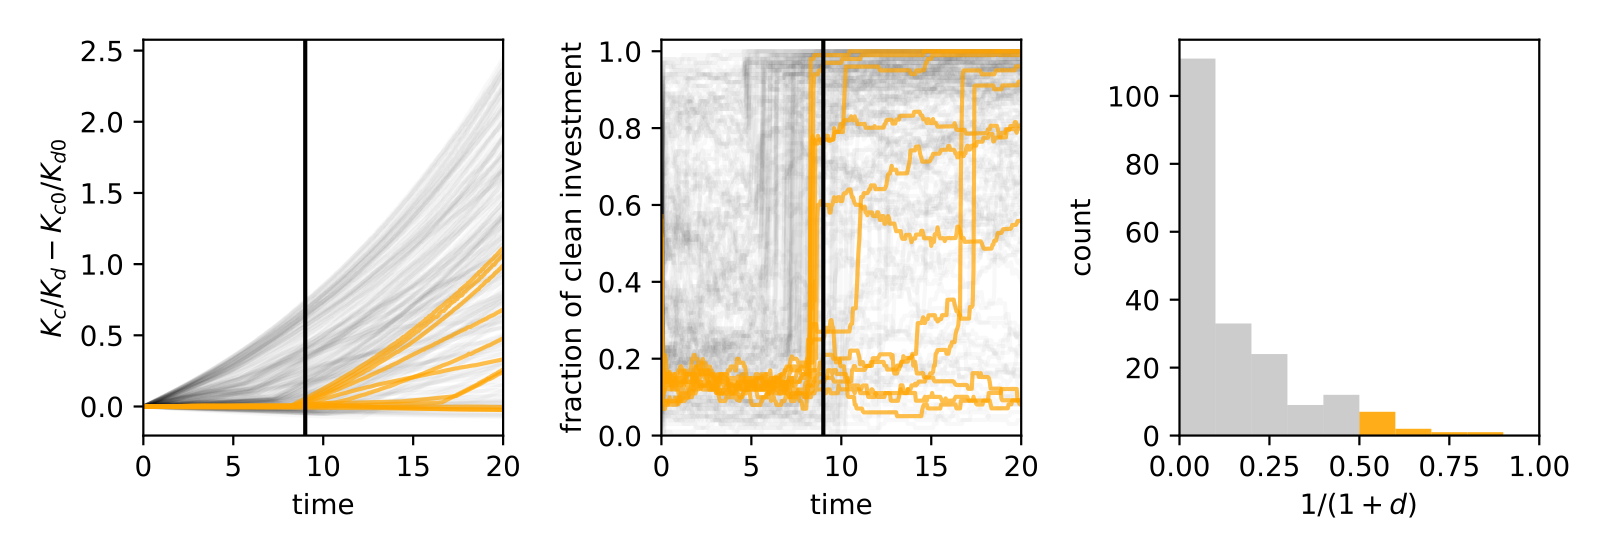
\includegraphics[width= \textwidth]{figures/initial_condition_sampling.png}
  \caption[Trajectories of N=200 runs with initial conditions for cue orders sampled from an uninformed prior]{\textbf{Trajectories of N=200 runs with initial distribution of cue orders sampled from an uninformed prior.} Panel a shows the distance of the simulated relative shares of capital $K_c(t)/K_d(t)$ from the initial condition. Panel b shows the fraction of total investment going into the capital stock of the clean sector. Panel c shows the distribution of closeness as defined by eq. \ref{eq:distance_criterion} and eq. \ref{eq:closeness} for the simulated trajectories.}
  \label{fig:initial_conditions_sampled}
\end{figure}
Therefore, I want to find an initial distribution of cue orders that likely leads to an aggregate ration of clean and dirty investment that keeps the ration of capital in the two sectors constant.\\

To find an initial distribution of cue orders that is likely to fulfill this criterion of an approximately constant ratio of capital in the two sectors, I use a method that is loosely inspired by Bayesian updating. Put simply, I first sample the initial distribution of cue orders from an uniformed prior then second, simulate the resulting model trajectory and calculate its distance $d$ to the formalized criterion and third, I calculate the weighted sum over the sample of initial cue order distributions using the inverse of the distance as weight to use it as the actual initial condition.



More precisely, I define the initial distribution of the 8 different cue orders by their relative frequencies $Q: [n_1, \cdots n_8]$ among the households. Given a fixed number of households $H$, the set of possible cue order distributions is equal to the discrete points on the 7 dimensional hyperplane that is given through $H = \sum_i n_i, n_i \in \mathbf{N^{+}}$. To get an equally distributed sample of these points $Q_m$, I use a Dirichlet distribution $\mathrm{Dir}(\mathbf{\alpha})$ with $\mathbf{\alpha}=(\alpha_1, \cdots \alpha_8), ~ \alpha_i=1$. I then randomly assign a cue order to each households according to their frequencies as given by $Q_m$. I also randomly assign equal shares of either clean or dirty capital each household - independent from their assigned cue order. Finally, I use an Erd\H{o}s-Renyi random graph with $p=0.1$ as the initial acquaintance network between households where acquaintance relations are set independent of the households' cue orders.


\begin{table}[t]
    \centering
    \begin{tabular}{c|c|l}
        Relative frequency & Cue order & Name \\ \hline
        $0.145$&$(2, 3)~$&myopic investor\\
    $0.075$& $(3, 2)~$& trend sensitive investor\\
        $0.124$& $(4, 2)~$& myopic herder\\
        $0.118$& $(4, 3)~$& trend sensitive herder\\
        $0.139$& $(4, 1)~$& Green conformer\\
        $0.166$& $(4, 0)~$& Conservative conformer\\
        $0.074$& $(1)~$& `Gutmensch'\\
        $0.158$& $(0)~$& Redneck

    \end{tabular}
    \caption{Fitted initial cue order distribution in terms of relative frequencies.}
    \label{tab:initial_cue_order_dist}
\end{table}

For these initial conditions, I simulate model trajectories for the years 2010-2030. For these trajectories, I calculate the distance to the chosen criterion of constant relative capital stocks between the sectors as as the Euclidean distance for the years 2010-2019:
\begin{equation}
  d_m = \sqrt{\sum_{t=2010}^{2019}\left( \frac{K_c(2010)}{K_d(2010)} - \frac{K_{c,m}(t)}{K_{d,m}(t)} \right)^{2}}.
  \label{eq:distance_criterion}
\end{equation}
I chose the years 2010-2019, as I would argue that looking back at the last decade, a major decarbonization transition is yet to come.
\Cref{fig:initial_conditions_sampled} a) shows the relative shares of capital for a sample of $M=200$ initial cue order distributions $Q_m$ with the one that can be considered close to the desired criterion highlighted in orange. In quantitative therms, I define closeness $cl$ as
\begin{equation}
  cl = \frac{1}{1+d}
  \label{eq:closeness}
\end{equation}
and consider a trajectory to be close if $cl > 0.5$.
The resulting initial distribution of cue orders $Q_r$ that hopefully fulfills the desired criterion is then calculated as
\begin{equation}
    Q_r = \frac{1}{\sum_m \frac{1}{d_m}}\sum_{m}\frac{1}{d_m} Q_m.
  \label{eq:updated_cue_order_distribution}
\end{equation}
The resulting cue order distribution is given in table \ref{tab:initial_cue_order_dist}.
Note that this only sets the relative frequencies of cue orders and does not determine the microscopic configuration of acquaintance relations, initial capital distribution and individual cue order assignment.

\begin{figure}[t]
  \centering
  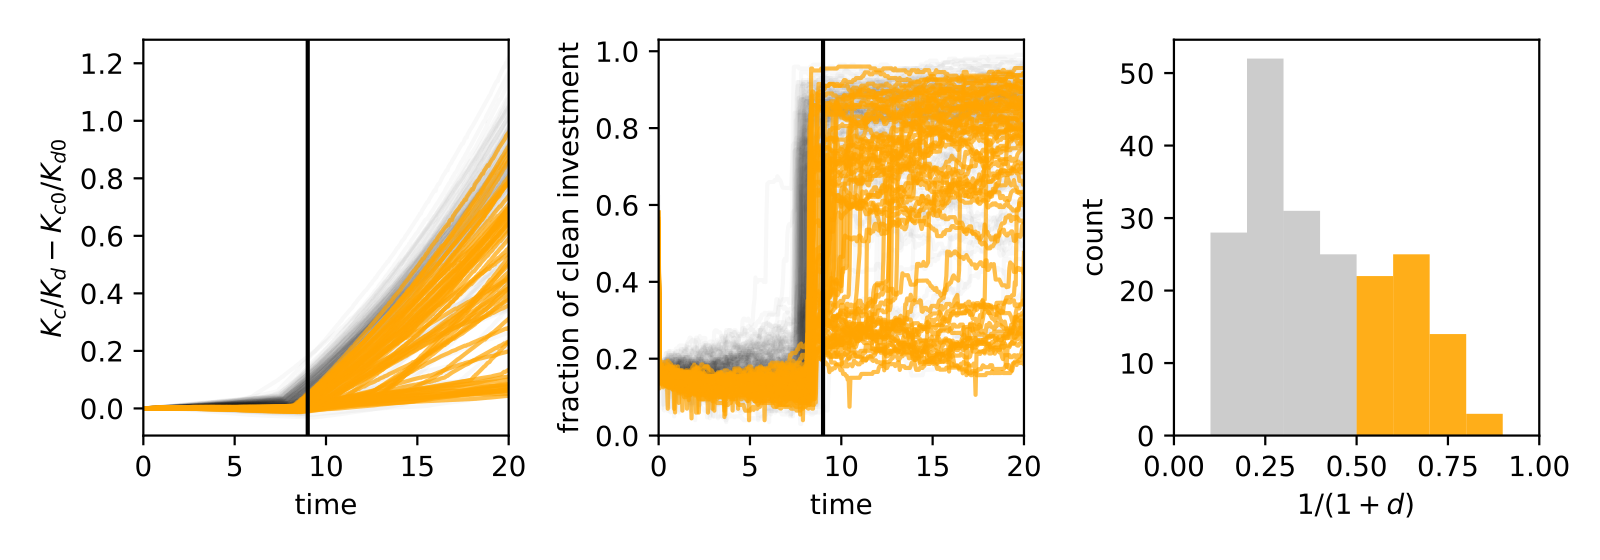
\includegraphics[width= \textwidth]{figures/initial_condition_fitted.png}
  \caption[Trajectories of N=200 runs with updated initial conditions]{\textbf{Trajectories of N=200 runs with updated initial conditions.} Initial relative frequencies of cue orders are calculated as to the weighted sum of the initial relative frequencies in \cref{fig:initial_conditions_sampled}. The weighs are the inverse distances as defined by eq. \ref{eq:distance_criterion}.}
  \label{fig:initial_conditions_fitted}
\end{figure}

To determine the success of this procedure, I simulate an ensemble of trajectories with the resulting $Q_r$ and display the trajectories in \cref{fig:initial_conditions_fitted} analogously to the results from uniformly distributed $Q_m$ in \cref{fig:initial_conditions_sampled}. Again, I highlight the trajectories that I consider `close' to the desired criterion. Comparing the distributions of closeness $cl$ in \cref{fig:initial_conditions_sampled} c and \cref{fig:initial_conditions_fitted} c, some things are apparent. First, sampling initial $Q_m$ from an uniformed prior results in a Poisson like distribution of closeness $cl$ for the resulting trajectories with the majority of trajectories exhibiting far from constant relative shares of capital in the two sectors and Second, the `posterior' $Q_r$ results in dramatic improvements in terms of closeness meaning that I can consider approximately one third of the trajectories as `close' e.g. $cl>0.5$ and only a vanishing fraction as `far' e.g. $cl<0.1$.\\

%A third fact that comes as a surprise to me is found in fig \ref{fig:initial_conditions_fitted} b. Here, it becomes apparent that most of the simulated trajectories exhibit a major opinion swing around 9 years into the simulation from households investing primarily in the dirty sector to households investing primarily in the clean sector. To me, this timing coincides so stunningly well with the Fridays-for-Future movement -- even more so, as I would call the model conceptional and the parameter fitting crude that I feel I have to emphasise that I did not put this behavior into the model in the first place.

\section{Results}  
In the previous section, I have fitted parameters of the model to reproduce realistic conditions in terms of resource extraction, capital stocks in the clean and dirty sector and economic production for the year 2010. I have also fitted initial conditions that are likely to reproduce the status quo until around the year 2019 insofar, as they keep the relative shares of capital in the clean and dirty sector approximately constant. 

In the following section, I will have a closer look at the actual model dynamics and possible qualitative insights from the structure of the transformation process that it depicts.

\subsubsection{The Default Scenario}
\label{sec:default_scenario}
\Cref{fig:default_alpha_05} shows results from an ensemble of 1000 runs with 100 households for the parameters and initial conditions that I have outlined in the previous two sections. These results -- especially the fraction of total investment that goes into the clean sector -- 
\begin{wrapfigure}[26]{o}{.5 \textwidth}
	\vspace{-.1 cm}
        \hspace{-1.8 cm}
        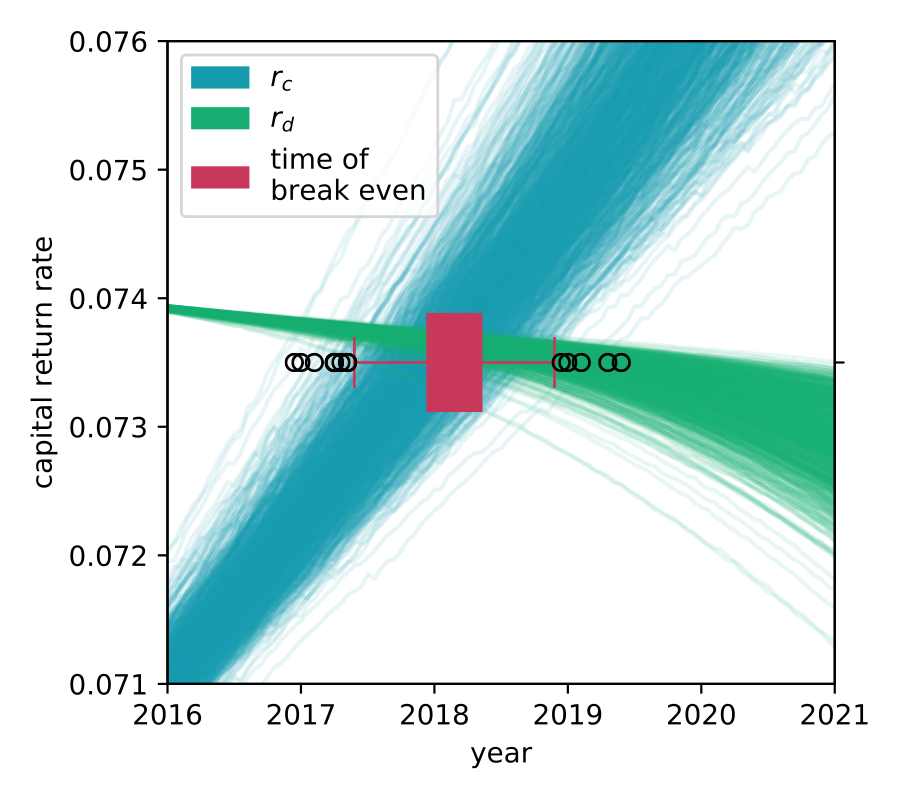
\includegraphics[width = .64 \textwidth]{./figures/break_even.png}
        \caption[Capital return rates in the clean and dirty sector for N=1000 runs]{Capital return rates in the clean and dirty sector for M=1000 runs. Statistical properties of the distribution of intersection times between the return rates in the two sectors are indicated with a box plot.\label{fig:break_even}}
\end{wrapfigure}
%results show social tipping behavior
show a rapid switch in many trajectories from investment primarily in the dirty sector before 2018 to investment primarily in the clean sector after 2018. 

% this social tipping behavior most likely works as follows
This rapid switch is most likely caused by the following mechanism. As shown in \cref{fig:break_even}, the return rate of capital $r_c$ in the clean sector exceeds the return rate of capital $r_d$ in the clean sector in or around the year 2019 -- primarily due to increasing productivity of capital as a result of learning by doing in the sector that increases the knowledge stock $C$. Consequently, households that are `myopic investors' and therefore invest in the sector with the higher capital return rate start to invest their savings in the clean sector. If these households are sufficiently connected to other households that are `herders' or `conformers', the latter may follow their example. Therefore, even though the fraction of myopic investors may be small (their initial frequency is only 1/8th), the fact that their example may be followed by those that decide according to the behavior of their surroundings (whose combined initial frequency is about 1/2) can lead to rapid tipping in the investment behavior of 

the majority of households. This also explains the heterogeneity in final outcomes. As the rapid switch in investment depends on the decision making of households that rely on imitation of the majority of their neighbors, this tipping process is heavily influenced by the micro structure of the model -- particularly the structure of the acquaintance relations between households.

\begin{figure}[H]
	\centering
        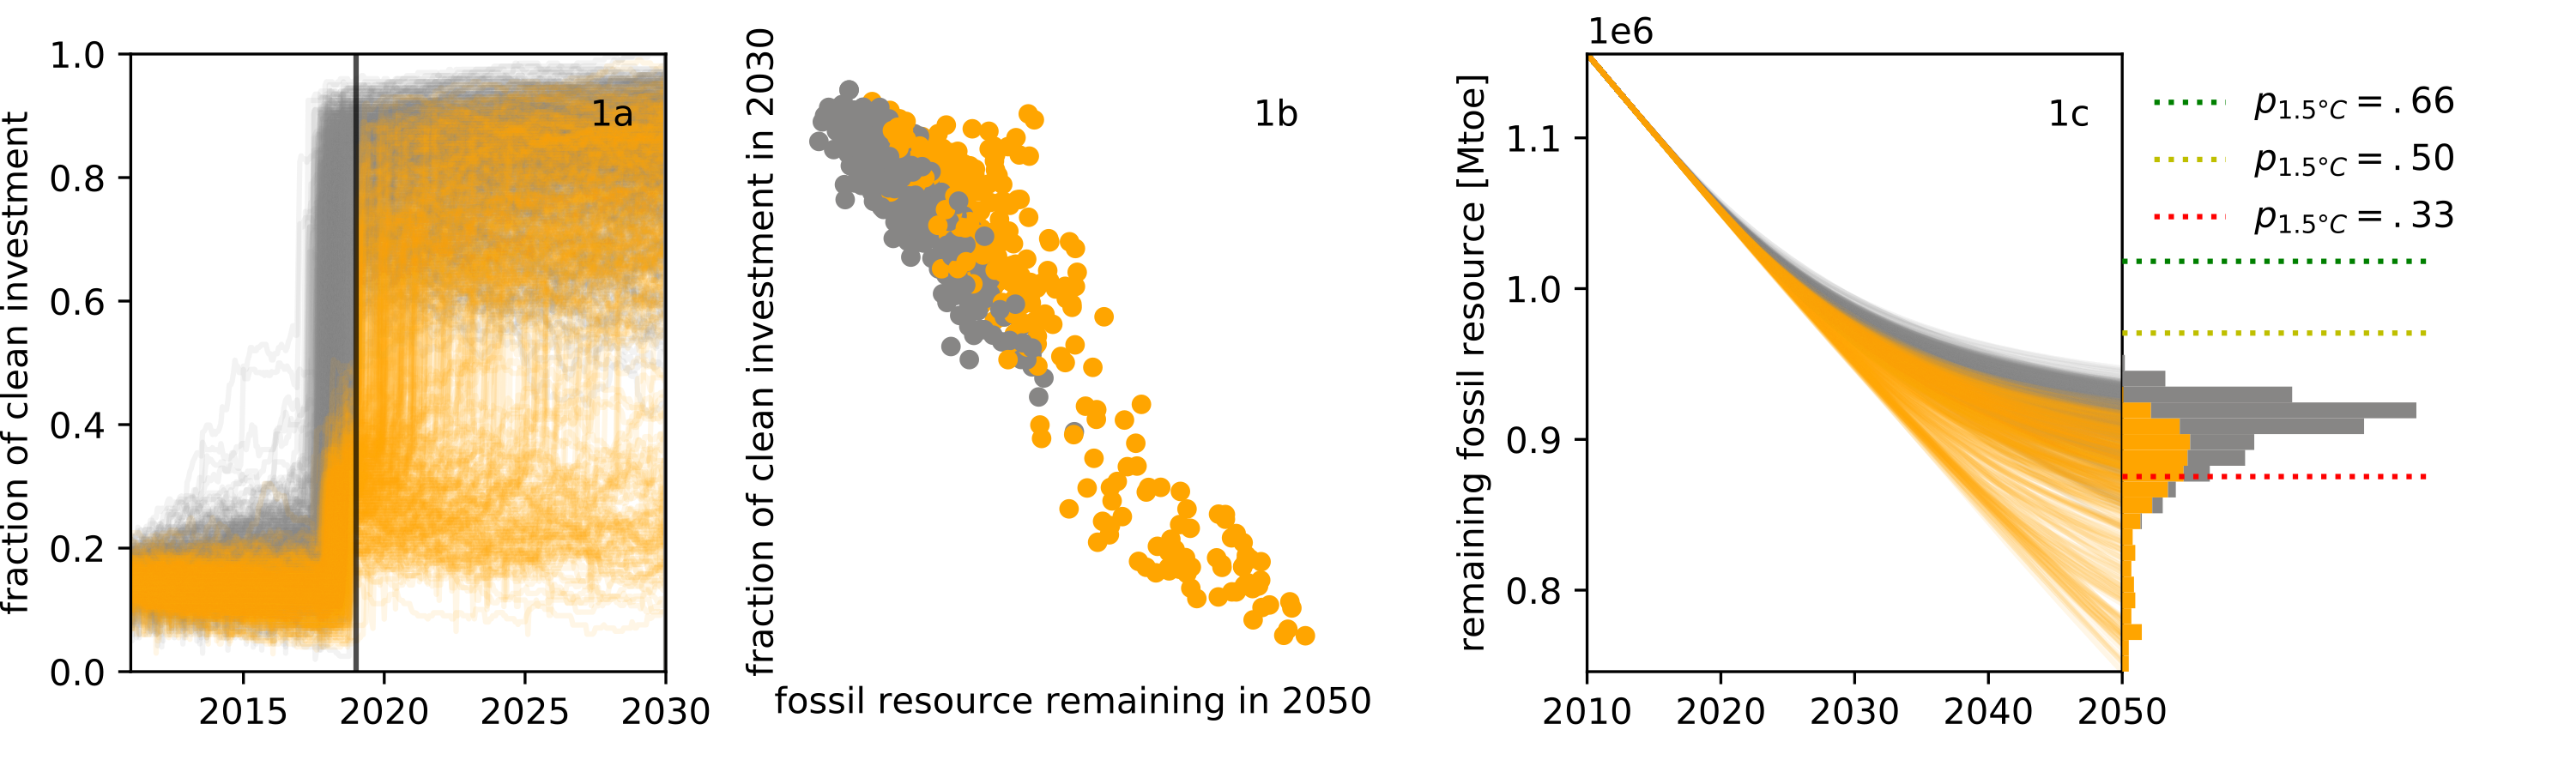
\includegraphics[width = 1.2 \textwidth]{figures/fitted_initials_evaluation05.png}
        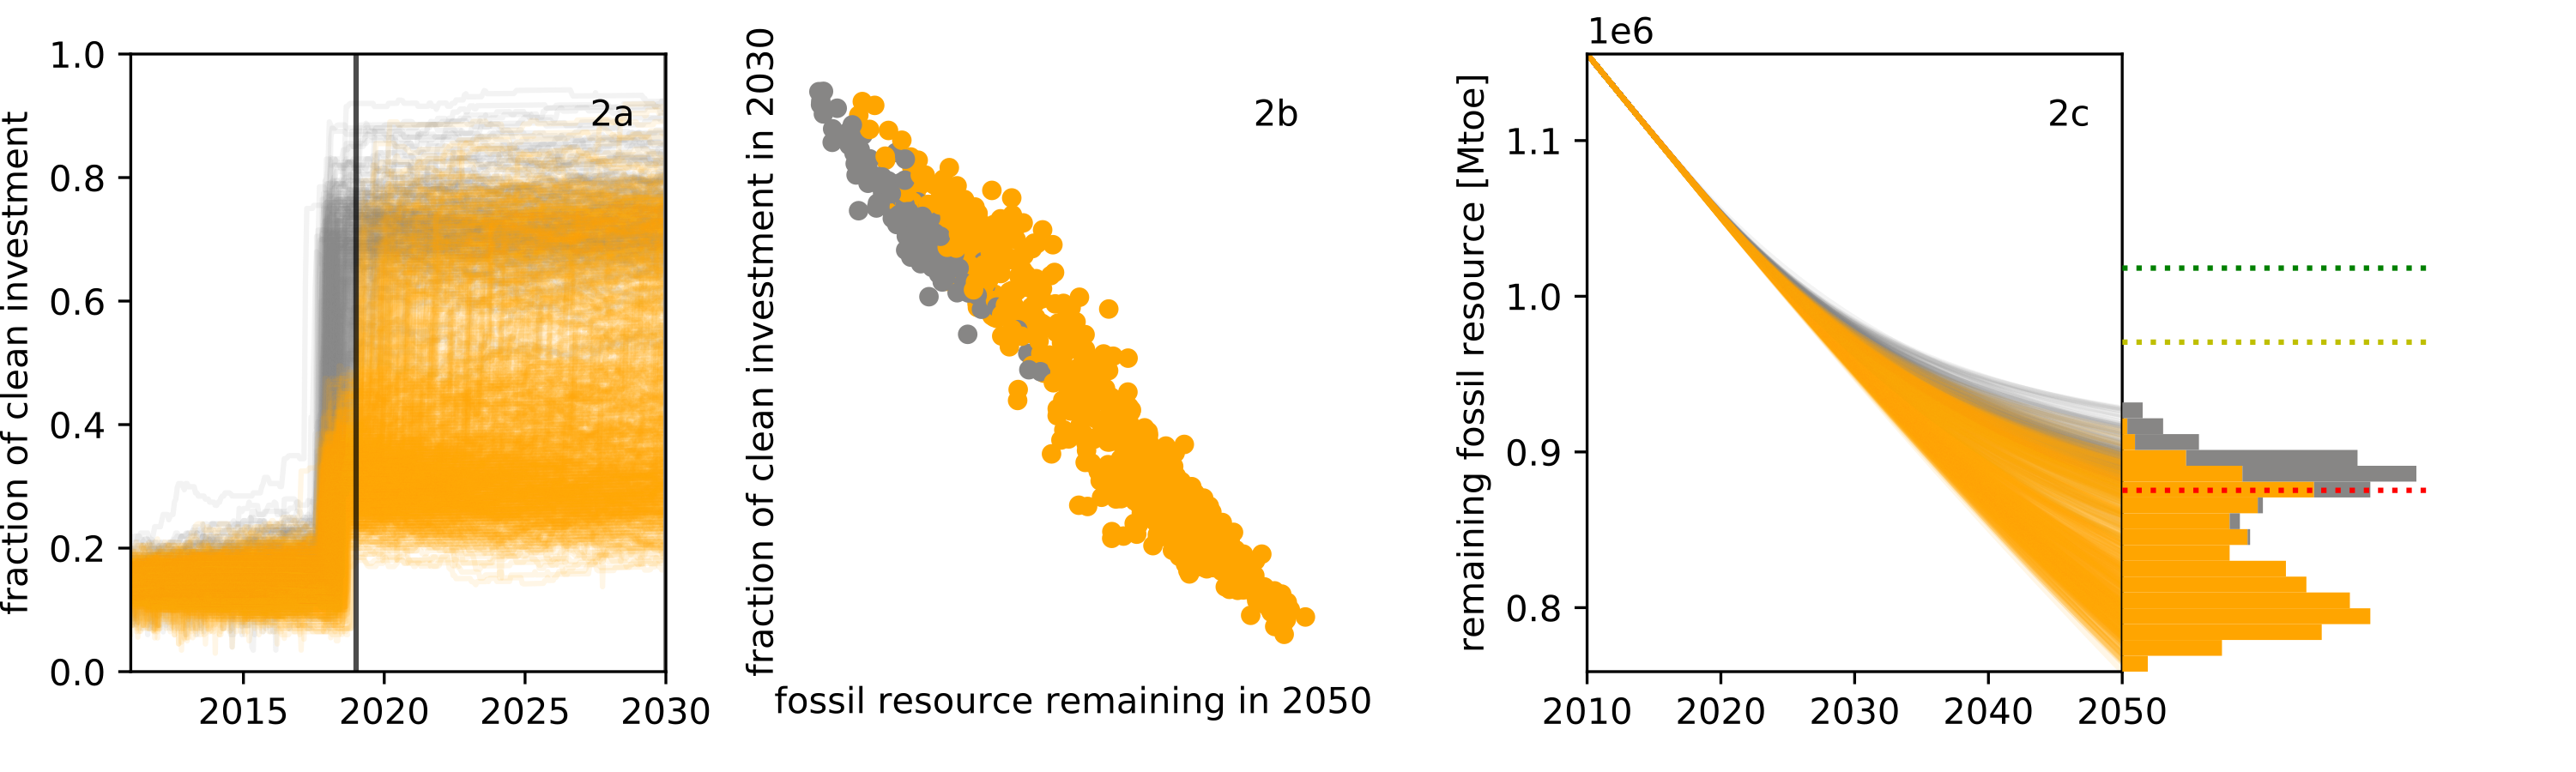
\includegraphics[width = 1.2 \textwidth]{figures/fitted_initials_evaluation07.png}
        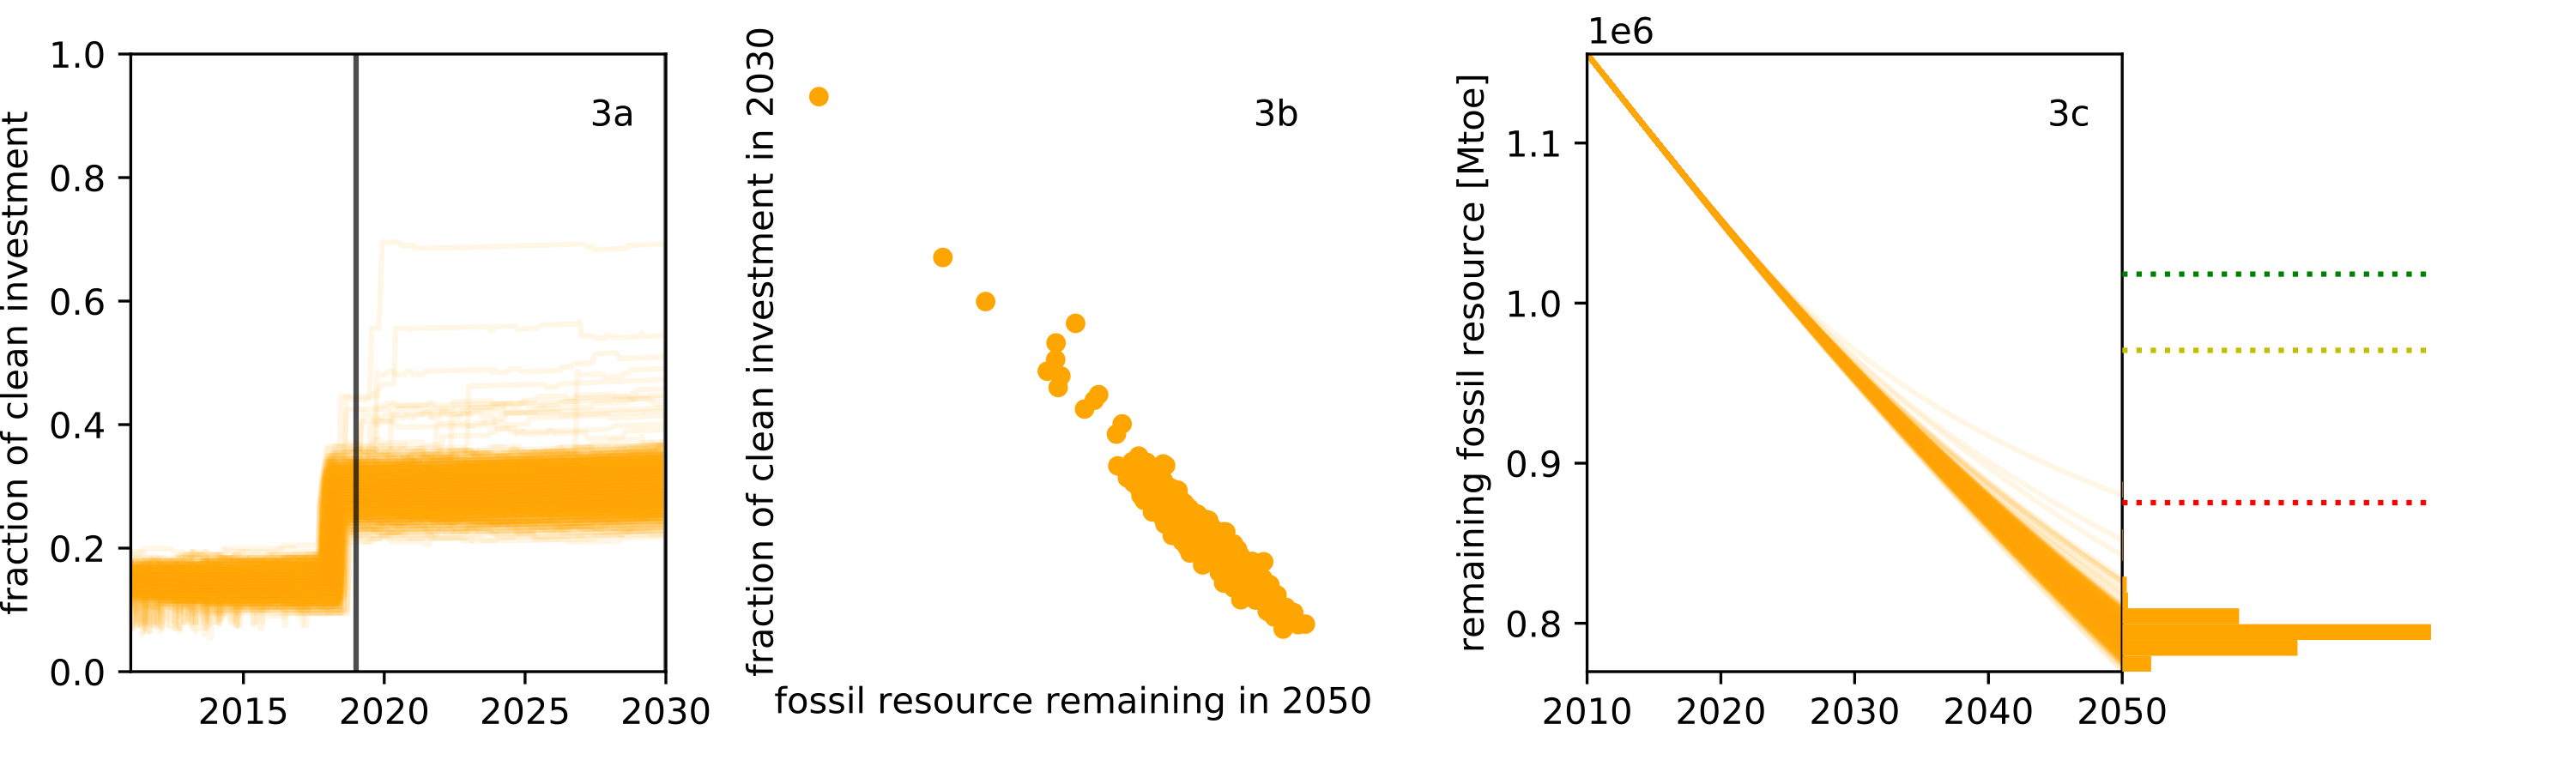
\includegraphics[width = 1.2 \textwidth]{figures/fitted_initials_evaluation09.png}
        \caption[Trajectory of decarbonization transition depending on the network rewiring rate in the social learning process]{\textbf{Decarbonization transition depending on rewiring probability $\gamma$}. Panels 1, 2 and 3 each show ensembles of M=1000 runs with N=100 households, for different rewiring probability 1: $\varphi=0.5$, 2: $\varphi=0.7$ and 3: $\varphi=0.9$. Other parameter values and initial conditions as described in section \ref{sec:parameter_values} and \ref{sec:oppinion_formation_and_decision_making}. Results from runs where the fraction of clean investment exceeds 50\% before 2019 are colored grey. All other results are colored orange. The x and y distributions on the scatter plot in panels b are equal to the distributions of trajectories on the right y axis in panels a and c respectively. The stacked histogram attached to panels c gives the relative frequencies of the bundle of trajectories i.e. the distribution of remaining fossil resource in 2050 over the ensemble of simulations. The dotted lines in these histograms indicate the emission budgets for the $1.5\circ$C target according to IPCC 2013}
        \label{fig:default_alpha_05}
\end{figure}



% tipping in investment only slowly leads to reduction in emissions
Panel 1c shows that this switch of the direction of investment is then later followed by a reduction of the use of the fossil resource. The time lag between the switch of investment and the reduction of resource use is due to the fact that the existing physical capital $K_c$ in the dirty sector is still in productive use and only gradually depreciating over a timescale of approximately $t_{d}^{*}\approx 50$ years as I have shown in section \ref{sec:full_dirty_economy}. It is also clear that not all simulation runs follow this switching behavior and that in a number of runs the majority of investment continues to go to the dirty sector over the entire simulation period or only switches to the clean sector substantially later.

% to set cumulative resource use in perspective, I compare them to emission targets
To set these results into perspective, I have converted the emissions budgets from the IPCC2013 report \citep{stocker2013climate} for the $1.5^{\circ}C$ target roughly into their equivalents in tonnes of oil equivalent in fossil resource use. I show three budgets that are estimated to keep global warming under $1.5^{\circ}$C with different probabilities $p$ and indicated them as dotted lines with the distribution of cumulative resource use on the right edge of panel c. For the conversion, I have used a value of 0.43 metric tonnes CO2 per barrel of crude oil\footnote{https://www.epa.gov/energy/greenhouse-gases-equivalencies-calculator-calculations-and-references} and the definition of one barrel as 0.136 tonnes according to OPEC standards\footnote{https://www.opec.org/library/Annual\%20Statistical\%20Bulletin/interactive/current/FileZ/cfpage.htm}.
In the following, I will call the different budgets
\begin{itemize}
  \item T1 for $p=0.66$ to stay below $1.5^{\circ}$C warming,
  \item T2 for $p=0.5$ to stay below $1.5^{\circ}$C warming and
  \item T3 for $p=0.33$ to stay below $1.5^{\circ}$C warming.
\end{itemize}


% this shows that in the model under the (very optimistic) business as usual scenario, results are bad.
Comparing the results of the model runs in row 1 of \cref{fig:default_alpha_05} with the emission budgets it is apparent that this business as usual scenario of the model exceeds the T2 budget at any rate and even exceeds the T3 budget in many cases. Note that this business as usual scenario can be considered rather optimistic as it assumes technological progress only in clean technologies, and also note that many runs that stay within the T3 budget are colored gray which means that in these cases social tipping happened before 2019. This I would argue is not what happened in the real world and can therefore be considered unrealistic. More to the contrary, if the trigger for a major change in investment from dirty to clean technology will be their relative returns, this would mean that tipping might happen even later in the real world, because e.g. \cite{Farmer2016} predict that this point will only be somewhere between 2025-2030.

% and they get even worse, if the clustering of likeminded households increases.
For the model runs in the first row of \cref{fig:default_alpha_05} it was equally likely for households to break a link and to establish one with a like-minded individual as it was to communicate and possibly update their beliefs if they encountered a differently minded household. 
However, different studies on real world social network data indicate that individuals tend to form clusters of like-minded individuals \citep{girvan2002community, Lerman2010, Law2011, Takhteyev2012}.

Rows 2 and 3 show the dynamics of the model in case the probability for like-minded households to form clusters increases, e.g. for increasing rewiring probability $\varphi$. These results support the previous discussion of the social tipping dynamics depending on the connection between households that rely on economic indicators for their decisions and households that rely on the observation of their peers. If the rewiring probability increases, households that conform with their neighbors cluster together and tend to form groups that self-stabilize in their behavior.

Also, households that use economic indicators to inform their decisions do the same and therefore cannot communicate their decision (in terms of observable behavior) and experience (in therms of generated income) to others. As a result, for $\varphi=0.7$ this leads to a scenario where in some simulations the information can still propagate through the acquaintance network and lead to a social tipping event whereas in other simulations this does not happen, leading in sustained investment in the dirty sector. As a result, the final distribution of cumulative resource use in 2050 is bimodal and runs that exhibit tipping have a chance to stay within the T3 budget while those that do not exhibit tipping exceed it.

If the rewiring probability further increases to $\varphi=0.9$, at the time when investment in the clean sector becomes more profitable, only a fraction of households switch investment to the clean sector. This indicates that propagation of this behavior through the network fails because the network is already too fragmented into unconnected components which is also in line with the segmentation transition that has been shown by \cite{Rogers2013, Wiedermann2015, Klamser2016} and \cite{Min2017} for adaptive voter type models.\\

\textbf{To sum up:}
\begin{itemize}
  \item Decisions of a number of informed individuals in combination with others that rely on the observation of their peers can lead to social tipping in the model given that the tendency of like-minded individuals to cluster together is sufficiently low.
  \item Regardless, in the (rather optimistic) default scenario of the model, emissions are likely to exceed the budget that would keep global warming below $1.5^{\circ}$C with a probability of $p=0.5$.
  \item Especially a tendency of like-minded individuals to cluster together leads to a certain failure to stay within the budget that would keep global warming below $1.5^{\circ}$C with a probability of $p=0.33$ given the model assumptions.
  \item To conclude, in the model world, technological progress and individual choice of households are very unlikely to prevent global warming above $1.5^{\circ}$C.
\end{itemize}




\subsubsection{A Campaign for Clean Investment}
\label{sec:campaign}
The previous section has shown that given the models' assumptions it is unlikely that cumulative fossil resource usage will stay below what is necessary to prevent global warming above $1.5^{\circ}$C. In a default scenario with technological progress in clean technology and individual investment decision making most simulated trajectories exceeded the emissions budget T3 associated with a $p=0.33$ chance of keeping global warming below $1.5^{\circ}$C even for a moderate tendency of like-minded households to cluster together. For higher tendencies of clustering, the modeled economy almost surely exceeds this budget as soon as 2050 without a tendency to slow down fossil resource use.\\

This section will discuss if in the model a social movement in favor of clean investment can drive social tipping to clean investment sufficiently to stay within at least the T2 budget associated with a $p=.5$ chance to keep global warming below $1.5^{\circ}$C.\\

\begin{wrapfigure}[25]{o}{.45 \textwidth}
	\vspace{-.4 cm}
        \hspace{-1.4 cm}
        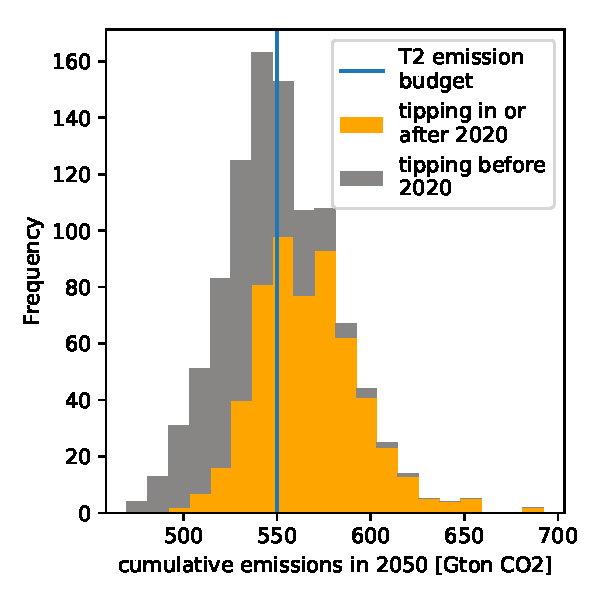
\includegraphics[width = .57 \textwidth]{./figures/emissions_with_campaign.pdf}
        \caption{Stacked histogram for distribution of final cumulative emissions in 2050 for initial campaign sizes between 10\% and 15\% compared to T2 emissions target. \label{fig:campaign_sucess}}
\end{wrapfigure}
Currently, campaigning against the use of fossil fuels takes different forms: \\

Movements like \textit{Extinction Rebellion} and \textit{Ende Gel\"{a}nde} use non-violent means of civil disobedience to stop the economic operation of fossil fuel companies -- especially in the lignite business -- to draw public and media attention to the matter and to influence the public discourse in favor of legislations that limit or prohibit the use of fossil fuels.\\

\textit{Fridays for Future} originated as a student school strike and grew into a coordinated movement that protests to pressure politicians to enact legislations that are in line with the proposals by the IPCC to mitigate global warming.\\

The \textit{Fossil Fuel Divestment Movement} uses classical campaigning tools to advocates the withdrawal of financial capital from firms that are associated with the extraction and burning of fossil fuels. This campaign -- however well intended -- suffers from difficulties. First, even if financial capital is divested from those firms, the physical capital is still there and in operation and potential buyers may be even less inclined to vote for corporate social responsibility. Also previous studies by \cite{Ans2013} suggest that the intended pressuring effects on stock prices that would keep fossil fuel firms from raising new capital necessary for further resource exploration might be small. \cite{SIF2014Report} estimates that only approximately 15 \% of investors invest subject to socially responsible guidelines and that divested holdings are, especially in liquid markets, very likely to quickly find their way to less responsible investors.\\

These campaigns have in common that they want to influence public opinion in favor of mitigating climate change and that they build on a strong mindset of sustainable individual behavior.\\

\begin{figure}[t]
    \centering
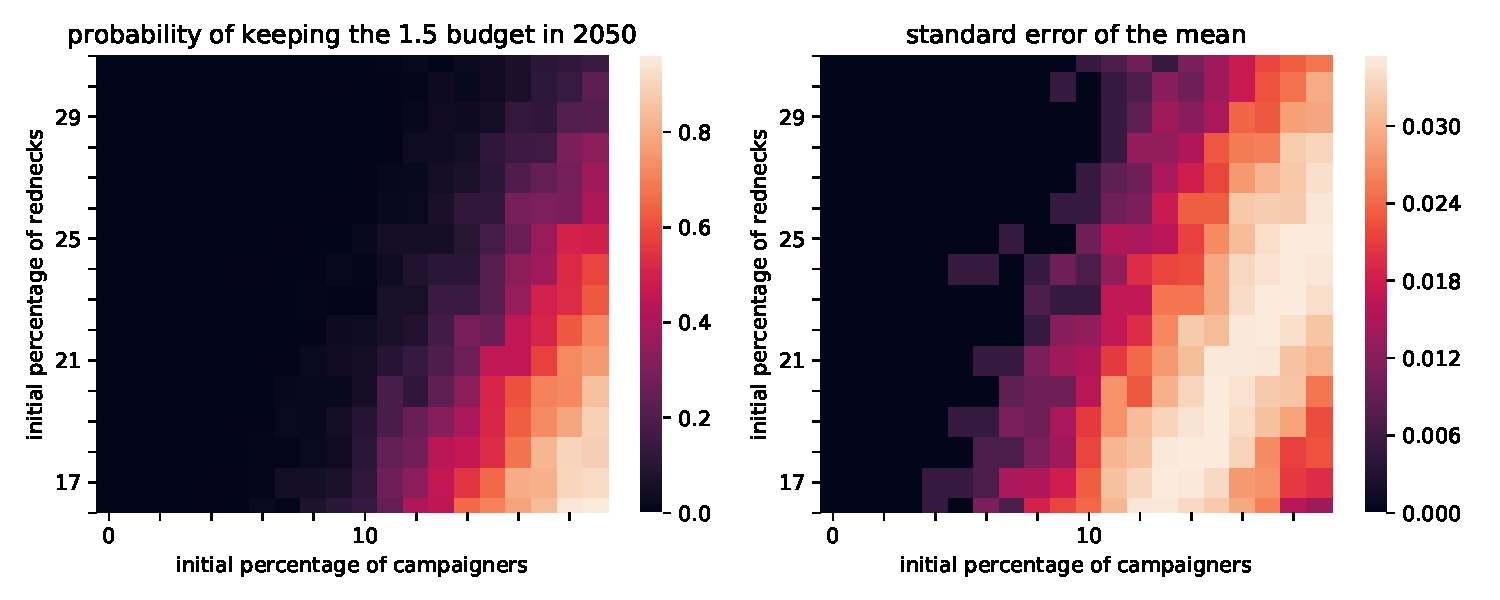
\includegraphics[width = \textwidth]{figures/p_budget15p50_in2050.pdf}
\caption[Probability of staying within the p=0.5, 1,5 degree budget in 2050 depending on the initial size of a campaign in 2010]{Probability of staying within the p=-1.5, 1.5 degree budget in 2050 depending on initial size of campaign in 2010 and initial fraction of rednecks.}
    \label{fig:p15in2050}
\end{figure}

To better understand the possible effects of such campaigning efforts, I implement a social movement/campaign in the model. I measure the success of the campaign as the probability to keep emissions within the T2 budget and analyze the dependence of 
this probability on factors such as the fraction of opposing opinions among the other households, accompanying political measures and the probability of like-minded households to form homogeneous clusters.\\

I implement the campaign in the model in the following way: Members of the campaign will act sustainably e.g. they always invest in the clean sector out of inherent preference (just like the households acting as 'Gutmensch'). In addition, they will not imitate any other reasoning for their behavior. Besides that, members of the campaign interact with other households in the way that is prescribed by the adaptive voter dynamics.\\
\Cref{fig:p15in2050} shows the likelihood of staying within the T2 emissions budget in 2050 depending on the initial size of the campaign in 2010 vs. the initial fraction of opposing opinions ('rednecks'). This shows that for the fraction of opposing opinions of $~15\%$ that I have estimate in section \ref{sec:oppinion_formation_and_decision_making}, emissions can only stay within the T2 budget if the initial campaign size comprise more than $~10\%$ of the population and almost certainly stay within the T2 budget only if the initial size of the campaign exceeds $~15\%$ of the population. Additionally, if the initial fraction of opposing opinions increases linearly, the initial size of the campaign has to increase linearly as well to have the same effect on cumulative emissions.\\

However, a closer look at the results for campaign sizes $n_cp$ between $10\%$ and $15\%$ shows that for many trajectories that stay within the T2 emissions budget tipping happens in or before 2019. To illustrate this, \cref{fig:campaign_sucess} shows the final cumulative emissions in 2050 $E_{2050}$ averaged over $n_{cp}$ between $10\%$ and $15\%$ compared to the T2 emissions budget. The results for trajectories where tipping happens in or before 2019 are given in grey as opposed to the results for trajectories where tipping happens after 2019 that are given in orange. Tipping is classified as the point in time $t_{c90}$ where more than $90\%$ of investment goes into the clean sector e.g. the point in time where investment in the dirty sector is essentially stopped. This shows that in the model the probability to stay within the T2 emissions budget averaged over these campaign sizes of $p(E_{2050}<\mathrm{T2}|10\% \leq n_{cp} \leq 15\%) \approx 0.5$ reduces to $p(E_{2050}<\mathrm{T2}|10\% \leq n_{cp} \leq 15\%, t_{c90}>2019) \approx 0.3$ if one only considers model results where tipping didn't happen before 2019 as I would argue that this is unrealistic.

\begin{figure}[t]
    \centering
    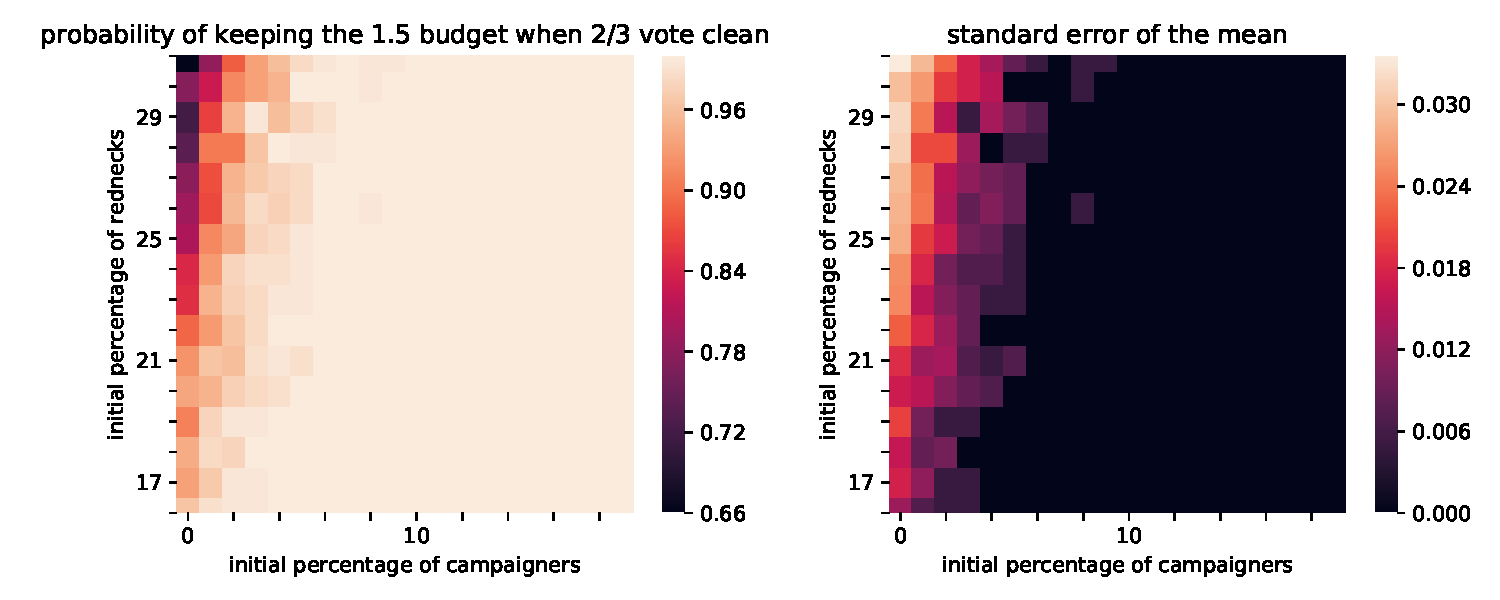
\includegraphics[width = \textwidth]{figures/p_budget15p66_at_campaign_success.pdf}
    \caption{Probability of staying within the p=0.5, 1.5 degree budget when 2/3 of households vote clean depending on the initial size of campaign in 2010 and initial fraction of rednecks.}
    \label{fig:p15sucess}
\end{figure}

The discussion of results presented in \cref{fig:p15in2050,fig:campaign_sucess} indicates that in the model campaigning efforts that aim at norm changes to alter public opinion and individual behavior alone have little prospect of success. However all of the campaigning efforts that I have mentioned above also aim at change in public policy. Therefore, I estimate the likelihood of the success of campaigning efforts that also result in a change in public policy under the most ideal circumstances. Ideal circumstances meaning that as soon as $2/3$rd of the population invest in the clean sector a public policy is implemented that prohibits the further exploration of the fossil resource. This is very optimistic as it neglects vested interests of individuals due to their existing capital in the dirty sector that would be rendered idle by this policy, resulting in a reduction of income of individuals of up to $30\%$.


\Cref{fig:p15sucess} shows the likelihood of cumulative emissions to stay within the T2 budget at the point in time when $2/3$rd of the population decide to stop investing in the dirty sector depending on the initial size of the campaign and the initial fraction of opposing opinions in the population. This shows that as soon as the initial size of the campaign is non-zero, shutting down technologies that rely on fossil fuels as soon as a qualified majority of the population stops investing in them, this would almost surely keep cumulative emissions within the T2 budget. These results show also that even a substantial amount of opposing opinions does not critically endanger the success of the campaigning efforts as even for an initial fraction of $~30\%$ of the population investing in the dirty sector out of their inherent conviction, an initial size of $~1\%$ of the population that takes part in the campaign is sufficient to almost surely lead to social tipping in favor of the clean sector before the T2 budget is exceeded.

This shows that in the model campaigning in combination with strict public policy at the soonest point in time when it would possibly be politically viable is in principle capable of preventing global warming above $1.5^{\circ}$C.
However, political realities show that public policy is rarely as strict as banning an entire sector at once and that it usually comes with substantial interim periods to reduce potential fallout to a minimum. Also, bans are usually the ultima ratio and policy makers usually prefer methods that rely on voluntary self-commitment and technological change as long as possible.

\begin{figure}[t]
    \centering
    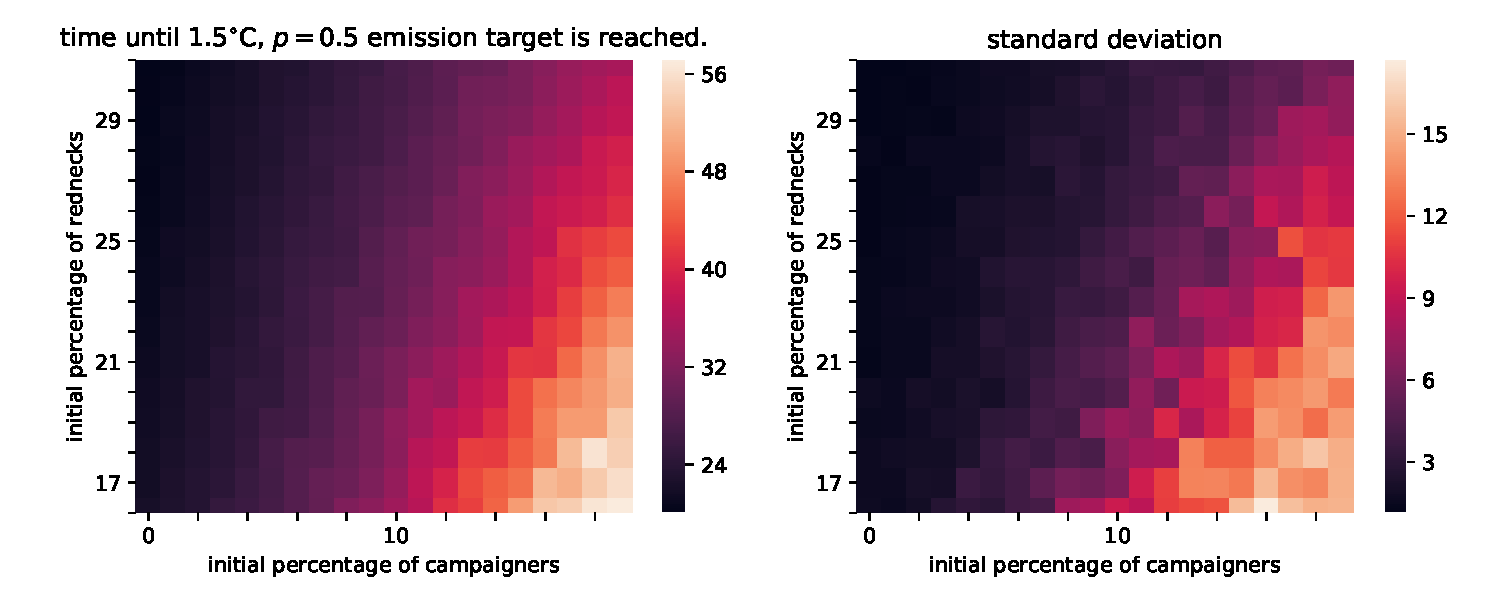
\includegraphics[width = \textwidth]{figures/time_until_emissions_target.pdf}
    \caption{Time until the p=0.5, 1.5 degree budget is used up depending on the initial size of campaign in 2010 and initial fraction of rednecks.}
    \label{fig:time_until_budget_reached}
\end{figure}

Therefore, I want to analyze how long campaigning efforts could possibly elongate the window of opportunity for softer policy measures before dirty technologies would eventually have to be banned to stay within the T2 budget. \Cref{fig:time_until_budget_reached} shows the time until the T2 budget is reached depending on the initial size of the campaign and the initial fraction of opposing opinions in the population. 
\begin{wrapfigure}[26]{o}{.45 \textwidth}
	\vspace{-.4 cm}
        \hspace{-1.4 cm}
        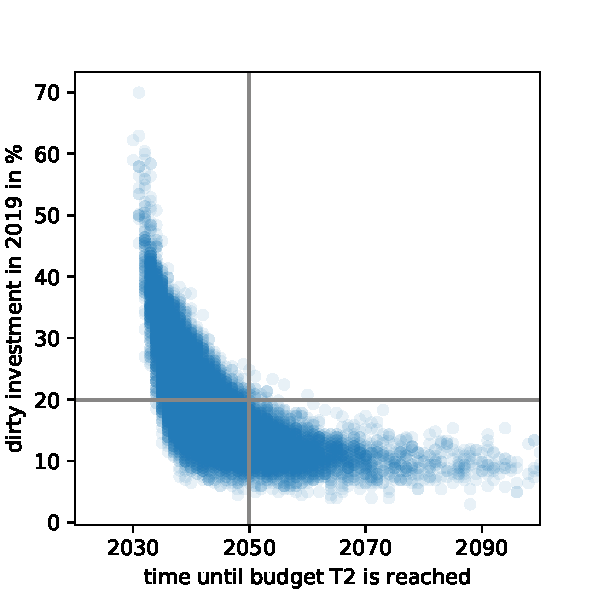
\includegraphics[width = .57 \textwidth]{./figures/dirty_investment_consequences.pdf}
        \caption{Scatter plot of percentage of investment in the dirty sector vs. the time until the T2 emissions budget is reached for an initial fraction of opposing opinions of 16\% to $20\%$ and an initial fraction of campaigners of $10\%$ to $15\%$. \label{fig:dirty_investment_consequences}}
\end{wrapfigure}
These results show that for an initial fraction of opposing opinions of $~15\%$ as projected in section \ref{sec:oppinion_formation_and_decision_making}, campaigning can increase the time window substantially from until 2023 with no initial campaign in 2010 to up to until 2066 if the initial campaign size in 2010 were $~15\%$ of the population. 
However, the elongation of the time window for clean technologies to establish on a voluntary basis would come from essentially halting almost all investment in dirty technology as soon as 2019 to only use the existing capital stock in the dirty sector until it depreciates. \Cref{fig:dirty_investment_consequences} shows the fraction of dirty investment in 2019 vs. the time until the T2 emissions budget is reached. 
Here, it is apparent that less then $20\%$ of investment in the dirty sector in 2019 is a necessary, yet not sufficient condition for the extension of the time frame until the T2 budget is exceeded beyond 2050. In simple words this means that every car that is sold today reduces the probability that this same car (or any other brand new car for that matter) could be used until the end of its life cycle should one seriously intend to keep emissions within the T2 budget.

Finally, I want to examine how the tendency of like-minded households to form clusters influences the probability of success of a campaign that advocates clean investment. Therefore, \cref{fig:campaign_phi} shows the mean and standard deviation of cumulative emissions at the success of the campaign e.g. when 2/3rd of households invest in the clean sector for varying initial size of the campaign and the rewiring probability $\varphi$. Here, a rewiring probability of $\varphi<0.6$ e.g. a low to medium tendency of like-minded households to cluster together has little to now effect on the prospects of campaigning efforts. However, if the rewiring probability increases, the model exhibits a transition to a state where campaigning efforts become futile for a campaign that starts with less than $15\%$ of participation in 2010. This is not surprising, as e.g. \cite{Rogers2013, Wiedermann2015} and \cite{Klamser2016} have shown before that for a rewiring probability $\varphi$ above a critical value, adaptive voter type network dynamics undergo a segmentation transition where an initially fully connected graph decomposes into smaller unconnected sub graphs of nodes that share the same state/opinion. This also happens in this model -- somewhat attenuated by the exploration behavior of households that acts as noise to the adaptive voter dynamics and therefore facilitates some connection between otherwise disconnected homogeneous clusters of households.\\

In this light, the fact that an initial campaign size of $20\%$ can still lead to social tipping e.g. 2/3rd of households investing in the clean sector can be explained by the models initial conditions. Initially, the acquaintance graph between households is fully connected and household opinions are set regardless of the network topology. This fully connected network needs some time to decompose into disconnected clusters which in return means that there is a limited time frame in which social tipping can happen. This however also means that this effect is somewhat artificial since -- given the assumption of homphilic association among households holds -- real networks would exhibit some correlation of clustering and individual traits already in their initial conditions.\\

\begin{figure}[t]
    \centering
    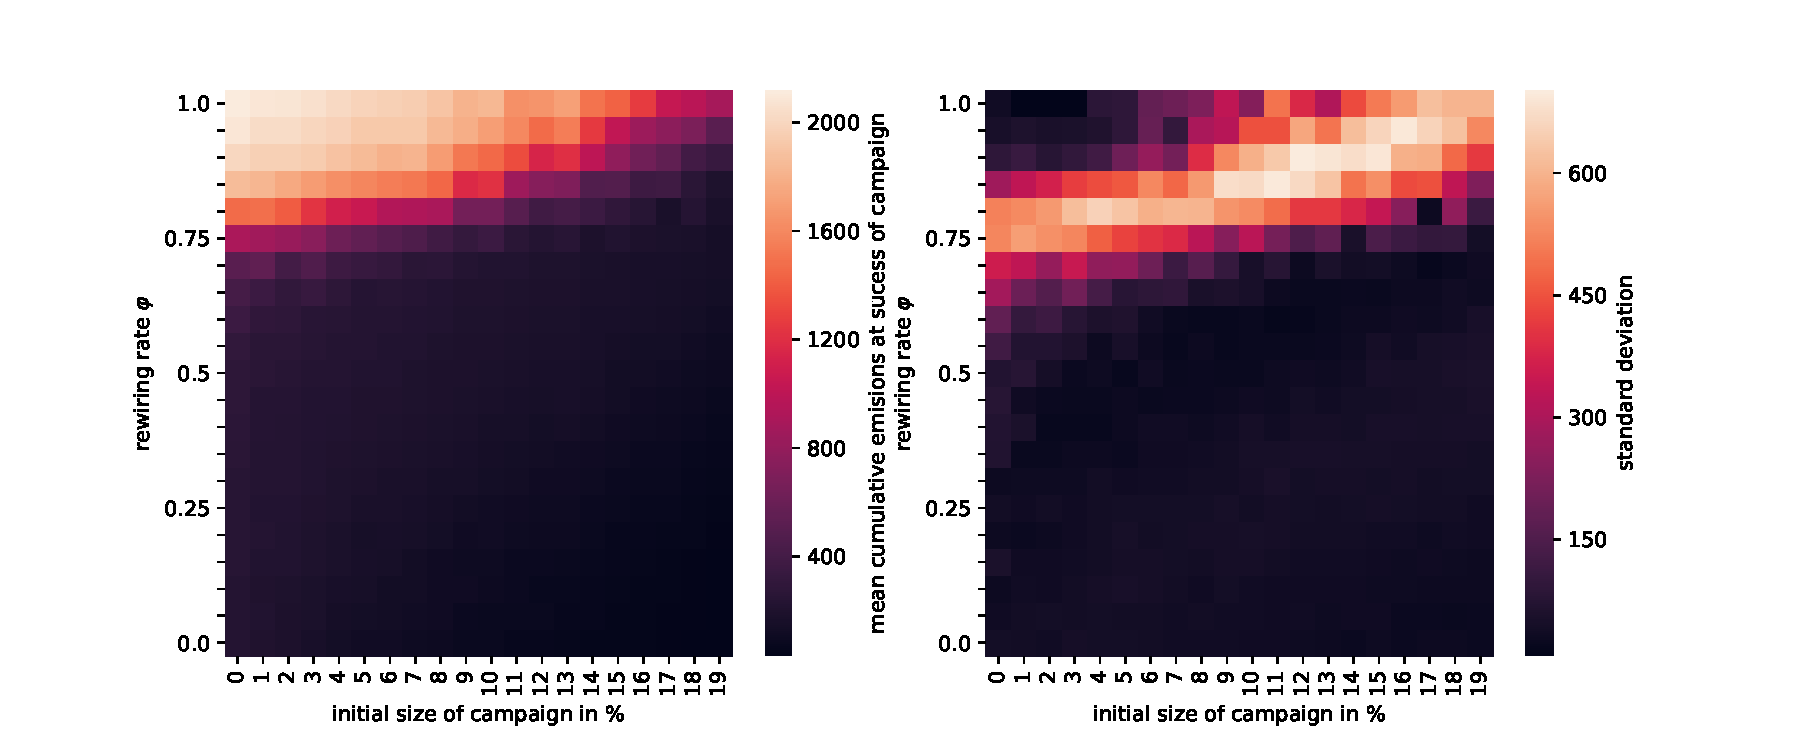
\includegraphics[width = \textwidth]{figures/campaign_vs_phi.pdf}
    \caption{Mean and standard deviation of cumulative emissions at the success of the campaign depending on the initial size of the campaign and the rewiring probability $\varphi$ that is a parameter for the tendency of like-minded households to cluster together. }
    \label{fig:campaign_phi}
\end{figure}

To sum up, I showed that in this model:
\begin{itemize}
  \item Campaigning to stop investment in dirty technologies alone has little to no chance to prevent global warming above $1.5^{\circ}$C if climate change mitigation only happens through technological progress and individual decision making.
  \item Complementing a campaign, a strict public policy that prevents the use of fossil resources has the potential to limit global warming below $1.5^{\circ}$C if it is implemented as soon as it is politically opportune e.g. as soon as a qualified majority of 2/3rd of households invest in the clean sector.
  \item Even though campaigning cannot prevent global warming above $1.5^{\circ}$C, it can substantially extend the window of opportunity to come up with less strict measures to halt the use of fossil fuels given that it successfully halts investment in the dirty sector.
  \item In the model, the dependence of the prospects of success of campaigning efforts on the dendency of like-minded individuals to cluster together is highly nonlinear due to a segmentation transition in the underlying adaptive voter dynamic.
\end{itemize}

\section{Discussion and Conclusion}
\label{sec:heuristics_conclusion}

% what did i do (maybe also shortly reiterate why)
In the previous chapter, I developed, calibrated and analyzed a model that combines social learning and individual, bounded rational decision making with elements of neoclassical economics to model sustainability transitions away from fossil fuels.
In the model, heterogeneous households are owners of capital and labor that they use to generate income. The households save a fixed amount of their income and decide between a `clean' and a `dirty' sector in which they can invest their savings. The `dirty' sectors uses a fossil resource for production whereas the `clean' sector uses a clean technology that is still under development. In this stylized production economy, capital rents and wages in the two sectors as well as fossil resource use in the dirty sector form subject to aggregated supply and demand of labor and capital.
In this context, the model describes the interplay of social dynamics and individual processing of information from different sources that lead to collective behavior of individuals. This collective behavior in return shapes the environment in which the modelled individual live.
In contrast to many other social-ecological models, this model differentiates between judgement and action of individuals. In most social-ecological models that emulate individual opinion formation, behavior, opinion and action are equivalent and spread via imitation of successful behavior. In contrast, in this model individuals learn heuristics that they use to judge which action would be best given the circumstances.

% how did i do it
I used adaptive network dynamics for social learning, ordinary differential equations with algebraic constraints to model economic dynamics economic dynamics and fast and frugal heuristics to describe individual decision making individual decision making.
I solved the algebraic constraints of the model analytically and I roughly estimated parameters from data where possible. I complemented this with the analysis of different limiting scenarios to estimate the parameter dependence of timescales for different processes in the model and I conducted numeric experiments to analyze the models default behavior.
I implemented a social movement in the model in which members of the movement only ever invested in the clean sector and did -- unlike the other households -- not change their judgement heuristic subject to the social learning process. Subsequently, I conducted different numeric simulation experiments to analyze the prospects of success of such a campaign in the given model subject to different parameters and potential accompanying public policy measures.

% what are shortcomings of the model
The model that is developed and analyzed in this chapter is conceptual and as such it is stylized and oversimplified in many respects.
For instance it does not consider any climate damages and does not differentiate between different fossil resources and sources of emissions. Its economic model is simplistic as in reality many kinds of physical capital are not explicitly connected to a specific sector and can be reallocated. Also, investment decisions are rarely as simple as deciding between two sectors to invest in. Rather, making investment decisions has increasingly become a science of its own.\\
Considering these shortcomings of the model, its results should by no means be understood as actual predictions. However, it still pictures general trends and allows insights into effects that emerge from interactions of different processes that are -- at least in this combination -- usually not considered together.

% what were the results
The results of the numeric simulations that I conducted indicate that given the underlying assumptions of the model, campaigning efforts that advocate investment in carbon free technologies alone have only a very limited chance of mitigating global warming above $1.5^{\circ}$C as in realistic scenarios they are unable to limit cumulative emissions to the T2 budget that limits global warming below $1.5^{\circ}$C with a probability of $p=0.5$ in the IPCCs projections.
Measuring the cumulative emissions at the point in time when two thirds of households started to invest in the clean sector however suggest that if at this point a public policy could be implemented to ban the use of fossil fuels, cumulative emissions could be kept within the T2 budget almost certainly. 
Unsurprisingly, the evaluation of these experiments also shows that campaigning that leads to reduced investment in fossil fuel dependent technology in favor of increased investment in clean technologies increases the window of opportunity that could be used for mitigation measures that are softer than a ban before the T2 budged is exceeded.

% what is the significance of the results in a broader context
The results give hope that it might be possible to still mitigate global warming above $1.5^{\circ}$C and strongly suggest that to this end a number of different, complementary measures will be needed. They suggest that a timely phase out of investment in technologies that rely on fossil fuels is a crucial step to mitigate global warming. The suggest that for public opinion to swing in favor of clean technologies, these technologies have to be viable and competitive also in the short term. This can and already has been facilitated with appropriate subsidies, market design and taxation. The results also suggest that at some point certain dirty technologies will have to be shut down and that capital associated with these technologies will have to be written of. This is already happening -- in Germany at least -- but might have to happen sooner and on a much larger scale to actually have the desired effects on cumulative emissions. Finally, the results strongly suggest that campaigning can help to influence individual decisions and public opinion to an extent that makes the aforementioned measures politically viable and their consequences less severe. But the results also indicate that strong clustering of like-minded individuals such as in political polarization and the formation of filter bubbles that allow completely disconnected and fragmented discourses to coexist can render such campaigning efforts entirely futile.

% what else can be done.
In the analysis of the model, I considered a combination of campaigning and public policy measures that are aimed to ban the use of fossil fuels. However, a model along these lines would also allow to analyse the effects of a number of other policy measures.
Obvious candidates would be taxation for dirty and subsidies for clean technologies similar to \cite{Geier2019}. A not so extensively yet interesting policy measure would be marketing strategies such as nudging and priming that aim to influence an individuals internal evaluation of different options and often time explicitly anticipate heuristic decision making. Priming for instance aims to activate certain concepts in individuals' minds to make them consider aspects related to this concept over other unrelated aspects in their decisions. In this framework such measures can be implemented by temporarily altering individuals' cue orders after exposure to marketing efforts.

% what can be done better
To make this model more realistic, one could consider a number of improvements and extensions. With regards to the economic dynamics, one can consider technological progress also in the dirty sector as well as a possible third sector that does not depend on either of the two technologies. For instance production of energy could be divided into fossil and renewable energy production and production of final goods can happen in a separated sector as e.g. in \cite{Heitzig2015a}. In individual decision making natural extensions would be the consideration of more possible cues and the full spectrum of the resulting cue orders as well as other modi of decision making such as alternative heuristics that fit the decision environment (such as tallying) or to consider more sophisticated decision strategies (such as utility maximization in combination with Bayesian updating) to take account of the fact that especially bigger investors certainly use more complex and elaborated decision making tools. With respect to social learning one can consider the fact that in this model individual parameters are homogeneous between agents. However in real world systems the preference for homphilic rewiring is likely to be heterogeneous between individuals. For instance empirical studies on Optimal Distinctiveness Theory \cite{hornsey1999subgroup, leonardelli2010optimal} find that the preference for relationships with individuals with similar traits is heterogeneous within the groups under study.
Also, one can consider that individuals may not only learn how do decide where to invest but maybe also how much. With that regard, the subsequent chapter will elaborate on the interesting possible effects of individuals that use social learning to set their savings rate in a one sector production economy.

        \chapter{Emergent inequality in a simple behavioral macroeconomic model}
\label{chapter:savings}

This chapter is based on research that I have designed, prepared and supervised. Results are part of \citep[P4]{Asano2019}. In this chapter I analyze the role of agent heterogeneity in a simple economic investment model where agents use a social learning heuristic to set their individual savings rates. To this end, I use a simplification of the heterogeneous agent investment model introduced in the previous chapter. This model is equivalent to an extension of the standard Ramsey-Cass-Koopmans (RCK) model to heterogeneous bounded rational households. Unexpectedly, this extended model is capable of producing endogenous oscillations in economic output resembling a business cycle. This is noteworthy as standard economic models usually depict business cycles not as endogenous dynamics but as the result of repeated exogenous shocks. In section \ref{sec:savings_introduction}, I motivate the use of heterogeneous bounded rational agents in economic growth and savings models to study emergent endogenous dynamics. Subsequently, I discuss the standard RCK model in section \ref{sec:savings_standard_rck} which is one of the foundational economic growth models. Based on this model, I give the specifications of the simplified agent-based heterogeneous household savings model in section \ref{sec:savings_model}. I present results of numerical simulations of the adapted model in section \ref{sec:savings_results} and discuss two different dynamical regimes of the model as well as the transition between them before concluding.

\section{Introduction}
\label{sec:savings_introduction}
Economic growth and inequality are important problems in economics \citep{Acemoglu2009, piketty2015capital}. Standard macroeconomic models are based on the assumption of a single representative rational utility maximizing agent and assume that the dynamics of business cycles are driven by exogenous shocks. However, empirical evidence from behavioral economics indicates that real households are heterogeneous and make substantial deviations from rationality.   This has led to new directions of research, including the incorporation of heterogeneous or bounded rational agents into macroeconomic models. This is typically done by allowing the agents to differ in terms of factors such as education while preserving the assumption of rationality \citep{ hank_reviewLeahy2018, hank_branch2009new, hank_zhao2018many}, or alternatively allowing for bounded rationality but maintaining utility maximization \citep{hank_gabaix2016behavioral}.  Realism is injected through imposing frictions, such as sticky wages.  These models require shocks to generate economic dynamics.

However, it has long been known that endogenous dynamics are possible in economic models~\citep{day1983emergence,BOLDRIN198626, Scheinkman, boldrin1992equilibrium, boldrin1992sources,blume1992evolution}, and more recently Beaudry \textit{et al.}\ have shown how limit cycles can emerge in a standard framework where agents are perfect utility maximizers \citep{beaudry2015reviving, beaudry2016putting}.  An alternative approach bases household decision making on simple heuristics rather than rationality \citep{DeGrauwe2011,DeGrauwe2010the}.  This leads to ``waves'' of optimism and pessimism, generating irregular business cycles and giving fat-tailed distributions for economic outcomes such as GDP. This chapter further develops this line of research by demonstrating how a very simple heterogeneous behavioral macroeconomic model leads to an endogenous business cycle that is not driven by externally imposed shocks. The purpose here is not to make a fully realistic model, but rather to demonstrate that rich emergent behavior can occur even under very simple assumptions.

This is done by extending the RCK model, which is one of the foundational models of economic growth theory. In this model a representative agent rationally chooses a savings rate in order to maximize discounted consumption.  However, there is ample evidence that households do not act as intertemporal optimizing agents and often respond myopically~\citep{Benartzi1995,Loewenstein2000,Choi2016}.  Evidence from lab experiments suggests that individuals perform poorly in finding optimal consumption paths. For instance, subjects deviated from optimal consumption choices by roughly 30 percent on average, increasing to roughly 50 percent when subjects were shown the average consumption level in the previous period  \citep{carbone2014lifecycle}.  Learning from past generations' consumption paths is somewhat more successful, but the errors are still substantial \citep{ballinger2003precautionary,brown2009learning}.  

Here, I take the opposite approach and assume a strong form of bounded rationality.  In this model households are embedded in a social network and make their savings decisions by simply copying their most successful neighbor. They do this episodically and myopically: From time to time they check all their neighbors and adopt the savings rate of the neighbor with the highest consumption.   

Although I do not claim that this behavior is fully realistic, there is empirical justification for considering a simple rule of this type.  The agents can be viewed as short-sighted, profligate ``conspicuous consumers'', and the tendency of households to copy one another has been well-documented since the time of Thorstein Veblen \citep{veblen1899}.  Imitate-the-best is one of the decision-making heuristics often applied in settings of high uncertainty and variability~\citep{Gigerenzer2011} and is observed in economic experiments~\citep{Traulsen2010}.  Savings behavior is highly dependent on social interaction with peers~\citep{Lu2011,Zhang2018,Kaustia2012, cascades} and comparing consumption levels incorporates the visibility bias and selection neglect observed in savings rate decisions~\citep{enke2015you}.  This implementation by copying based on consumption alone is partly motivated by the fact that a neighbor's consumption is more visible than their capital.    This makes it particularly surprising that in some circumstances their average behavior can be close to optimal.

I find that a key parameter governing economic behavior is the average time interval $\tau$ at which households update their savings rate, which I call the \textit{social interaction time}.  When $\tau$ is small, meaning the households update frequently, the savings rate is low, and the performance of the economy is suboptimal in terms of aggregate consumption. When $\tau$ is sufficiently large, in contrast, the economy-wide aggregate savings rate, which equals the income-weighted average household savings rate, becomes close to the optimal rate.  For small $\tau$ the population of households remains homogeneous, but as $\tau$ increases there is a sharp phase transition at a critical value $\tau_{c}$ where the population becomes strongly bimodal, dividing into rich households with high savings rates and poor households with low savings rates.  Correspondingly, for low values of $\tau$ the GDP and other economic indicators are constant with only small fluctuations, whereas above the critical transition there is an endogenous aperiodic oscillation, resembling a business cycle, in which the aggregate savings rate fluctuates, the population of households alternately becomes richer or poorer, and economic output varies substantially over time.  

This model shows that the use of heterogeneous agents following explicit behavioral rules can produce aggregate behavior that is qualitatively different from that of rational agents. This model is only qualitative, but its results suggest that an approach that explicitly incorporates empirical behavioral knowledge into household decision making may naturally lead to an explanation of business cycles in terms of endogenous dynamics. 
\section{The Standard Ramsey-Cass-Koopmans model}
\label{sec:savings_standard_rck}

The following formulation of the standard Ramsey-Cass-Koopmans (RCK) model is based on refs. \cite[p. 287--317]{Acemoglu2009}, \cite[p. 85--135]{Barro2004}  and \cite[p. 38--90]{Blanchard1989} and uses continuous time, as in the original study \citep{Ramsey1928}.

Like many economic models, the standard RCK model studies the behavior of only one, infinitely lived, ``representative'' household with a strictly increasing and strictly concave utility function $u(c)$ depending only on consumption $c$. This household supplies labor $L$ and capital $K$ to a single representative firm that produces a single good $Y$ assuming a Cobb--Douglas production function
\begin{equation}
  Y \! =\! K^\alpha L^{1-\alpha}\label{eq:CD-Production}
\end{equation} 
with capital and labor elasticities $\alpha, 1 \!- \! \alpha \in (0,1)$.
In contrast to the original formulation of the model, I abstract from modeling labor growth as this is not relevant to the dynamics that I am interested in.
Per-capita production, $y \! =\! Y/L$, is thus a function of per-capita capital, $k \! =\! K/L$, only such that $y \! =\! k^\alpha$.

The RCK model assumes fully competitive factor markets. Consequently, as already discussed in section \ref{sec:model_description}, the two factors are compensated according to their marginal products, resulting in wages and capital rents as follows:
\begin{align}
  &w = \frac{\partial Y}{\partial L} = (1 - \alpha) y, \label{eq:wages}\\
  &r = \frac{\partial Y}{\partial K} = \alpha y /k. \label{eq:capital_rents}
\end{align}
This also means that the produced good is fully redistributed to the representative household leaving the representative firm with no profits.
The main model parameters of interest are the savings rate $s \le 1$ (which is allowed to be negative to reflect borrowing) 
and capital depreciation rate $\delta > 0$. These parameters govern aggregate and per-capita capital growth as follows, 
\begin{equation}
        \dot{K} = s(rK + wL) - \delta K,
        \quad \dot k = \bar{r}k + w - c,
\label{eq:kdot}
\end{equation}
where $\bar{r}=r-\delta$ is the real return rate and $c=(1-s)(rk+w)$ is per-capita consumption.
The household is assumed to maximize its discounted aggregate utility
\begin{equation}
        \int_0^{\infty} \! \mathrm{d}t \, e^{-\rho t} u(c(t)), 
        \label{eq:int1}
\end{equation}
by choosing an optimal path $s(t)$ for the savings rate, where $\rho>0$ is its discount rate.
To avoid that the representative household borrows money to shift its future consumption to the present and then continuously rolls over the existing debt into the future, one imposes a so called `No-Ponzi-Game' (NPG) condition \citep[p. 292]{Acemoglu2009}:
\begin{equation}
  \lim_{t \rightarrow \infty} k(t) e^{-\int_{0}^{t}d\tau \bar{r}(\tau)} \geq 0
  \label{eq:NPG}
\end{equation}
This equation ensures that households do not borrow more than they eventually receive and is equivalent to the future capital having a positive present value.
Thus, the task of the household is to find a path $(k(t),c(t))$ that optimizes equation \eqref{eq:int1} and satisfies equations \eqref{eq:kdot}  and \eqref{eq:NPG}.

\subsection{The RCK model's steady state}
For the instantaneous utility, one assumes a constant relative risk aversion (CRRA) function parameterized by
\begin{equation}
  u(c) = (c^{1-\theta} -1)/(1-\theta)~\mathrm{where}~\theta \geq0~\mathrm{and}~ \theta \neq 1.
  \label{eq:carra}
\end{equation}
Solving the intertemporal optimization problem posed by eq.~\eqref{eq:int1} subject to the constraints given by eqs.~\eqref{eq:kdot} and \eqref{eq:NPG} with the utility function \eqref{eq:carra} results in the Ramsey-Keynes equation
\begin{equation}
  \frac{\dot{c}}{c} = \frac{\bar{r} - \rho}{\theta}
  \label{eq:ramsey_keynes}
\end{equation}
that gives the relative growth rate of consumption depending on the real return rate on capital $\bar{r}$, the households discounting rate $\rho$ and the elasticity of its marginal utility $\theta$.\\

In particular, this system has two steady states with $\dot c\!=\!0$, a trivial one in which $c\!=\!k\!=\!0$ and another in which 
the real return rate equals the discount rate, $\bar r \!=\! \rho$, corresponding to a modified `golden rule' \citep[p. 300]{Acemoglu2009}. In this non-trivial steady state capital, consumption and savings rate are given by
\begin{equation}
	k^\ast = \left(\frac{\alpha}{\rho + \delta}\right)^{\frac{1}{1-\alpha}}, 
 	\quad c^\ast = {k^\ast}^{\alpha} -  \delta k^\ast,
 	\quad s^\ast_\mathrm{RCK} = \frac{\alpha \delta}{\rho + \delta}. \label{eq:rck_steady_state}
\end{equation}
For the limit case $\rho\to 0$, this reproduces the Solow model's golden rule \citep[p. 35]{Barro2004}, 
\begin{equation}
  s^\ast_\mathrm{RCK} \! =s_\mathrm{gold} \!=\! \alpha.
  \label{eq:golden_rule}
\end{equation}
This is called the golden rule because $s = \alpha$ leads to the largest possible sustainable consumption,
\begin{equation}
        c^\ast \! =\!(1\! -\! \alpha)(\alpha/\delta)^{\alpha/(1-\alpha)}.
        \label{eq:golden_rule_consumption}
\end{equation}
For $\rho \! > \!0$, the discount rate pushes the households to save less and shift consumption towards the present, resulting in a smaller (and thus ex-post suboptimal) $c^\ast$ than in the Solow model.
Given the current value of per-capita capital $k$, the household chooses a current value of per-capita consumption $c(s)$ determined by intertemporal optimization, leading to an optimal consumption path that maximizes the household's long-term discounted aggregate utility.  This determines the time evolution of $k$ and $c$ towards a steady state at $(k^\ast, c^\ast)$.

\begin{figure}[t]
  \begin{minipage}[c]{0.4\textwidth}

      \caption[Phase space diagram of the original Ramsey-Cass-Koopmans model]{From \cite[p. 100]{Barro2004}. Phase space of equations \eqref{eq:kdot} and \eqref{eq:ramsey_keynes} that is often times falsely discussed as the phase space of the RCK model. However, eq. \eqref{eq:NPG} confines the support of the solution of the RCK model to the saddle point manifold. Outside this saddle point manifold, eq. \eqref{eq:ramsey_keynes} does not hold.\label{fig:rck_phase_space}}
  \end{minipage}
  \begin{minipage}[c]{0.6\textwidth}
        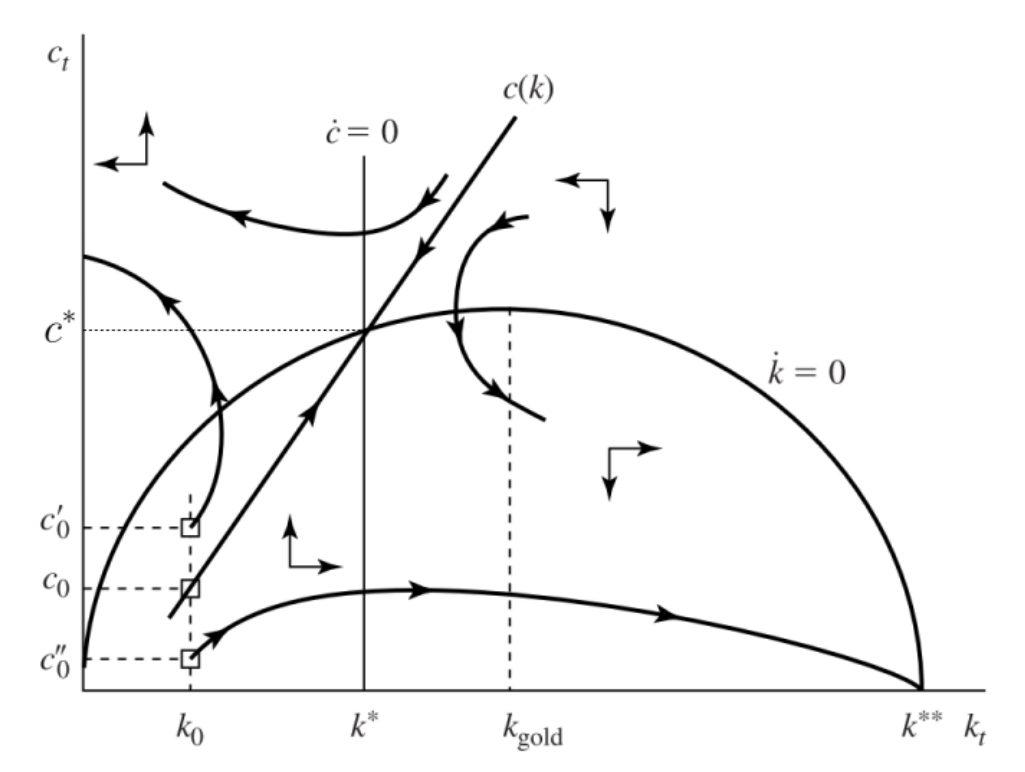
\includegraphics[width = 1 \textwidth]{./figures/RCK_phase_space.png}
  \end{minipage}\hfill

\end{figure}
From a physicist's perspective, eqs. \eqref{eq:kdot} and \eqref{eq:ramsey_keynes} resemble a system of ordinary differential equations that describe the dynamics of the RCK model in the $(k,~c)$ phase space. This line of reasoning would yield a phase space diagram like the one presented in fig.~\ref{fig:rck_phase_space} that exhibits trivial absorbing states along the axes $k=0$ and $c=0$ and two saddle points for $k=c=0$ and another one derived in eq. \eqref{eq:rck_steady_state}.
This view has some appeal as it allows for the framing of bubbles and crashes as deviations from the optimality curve and subsequent corrections to get back to it --- so much so that even economic textbooks feature figures like fig. \ref{fig:rck_phase_space} that clearly buy into this framing.
However, a closer look at the derivation of equation \eqref{eq:ramsey_keynes} reveals that this framing --- as attractive and intuitive as it seems --- is the product of circular reasoning and a flawed understanding of the mathematical optimization methods that are used to derive it. Particularly, the derivation of eq.~\eqref{eq:ramsey_keynes} is done by solving the intertemporal optimization problem posed by eq.~\eqref{eq:int1} subject to eq.~\eqref{eq:kdot} with eq.~\eqref{eq:NPG} with strict equality as a constraint. This constraint confines the solution of the optimization problem to the saddle point manifold in fig.~\ref{fig:rck_phase_space} which in return means that any discussion of this solution outside the saddle point manifold is meaningless. Consequently, any interpretation of the possible dynamics of equations \eqref{eq:kdot} and \eqref{eq:ramsey_keynes} that revolve around stability of the steady state, deviations from the manyfold and possible ways to return to it are meaningless as they are outside the support for which the ordinary differential equations were derived in the first place.

To sum up, this means that while the RCK model has been used extensively to study the effect of different policy measures on economic growth, its use for the study of non-equilibrium economic dynamics is somewhat limited. \\

An interesting extension of this model including heterogeneous agents and relaxing the rationality assumptions for their behavior can address this point. Subsequently, I introduce such a model.




\section{An Agent-Based Version of the RCK Model}
\label{sec:savings_model}
\subsection{Economic Model}
The model introduced in this chapter originated as a derivative and modification of the model described in section \ref{sec:heuristics_model}. The aim of this model is to answer some of the questions that I raised at the end of the previous chapter; namely, what effects may araise from heterogeneous agents individually setting their savings rates according to a simple social learning rule. In the following, I will explain the model in detail.\\

I introduce a heterogeneous agent model in the tradition of agent-based modeling \citep{LeBaron1999,Berry2002,Epstein2006,Dosi2010, Dawid2014,Hommes2018,Simon2018},
using agents that follow a very simple behavioral rule.  
This model contains $N$ households labeled by $i$ with heterogenous capital $K_i$. For simplicity, all households supply the same labor $L_i = L/N$.  \footnote{Introducing heterogeneous labor has little effect on the results}.
As in the original RCK model, total economic production is given by the Cobb--Douglas production function, in this case applied to the aggregate input factors $K = \sum_{i=1}^N K_i$ and $L = N L_i$.
As in the original model, capital returns $r$ and wages $w$ equal marginal returns according to eq.~\eqref{eq:capital_rents},
but incomes $I_i$ now differ between households,
\begin{equation}
\label{eq:Ii}
	I_i = r K_i + w L/N.
\end{equation}

The key assumption is that each household individually and dynamically sets its time-dependent savings rate $s_i(t)$ according to a behavioral decision rule introduced below,
leading to household capital dynamics
\begin{equation}
	\dot{K}_i = s_i I_i - \delta K_i = (r s_i - \delta) K_i + w s_i L/N.
        \label{eq:rcka_kdot}
\end{equation}
At the steady state where $\dot{K}_i = 0$, the steady state value $K_i^*$ for household $i$'s capital is a function of the aggregate capital $K$ via its dependence on $w$ and $r$, 
nonlinearly interconnecting all the agents' savings rates and consumption levels.

\subsection{Household Decision Making}
While the standard RCK model is a one-dimensional dynamical system in which consumption is a deterministic function of the total capital, the agent-based version is $N$-dimensional, and aggregate consumption depends on all households.
I assume that each household updates its savings rate at random times\footnote{
%
This leads to smoother transitions than synchronous updates \citep{Vizzari2005, Fates2010}.
}
%
according to a Poisson process with rate $1/\tau$.

Households are embedded in a social network in which each household $i$ has neighbors $\mathcal{N}(i)$. Inspired by a recent study on heuristic behavior in social learning by \cite{Barkoczi2016}, I implement household behavior in the following way: Whenever household $i$ updates its savings rate, it compares the consumption rates of its neighbors and applies the `imitate-the-best' heuristic, copying the savings rate of the neighbor with the highest current consumption with a small deviation that can either be interpreted as an error or as an exploration \citep{Mehlhorn2015}. More precisely, when the consumption of a neighbor is higher, it adopts a new savings rate of
\begin{equation} 
	s^\mathrm{new}_i = s_{\underset{j\in \mathcal{N}(i)}\argmax_{} (C_j)} + \epsilon,
\end{equation}
where $\epsilon$ is distributed uniformly in the interval of $\pm 1\%$\footnote{With $\varepsilon=0$ the values of the savings rate the households can use are confined to the values that occur in the initial condition. Also, values of the savings rate can ``die out'' as soon as the last household has abandoned them. This leads to strong and artificial path dependencies. The model behavior is insensitive to to exact value of $\varepsilon$ as long as there is some diversity e.g. $\varepsilon>0$}.
Note that in this model household savings rates are strictly non-negative. While this excludes effects that may come from borrowing between households, it  also serves as a simple and robust alternative for the No-Ponzi-Game condition that lies at the heart of the original RCK model. 

\subsection{Simulation Details}

For the simulations that are presented in the subsequent results section, the parameters and initial conditions are as follows if not explicitly stated otherwise:
$L_i = 1/N, K(t=0)_i \!= \!1 \forall\,\, i$ and a fully connected network with $N=100$, $\delta=0.05$. We have found that adding small heterogeneity in each household's labor does not change the dynamics significantly and the equilibrium dynamics also remain the same for different initial capital distributions with different $\sum_i K_i = K$. We used Gillespie's algorithm \citep{Gillespie1977} to simulate the stochastic trajectory.

\section{Results}
\label{sec:savings_results}
I present the results as follows: First I show the model dynamics depending on the mean social interaction time $\tau$ and classify them according to two qualitatively different regions. I consecutively analyze these two regions with respect to their dynamic properties and explain the underlying mechanisms. Finally, I explain the origin of the critical social interaction time that separates the different dynamical regimes and discuss its dependency on the structure of the interaction network.\\
\begin{figure}[ht]
     \centering
     \vspace{-.2 cm}
     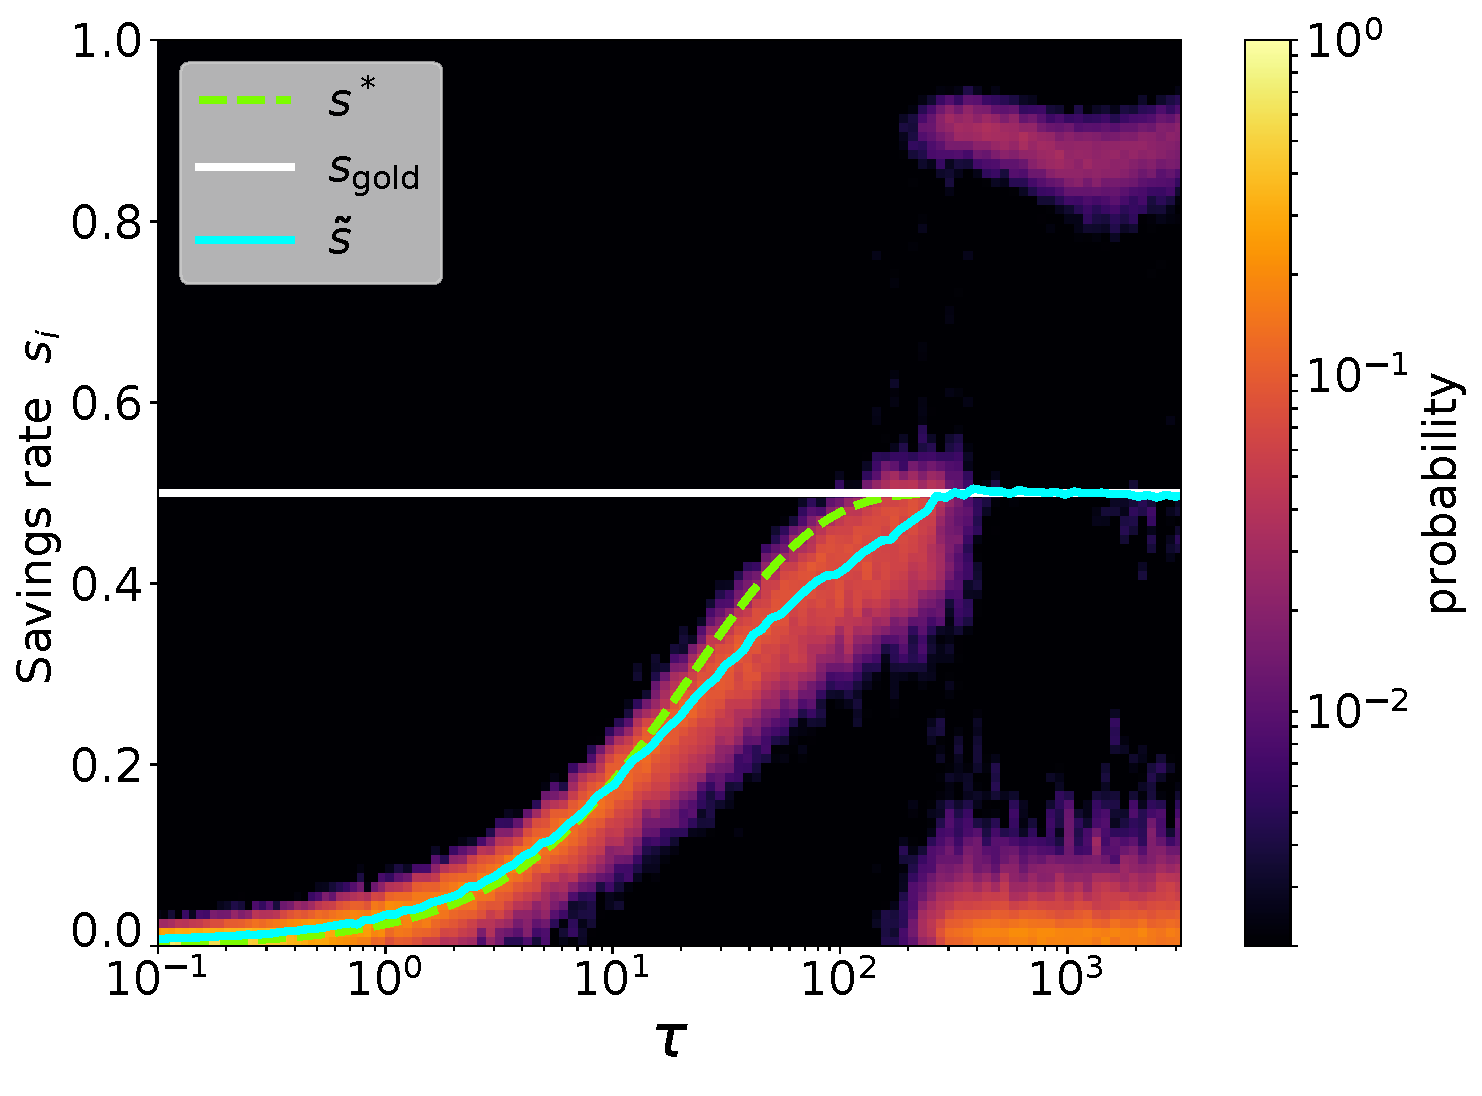
\includegraphics[width=.9\linewidth]{figures/fig1.pdf}
     \caption[Distribution of individual savings rates depending on the social interaction rate]{\textbf{ The critical transition from the stable regime to the oscillatory regime.} 
	 Results from an ensemble of simulations at different values of the social interaction time $\tau$, with other parameters held fixed. The savings rate distributions are shown at the final state of the simulation at time $5\tau \times 10^3$, far beyond the point where the model has reached its asymptotic dynamics. For each value of $\tau$, $200$ independent simulations are run and all values of $s_i$ are recorded for each $\tau$ to construct a normalized histogram.
       The heatmap indicates the probability density of the distribution of individual households savings rates for each value of $\tau$, along with the aggregate savings rate $\tilde{s}$. This is compared to the golden rule savings rate $s_\mathrm{gold} \! = 0.5$ and the savings rate $s^*$ predicted by eq.~(\ref{eq:s_optimal}).}
	
   \label{phase}
\end{figure}
We simulated the model for a variety of different parameters such as the average social interaction time $\tau$ and the network topology. Fig.\,\ref{phase} shows the distribution of the final savings rates as a function of the mean social interaction time $\tau$ for a complete network with the remaining parameters fixed.  The figure compares this result to the optimal, `golden rule' savings rate $s_\mathrm{gold}$,  corresponding to the rational expectations equilibrium where the consumption of the representative agent is maximized. For comparison, the figure also shows the analytical approximation of the steady state savings rate of the model $s^*$ in eq. \eqref{eq:s_optimal}.\\

These results clearly show that there are two distinct regimes, separated by a critical social interaction time $\tau_{c} \approx 250$.
In the \emph{stable regime}, corresponding to $\tau < \tau_{c}$, the savings rates of the households are unimodally distributed around a low savings rate.  For very small values of $\tau$ the savings rates are close to zero, and because of this, the economy is stuck in a poverty trap in which its output is very low.  As $\tau$ increases, the savings rate and output increase, but the distribution remains unimodal, with a sub-optimal aggregate savings rate.

For $\tau \! > \! \tau_{c}$ the economy enters what I call the \emph{ oscillatory regime}, where the behavior is dramatically different. In this regime the savings rate distribution is bimodal --- some households have high savings rates and are :``wealthy'', while others have low savings rates and are ``poor''.  Thus, this model exhibits spontaneous emergence of extreme inequality, with a lower class and an upper class.

Very near $\tau_\mathrm{c}$ the distribution in fig.~\ref{phase} becomes tri-modal. This is due to intermittent oscillations between the unimodal and bi-modal regimes. Thus the system either exhibits a middle class, or a lower class and an upper class, but never all three at once.

Strikingly, as long as $\tau \! > \! \tau_{c}$, the ensemble average of the observed economy wide aggregate savings rate $\tilde{s}$ is within $1\%$ of the optimal value $s_\mathrm{gold}=\alpha=0.5$, even when the individual distributions are bimodal.
Furthermore, the time averages of total economic output $Y(t) \!=\! 10.15$ and  consumption $C \! = \! 4.99$ are close to their optimal values $Y^\ast \! = \! s_\mathrm{gold} L/\delta \! = \! 10$  and $C^\ast \! = \! (1-s_\mathrm{gold})Y^\ast \! = \! 5$  in the standard RCK model.  It is surprising that such a simple, near zero-intelligence learning rule can maintain the system this close to its optimal behavior.
\begin{figure}[t]
     \centering
       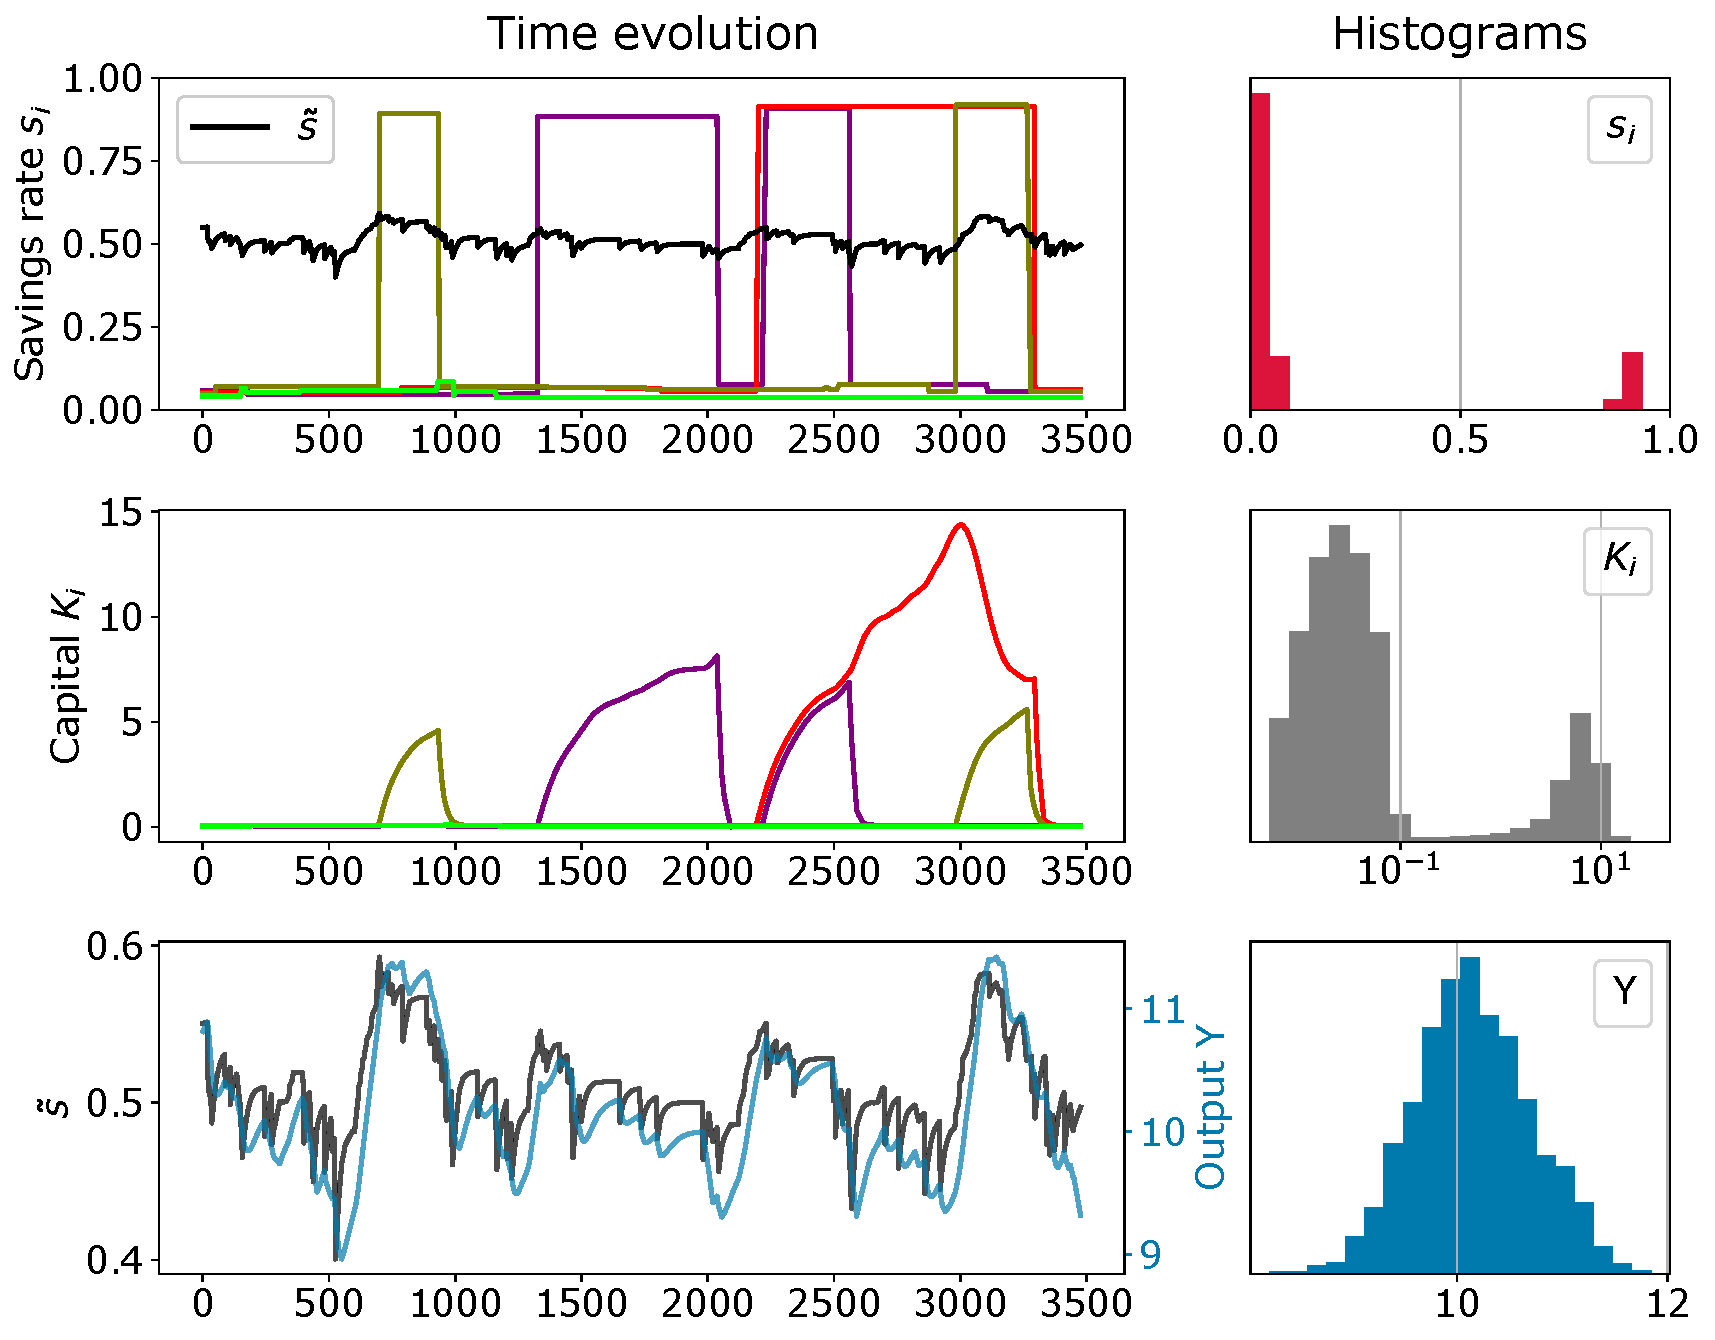
\includegraphics[width=0.99\linewidth]
       {figures/fig2.pdf}
       \caption[Trajectory of individual and collective oscillations in savings rates and economic output]{\textbf{ The endogenous business cycle in the oscillatory regime}.   I show several time series for $\tau \!>\! \tau_\mathrm{c}$.  
	The top left panel shows the savings rates $s_i(t)$ for randomly chosen households as a function of time, as well as the aggregate savings rate $\tilde{s}$.  
	The middle left panel shows the capital $K_i(t)$ of the same households as a function of time. The bottom left panel shows the cyclic behavior of the aggregate output superimposed on the aggregate savings rate.  The panels on the right are histograms of the indicated variables, accumulated over a longer interval.}
   \label{fig:micro_trajs}
\end{figure}

The system dynamics become clearer when analyzing the properties of the 
economy as a function of time, as illustrated in fig.~\ref{fig:micro_trajs}.  
For $\tau \! > \! \tau_\mathrm{c}$ there is an endogenous oscillation in many of the aggregate properties of the economy, including the aggregate savings rate $\tilde{s}(t)$ and output $Y(t)$.  This oscillation is also visible in the behavior of individual households.  If one follows any single household it experiences epochs with both, a high savings rate near $s_i \! \approx \! 0.90$, and a low savings rate near $s_i \! \approx \! 0.05$.  At any point in time there is typically an imbalance between rich households and poor households, so that the aggregate savings rate and the aggregate output fluctuate.  I loosely refer to this endogenous oscillation as a ``business cycle''.
%In the Supplementary Information (SI) we show that the value of the high savings rate varies between $65\%$--$90\%$ depending on the topology of the network.  


\subsection{Understanding the Stable Regime ($\mathbf{\tau \! < \! \tau_{c} }$)}
\label{sec:savings_stable}
Although the behavioral rule of the `imitate-the-best' heuristic requires minimal intelligence, the selection process of copying the household with the highest consumption provides a simple mechanism of collective search that becomes more effective as the social updating time $\tau$ increases.  This is perhaps counter-intuitive, as it means that inattention results in superior collective outcomes. The underlying explanation is as follows:  The  savings rate of the household that is copied has on average been fixed for a time interval of order $\tau$. When $\tau$ is small, planning is too myopic, ``short term thinking'' dominates, and the households cannot escape using low savings rates with high consumption.  As $\tau$ increases, however, the time between updates becomes long enough that there is more time to accrue an advantage by saving. This drives the savings rate up and increases economic output. The competitive selection process guarantees that for a sufficiently large population and large $\tau$ the savings rates are close to optimal. This is similar to the behavior of a model of local resource exploitation \citep{Wiedermann2015}.

We can use this intuition to derive an approximate formula for the aggregate savings rate $s^*$ as a function of~$\tau$. This derivation takes advantage of the fact that in the stable regime the distribution is unimodal and assumes that all households have essentially the same savings rate. With this, one can derive the optimal savings rate for time horizon $\tau$ as follows.\\ 

\subsubsection{Analytical Approximation of the Stable Regime's Steady State}
\label{sec:rck_stable}
The main idea is the following: First, study which member of an ensemble of households  will have the largest consumption after the short time interval $\tau$ given that they all start at similar but slightly different savings rates. Then, assume all households will copy the savings rate of this best household with some error. 
This is only an approximation since in the actual model, households do not simultaneously imitate each other after an exact time $\tau$. Furthermore, the approximation will only be satisfactory when households have already converged to similar savings rates and capital stocks.
Nevertheless, the approximation describes the joint motion towards a steady state  rather well once households have converged towards each other.

To see how individual households' consumption at time $\tau$ depends on their individual savings rate, one has to approximate the evolution of $r$ and thus of total capital $K$ first. Let us assume that all households' savings rates $s_i$ are close to the overall savings rate $s$ and stay constant between time zero and time $\tau$. 
Then according to eq. \eqref{eq:rcka_kdot} $K$ evolves as 
\begin{equation}
    \begin{split}
    \dot K &= (r s - \delta) K + w s L \nonumber \\
    	   &= \Big(\alpha\Big(\frac{L}{K}\Big)^{1-\alpha} s - \delta\Big) K + \alpha \Big(\frac{K}{L}\Big)^{1-\alpha} s L.  
	\end{split}
\end{equation}
For $\alpha = 1/2$ this simplifies to 
\begin{equation}
    \label{aggKdotnew}
    \dot{K} = s\sqrt{L K} - \delta K.
\end{equation}
Assuming that $s$ does not change before time $\tau$, this can be solved via separation of variables which results in two solutions given by 
\begin{equation}
\begin{split}
    K(t) &= \Big(\frac{B - E e^{-\delta t/2}}{\delta} \Big)^2, \\
    r(t) &= \sqrt{L/K} / 2 = \frac{A}{B - E e^{-\delta t/2}}, \\
    w(t) &= \sqrt{K/L} / 2 = \frac{B - E e^{-\delta t/2}}{4 A}
\end{split}
\end{equation}
for all $t < \tau$,
where 
$A = \delta \sqrt{L} / 2$,
$B = s\sqrt{L}$,
and
$E$ has the two possible values $s\sqrt{L} \pm \delta \sqrt{K_0}$.
Since the only relevant solution is that in which $r$ is positive, we find $E = s\sqrt{L} - \delta \sqrt{K_0} < B$.

Knowing $r(t)$ and $w(t)$, we can now determine which household consumes most after time $\tau$.
Household $i$'s capital $K_i(t)$ evolves as 
\begin{equation}
\begin{split}
    \dot K_i 
    &= (s_i r(t) - \delta) K_i + w s_i L_i \nonumber \\
    &= \left(\frac{A}{B - E e^{-\delta t/2}} - \delta\right)s_i K_i
        + \frac{B - E e^{-\delta t/2}}{4 A} s_i L_i.
\end{split}
\end{equation}
This has an analytical solution involving complicated hypergeometric functions.
For small values of $\tau$, we can simplify the problem by approximating $r(t)$ and $w(t)$ for $t\in[0,\tau]$ by their mid-term values $r(\tau/2)$ and $w(\tau/2)$, giving
\begin{equation*}
\dot{K_i} \approx G_i K_i + F_i
\end{equation*}
with $G_i = \frac{s_i A}{B - E e^{-\delta \tau/4}} - \delta$
and $F_i = \frac{B - E e^{-\delta \tau/4}}{4 A} s_i L_i$,
which solves as
\begin{equation*}
    K_i(t) \approx (K_i(0) + F_i/G_i)e^{G_i t} - F_i/G_i.
\end{equation*}
The corresponding consumption of household $i$ at time $\tau$ is then
\begin{align}
    C_i(\tau) 
    &= (1 - s_i)(r(\tau) K_i(\tau) + w(\tau) L_i) \nonumber \\
    &\approx (1 - s_i)\left( 
        H((K_i(0) + F_i/G_i)e^{G_i\tau} - F_i/G_i)
        + L_i/4 H
    \right)
\label{eq:Citau}
\end{align}
with 
\begin{equation}
        H = \frac{A}{B - E e^{-\delta\tau/2}} = \frac{A}{s\sqrt L (1 - e^{-\delta\tau/2}) + \delta \sqrt{K_0} e^{-\delta\tau/2}}.\nonumber
\end{equation}
%Note that $F_i/G_i$ decreases as $s_i$ increases.
We assumed that at time $\tau$ all households imitate the savings rate $s_i$ that has led to the largest $C_i(\tau)$. This means that as long as a single household can increase its consumption $C_i(\tau)$ by choosing a savings rate $s_i$ that is similar to but different from $s$, all households will imitate this savings (with some error) rate and the aggregate savings rate will move towards $s_i$. 
We can also determine whether $s$ will increase or decrease by identifying whether the $s_i$ that gets copied is larger or smaller than $s$.
Since we also assume households' savings rates $s_i$ are distributed closely around $s$, and that all $K_i(0), L_i$ are similar, this can be determined by seeing whether $C_i(\tau)$ increases or decreases when $s_i$ is increased from below $s$ to above $s$, i.e., by studying the derivative $\partial C_i(\tau)/\partial s_i$ at the point $s_i = s$. Up to a factor of $N$, this derivative is given by
\begin{align}
  \frac{\partial C_i(\tau)}{\partial s_i} = &(1 - s) H\left[
        \frac{e^{G\tau} - 1}{G}(L / 4 H - H F/G) + e^{G\tau}\tau H (K_0 + F/G)\right] \nonumber \\
    &- H[(e^{G\tau} - 1) F/G + e^{G\tau} K_0] 
    - L / 4 H
    \label{sdotnew}
\end{align}
where
$F = \frac{B - E e^{-\delta \tau/4}}{4 A} s L$
and
$G = \frac{s A}{B - E e^{-\delta \tau/4}} - \delta$.
As long as the above expression is positive or negative, $s$ will increase or decrease over time, respectively.

A steady state will then be reached when both $s$ and $K$ change no longer, i.e., when both $\dot K$ as given by eq.~\eqref{aggKdotnew} (with $K=K_0$) as well as $\partial C_i(\tau)/\partial s_i$ as given by eq.~\eqref{sdotnew}
vanish.
The solution of $\dot K = 0$ is 
$K_0 = L s^2 / \delta^2$, 
at which point we have
$E = 0$,
$H = \delta / 2 s$, 
$G = - \delta / 2$, 
$F/G = - L s^2 / \delta^2 = - K_0$, 
$H K_0 = L s / 2 \delta$, and
$H F / G = - L s / 2 \delta = - H K_0$.
Substituting all this into eq.\,\eqref{sdotnew} and equating it with zero gives the following surprisingly equation for the steady state $s$:

\begin{equation}
\label{eq:s_optimal}
s^\ast(\tau) = \frac{1 - e^{-\delta \tau/2}}{2 - e^{-\delta \tau/2}}.
\end{equation}
This approximation describes the aggregate macroscopic behavior of the model in the stable regime. It illustrates that this macroscopic behavior is determined by the relative time scales of the two major processes in this model, the capital depreciation rate $\delta$ in the economic system that determines the transient dynamics of capital accumulation through savings and the social interaction time $\tau$ that determines the speed of collective search in the social learning process. Such behavior is common for many coupled dynamical systems. [Maybe some citations here.] This approximation is shown in green in fig.~\ref{phase} comparing it to the aggregate savings rate and the distribution of individual savings rates from numerical simulations. This shows that this analytical approximation provides a good fit of the aggregate savings rate throughout the stable regime.

The analytical approximation of the aggregate savings rate in the stable regime of the agent-based RCK model can be compared to the optimal savings rate in the steady state of the standard RCK model. In the standard RCK model as given in eq.~\eqref{eq:rck_steady_state}, the optimal savings rate depends on the capital depreciation rate $\delta$ and the discount rate $\rho$, which is a free parameter. Substituting $s^\ast$ from eq.~\eqref{eq:s_optimal} into the relation for the classical RCK model from eq. \eqref{eq:rck_steady_state} and solving for $\rho$ gives an effective discounting rate for this model in terms of the social interaction time $\tau$ and the depreciation rate $\delta$,
\begin{equation}
   \rho(\tau) = \frac{\delta/2}{e^{\delta \tau/2} - 1}. \label{eq:rhotau}
\end{equation}
In the limit of $\tau \to 0$, the discount rate $\rho$ diverges, consistent with the observed collectively myopic behavior. But for $\tau \to \infty$, the discount rate $\rho$ converges to zero consistent with collectively farsighted behavior and an optimal savings rate in the sense that this would be the savings rate that a social planner would choose to achieve the highest sustainable aggregate consumption. Thus in this case the individually myopic households act collectively ``as if'' they were farsighted, with an emergent effective discounting rate $\rho(\tau)$ which is not a free parameter but is rather a function of the social interaction time $\tau$. Similar emergent behavior has been found in the interaction of adaptive voter type social learning with individual management of renewable resources where sustainable far sighted management of the resource is possible when the interaction time in the social learning process is sufficiently large compared to the time scale of the inherent dynamic renewable resource \citep{Wiedermann2015}. 


\subsection{Understanding the oscillatory regime ($\mathbf{\tau \!>\! \tau_{c} }$)}
\label{sec:savings_oscillations}
\begin{figure}[t]
     \centering
       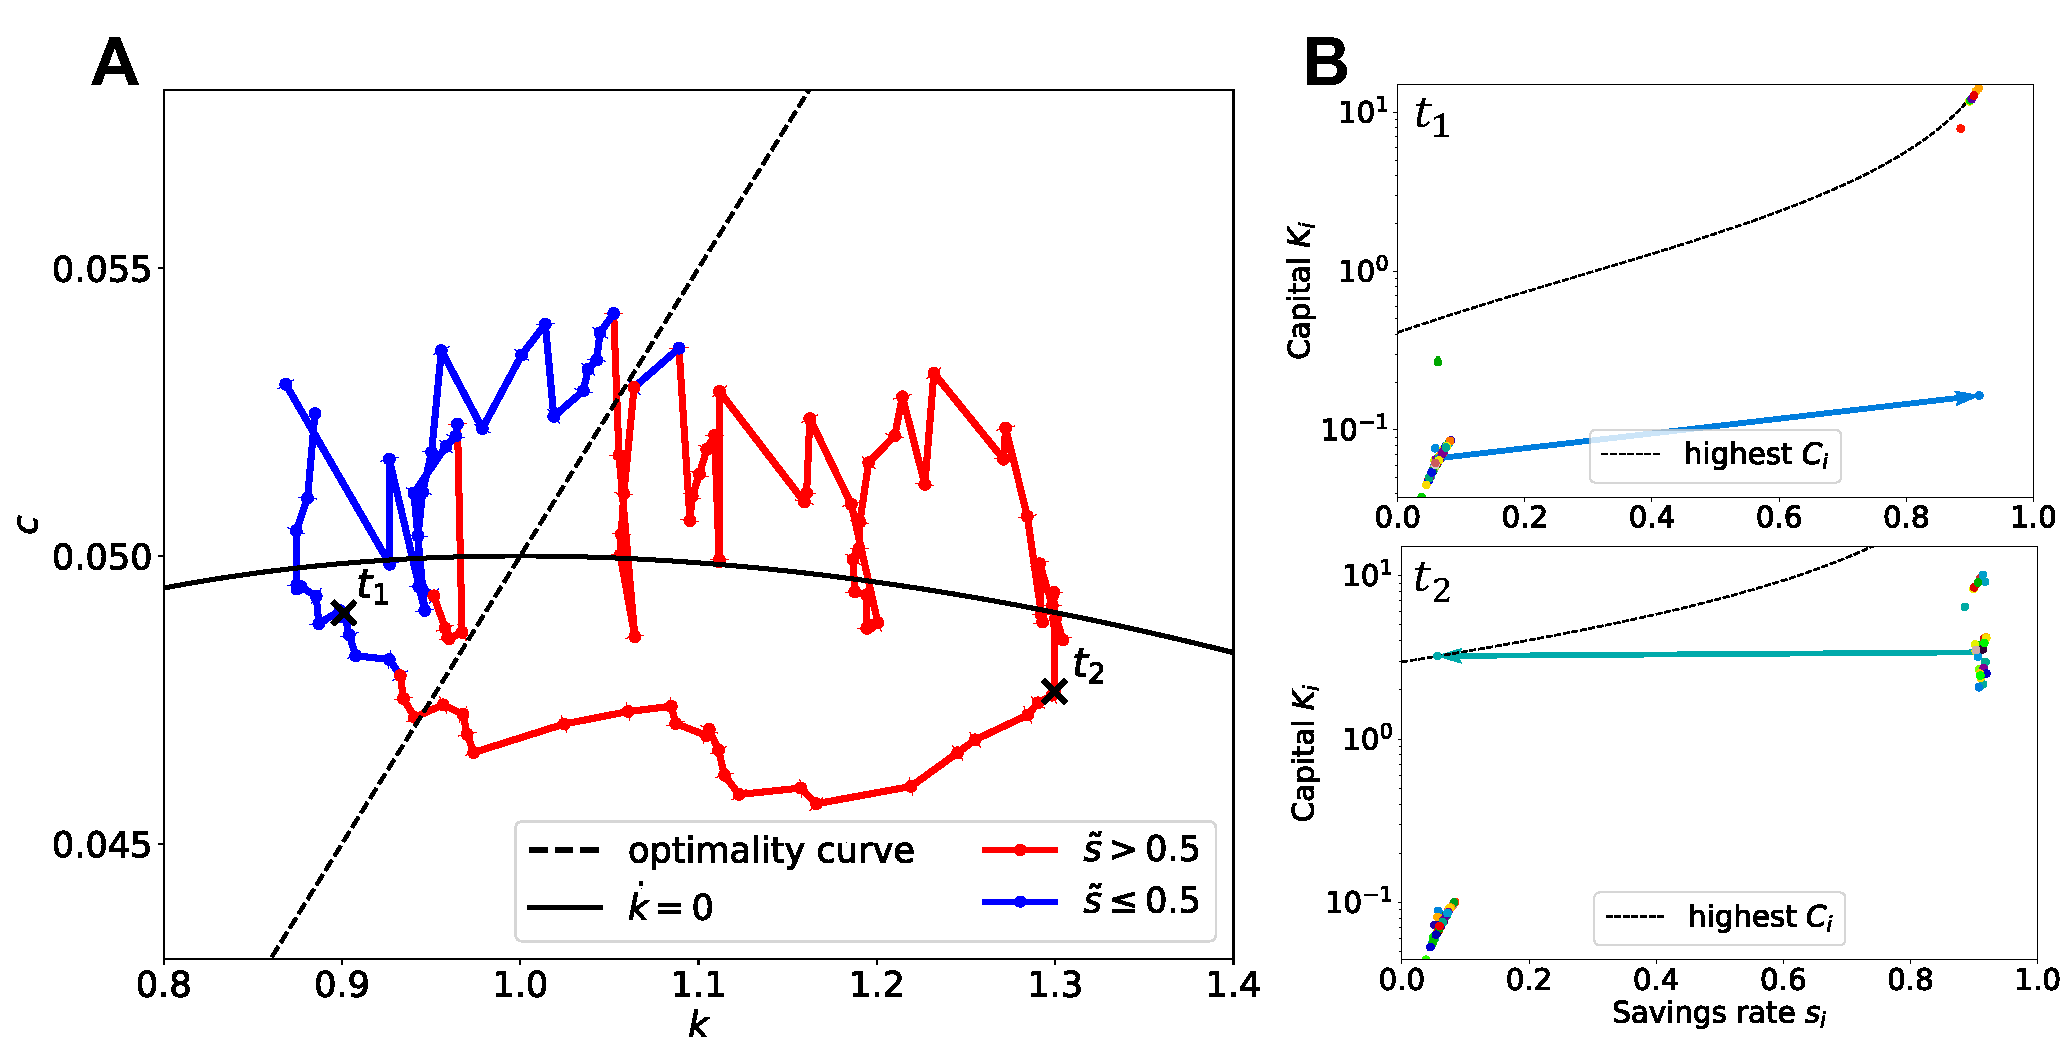
\includegraphics[width=0.98\textwidth]
       {figures/fig3.pdf}
       \caption[Endogenous dynamics in the oscillatory regime]{\textbf{ Endogenous dynamics in the oscillatory regime. } \textbf{A}: the average per-capita consumption $c$ against the average per-capita capital $k$. The aggregate saving rate $\tilde{s}$ is red when it is greater than $0.5$ and blue when it is less than $0.5$. The trajectory orbits around the optimal steady state $(k^\ast,c^\ast)$  of the standard RCK model, which is at the intersection of the dashed optimality curve (the solution to the standard RCK model discussed in sec.~\ref{sec:rck_stable}) and the solid black $\dot{k}=0$ line. Each dot corresponds to one household updating its savings rate; the direction of the orbit is counterclockwise.
\textbf{B}:~An illustration of the cause of the oscillatory dynamics.  The two panels show snapshots at two different times as indicated in figure A.  At time $t_1$ the aggregate savings rate is low, aggregate capital is low and the economy is in a depression; at time $t_2$ the opposite is true.  The capital and savings rates of individual households are shown as dots with different colors.  There are two clusters, corresponding to rich and poor households.  The household that is currently switching its savings rate is indicated by an arrow connecting its previous state to its current state.  The dashed black curve indicates the iso-consumption curve for the household $i$ with the highest consumption. }
\label{fig:dynamics}
\end{figure} 
In order to obtain a deeper understanding of the oscillatory regime, where $\tau > \tau_{c}$, fig.~\ref{fig:dynamics} illustrates both collective and individual dynamics.

Fig.\,\ref{fig:dynamics}A shows the average per capita consumption rate $c$ as a function of the average capital $k$. 
This illustrates how the aggregate consumption and capital orbit around the optimal steady state $(k^\ast,c^\ast)$  of the standard RCK model, generating a business cycle. 
The dashed line in fig.~\ref{fig:dynamics} represents the trajectory of the standard RCK model as discussed in sec.~\ref{sec:rck_stable}, the so called optimality curve, that is also depicted as the stable saddle point manifold in fig.~\ref{fig:rck_phase_space}.
In relation to the optimal savings rate $s^\ast \!=\!0.5$ of the RCK model, the effective aggregate savings rate $\tilde{s}$ of the modified model is typically greater than $s^\ast$ when the system is below the optimality curve and less than $ s^\ast$ when it is above the optimality curve. This means that when the heterogeneous households together have less capital than the representative household on the optimal trajectory, they increase their aggregate savings rate above the savings rate of the optimal scenario and vice versa, as if they were trying to collectively control their economy to steer it towards the optimal trajectory.
This is interesting as the optimality curve is obtained by assuming that a representative household optimizes its consumption for an infinite horizon, whereas in this modified model the individual household is oblivious of the mechanics of the economic system in which it operates and its behavior is myopic.

To understand the model mechanics at the individual level, fig.~\ref{fig:dynamics}B shows a snapshot of the capital vs.~the savings rate for all households at two different times, $t_1$ and $t_2$. 
At time $t_1$ the economy is just beginning to recover from a recession i.e. a period of low aggregate savings resulting in the depreciation of the capital stock and consequently lowered aggregate economic output. 
There are two clusters of households, corresponding to wealthy households with high capital $K_i$ and high savings rate $s_i$ and poor households with low capital $K_i$ and low savings rate $s_i$.
More households are poor, and because the return $r$ is inversely proportional to total capital according to $r \propto K^{-1 + \alpha}$, where here $\alpha = 0.5$, this means that returns to investment are high. 
As a consequence of this, wealthy households have a relatively higher consumption than poor households despite the fact that they save a large fraction of their income. This makes high savings rates comparatively more attractive than low savings rates. 
When the household shown in blue gets its chance to update its savings rate, it copies the higher savings rate of one of the rich households and moves in the $(K_i, s_i)$ plane as indicated by the arrow. Consequently, it begins accumulating capital by saving more.
Other households follow, and eventually the economy reaches the state shown in the lower panel at time $t_2$, where many houses have high savings rates and are rich.
The resulting excess capital drives the returns on savings down, which when combined with their high savings rates, depresses the consumption of these households.
As a result, when one of the rich households gets its turn to update, it copies a household with a low savings rate and goes on a spending spree.  

At this point its consumption rate becomes very high, and all of its neighbors copy it, creating a boom in consumption while decreasing the aggregate savings rate and consequently depreciating the capital stock of the economy.
A majority of households eventually become impoverished, returns on capital recover, high savings rates become more attractive again and the cycle repeats itself.
\subsection{Critical Social Interaction Time}
\label{sec:savings_critical_tau}
What determines the critical social interaction time $\tau_\mathrm{c}$?
This question can best be answered by a closer analysis of eq. \eqref{eq:Citau} which describes the consumption of an 
\begin{wrapfigure}[27]{o}{.6 \textwidth}
  \centering
  \hspace{-1.5cm}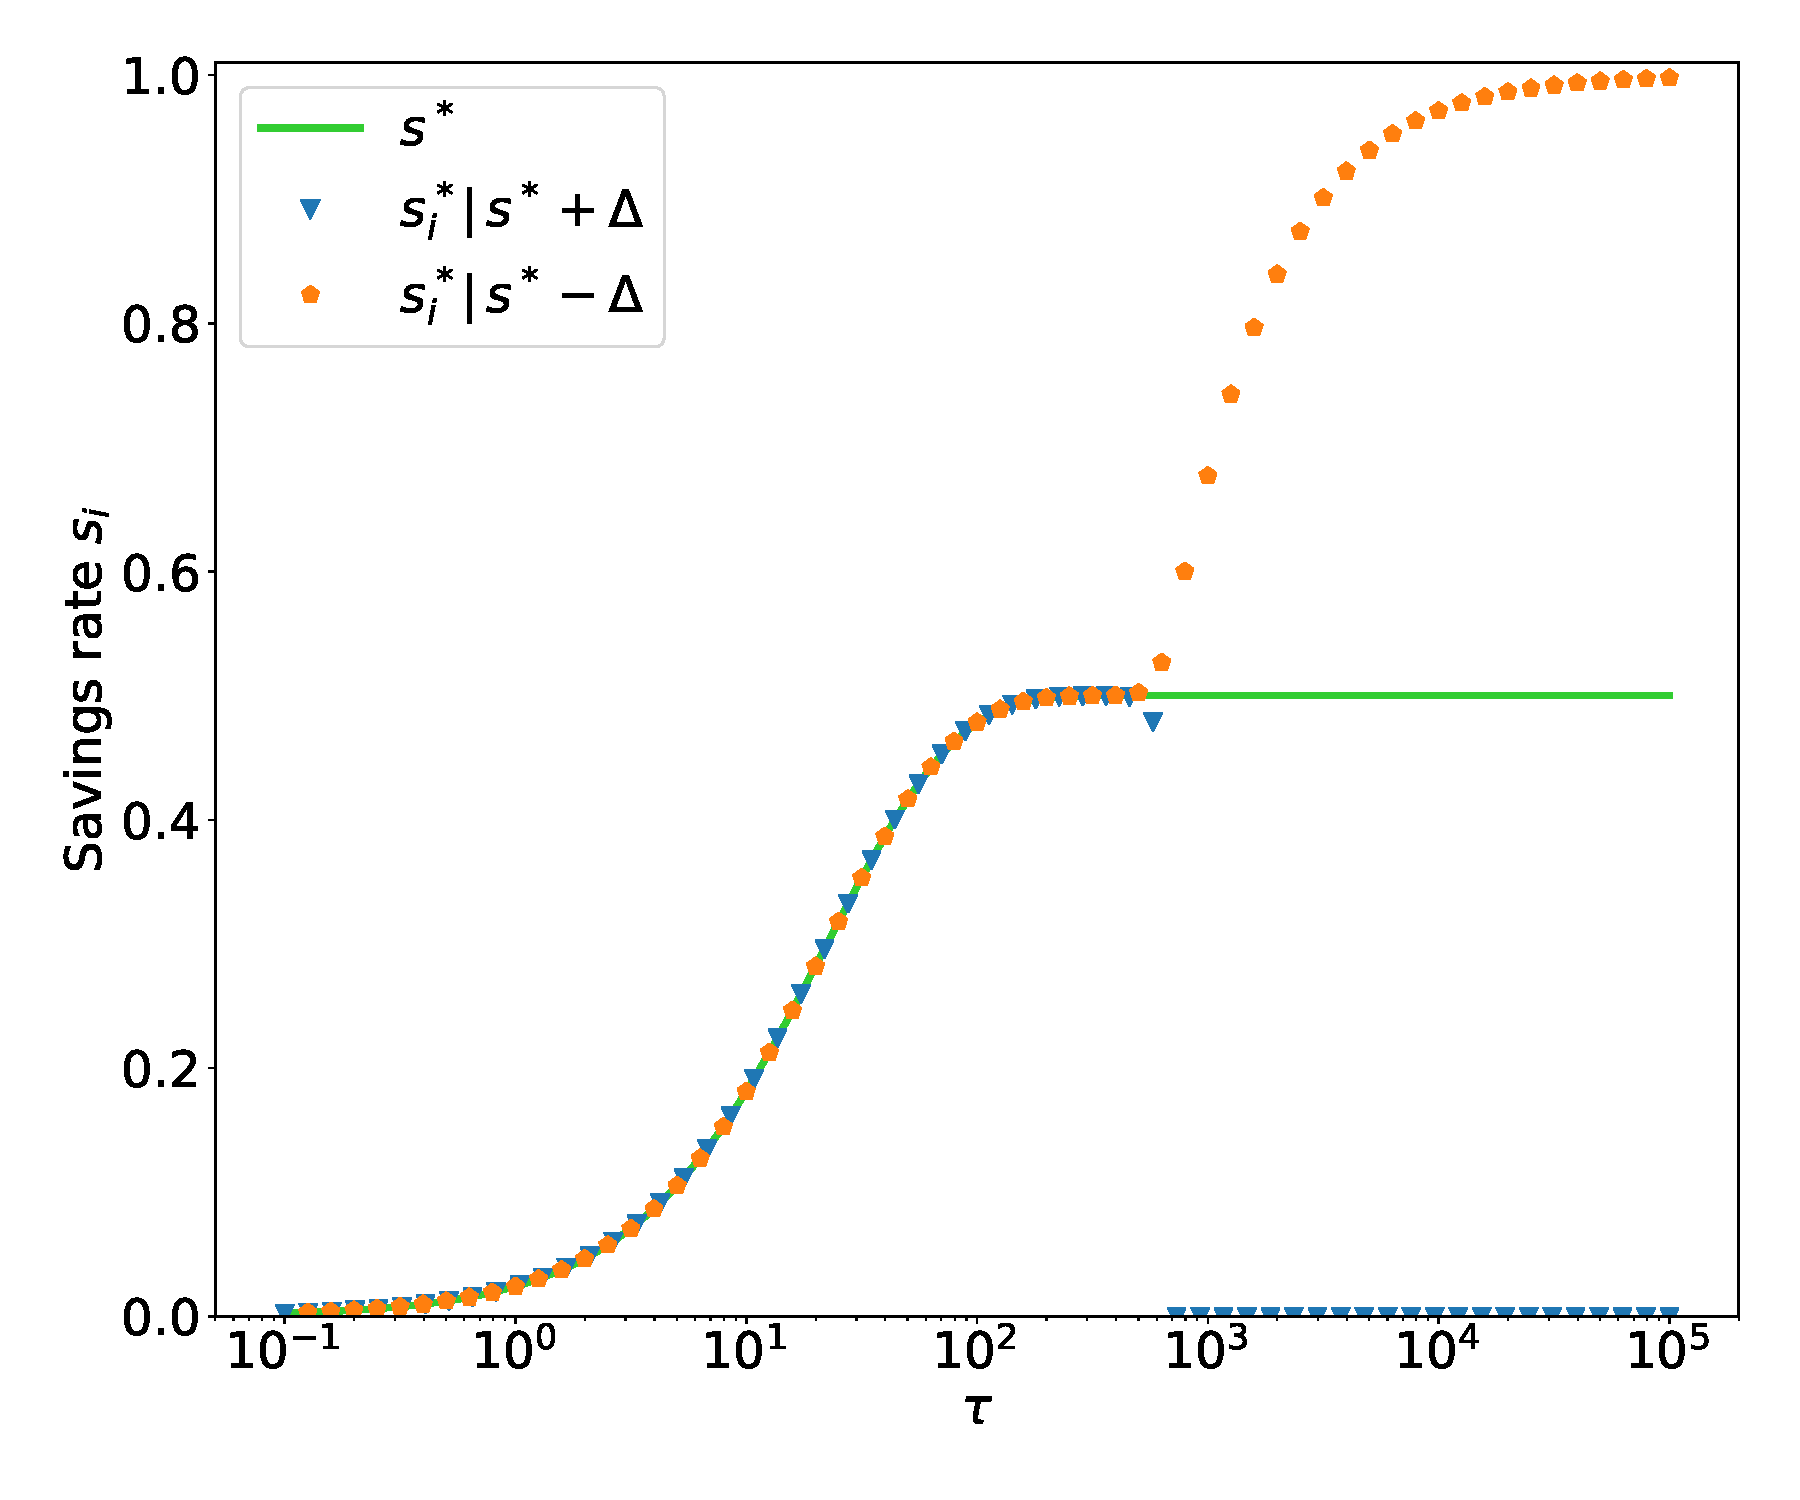
\includegraphics[width = .7 \textwidth]{figures/best_response.pdf}
  \caption[Best response dynamics for individuals savings rates]{Best response dynamics. Optimal individual savings rate $s_i^\star$ (circles and triangles) given a very small perturbation of either $+\Delta$ (blue circles) or $-\Delta$ (orange triangles) of the aggregate savings rate $s$ away from its equilibrium value $s^\star$ (green line) as a function of the social interaction time $\tau$, for $\Delta = 10^{-7}$.}\hspace{.5cm}
  \label{fig:best_response}
\end{wrapfigure}
 individual household after time $\tau$ given that this household sets its savings rate $s_i$ individually relative to the constant aggregate savings rate $\tilde{s}$.
In section \ref{sec:rck_stable}, the analysis of this approximate equation showed that the imitate-the-best heuristic can result in behavior that is collectively ``optimal'' over a time horizon $\tau$ as it maximizes aggregate consumption. 
The reasoning behind this analysis also helps to understand the instability driving the transition: Eq.~\eqref{eq:Citau} also determines the incentives of a single household to set its individual savings rate equal to, close to, or far from the aggregate savings rate to maximize its individual consumption. 
Suppose that an external shock of size $\Delta$ perturbs the aggregate savings rate $\tilde{s}$ away from its collectively optimal value $s^\ast$, and suppose that household $i$ is allowed to optimize its savings rate $s_i$ while the others hold theirs constant. 
I call this optimal savings rate $s^*_i$ the \emph{best response} of the individual household. 
As displayed in fig. \ref{fig:best_response}, a numerical investigation shows that when $\tau \ll \tau_{c}$ i.e. in the \emph{stable regime}, the best response $s^*_i$ that maximizes the individual household's consumption after $\tau$ remains close to $\tilde{s}$. 
In contrast, when  $\tau \gg \tau_{c}$ e.g. in the \emph{oscillatory regime}, if $\Delta > 0$ then the individual household's best response $s^*_i$ is very small, with $s_i$ approaching $0$, and if $\Delta < 0$ the optimal savings rate is large, with $s_i$ approaching $1$. 

This happens because when $\Delta > 0$ the aggregate savings rate is high, so the returns on investment are low, which discourages saving and vice versa, when $\Delta < 0$ the aggregate savings rate is low, so returns on investment are high, which encourages saving. 
This destabilizes the unimodal solution around $s^\ast$. 
The transition occurs sharply at a parameter value near $\tau_{c}$, though the precise value depends on $\Delta$.
\subsection{Dependence of the Critical Social Interaction Time on Network Size and Structure}  
\label{sec:savings_network_structure}

\begin{wrapfigure}[26]{I}{.6 \textwidth}
  \centering
  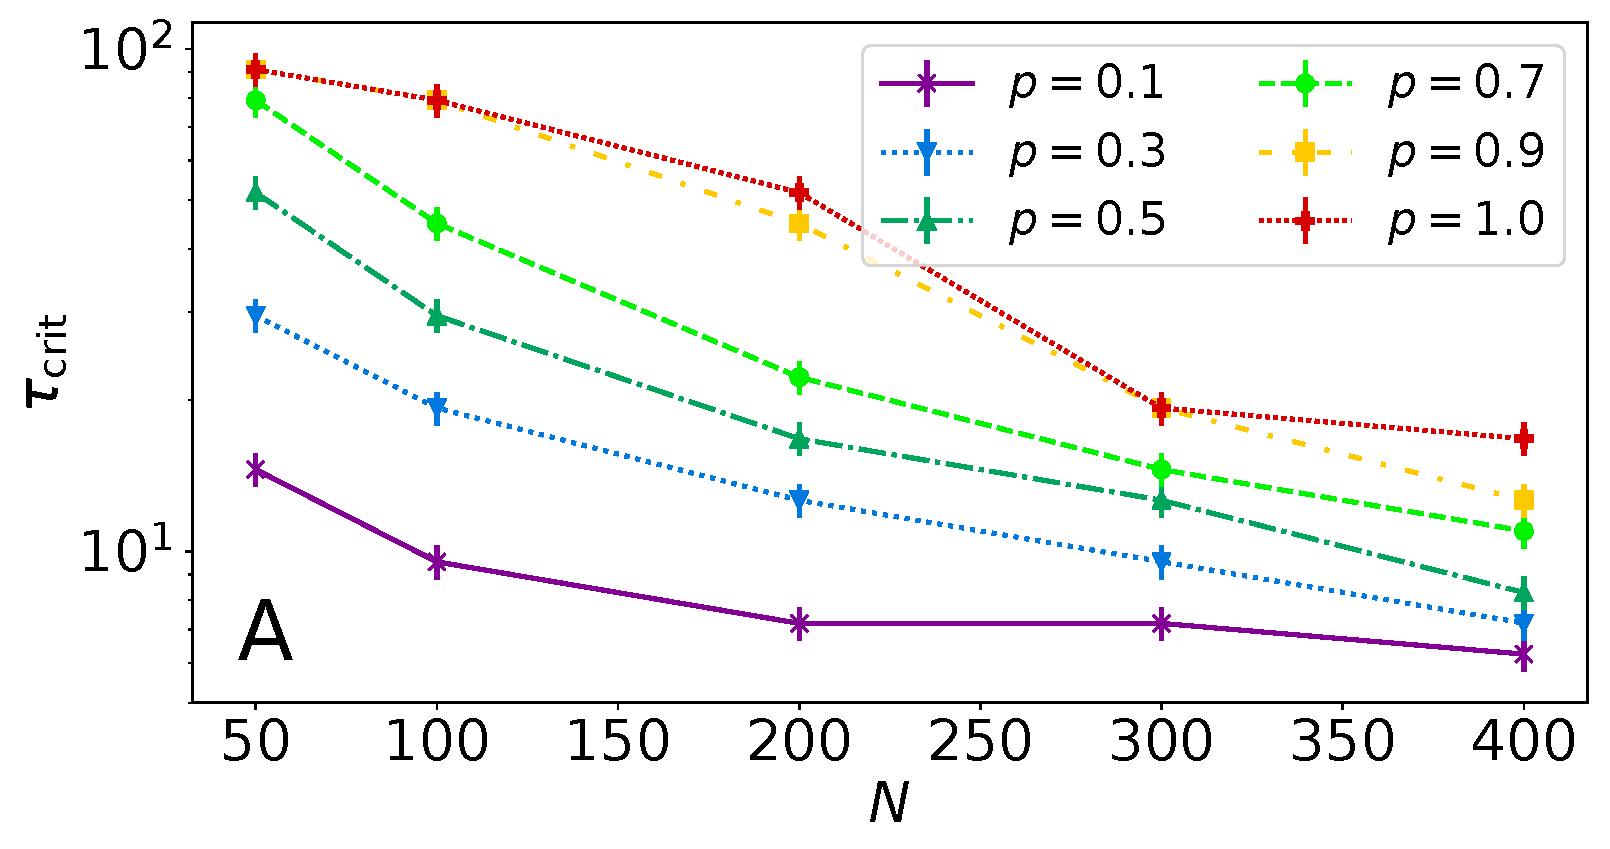
\includegraphics[width = .6 \textwidth]{figures/taucrit_N2.pdf}
  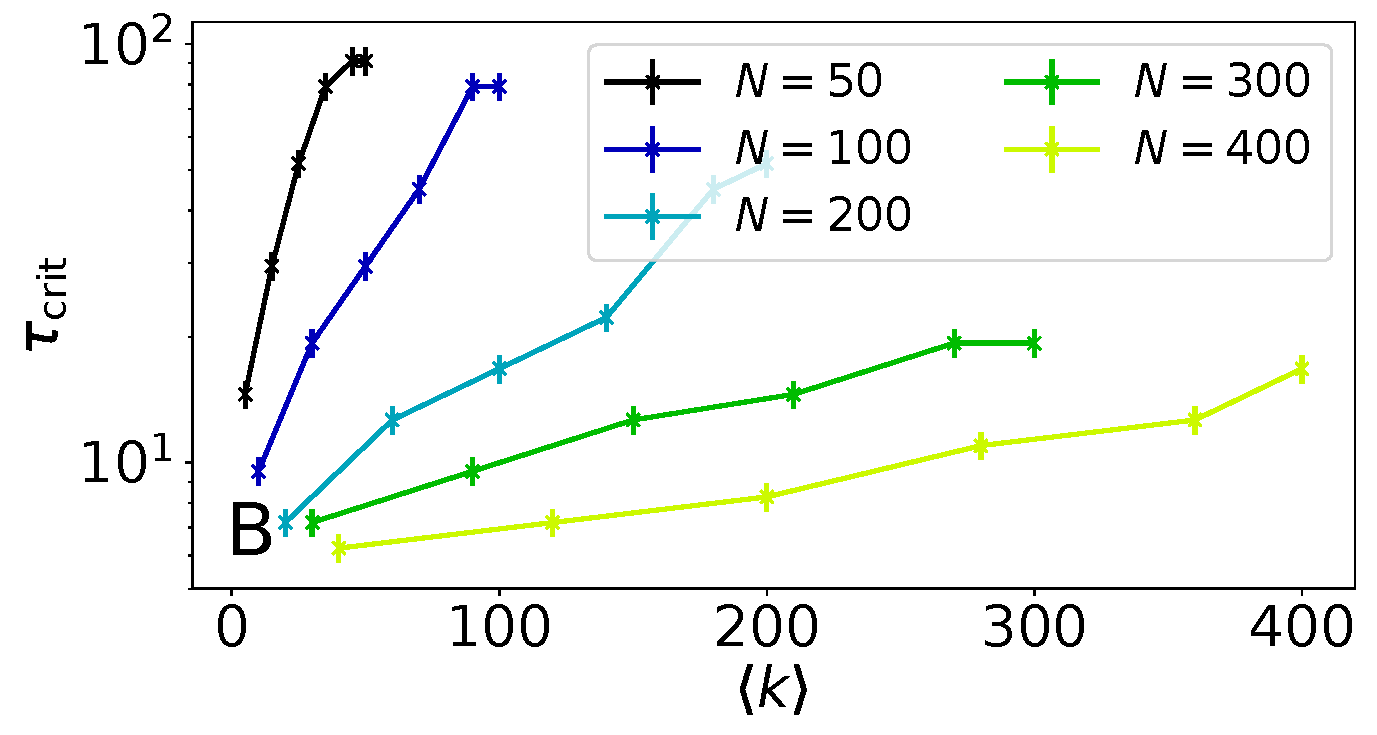
\includegraphics[width = .6 \textwidth]{figures/taucrit_N_k.pdf}
\caption[Critical interaction time depending on network size and mean degree]{Critical interaction time $\tau_{crit}$ depending on A) network size $N$ for different link densities $p$ of the Erd\H{o}s-Renyi graph and B) mean degree $\left< k \right>$ for different network sizes $N$.}
  \label{fig:taucrit}
\end{wrapfigure}
The analysis of the incentives for the individual household to set its savings rate close to or far from the collectively optimal value $s^*$ in section \ref{sec:savings_critical_tau} gives a lower bound for the critical social interaction time. It shows that below a certain value for $\tau$ there is no benefit for the individual household in setting the savings rate far from the collectively optimal value. 
This analysis is agnostic of the network structure. However, in general the critical social interaction time also depends on the network size and structure. 
This can be illustrated using Erd\H{o}s Renyi networks where the average degree is $\langle k \rangle = (N-1)p \approx Np$, with $p$ being the probability that any two nodes are connected. Studying the model with this network topology shows that the critical social interaction time $\tau_{c}$ depends on both $N$ (fig. \ref{fig:taucrit}A) and $\langle k \rangle$ (fig. \ref{fig:taucrit}B). 

This can be understood by the following reasoning: Capital accumulation in the economic system has a specific time scale $t^* \propto 1/\alpha\delta$ (see section \ref{sec:full_dirty_economy}). This time scale determines the length of the time window during which an either high or low value of the savings rate leads to higher consumption and consequently spreads among the households. If in this time window eventually all households adopt the same savings rage, the bimodal distribution collapses to one of its branches. Then, households cannot make big changes to their savings rate anymore, since there are no households with a very different savings rate left that they could imitate.

What follows from this consideration is that the speed at which a signal propagates through the network via the models imitation process sets an upper limit to the critical social interaction time. This speed typically depends on the networks structural parameters such as mean degree of nodes $\langle k \rangle$ or average shortest path length through the network $\chi$.
Empirically, I finds the following proportional relationship between $\tau_c$, $\chi$, and $\langle k \rangle$:
\begin{equation}
\tau_c \sim e^{-\chi} / \langle k \rangle.
\label{scaling_relation}
\end{equation}  
Fig.\,\ref{taucrit} shows a fit of this relationship to various values for $\tau_{c}$.  Because $\chi$ increases with $N$, in the large $N$ limit the system is always in the oscillatory regime. Varying the network size and structure parameters also results in qualitative changes in the nature of the oscillation, affecting its frequency, amplitude and variability.

\begin{figure}[t]
     \centering
       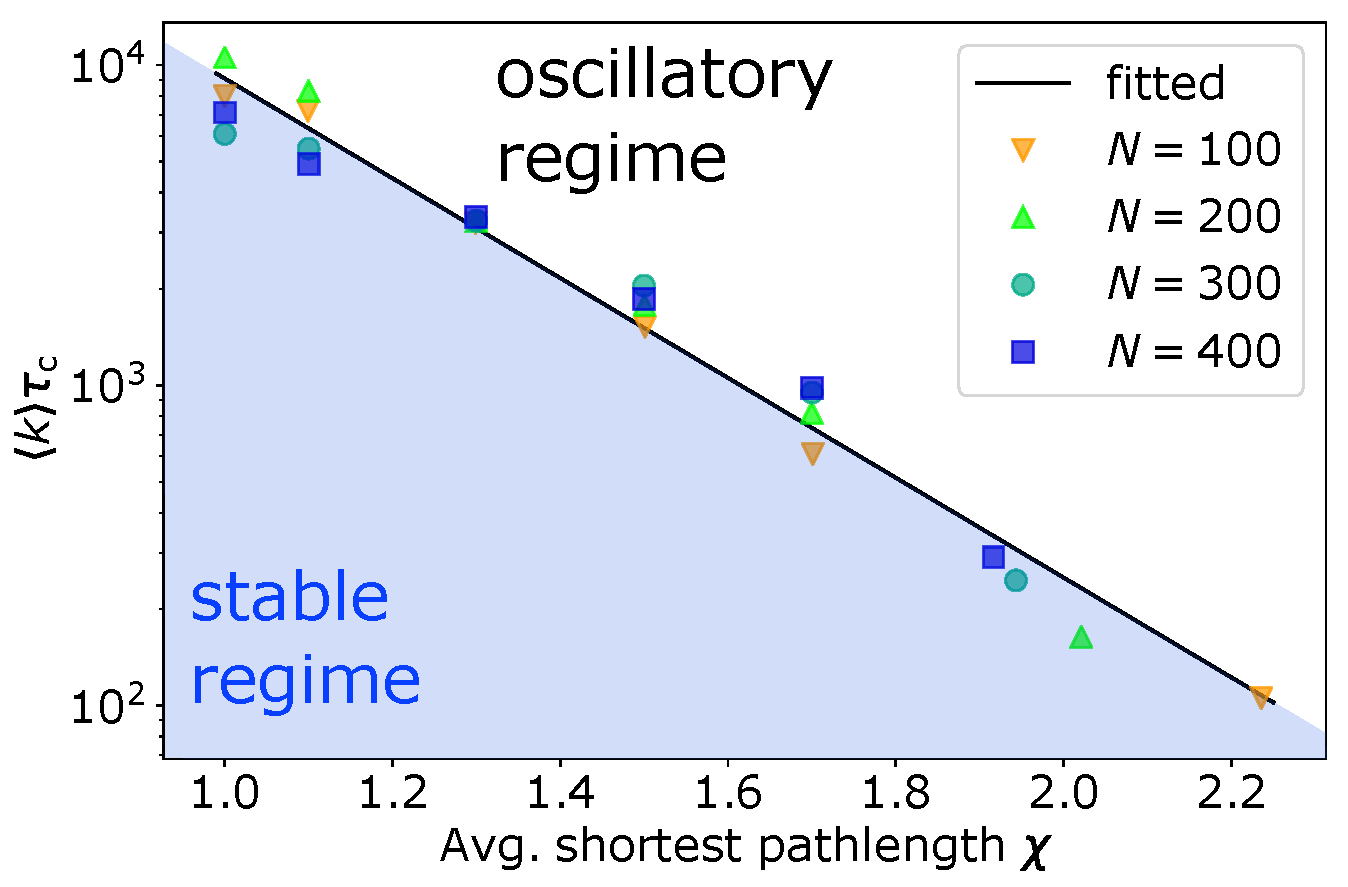
\includegraphics[width=0.8\textwidth]
       {figures/fig4.pdf}
       \caption[Scalling behavior of critical social interaction time]{\textbf{The critical social interaction time depends on network properties.}
	The logarithm of the mean number of neighbors $\langle k \rangle$  times the critical interaction time $\tau_{c}$ is plotted vs. the average shortest path length $\chi$ for various values of $N$ and $p$, confirming eq.~\eqref{scaling_relation}. The stable regime ($\tau \! < \! \tau_{c}$) is shaded in blue. 
   \label{taucrit}}
\end{figure}

\section{Discussion and Conclusion}

The primary purpose of the analysis presented in this chapter was to investigate the possible implications of heterogeneous households individually setting their savings rates according to a simple behavioral heuristic. This analysis makes a somewhat surprising conceptual point by demonstrating how emergent inequality and endogenous dynamics can naturally emerge from a heterogeneous behavioral model. Despite its simplicity, the model accurately predicts that during recessions savings rates increase before output rises (see fig.~\ref{fig:micro_trajs}).
This has been observed for private savings in 19 OECD countries \citep{adema2015business}. 

Household savings rates are influenced by many things, and conspicuous consumption is only one of many factors. Standard macroeconomic models assume that agents are perfect utility maximizers, and attempt to provide realism by imposing frictions that restrict their behavior. Behavioral experiments, in contrast, indicate that real human beings are at best approximate utility maximizers.  Are the behaviorally observed deviations from utility maximization important for macroeconomics?  Can models that explicitly use behavioral rules capture features that standard models miss?

Absent shocks, standard macroeconomic models move toward an equilibrium and remain there.   Dynamics occur only because shocks knock the economy away from equilibrium. In this model, in contrast, the economy may display irregular endogenous oscillations that are reminiscent of business cycles.  
Although the model has the following two random inputs, they are small and very different in character from the shocks that drive the dynamics of standard models. The first random input determines the time at which individual households update their savings rates determined by a Poisson process. The timing of individual updates must be randomized to ensure that the order in which households update their savings rates varies. The second random input is the copying error for the savings rate.  This is small ($1\%$) and its exact value makes little difference to the behavior as long as it is nonzero. In contrast to standard shocks, which affect the economy as a whole, both of these inputs are at the level of individual households, and affect each household differently. For a large number of households the copying errors cancel out but the endogenous dynamics persist nonetheless. Thus while random inputs are necessary in this model, they do not directly drive booms and recessions as the shocks of standard models do. This is why the economic dynamics in this model can indeed be considered endogenous.

To illustrate the conceptual difference between this model and standard macroeconomic models it is useful to draw an analogy to a simple physical system. Consider the problem of pole balancing, in which a man attempts to move his hand to maintain a pole in a vertical position. The position of the man's hand corresponds to the collection of household savings decisions, and the pole/gravity system represents the economy or more precisely, the accumulation of capital in the economy. 
%\begin{figure}
%  \begin{minipage}[c]{0.5\textwidth}
%
%	\caption[]{{ The problem of pole balancing is analogous to the problem of optimizing savings in an otherwise unstable economy.}  A man attempts to maintain a pole in a vertical position.  This is possible if the pole is long enough, but small errors in the control process drive endogenous oscillations in the angle of the pole.}
%   \label{pole_balancing}
%  \end{minipage}
%  \begin{minipage}[c]{0.5\textwidth}
%    \hspace{2 cm}\includegraphics[width=0.3\textwidth]
%       {figures/fig5.jpeg}
%  \end{minipage}\hfill

%\end{figure}
Short poles tip over more quickly than long poles, making it impossible to maintain a vertical position because the pole will tip over before the man can react.  If the pole is long enough, however, the man can move his hand to compensate, and maintain the pole in a roughly vertical position \citep{insperger2017stick}.  There is a sharp critical transition between stability and instability that occurs when the pole is about a meter in length\footnote{This is trivial to confirm empirically -- simply attempt to balance a pole of 60 cm. vs. 130 cm.}.
Nonetheless, even when the pole is rather long, it is not possible to maintain a perfectly vertical position, and the 
pole oscillates substantially.

An argument in the style of a standard macroeconomic model would posit that the man is a perfect pole balancer, and any deviations in the angle must be driven by external shocks, such as sharp gusts of wind, that suddenly cause the pole to deviate from vertical.  Under this view, after each shock the man moves his hand perfectly to make the pole vertical again as fast as possible, but before he can achieve this, another shock strikes it, making the pole oscillate around its vertical position.  For pole balancing it is clear that this explanation is wrong. Instead, theories that assume that oscillations are endogenously caused by imperfect control provide a better explanation for empirically observed behavior \citep{insperger2017stick}.
%Jobst reworded this to save space: provide a good explanation of the empirically observed behavior \cite{insperger2017stick}.  

The suggestion here is that the conceptual explanations for business cycles should be revisited as well.  This model adds weight to the idea that at least part of the variation in savings and investment that occurs during business cycles emerges endogenously due to the imperfect reasoning of households and firms.  The model also suggests that models incorporating agent heterogeneity might help illuminate the interaction between business cycles and inequality.  The fact that such rich behavior emerges from such a simple model supports a research agenda for macroeconomics based on empirically derived behavioral rules.

In the scope of this thesis, this chapter presents a surprisingly rich and interesting answer to a simple curious question. However, from the theoretical perspective, the analysis in this and the previous chapter were rather ad hoc. Although the results were interesting, analytical methods were only used to facilitate more efficient numerical analysis or as --- however well fitting --- still rudimentary approximation of model dynamics. Consequently the insights are limited to the specific cases that were studied. But it is apparent that both models have similarities with respect to the structure of interactions between individual agents. Namely, they both feature interactions between heterogeneous agents both on an individual basis that is structured by some form of network as well as through aggregated variables such as supply and demand.\footnote{This is also the case in many other socio-economic and social-ecological models that describe heterogeneous agents interacting with each other as well as aggregate market interaction, management of public goods of the state of a collectively managed resource.}. Also, in the broader view of describing bounded rational agents in \emph{whole} Earth models I want to better understand models like the ones presented in this and the previous chapter with analytical tools. This raises the question, whether a more general approach for an analytical description of the dynamical properties of these and other similarly structured models is possible. Consequently, in the subsequent chapter I develop an analytical approximation method for such models with networked heterogeneous agents that interact on an individual as well as on a mean field level.

        %% main text
\chapter{Macroscopic Approximation methods for networked agent-based models}
\label{chapter:approximation}
In this chapter, I develop a method to find approximate solutions to heterogeneous-agent models with interactions that happen pairwise as well as on a mean field level. To introduce, I elaborate on the implications that this has for the use of agent-based models in economics in section \ref{sec:approx_intro}. I develop the method at hand of a simplification of the model that I introduced in section \ref{sec:heuristics_model} and will give a short recap of the simplified model specifications in section \ref{sec:approx_Model_Description}. I give a detailed explanation of the method in section \ref{sec:Approximation} and illustrate one of its advantages by doing a bifurcation analysis of the approximated model in section \ref{sec:bifurcation-analysis}. I close this chapter with a conclusion in section \ref{sec:approx_conclusion}


\section{Introduction}
\label{sec:approx_intro}

% Introduction to agent-based models
Agent-based modeling is a computational approach to simulate systems composed of a large number of similar sub-units with many applications in ecology \citep{Grimm2005}, business \citep{Bonabeau2002}, sociology \citep{Macy2002} and economics \citep{Tesfatsion2006, Hamill2015}.
ABMs are used to study aggregate phenomena emerging from local interactions \citep{Epstein1999}.
These interactions can be structured by spatial embedding of agents or by social networks \citep{Gross2008,Holme2006a,Bargigli2014}.

% applications in economics
In economics, ABMs have been used to study for example business cycles \citep{DelliGatti2008}, market power \citep{Tesfatsion2006} and trade \citep{Hamill2015}.

% Introduction to macroeconomic modeling and the aggregation problem
ABMs are a promising alternative to dynamic stochastic general equilibrium (DSGE) modeling, the current workhorse of theoretical macroeconomics \citep{Farmer2009b}. 
DSGE models usually build on the representative agent approach, i.e., they represent all individuals of one type such as firms or consumers by one representative decision maker \citep{Hartley2002}. This is done mainly to hold up to Lucas' influential critique that macroeconomic model should not use statistical correlations between aggregate variables but rather build on the behavior of individual economic agents \citep{Janssen2016, Lucas1976}.

% Disadvantages/critique of representative agent, 
% pros and cons of DSGEs
% cons:
The representative-agent approach implies that theoretical macroeconomics reduces macroeconomic phenomena to assumptions about a few different representative agents, leaving out many explanatory mechanisms for fluctuations in aggregate variables based on intra-group interaction and heterogeneity.\footnote{Approaches to represent heterogeneous agents in DSGE models have been used to counter this criticism and add more realism regarding the distribution of agent attributes \citep[see for example the review by][]{Heathcote2009}.
Particularly, because the representative agent approach cannot account for interactions within a heterogeneous group, models using this approach do not allow for the representation of emergent phenomena \citep{Kirman1992}\footnote{Here, we use a weak notion of emergence, which allows explaining macro-phenomena on the basis of micro-interactions of the systems constituents that differ from the explained macro-phenomena. This is opposed to strong emergence, that embraces the irreducibility of macro-phenomena to lower-level dynamics. For a discussion see \citet{Bedau1997}.}
but their solution requires complex numerical methods and cannot integrate local interactions between agents.}
Furthermore, DSGE model often assume rational expectations, i.e., agents know the constraints and dynamics of the entire economy. This has been criticised as philosophically unsound and empirically unjustified \citep{Kirman2014}.
% pros:
However, due to these assumptions, most DSGEs allow for a thorough analytical analysis.

% pros and cons of ABMs:
% pros:
In contrast, ABMs allow implementing various individual decision models that are behaviorally more realistic than full economic rationality  \citep{Mueller-Hansen2017}.
Agents are often assumed to be boundedly rational and adapt their expectations, which is compatible with the Lucas critique \citep{Evans2006}.
In ABMs, fluctuations in aggregate variables do not only arise from exogenous shocks as in DSGE models but primarily from irregularities in local interactions \citep{Tesfatsion2001}.
Therefore, they offer an avenue for explaining various emergent phenomena studied in empirical macroeconomics \citep{Tesfatsion2006a}.

% cons:
As a potential downside, ABMs are often very detailed so that an analytic treatment is unfeasible. 
Therefore, in ABMs, the difficulties arising from the aggregation of heterogeneous and interacting agents are usually solved computationally.
Because the model mechanisms are difficult to trace in the `black box' of a computational model, the results of ABMs are often difficult to interpret and cannot provide mathematically sound proofs of relationships between model variables. Results may therefore be difficult to generalize \citep{Leombruni2005}.
There has been some progress in the standardization of model descriptions for ABMs \citep{Grimm2006}, but the lack of standardization, e.g., of decision rules, makes the models difficult to compare \citep[][p. 239]{Hamill2015}. Even though there are various techniques available for comprehensive model analysis \citep{Lee2015}, a systematic model exploration is uncommon and mostly limited to sensitivity analysis with respect to crucial parameters.

% Bringing the two together
Methods from theoretical physics have been applied successfully to various problems in economics for many years \citep{Mantegna1999}. Here, aggregation methods from statistical physics can bridge the gap between analytic macroeconomic models such as DSGE approaches and agent-based computational models \citep[for a review of physics methods in social modeling, see ref.][]{castellano2009statistical}. In contrast to macroeconomic models, these approaches account for local interactions and use aggregation techniques to derive macro-dynamics, providing a true microfoundation of the resulting macromodel.
These kinds of approximation methods have recently found much interest in the fields of financial economics \citep{DiGuilmi2008, DiGuilmi2012a, Chiarella2011a} and behavioral finance \citep{Hommes2017BoomsPrices} and have produced interesting and promising results, e.g., to explain macroeconomic fluctuations and understand propagation of financial shocks and the resulting systemic risk.

%short discussion of some of the work already done in this field

% include this literature as well?
%Di Guilmi et al. 2012 (SSRN): Credit network economy, analytical approximation via Master equation
%Delli Gatti et al. 2005 (JEDC): interacting agents, mention of network but use unclear
%Gualdi et al. 2015 (JEDC): Analysis of Delli Gatti model (see books) in phase space, identification of tipping behavior
% \citep{DelliGatti2008}: stochastic aggregation very general and not related to networks

Many authors use mean field approximations to study interactions between heterogeneous agents, e.g., making use of Master and Fokker-Planck equations \citep{Aoki1998, Aoki2007, DelliGatti2000, DiGuilmi2008, Chiarella2011a, Landini2014}. Such approaches assume that each agent pair interacts with the same probability.
But many social and economic interactions are structured and the structure can be described by complex networks \citep{Friedkin2011}. Therefore, some approximation methods take network structure into account and derive macroscopic quantities that describe the structure of networks \citep[e.g.][]{Alfarano2008a, Lux2016}.

Yet, most of the literature regards either the network between agents or the states of agents as static, implicitly assuming different time scales for dynamics of and processes on the network.
However, recent literature on opinion formation processes and the spreading of social norms in the field of computational social sciences suggests that both happen on a comparable timescale and can therefore not be treated separately \citep{Gross2008, gross2009adaptive}.
A typical example of a model that takes this into account is the one that I present here. I use this model to demonstrate how the individual techniques mentioned above may be combined. In this model, the network of interactions between agents as well as the spreading of behavior between agents on this interaction network happen on a comparable timescale.
For such adaptive networks \citep{Gross2008}, moment closure techniques have been introduced in the physics literature to aggregate the feedback between complex adaptive network dynamics and dynamics of single node states \citep{Do2009, Demirel2014, Wiedermann2015, Min2017}.
Here, I introduce these techniques to economic modeling and combine them with approaches from macroeconomics where interactions also happen globally via aggregated variables.

% Discussion of usefulness of analytic approximations
The technical challenges of analytic approximation methods for agent-based model has so far hampered their wide-spread use in economics. But they have a huge potential in providing profound insights into dynamical properties of economic systems: First, they help increasing performance of computer simulations, making calculation of single model runs much faster and therefore allowing for a wider range of bifurcation and parameter analyses. Second, in contrast to stochastic simulations, they make formal proofs of relations between macroscopic variables possible. Third, they allow the derivation of analytical expressions of relations between model variables from the dynamic equations, which is not possible from single simulation runs. This work makes a step forward in showcasing how such methods can be used to combine interactions on complex adaptive networks with macroeconomic modeling. It is therefore a contribution to integrate non-standard behavioral assumptions into macroeconomic models.

% Contribution of this paper % Introduce the model in the paper
This chapter relies on a simplification of the ABM that was introduced in section \ref{sec:heuristics_model}. The model consists of heterogeneous households that interact and learn from neighbors on a social network and a two-sector productive economy.
Agents imitate the investment strategy of acquaintances that are better off with a higher probability.
This model is used to show how these approximation techniques can be applied to models that combine local interactions on a network with system-level interactions through markets.
In particular, I use a combination of moment closure, pair, and large system limit approximations to derive an aggregate description for the dynamics of my model. Moment closure is used to describe the properties of heterogeneous households via the moments of their distribution. The pair approximation is used to describe the adaptive network dynamic of the full model by an approximate proxy process, a so called Pair Based Proxy, in terms of aggregate network properties. Both techniques together facilitate a low dimensional stochastic approximation of the originally very high dimensional ABM. The large system limit is then used to further approximate this proxy process by a set of ordinary differential equations.
To the best of my knowledge this is the first study that applies such a combination of approximation methods on a model that combines structured local with global interactions of heterogeneous agents in a socioeconomic setting.
Self-evidently, despite the fact that the reference application is an economic one, this approximation method can also be used to describe similarly structured models in other fields of research such as social-ecology, neuroscience or computational social science.

% Outline
In the following section, I give a specification of the model that I use to illustrate the approximation method. As the model is a simplification of the one introduced in section \ref{sec:heuristics_model}, I will not discuss its details again but only give a short recap of its specifications and elaborate on the simplifications.
%In the remainder of the paper, I first describe the details of the model (Sec.~\ref{sec:approx_Model_Description}). Then, I derive an aggregate description of the model by applying three approximation techniques, moment closure, pair approximation, and large system limit (Sec.~\ref{sec:Approximation}). I discuss commonalities and differences between computer simulations and the approximation approach. Before concluding, I illustrate how the derived macro-approximation can be used in a bifurcation analysis to better understand the qualitative properties of the non-linear model (Sec.~\ref{sec:bifurcation-analysis}).

\section{Model Description}
\label{sec:approx_Model_Description}

To illustrate the application of the methods that I put forward, I use a model of a stylized two sector investment economy that captures the shift from fossil-fuel to renewable energy-based based production. Essentially, this equals the model that I introduced in section \ref{sec:heuristics_model} with the difference that I abstract from the separation of judgement and actions in terms of a heuristic decision model. Instead, households decisions whether to invest in one or the other sector are directly governed by the adaptive voter dynamic \citep{Holme2006a}.
Consequently, if the reader still has the model in mind, they can safely skip the model description and continue with section \ref{sec:numerical_results} where I present first results.

This model is designed to incorporate the dynamics of social norms that underlie investment decisions in the context of climate economics and policy. Decarbonization pathways consistent with the Paris agreement require a rapid shift of investments away from fossil fuel exploration and extraction to the development and deployment of renewable energies \citep{IPCC2014}. However, the implementation of climate policies is uncertain and expectations cannot be based on self-consistent beliefs about the future.  In conventional macroeconomic models such shifts can only occur due to price signals either from improvements in renewable technology, increasing scarcity of fossil reserves, or carbon pricing. While price signals are certainly important, movements advocating for the divestment from fossil fuels point to the role of social norms and practices regarding investment decision to initiate and accelerate the energy transition \citep{Ans2013,Nyborg2016}. To better understand such culturally driven situations of socioeconomic change, it is important to work with models that can incorporate endogenous preferences and aspects of bounded rationality such as imperfect foresight and information as well as learning.
%\begin{figure}[t]
%  \centering
%  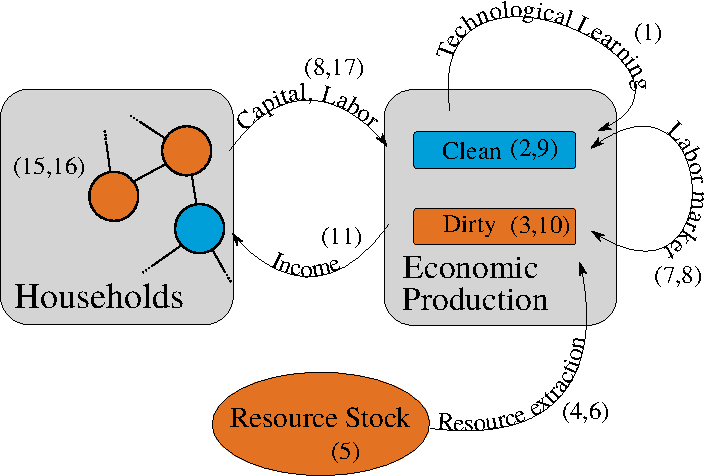
\includegraphics[width=.8 \textwidth]{figures/model_scheme.pdf}
%\caption{Schematic figure of the model consisting of two production sectors of which one depends on an exhaustible fossil resource stock as well as a set of heterogeneous households that interact on an adaptive complex network and use social learning to decide upon which of two production sectors to invest in. Boxes and bubbles denote modeled entities, arrows denote interactions. Numbers in brackets $(x)$ refer to equations $(6.x)$ that describe the specific part of the model.}
%  \label{fig:model_scheme}
%\end{figure}
% \subsection{Economic Production}
\label{sec:approx_economy}

The underlying assumptions of the economic model are discussed in detail in section \ref{sec:heuristics_model}. This is a brief recap of the specifications of the economic production model. 

The model consists of two sectors for production and a set of heterogeneous households that interact via a complex adaptive social network. The two production sectors employ different technologies where the production technology in one sector depends on the input of an exhaustible (fossil) energy-resource $R$ that is used up in the economic production process whereas the technology in the other sector does not. They are called the \textit{dirty} and the \textit{clean} sector accordingly. Capital is technology specific and can not be reallocated between the two sectors.
Therefore, the heterogeneous households in the model provide different types of capital $K_j$ as well as labor $L$ to the sectors.
The technology in the dirty sector is fully developed and adequately described in terms of the total factor productivity. 

The clean sector represents a circular economy\footnote{A circular economy is an economic system that employs sharing, reuse, repair, refurbishment and recycling to create a close-loop system that minimizes the use of resource inputs and waste outputs, pollution and carbon emissions \citep{Stahel2016, Geissdoerfer2017}.} in which the output of final goods depends on the machinery, knowledge and effort used in its production and is not limited by entropy laws\footnote{It is often noted, that circular economic processes are eventually limited by the second law of thermodynamics, stating that even though the material flows in economic activity may be circular, they still produce excess entropy that on would have to get rid of. Consequently, in this scheme, economic growth is eventually limited by the earths capacity to get rid of entropy in the form of high entropy radiation \citep{Georgescu-Roegen1993, Kaberger2001, Korhonen2018}.} or resource scarcity on the timescale under consideration. The technology $C$ used in the clean sector is assumed to be still in development and is therefore explicitly modeled.
Technological progress is implemented as learning by doing according to Wright's law \citep{wright1936factors, Nagy2013} with a one-factor learning curve. $C$ is proportional to the cumulative production $\int Y_c \mathrm{d}t$ but also depreciates with a constant rate $\chi$.

\begin{equation}
	\dot{C} = Y_c - \chi C.
	\label{eq:approx_lbd}
\end{equation}

Capital, labor and technology/knowledge are mutual substitutes. The production functions $Y_c = b_c C^{\gamma} L_c^{\alpha_c}K_c^{\beta_c}$  for the clean and 	$Y_d = \mathrm{ min}\left( b_d L_d^{\alpha_d}K_d^{\beta_d}, e R \right),$ for the dirty sector satisfy these requirements. Subscripts $c$ and $d$ denote the clean and dirty sector respectively, $L_c$ and $L_d$ are labor shares, $\alpha$ and $\beta$ are elasticities of the respective input factors, $b_c$ and $b_d$ are the total factor productivity and $K_c$ and $K_d$ are the capital stocks for the respective sector.
The dirty sector uses the resource efficiently, such that
\begin{equation}
    b_d L_d^{\alpha_d}K_d^{\beta_d} = e R
    \label{eq:approx_edr}
\end{equation}
where $1/e$ is the resource intensity of the sector. The usage of the fossil resource $R$ depletes a geological resource stock $G$ with the initial stock $G(t=0) = G_0$:
\begin{equation}
    \dot{G} = -R. 
    \label{eq:approx_rdep}
\end{equation} 
The total cost $c_R$ for the usage of the fossil resource depends on the resource use $R$ and the remaining fossil resource stock $G$ as $c_R = b_R R^{\rho}\left( \frac{G_0}{G} \right)^{\mu}$ with $\rho \geq 1$ and $\mu > 0$ such that $\partial c_R / \partial R >0$ and $\partial c_R / \partial G < 0$.
This means that at some point $\partial Y_d / \partial R < \partial c_R / \partial R$ to take into account that some part of the resource is not economic as its marginal cost exceeds its marginal productivity.
The equilibrium wage $w$ equals the marginal return for labor:
\begin{equation}
	w = \frac{\partial Y_c}{\partial L_c} = \frac{\partial Y_d}{\partial L_d} - \frac{\partial c_R}{\partial L_d}
	\label{eq:approx_equilibrium_wage}
\end{equation}
with the sum of the labor shares equal to the total amount of labor available:
\begin{equation}
	L_c + L_d = L.
	\label{eq:approx_L}
\end{equation}
Capital rents equal marginal productivity i.e., 
\begin{align}
  r_c &= \frac{\partial Y_c}{\partial K_c}, \label{eq:approx_ccr}\\
  r_d &= \frac{\partial Y_d}{\partial K_d} - \frac{\partial c_R}{\partial K_d}. \label{eq:approx_dcr}
\end{align}

\subsection{Adaptive Network Model for Investment Decision Making}
\label{sec:investment_decision_making_descr.}
%\JJK{Maybe comment on the relationship between individual optimization, group level optimization and the imitation of successful strategies.}
For the approximation methods derived here, I have to abstract from the separation of judgment and actions that I proposed in section \ref{sec:intro_learning_heuristics} and \ref{sec:investment_decision_making}.
Still, I model households as bounded rational decision makers \citep{simon1972theories, simon1982models, gigerenzer2002bounded}.
That is, households take their investment decisions, i.e. whether to invest their savings in the clean or the dirty sector, not by forming rational expectations \citep{Evans2006, Kirman2014} but by engaging in social learning \citep{Bandura1971} to obtain successful strategies \citep{Traulsen2010} with reasonable effort.
As the outcomes of social learning crucially depend on the structural properties of the complex network of social ties amongst the households \citep{Barkoczi2016}, I model the adaptive formation of this social network endogenously.
A well established principle for the emergence of structured ties in social networks is homophily, i.e. the tendency that similar individuals are linked \citep{McPherson2007, Centola2007, Centola2011}.
The following model specification uses social learning in combination with endogenous network formation based on homophily to model the investment decisions of the households.

I model $N$ heterogeneous households denoted with the index $i$ as owners of labor $L^{(i)} = L/N$ and capital $K_c^{(i)}$ and $K_d^{(i)}$ in the clean and dirty economic sector respectively.
Households generate an income $I^{(i)}$ from their labor and capital income which they use for consumption $F^{(i)}$ and savings $I^{(i)}$:
\begin{align} 
	I^{(i)} &= w L^{(i)} + r_c K_c^{(i)} + r_d K_d^{(i)}, \label{eq:approx_hi} \\
	F^{(i)} &= (1-s) I^{(i)}, \label{eq:approx_c} \\
	S^{(i)} &= s I^{(i)}. \label{eq:approx_s}
\end{align}
where $s$ is the savings rate that specifies the fraction of income $S^{(i)}$ that saved and $r_c$ and $r_d$ are the rents for clean and dirty capital respectively.
A binary decision parameter $o_i \in \{c,d\}$ denotes the sector in which the households decide to invest. Investment decisions are driven by social learning via the imitation of successful strategies and homophily towards individuals exhibiting the same behavior. \\
I describe households as the nodes in a graph of acquaintance relations that follow the following rules: 
\begin{enumerate}
    \item Households randomly become active at a constant rate $1/\tau$ i.e. their activity is given by a Poisson-Process. \label{r1}
        \item When a household $i$ becomes active, it interacts with one of its acquaintances $j$ chosen uniformly at random. 
        \item If they follow the same strategy, i.e. they invest in the same sector, nothing happens. 
        \item If they follow a different strategy, i.e. they invest in different sectors, one of two actions can happen:
        \begin{enumerate}
                \item Homophilic network adaptation: with probability $\varphi$, the households end their relation and household $i$ connects to another household $k$, that follows the same strategy. 
                \item Learning: with probability $1-\varphi$, household $i$ engages in social learning i.e. it imitates the strategy of household $j$ with a probability $p_{ji}$ that increases with their difference in income. \label{rn}
        \end{enumerate}
\end{enumerate}
I follow previous results on human strategy updating in repeated interactions from \cite{Traulsen2010}, when I assume the imitation probability as a monotonously increasing function of the relative difference in consumption between both households:
\begin{equation}
	p_{ji} =  \left(1 + \exp \left(- \frac{a(F^{(i)} - F^{(j)})}{F^{(i)} + F^{(j)}} \right) \right)^{-1}.
    \label{eq:approx_ip}
\end{equation}
As opposed to the absolute difference in the original study by \cite{Traulsen2010}, the probability in this model depends on relative differences. 
I set $a = 8$ to conform to their empirical evidence. This dependence on relative differences in per household quantities is crucial for my method as I will discuss later at the end of section \ref{sec:large_system_limit}.
I model strategy exploration as a fraction $\varepsilon$ of events that are random, e.g. rewiring to a random other household or randomly investing in one of the two sectors.
Given the savings decisions of the individual households, and assuming equal capital depreciation rates $\kappa$ in both sectors, the time development of their capital holdings is given by

\begin{align}
	\dot{K}_c^{(i)} =& \delta_{o_ic} \left( r_c K_c^{(i)} + r_d K_d^{(i)} + w L_i \right) - \kappa K_c^{(i)} \label{eq:approx_ci}\\
	\dot{K}_d^{(i)} =& \delta_{o_id} \left( r_c K_c^{(i)} + r_d K_d^{(i)} + w L_i \right) - \kappa K_d^{(i)} \label{eq:approx_di}
\end{align}

where $\delta_{ij}$ is the Kronecker Delta. The total capital stocks in the two sectors are made up of the sum of the individual capital stocks as
\begin{equation}
    K_j = \sum_i^N K_j^{(i)} = N k_j, \qquad j \in \left\{ c, d \right\}
\end{equation}
where $k_j$ is the average per household capital stock of a given capital type.

I acknowledge the fact that different model specifications are possible and interesting.
For instance, I only consider fixed savings rates and the decision between two capital assets and leave the analysis of the interesting possible effects of households setting their savings rates individually to another study \citep{Asano2019}.
However, I want to point out that the approximation methods that I develop in the following can also be useful to gain insights from different but similar models that rely on complex adaptive interaction networks.


   
\subsection{Numerical Modelling and Results} 
\label{sec:numerical_results}
\textcolor{red}{I think that this subsection is a candidate for removal.}\\

% JK: distinguish better between assumptions, initial conditions and findings/results.
With the model specifications from section \ref{sec:approx_Model_Description}, the parametrization in Tab.~\ref{tab:Parameter_list} and appropriate initial conditions for the dynamic variables, the model can be simulated numerically.
For this, I implemented the dynamics in the multi-purpose programming language python. The implementation of the ABM as well as the numerical analysis using the approximation methods described in the following are available on github in \cite{kolb2018}.
In the following, I discuss the resulting aggregate dynamics.

\begin{figure}[ht]
  \centering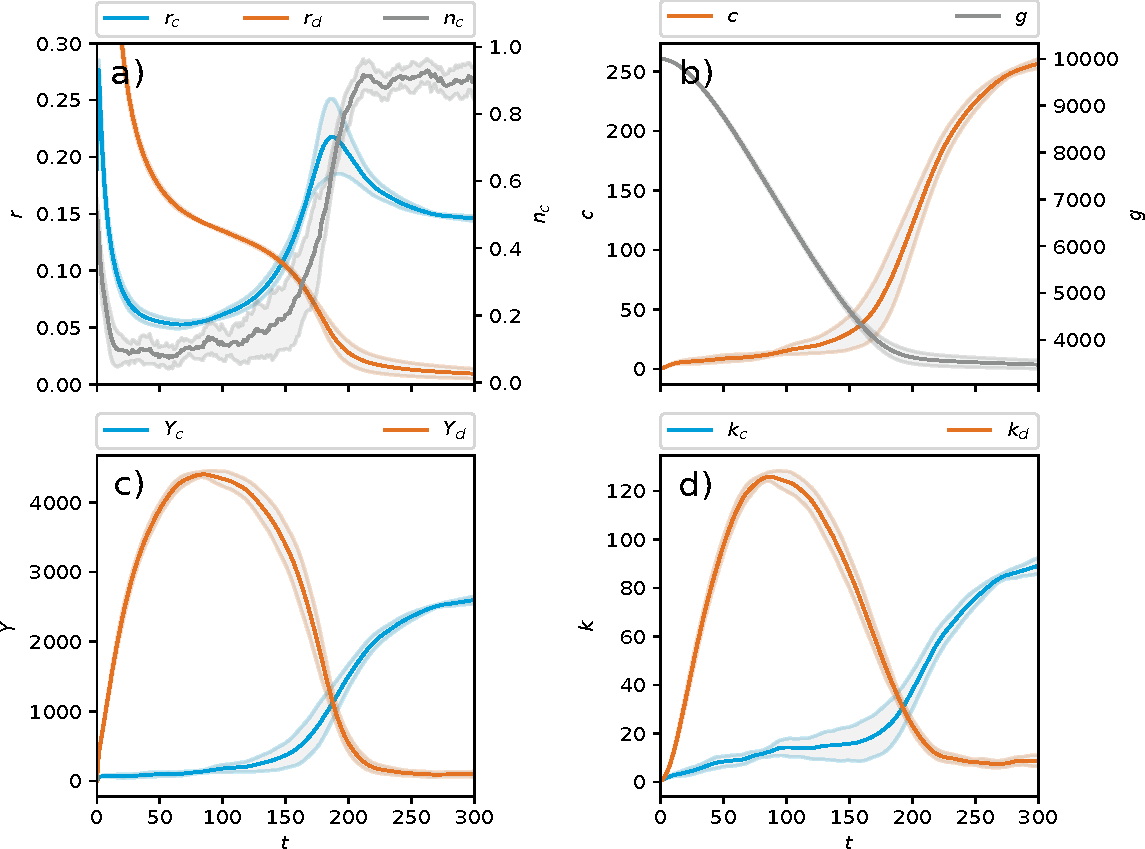
\includegraphics[width=.85\linewidth]{figures/example_trajectory.pdf}
  \caption{\textbf{Example trajectory of the ABM.} Solid lines show mean results from 100 runs of the model in per capita variables. Grey areas around solid lines show their standard deviation. The panels show capital rents in the clean and dirty sector $r_c$ and $r_d$ as well as the fraction of households investing in the clean sector $n_c$ in panel a, knowledge and resource stock $c$ and $g$ in panel b, output of clean and dirty sector $Y_c$ and $Y_d$ in panel c and per capita capital $k_c$ and $k_d$ in the clean and dirty sector (d).
Initial conditions are $G=G_0$, $C=1$, $K_j^{(i)}=1$ for the economic subsystem. For the investment decision process, the initial opinions of the $N=100$ households are drawn from a uniform distribution. Their initial acquaintance structure is an Erd\H{o}s-Renyi random graph with mean degree k=10.}
\label{fig:example_trajectory}
\end{figure}

Figure \ref{fig:example_trajectory} displays an exemplary average evolution of the model calculated as the mean of 100 simulation runs.
The simulation starts with initial conditions of abundant fossil resources $g$ and low clean technology knowledge stock $c$ (panel b) as well as equally low capital stocks in the clean and dirty sector $k_c$ and $k_d$ (panel d). As I show later (see section~\ref{sec:bifurcation-analysis}), the rest of the initial configuration of the model is rather irrelevant for the selected parameter values listed in Tab.~\ref{tab:Parameter_list}, since there is only one stable dynamical equilibrium as long as resource extraction costs are negligibly low.
The high initial capital rents $r_c$ and $r_d$ are a direct result of the model assumptions and initial conditions. More precisely, the assumption that capital rent equals marginal productivity in eq. \ref{eq:approx_ccr} and \ref{eq:approx_dcr} and that of decreasing marginal productivity due to the choice of $\beta_i$ in combination with the initial condition of low capital and a fixed labor supply. Also as a direct consequence of these assumptions, the capital rents $r_c$ and $r_d$ decrease over time as the capital stock is built up.
Initially (from $t=0$ to $t=100$), as a result of the choice of total factor productivities $b_i$ and due to low fossil resource extraction costs, capital productivity (and therefore capital rent $r$) is higher in the dirty sector than the clean sector (see panel a). 
Consequently, the majority of households invest in the dirty sector which leads to a high per-household capital stock $k_d$ (panel d) and high production output $Y_d$ (panel c) in this sector.

Regarding the capital rents, I would expect the system to move towards a dynamic equilibrium in which the capital rent is equal in both sectors, i.e., $r_d = r_c$, if everything else remained constant. However, I find that there is a persisting difference between $r_c$ and $r_d$ between $t=50$ and $t=100$.
This difference can be explained by the exploration of investment strategies, which brings the shares of clean and dirty investors closer together. In terms of the depicted variables this means that it brings $n_c$ closer to $0.5$. 
% \FMH{I reformulated the last sentences, because they were difficult to understand, please check! - Checked}

For $t>100$ the depletion of the fossil resource leads to significantly increasing resource extraction costs. Consequently, the marginal productivity of dirty capital $k_d$ decreases and so does $r_d$, leading to a peak in accumulation of capital in the dirty sector around $t=100$ (panel d).
Once the relative return on capital in the clean sector increases, households start to adopt a clean investment strategy visible in an increase in $n_c$ in panel a.
When the fossil resource stock reaches its economically exploitable share at around $t=200$, the overall productivity in the dirty sector reaches zero, leading to full employment of all available labor in the clean sector.
This drives demand for capital up, accelerating the investment change from clean to dirty investment.
As all households except for the share caused by exploration are investing in the clean sector, the system reaches an equilibrium with high capital in the clean sector and low capital in the dirty sector.

Notably, I find an increasing variance in the fraction of households investing in the clean sector before and around the transition, which means that due to the stochasticity of the social learning process the transition happens earlier for some simulation runs than for others. Nevertheless, I find that the inertia of the model resulting from the large accumulated stock of capital that is specific to the dirty sector eventually leads to an almost entire depletion of the fossil resource.

\begin{table}
	\centering
	\begin{tabular}{l|l|l}
		\hline
		$b_c$ & 1. & Total factor productivity in the clean sector \\
		$b_d$ & 4. & Total factor productivity in the dirty sector \\
		$b_R$ & .1 & Initial resource extraction cost \\
		$e$   & 1 & Resource conversion efficiency \\
		$\kappa$   & 0.06 & Capital depreciation rate \\
		$\chi$      & 0.1 & Knowledge depreciation rate \\
		$\gamma$	   & 0.1 & Elasticity of knowledge in the clean sector \\
		$\alpha_c$ & 0.5 & Elasticity of labor in the clean sector \\
		$\alpha_d$ & 0.5 & Elasticity of labor in the dirty sector \\
		$\beta_c$ & 0.5 & Elasticity of capital in the clean sector \\
		$\beta_d$ & 0.5 & Elasticity of capital in the dirty sector \\
		$\varphi$ & 0.5 & Fraction of rewiring events in opinion formation \\
		$1/\tau$ & 1. & Rate of opinion formation events \\ 
		$\varepsilon$ & 0.05 & Fraction of noise events in opinion formation \\ 
        $G_0$ & 1000000 & Initial resource stock \\
        $L$ & 100 & Total labor \\ 
        \hline
	\end{tabular}
	\caption{List of model parameters with their default values}
	\label{tab:Parameter_list}
\end{table}

\section{Approximate Analytical Solution}
\label{sec:Approximation}

Structurally, the model described in section \ref{sec:approx_Model_Description} consists of a set of coupled ordinary differential equations \cref{eq:approx_lbd,eq:approx_rdep,eq:approx_ci,eq:approx_di} with algebraic constraints \cref{eq:approx_edr,eq:approx_equilibrium_wage,eq:approx_L,eq:approx_ccr,eq:approx_dcr} for the economic production process and a stochastic adaptive network process for the social learning component that is described by the rules \ref{r1} to \ref{rn} in section \ref{sec:investment_decision_making_descr.}. The state space of this combined process consists of two degrees of freedom of the knowledge stock and the geological resource stock as well as $2N$ degrees of freedom for the capital holdings of the set of all individual households plus the configuration space of the adaptive network process of the social learning component. I denote the variables of this process by capital letters ($C, G, K_j^{(i)}\dots$).
To find an analytic description of the model in terms of a low dimensional system of ordinary differential equations, I approximate it via a Pair Based Proxy (PBP) process, a stochastic process in terms of aggregated quantities, thereby drastically reducing the dimensionality of the phase space. I denote the variables of this process with capital letter with bars ($\bar{X}, \bar{Y}, \bar{Z}, \bar{K}_l^{(k)}\dots$).

The derivation of this approximate process is done in three steps: First, I solve the algebraic constraints to the economic production process given by market clearing in the labor market and efficient production in the dirty sector - loosely following \cite{Nitzbon2017}. Second I use a pair approximation to describe the complex adaptive network process of social learning in terms of aggregated variables, similar to \cite{Rogers2012}. Third, I use a moment closure-like method to approximate higher moments of the distribution of the capital holdings of the heterogeneous households by quantities related to the first moments of their distribution.

Finally, I take the limit of infinitely many households (large system- or thermodynamic limit) to obtain a deterministic description of the system.

\subsection{Algebraic Constraints}
%\JJK{Most of this subsection could move to supplementary material to be replaced by a verbal explanation, depending on the journal requirements}

To calculate the labor shares $L_c$ and $L_d$ as well as the wages in the two sectors, one uses equations \eqref{eq:approx_equilibrium_wage} and \eqref{eq:approx_L} and for simplicity assumes $\rho=1$ and $\mu=2$. Additionally, one assumes equal labor elasticities in both sectors $\alpha_d = \alpha_c = \alpha$. A series of algebraic manipulations that was done before in section \ref{sec:algebraic_constraints} solves the algebraic constraints to the ordinary differential equations describing the economic production and eventually leads us the set of independent equations below:

\begin{subequations}
\begin{empheq}{gather}
	X_c = (b_c K_c^{\beta_c}C^{\gamma})^{\frac{1}{1-\alpha}}, \quad X_d = (b_d K_d^{\beta_d})^{\frac{1}{1-\alpha}}, \quad X_R = \left( 1 - \frac{b_R}{e}\frac{G_0^2}{G^2} \right)^{\frac{1}{1-\alpha}}, \\
	w = \alpha L^{\alpha-1}\left( X_c + X_d X_R \right)^{1-\alpha}, \label{eq:approx_equilibrium_wage_solution}\\
	r_c = \frac{\beta_c}{K_c}X_c L^{\alpha}\left( X_c + X_d X_R \right)^{-\alpha}, \\
	r_d = \frac{\beta_d}{K_d}X_d X_R L^{\alpha}\left( X_c + X_d X_R \right)^{-\alpha}, \\
	R = \frac{b_d}{e}K_d^{\beta_d}L^{\alpha}\left( \frac{X_d X_R}{X_c + X_d X_R} \right)^{\alpha}, \\
	\dot{G} = - R \label{eq:approx_surd}, \\ 
	\dot{K}_c^{(i)} = s \delta(o_i - c) (r_c K_c^{(i)} + r_d K_d^{(i)} + w L^{(i)}) - \kappa K_c^{(i)}, \label{eq:sum_up_clean_capital_accumulation} \\
	\dot{K}_d^{(i)} = s \delta(o_i - d) (r_c K_c^{(i)} + r_d K_d^{(i)} + w L^{(i)}) - \kappa K_d^{(i)}, \label{eq:sum_up_dirty_capital_accumulation} \\
        \dot{C} = Y_c- \chi C.\label{eq:sum_up_learning}
\end{empheq}
\end{subequations}

\subsection{Pair Approximation}
\label{sec:pair_approximation}
To derive a macroscopic approximation of the social learning process described by rules \ref{r1} to \ref{rn} in section \ref{sec:investment_decision_making_descr.}, I make use of a Pair based proxy (PBP) process that is derived via pair approximation from the adaptive network process. This proxy process is not equivalent but sufficiently close to the microscopic process approximating it in terms of aggregated quantities by making certain assumptions about the properties of their microscopic structure. The aggregated quantities of interest are: the number of households investing in clean capital $N^{(c)}$, the number of households investing in dirty capital $N^{(d)}$, the number of links between agents of the same group $[cc]$ and $[dd]$ as well as between the two groups $[cd]$. Since the total number of households $N$ and links $M$ are fixed, these five variables reduce to three degrees of freedom, which I parameterize as follows:

\begin{equation}
	\bar{X} = N^{(c)} - N^{(d)}, \quad \bar{Y} = [cc] - [dd], \quad \bar{Z} = [cd].
	\label{eq:opinion_formation_macro_variables}
\end{equation}

These three degrees of freedom span the reduced state space of the social process $\mathbf{\bar{S}} = (\bar{X}, \bar{Y}, \bar{Z})^T$. The investment decision making process can then be described in terms of jump lengths $\Delta \mathbf{\bar{S}}_j$ and jump rates $W(\mathbf{\bar{S}},\mathbf{\bar{S}} + \Delta \mathbf{\bar{S}}_j)$ in this state space for the different events $j$ in the set $\Omega$ of all possible events.
Their derivation is illustrated by the example of a clean household imitating a dirty household: The approximate rate of this event is given by
\begin{equation}
	W_{c \rightarrow d} = \frac{N}{\tau} (1-\varepsilon) (1 - \varphi) \frac{N^{(c)}}{N}\frac{[cd]}{[cd] + 2 [cc]}p_{cd}.
	\label{eq:cdswitchingprob}
\end{equation}
In some more detail this results from
\begin{itemize}
	\item $N/\tau$ the rate of social update events i.e. the rate of events per household times the number of households,
	\item $(1-\varepsilon)$ the probability of the event not being a noise event,
	\item $(1-\varphi)$ the probability of imitation events (versus network adaptation events),
	\item $N^{(c)}/N$ the probability of the active households to invest in clean capital,
	\item $[cd]/(2[cc] + [cd])$ the approximate probability of interaction with a household investing in dirty capital. Here, I approximate the distribution of dirty neighbors among clean households with its first moment i.e. I act as if links between clean and dirty households were evenly distributed among all households. 
	\item $p_{cd}$ is the expected value of the probability of the active households imitating its neighbor depending on the difference in consumption between households investing in clean and dirty capital as given in equation \eqref{eq:approx_ip}. The expression is derived in detail as part of the moment closure in subsection \ref{moment_closure}.
\end{itemize}
The corresponding change in the state space variables is a little more tricky. Since the event is a clean household imitating a dirty household, I already know about one of the neighbors of the household. Then the state of the remaining neighbors is approximated by drawing $k^{c} - 1$ times from the distribution of neighbors that is, as before, approximated by an even distribution of edges between same and different households among all households again approximating the respective full distributions with their first moments. Thus the probability for a neighbor to be dirty $p^{(d)}$ or clean $p^{(c)}$ reads:
\begin{equation}
	p^{(c)} = \frac{2 [cc]}{2[cc] + [cd]}; \qquad p^{(d)} = \frac{[cd]}{2[cc] + [cd]}.
\label{eq:neighbordist}
\end{equation}


This results in $n^{(c)}$ additional clean neighbors and $n^{(d)}$ additional dirty neighbors:
\begin{equation}
	n^{(c)} = (1-1/k^{(c)})\frac{2[cc]}{N^{(c)}}, \quad n^{(d)} = (1-1/k^{(c)})\frac{[cd]}{N^{(c)}},
	\label{eq:additional_neighbors}
\end{equation}
where $k^{(c)}$ is the mean degree, i.e. the mean number of neighbors of a clean household in the network.
With the results from \eqref{eq:additional_neighbors} the changes in the expected values of the state space variables can be approximated as follows:
\begin{align}
	\Delta N^{(c)} &= -1 \nonumber \\
	\Delta N^{(d)} &= 1 \nonumber \\
	\Delta [cc] & \approx \left( 1 - \frac{1}{k^{(c)}} \right)\frac{2[cc]}{N^{(c)}} \nonumber \\
	\Delta [dd] & \approx \left( 1 - \frac{1}{k^{(c)}} \right)\frac{[cd]}{N^{(c)}} \nonumber \\
	\Delta [cd] & \approx -1 + \left( 1 - \frac{1}{k^{(c)}} \right)\frac{2[cc] - [cd]}{N^{(c)}} \nonumber
\end{align}
and, summing up, the change in the state vector is approximately given by:
\begin{equation}
	\Delta \mathbf{\bar{S}}_{c \rightarrow d} \approx \colvec{3}{-2}{-k^{(c)}}{-1 +  \left( 1 - \frac{1}{k^{(c)}} \right)\frac{2[cc] - [cd]}{N^{(c)}} }.
	\label{cdstatespacechange}
\end{equation}

In terms of the jump lengths $\Delta \mathbf{\bar{S}}$ and the rates $W$, the dynamics of the PBP can be written as a master equation for the probability distribution $P$ on the state space of $\mathbf{\bar{S}}$:

\begin{align}
	\frac{{\partial} P(\mathbf{\bar{S}}, t)}{\partial t} = \sum_{j \in \Omega} &P(\mathbf{\bar{S}} - \Delta \mathbf{\bar{S}}_j, t) W(\mathbf{\bar{S}} - \Delta \mathbf{\bar{S}}_j,\mathbf{\bar{S}}) \nonumber \\
	&- P(\mathbf{\bar{S}}, t) W(\mathbf{\bar{S}},\mathbf{\bar{S}} + \Delta \mathbf{\bar{S}}_j) \label{eq:PBP}
\end{align}

\subsection{Moment Closure}
\label{moment_closure}

To describe the capital structure in the model that consists of $2N$ equations of type \eqref{eq:approx_ci} and \eqref{eq:approx_di}, I use the cohort of $N^{(c)}$ households investing in clean and the cohort of $N^{(d)}$ households investing in dirty capital and look at the aggregates of their respective capital holdings:
\begin{align}
  \bar{K}_l^{(k)} = \sum_{i}^{N} \delta_{o_ik} K_l^{(i)}.%, \qquad \lim_{N \rightarrow \infty} \bar{K}_{l}^{(k)} = \braket{K_l^{(i)}}{o_i = k} = \mu_l^{(k)}
	\label{eq:moments_definition}
\end{align}
Here, the upper index in $\bar{K}_l^{(k)}$ indicates the shared investment decision of the cohort of households as opposed to the index of the individual household before. The lower index still denotes the capital type. $\delta_{o_ik}$ is the Kronecker Delta.

Later, I use the fact that in the limit of $N \rightarrow \infty$ these aggregates should converge their expected values, i.e. the first moments of their distribution with probability one.
The time derivative of the aggregates defined in \eqref{eq:moments_definition} is given by the deterministic process of capital accumulation \eqref{eq:sum_up_clean_capital_accumulation} and \eqref{eq:sum_up_dirty_capital_accumulation} as well as terms resulting from the stochastic process of agents switching their saving decisions. 
\begin{equation}
      \begin{aligned}
          \dot{\bar{K}}_c^{(c)} =&  \\
          \dot{\bar{K}}_d^{(c)} =&  \\
          \dot{\bar{K}}_c^{(d)} =&  \\
          \dot{\bar{K}}_d^{(d)} =& 
      \end{aligned}
  \underbrace{ 
      \begin{aligned}
      &(sr_c - \alpha)\bar{K}_c^{(c)} + s r_d \bar{K}_d^{(c)} + s w \bar{L} \\
      &- \alpha\bar{K}_d^{(c)} \\
      &- \alpha\bar{K}_c^{(d)} \\
      &sr_c \bar{K}_c^{(d)} + (s r_d - \alpha)\bar{K}_d^{(d)} + s w \bar{L}
      \end{aligned}
  }_{\textstyle D^{(i)}_{l} } \quad + \mathrm{switching\ terms} \label{eq:sterm0}
\end{equation}
The switching terms for $\bar{K}_c^{(c)}$ result from agents changing their saving decision, thereby moving their capital endowments from the aggregate capital of the cohort of clean investors to the aggregate of the cohort of dirty investors and vice versa. I assume that each household switching to the other cohort is endowed with the mean capital of the cohort and that their capital endowment is independent of the probability of switching such that I can describe the switching terms as a product of both factors. Then, I can write down the changes in capital stocks explicitly including the switching terms as a simple stochastic differential equation:
\begin{equation}
	\mathrm{ d}\bar{K}_{l}^{(k)} = D^{(k)}_{l} \mathrm{ d}t + \underbrace{\frac{\bar{K}_l^{(j)}}{N^{(j)}} \mathrm{ d} N^{j \rightarrow k} -  \frac{\bar{K}_l^{(k)}}{N^{(k)}} \mathrm{ d} N^{k \rightarrow j} }_{\text{switching terms}}.
	\label{eq:aggregated_capital_time_derivative}
\end{equation}
where the first term of the right hand side refers to the change in aggregates without switching, as given by the equations of capital accumulation \eqref{eq:sterm0} and the following terms denote the influx and outflux of capital from the aggregate due to households changing their savings decisions.
$\mathrm{ d} N^{j \rightarrow k}$ denotes the stochastic process of households switching from one opinion to another according to the rules outlined in \ref{sec:investment_decision_making_descr.}. In line with the pair approximation described in \ref{sec:pair_approximation} I approximate them as
\begin{equation}
\mathrm{ d} N^{j \rightarrow k} = \sum_{l \in \Omega_{j \rightarrow k}}W_l \mathrm{ d}t
\end{equation}
where $\Omega_{j \rightarrow k}$ denotes the set of all events that result in a household changing from cohort $j$ to cohort $k$ and $W_l$ is the rate of the respective event analogously to \eqref{eq:cdswitchingprob}.
%are given by the sum over the rates $W_{i \rightarrow j}$ as illustrated in eq. \eqref{cdswitchingprob} for all types of events that change the number of households investing in the given type of capital.

The imitation probability $p_{cd}$ in eq. \eqref{eq:cdswitchingprob} is approximated as the expected value of a linearized version of eq. \eqref{eq:approx_ip} when drawing a pair of neighboring households $i$, $j$ as specified. More precicely I perform a Taylor expansion of eq. \ref{eq:approx_ip} in terms of the consumption of the two interacting households $F^{(c)}$ and $F^{(d)}$ around some fixed values $F^{(c)*}$ and $F^{(d)*}$ up to linear order. To maintain the symmetry of the imitation probabilities with respect to the household incomes, I change variables to $\Delta F = F^{(c)} - F^{(d)}$ and $F = F^{(c)} + F^{(d)}$ and expand around $\Delta F = 0, F = F_0$, where $F_0$ is yet to be fixed to a value. In linear order this results in:
\begin{align}
	p_{cd} &= \frac{1}{2} - \frac{a}{4 F_0} \Delta F, \label{eq:approx_p_cd}\\
	p_{dc} &= \frac{1}{2} + \frac{a}{4 F_0} \Delta F. \label{eq:approx_p_dc}
\end{align}

To make the approximation work in the biggest part of the systems state space, I set the reference point $F_0$ to be the middle of the sum of the estimated upper and lower bounds for the attainable income of households investing in the clean, resp. dirty sector. The minimum attainable income is assumed to be zero. The maximum attainable income for a household investing in the clean sector is assumed to be reached in equilibrium given all other households also invest in the clean sector i.e. I calculate $F^{(c)*}$ as half of an average household income at the steady state of $\dot{K}_c = s b_c L^\alpha K_c^{\beta_c} C^\gamma - \delta K_c$ and $\dot{C} = b_c L^\alpha K_c^{\beta_c} C^\gamma - \delta C$:
\begin{equation}
	C^* = \left( \frac{b_c L^\alpha s^{\beta_c}}{\delta}\right)^{\frac{1}{1-\beta_c-\gamma}}, \quad K_c^* = \left( \frac{b_c L^\alpha s^{1-\gamma}}{\delta}\right)^{\frac{1}{1-\beta_c-\gamma}}.
	\label{eq:clean_steady_state}
\end{equation}
Equivalently, I calculate $F^{(d)*}$ as half of an average household income at the steady state of $ \dot{K}_d = s \left(1 - \frac{b_R}{e} \right) b_d K_d^{\beta_d} P^{\alpha} - \delta K_d $:
\begin{equation}
	K_d^* = \left( \frac{s b_d L^\alpha}{\delta} \left(1 - \frac{b_R}{e} \right)\right)^{\left(\frac{1}{1 - \beta_d} \right)}.
	\label{eq:dirty_steady_state}
\end{equation}
With these results, using the fact, that I set $\beta_c = \beta_d = \alpha = 1/2$ the reference point $F_0$ is
\begin{align}
	F_0 &= \frac{1}{2}\left(F^{(c)*} + F^{(d)*}  \right) \nonumber \\
	&= \frac{1-s}{2N}\left(r_c^* K_c^* + w L + r_d^* K_d^* + w L\right) \label{eq:inc_2}\\
	%&= \frac{1}{2N}\left( Y_c^* + \left( 1 - \frac{b_R}{e} \right) Y_d^* \right) \\
	&= \frac{1-s}{2N}\left( \left( \frac{s b_c L^{\alpha}}{\delta^{\beta_c + \gamma}} \right)^{\frac{1}{1-\beta_c - \gamma}} + \frac{s}{\delta}\left( \left( 1 - \frac{b_R}{e} \right) b_d L^{\alpha} \right)^2 \right)
\end{align}
where $r_c^*$ and $r_d^*$ in \eqref{eq:inc_2} are the capital return rates \cref{eq:approx_ccr,eq:approx_dcr} in the respective equilibria \cref{eq:clean_steady_state,eq:dirty_steady_state}.

Given this linear approximation of the imitation probabilities, I approximate the income $F_c$ and $F_d$ of the randomly selected households $i$ and $j$ as the household income of the average household investing in clean and dirty capital using the aggregated variables as introduced in \eqref{eq:moments_definition} which in the large system limit is equivalent to taking the expected value over all households in the respective cohorts:

\begin{align}
	p_{cd} = \frac{1}{2} - \frac{a}{4 F_0} &\left(r_c\left( \bar{K}_c^{(c)} - \bar{K}_c^{(d)} \right) \right. \nonumber \\ 
	& \left. + r_d\left( \bar{K}_d^{(c)} - \bar{K}_d^{(d)} \right) + w\frac{L}{N}\left( N^{(c)} - N^{(d)} \right) \right) \label{eq:approx_p_cd_final}\\
	p_{dc} = \frac{1}{2} + \frac{a}{4 F_0} &\left(r_c\left( \bar{K}_c^{(c)} - \bar{K}_c^{(d)} \right) \right. \nonumber \\ 
	& \left. + r_d\left( \bar{K}_d^{(c)} - \bar{K}_d^{(d)} \right) + w\frac{L}{N}\left( N^{(c)} - N^{(d)} \right) \right)  \label{eq:approx_p_dc_final}
\end{align}
With this approximation, I have now reached an approximate description of the microscopic dynamics in terms of stochastic differential equations for the aggregate variables.
\subsection{Large System Limit}
\label{sec:large_system_limit}
The description of the model in terms of equations \eqref{eq:approx_surd}, \eqref{eq:sum_up_learning} \eqref{eq:PBP} and \eqref{eq:sterm0} poses a significant reduction of complexity, yet it is still a description in terms of a stochastic process rather than in terms of ordinary differential equations, as typically used in macroeconomic models. To further reduce it to ordinary differential equations, I do an expansion in terms of system size, which in this case is given by the number of households $N$.
Therefore, following \citet[p. 244]{VanKampen1992}, I introduce the rescaled variables
\begin{equation}
	x = \frac{X}{N}, \quad y = \frac{Y}{M}, \quad z = \frac{Z}{M}, \quad k = \frac{2M}{N}.
	\label{eq:rescalled_pbp_variables}
\end{equation}
and expand the master equation \eqref{eq:PBP} that describes the social learning process in terms of a small parameter $N^{-1}$. In the leading order, the time development of the rescaled state vector $\mathbf{s} = (x, y, z)$ is given by 
\begin{equation}
	\frac{\mathrm{d}}{\mathrm{d}t}\mathbf{s} = \alpha_{1,0}(\mathbf{s})
	\label{macroscopic_equation}
\end{equation}
where $\alpha_{1,0}$ is the first jump moment of $W$. In terms of the rescaled variables $\mathbf{s}$, $\alpha_{1,0}$ is given by
\begin{equation}
	\alpha_{1,0}(\mathbf{s}) = \int \Delta \mathbf{s} W(s, \Delta \mathbf{s}) \mathrm{ d} \Delta \mathbf{s},
	\label{eq:jump_moment}
\end{equation}
which in the case of discrete jumps in phase space simplifies to:
\begin{equation}
	\frac{\mathrm{d}}{\mathrm{d}t}\mathbf{s} = \sum_{j \in \Omega}  \Delta \mathbf{s_j} W_j,
	\label{eq:lsl_transitions}
\end{equation}
where $\Omega$ is the set of all possible (discrete) events in the opinion formation process.

As for the economic processes, I keep the aggregated quantities $(\bar{K}_i^j, \bar{C}, \bar{G})$ fixed and formally go to a continuum of infinitesimally small households. As people and also households for that matter are finite entities, a continuum of households makes no sense. But practically, this can be understood as an interpretation of the heterogeneous households as a weighted sample of a very large population of heterogeneous individuals and increasing the sample size up until the point where a continuum of households is a sufficiently good approximation of reality in terms of the model. 
The only element in the approximation of the economic model that depends on per household quantities is the imitation probability \eqref{eq:approx_ip} or rather its approximation \eqref{eq:approx_p_cd} and \eqref{eq:approx_p_dc}. Since I have chosen this to depend on relative differences in income, their dependence on the number of households $N$ cancels out and the limit of $N \rightarrow \infty$ becomes trivial resulting in the following deterministic approximation for the the capital endowments in sector $l$ of households investing in sector $k$ described in eq. \eqref{eq:aggregated_capital_time_derivative}:

\begin{equation}
  \dot{\bar{K}}_l^{(k)} = D_l^{(k)} + \frac{\bar{K}_l^{(j)}}{N^{(j)}}\sum_{l \in \Omega_{j \rightarrow k}}W_l - \frac{\bar{K}_l^{(k)}}{N^{(k)}}\sum_{l \in \Omega_{k \rightarrow j}}W_l
  \label{eq:lsl_capital}
\end{equation}
where $D_l^{(k)}$ are the capital accumulation terms as given in \eqref{eq:sterm0} and $\Omega_{l \rightarrow k}$ is the set of all opinion formation events, where a household changes its opinion from $l$ to $k$.\\

\textit{Together with equations \eqref{eq:approx_surd} and \eqref{eq:sum_up_learning} the sets of equations specified by \eqref{eq:lsl_transitions} and \eqref{eq:lsl_capital} form the full set of ordinary differential equations that approximate the original model as specified in section \ref{sec:approx_Model_Description}.}\\

It is interesting to note that the freedom to chose equations for economic production that are not scale invariant critically depends on the assumption that household interaction only depends on relative differences. In return one can show that individual interaction that depends on absolute differences only allow for a large system limit if the system is scale invariant in terms of aggregated quantities. Regardless, it would be possible to relax both of these assumptions and to work with the PBP process with the results explicitly depending on the number of households, which in return could lead to interesting finite size effects.


\subsection{Results of the Model Approximation}

\begin{figure}[ht!]
\centering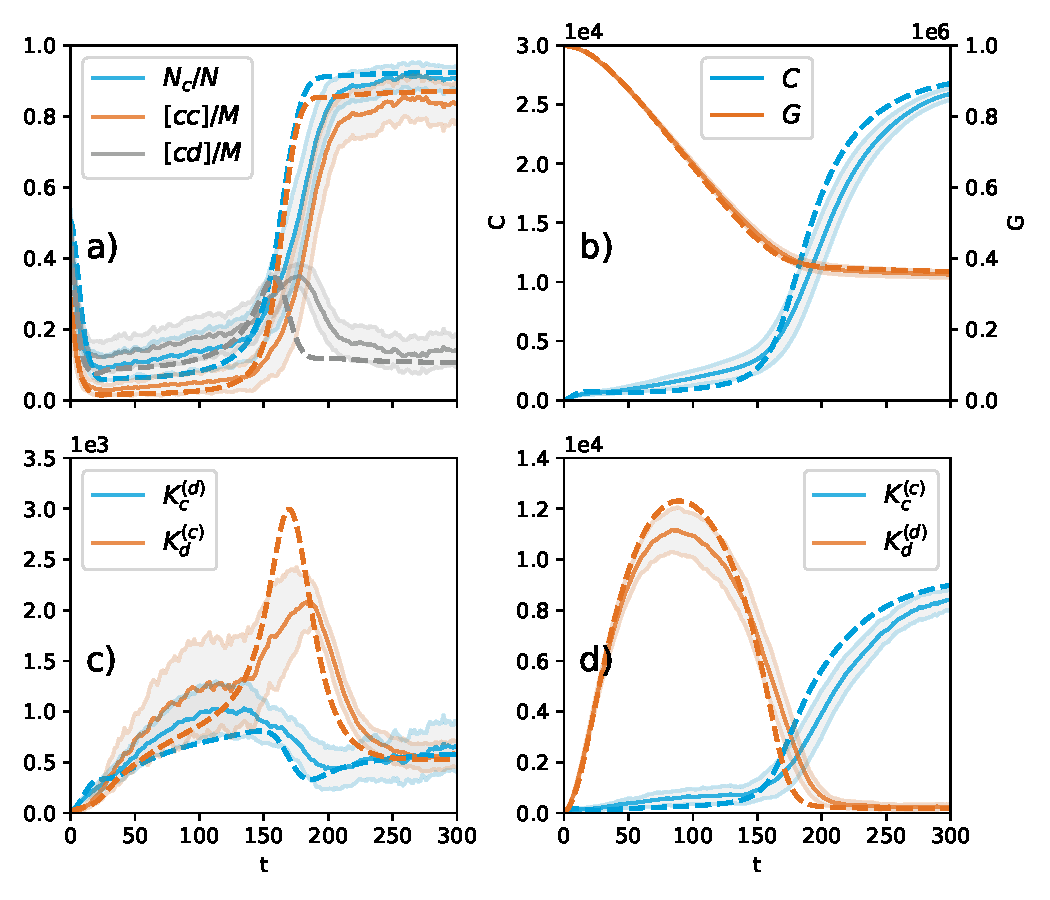
\includegraphics[width=.9\linewidth]{figures/micro_vs_approx_v2.pdf}
\caption{\textbf{Trajectories of dynamic variables from the macro approximation and from measurement in ABM simulations.} The results from ABM simulations (solid lines) are obtained as an ensemble average from 50 runs with standard errors indicated by gray areas. Initial conditions are given by equal shares of the $N=100$ households investing in both sectors and equal endowments in both sectors for all households. The initial acquaintance network amongst the households is an Erd\H{o}s-Renyi random graph with mean degree $k=10$. Other initial conditions are $C_0=0.5$ and $G_0=5 \times 10^5$. All other parameter are given in table \ref{tab:Parameter_list}. The results from the macro approximation (dashed lines of the same colors) are obtained by integration of the ODEs that are obtained from the large system limit with fixed per household quantities. The initial conditions are drawn from the same distribution as previously for the ABM simulations e.g. $N_c$, $[cc]$ and $[cd]$ are calculated from an Erd\H{o}s-Renyi random graph with mean degree $k=10$.}
\label{fig:comparison2}
\end{figure}
%\JK{Maybe better to structure the results as (1), (2), ... and do the same for the full model - then easier to compare}
The results in  fig.~\ref{fig:comparison2} are to some extent complementary to the results in fig.~\ref{fig:example_trajectory} that I discussed in section \ref{sec:numerical_results}. Fig.~\ref{fig:comparison2}d shows capital in both sectors belonging to households that actually invest in these sectors, which is almost equivalent to the variables in fig.~\ref{fig:example_trajectory}d as it makes up almost the entirety of these capital stocks. This can be seen in fig. \ref{fig:comparison2}c: It shows capital of households in the sector that they do not currently invest in, which is approximately an order of magnitude smaller (note the different scale of the y-axis in the figure).

A comparison of the results of the approximation (dashed lines) with those of the numerical simulation of the ABM (solid lines) in fig.~\ref{fig:comparison2} shows that the approximation exhibits the same qualitative features, such as trends, timing and order of magnitude of the displayed variables, as the microscopic model.

Particularly, these results show that for the given parameter values the macroscopic approximation is capable of reproducing very closely the quasi equilibrium states before and after the transition from the dirty to the clean sector, as it lies within the standard error of the ensemble of ABM runs. Also, the approximation is reasonably capable to reproduce the timing of and the transient states during the transition. This is somewhat surprising since in other works, macro-approximations were less well able to get the timing of transition right.

In the following, I discuss the existing differences between the results of the approximated model and the numerical simulation results. 

For instance, I find that the approximation estimates the transition from investment in the dirty sector to investment in the clean sector a bit too early (best visible in panel a). The reason for this might be the slight underestimation of the share of clean investing households, leading to a slight overestimation of the share of dirty capital in the system which is also visible in panel \ref{fig:comparison2}d.

I find a second obvious discrepancy between the micro-model and the approximation in the overestimation of dirty capital of clean investors ($K_d^{(c)}$) (panel c) during the transition phase between $t\approx 150$ and $t \approx 200$. This can be explained by the inequality in capital holdings amongst households. In the approximation, all households investing in dirty or clean capital are assumed to have the same income respectively. Therefore, the probability to change their investment behavior will change for all of them at once during the transition phase leading to a rapid shift of dirty investors changing to invest in clean capital but taking their dirty capital endowments with them (hence the sharp peak in dirty capital of clean investors during the transition phase, see fig.  \ref{fig:comparison2}c dashed grey line). 

Also, in the micro-model, households changing from a dirty to a clean investment strategy take their -- presumably high -- endowments in dirty capital with them. Therefore, the endowments in dirty capital of households investing in the clean sector are relatively wide-spread (see grey area around solid orange line in fig.~\ref{fig:comparison2}c. 
This has effects on the estimated timing of the transition, too. In the micro-model, income of households is heterogeneous. Therefore, for each of them the probability to change their investment behavior changes at different points in time, i.e., poorer households are likely to switch earlier during the transition than richer households. Together this leads to a slower, more spread-out transition dynamic the micro-model resulting in a flatter peak in the dirty capital endowments of clean-investing households.

Another effect at play during the transition is related to the assumptions in equations \ref{eq:neighbordist} and \ref{eq:additional_neighbors}. Namely, that all households that invest in the same type of capital have the same distribution of clean and dirty neighbors.

In the reality of the micro-model, however, these assumptions that are essential to the pair approximation may well be wrong -- especially so during a rapid transition. E.g., a household that has only recently changed its state has a neighborhood that is atypical for its group and adapts only slowly. Consequently, when many changes in the state of the system happen in a short time, a significant proportion of the population is not well described by the assumed approximate distribution.

A number of these effects that lead to discrepancies between the micro-model and the approximation can be mitigated by higher-order moment closure for the distribution of heterogeneous agent-properties or higher-order motif approximation of the network dynamic.

For instance, a higher-order moment closure approximation that tracks the variance and skewness of the distribution of capital endowments can also account for the likelihood of capital endowments of agents that switch their investment decision to be biased. This would presumably mitigate the overestimation of dirty capital of clean investors ($K_d^{(c)}$) during the transition as well as the underestimation of ($K_d^{(c)}$) before the transition and therefore also estimate the timing of the transition even more precisely. 

Similarly, a higher-order motif approximation of the network dynamic can describe the heterogeneity in the local distribution of opinions in the neighborhood of individual agents and correct for the effects of this especially during periods of transient non equilibrium dynamics in the approximated model.\\

In the previous section I derived a set of ordinary differential equations describing the stochastic dynamics of an agent-based model in terms of aggregated variables in the large system limit. I intend this derivation to be a prototypical example for a macroeconomic model with true microfoundations based on heterogeneous agents, given their microscopic interactions are of similar complexity. As such, it might also serve as a starting point for the application and development of similar models for other kinds of social dynamics. For example, an extension to continuous opinions requiring a Fokker-Planck-type description would follow naturally and would grant compatibility to a large body of models for social influence \citep[see ref.][pp. 988 f.]{Mueller-Hansen2017}.

\section{Bifurcation Analysis}
\label{sec:bifurcation-analysis}

The description of the model as a system of ordinary differential equations allows for the analytical analysis of emergent model properties such as multi stability, tipping and phase transitions. 
As a proof of concept application I subsequently show the results of a bifurcation analysis.

\subsection{Methods}
%What is bifurcation analysis?
Bifurcation theory is the analysis of qualitative changes of dynamical systems under parameter variation, for example between a regime with a unique equilibrium (fixed point) and a multi-stable regime.
The parameter value at which a qualitative change, for example in the stability of an equilibrium, occurs is called a critical value or bifurcation point. Bifurcations are classified according to the changes in dynamical properties of the system \cite{Strogatz1994,Kuznetsov1998}.
% Methods for Bifurcation Analysis
Analytical methods have limited scope to identify bifurcation points in non-linear systems. Methods like numerical continuation can handle complex systems of ordinary differential equations like the one derived in section \ref{sec:Approximation} \citep{Allgower2003}.
Consequently, I use numerical continuation from PyDSTool, a Python package for dynamical systems modeling and analysis \citep{pydstool,10.1371/journal.pcbi.1002628}.\footnote{PyDSTool is building on the AUTO-07p continuation library \citep{Doedel07auto-07p:continuation}.}

% Introduce those kinds of bifurcations that I observe in the analysis:
A common bifurcation type that appears in this model is the fold bifurcation that is also known as saddle-node bifurcation. This type is a local bifurcation in which a stable fixed point collides with an unstable one and both disappear. 
%\JK{Normal form ect. necessary here?} It is described by the normal form $\dot{x} = r + x^2$ with bifurcation parameter $r$. The bifurcation point at $r = 0$ divides a regime with two equilibria for $r < 0$ and a regime without any equilibria for $r > 0$.

Varying two bifurcation parameters at the same time can result in even richer qualitative changes of the dynamics. A prevalent example for such a bifurcation is the cusp geometry \citep[][p.\.397]{Kuznetsov1998}. A change of the second bifurcation parameter in this geometry beyond a certain value results in the so-called cusp catastrophe: the multi-stability of the system disappears for all values of the first bifurcation parameter. As I will show in the following, the macro-approximation of this model indeed exhibits a cusp bifurcation. 

\subsection{Discussion of Results}

\begin{figure}[ht!]
\centering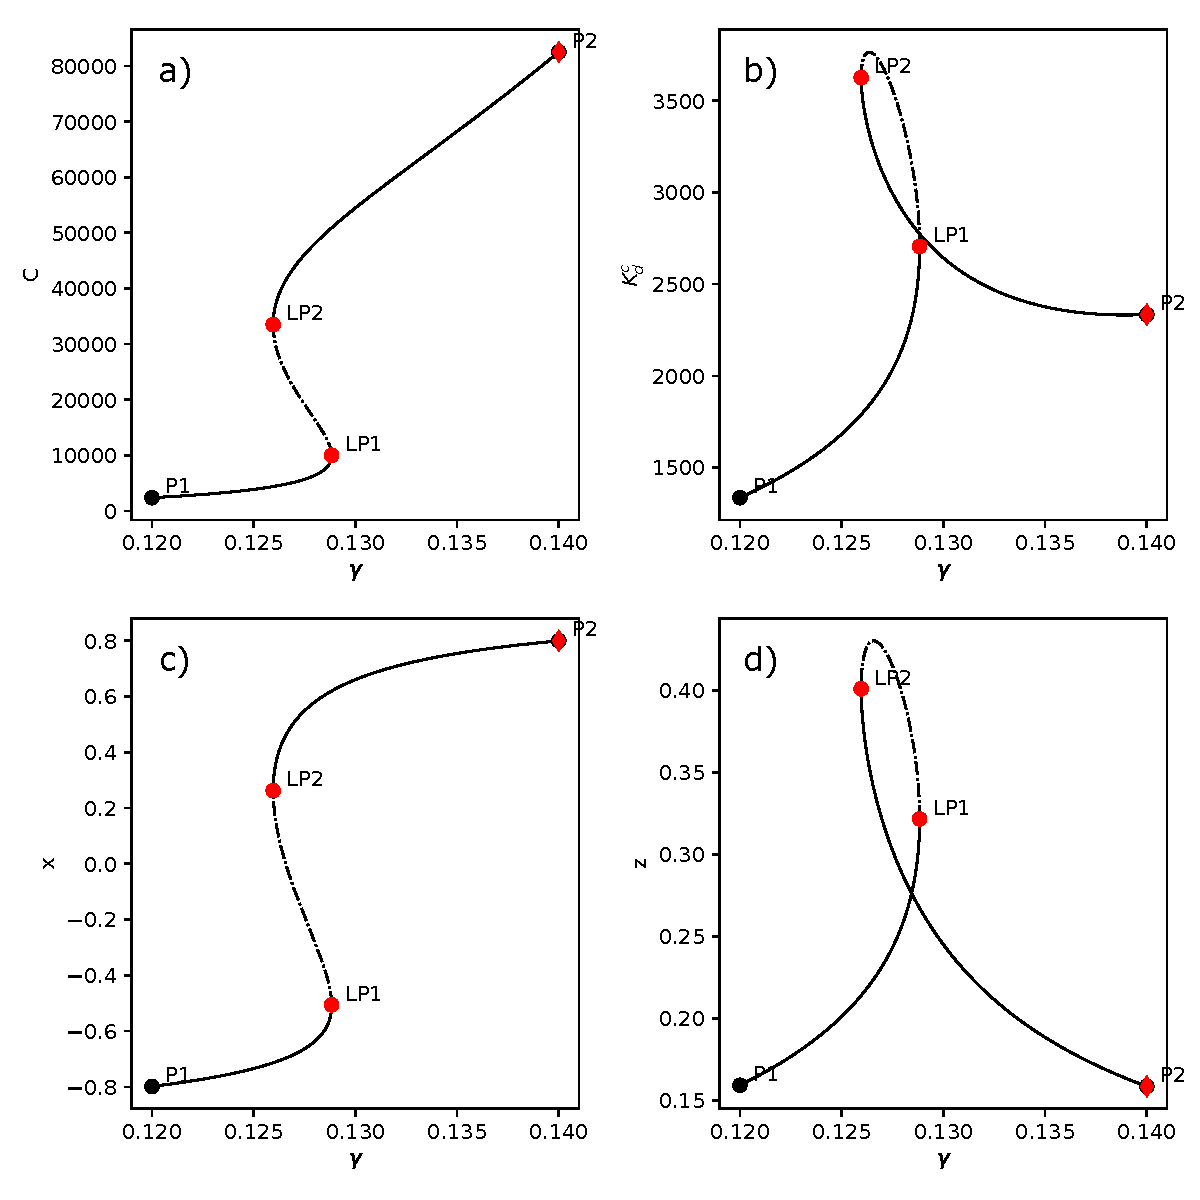
\includegraphics[width=.95\linewidth]{figures/ba_plot.pdf}
\caption{\textbf{Bifurcation diagram:} Continuation of the stationary solution of the macroscopic approximation without resource depletion, i.e. $\dot{G} = 0$ instead of the rate $R$ as given by eq. \eqref{eq:approx_surd}. Bifurcation parameter is $\gamma$, the elasticity of knowledge in the clean sector that also reflects the elasticity of learning by doing of the respective technology. The points labeled P1 and P2 are the beginning and end points of the continuation line, the points labeled LP1 and LP2 are the bifurcation points of two fold bifurcations. The stable unstable manyfold is indicated by a dotted line, the stable manyfold is indicated by solid line. Note that the intersections of the curves in the two right panels do not actually mean that the stationary manifold is not a bijective function of the bifurcation parameter $\gamma$ but rather a result of the projection of the multidimensional manifold onto the two dimensional space.\label{fig:bifurcation_analysis}}
\end{figure}

\begin{figure}[ht!]
\centering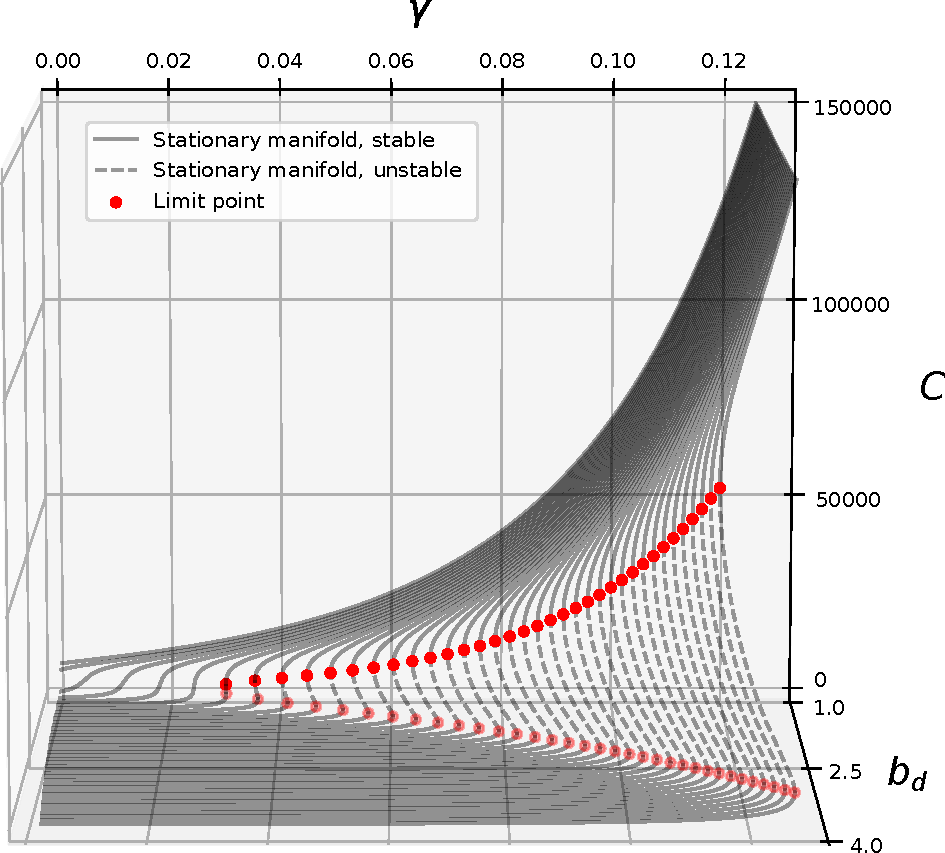
\includegraphics[width=\linewidth]{figures/cusp_better.pdf}
\caption{\textbf{Cusp Bifurcation diagram:}
Stationary manyfold from figure \ref{fig:bifurcation_analysis} panel a for different values of the total factor productivity on the dirty sector $b_d$. Red dots indicate the limit points of the one dimensional fold bifurcation separating the stable and the unstable parts of the stationary manyfold indicated by a solid and a dashed line respectively. For a critical value of $b_d \approx 1.4$ and $\gamma \approx 0.03034$ the two limit points converge and annihilate each other. This codimension two bifurcation with bifurcation parameters $\gamma$ and $b_d$ is called a cusp catastrophe. In this two-sector economic model, this results in a lock in effect in the dirty sector i.e. below this point, there is a smooth transition of production from the dirty to the clean sector and above this point production in the dirty sector is continued even though production in the clean sector would be more efficient. \label{fig:cusp}}
\end{figure}

A considerable advantage of the description of my model in terms of ordinary differential equations \eqref{eq:approx_surd}, \eqref{eq:sum_up_learning} \eqref{eq:lsl_transitions} and \eqref{eq:lsl_capital} over agent based modeling is the fact that it allows for the usage of established tools for bifurcation analysis.
As a proof of concept, I show some results in figure \ref{fig:bifurcation_analysis}.
Here, I analyze the possible steady states of the system with abundant fossil resources i.e. the possible equilibrium states of the model in the regime before the fossil resource becomes scarce and acts as an external driver on the system pushing it towards clean investment.
Therefore, I set the resource depletion to zero i.e. I keep the resource stock in eq. \eqref{eq:approx_surd} constant $G(t) \equiv G_0$ such that the resource usage cost $c_R$ still depends on resource use $R$ but is not increased by deceasing resource stock $G$. Thereby, I eliminate the rising resource extraction cost as the constraint in \cref{eq:approx_equilibrium_wage,eq:approx_dcr} that eventually halts production in the dirty sector. 
I chose the learning rate $\gamma$ as bifurcation parameter as I expect it to yield interesting results.
%That is because as an exponent to a dynamical variable it determines its growth pattern leading to subexponential, exponential or superexponential growth for different values \JK{CITATION NEEDED}. \FMH{I would drop the last sentence because this should be only relevant if I would also consider gamma > 1, but this is certainly not a valid parameter value}.
Generally, in nonlinear dynamical systems, exponential factors are expected to have a strong influence on dynamical properties. Therefore, changing these factors is expected to lead to bifurcation behavior.
Consequently, in figure \ref{fig:bifurcation_analysis} panel a and c I see that for certain learning rates $\gamma$ the macroscopic approximation exhibits a bistable regime limited by two fold bifurcations with bifurcation points indicated by LP1 and LP2.
In this regime both low investment in the clean sector together with hight investment in the dirty sector and low knowledge as well as high investment in the clean sector together with low investment in the dirty sector and high knowledge are stable states of the economic system. This means that in this region economic outcomes are highly path dependent i.e. starting with slightly different knowledge about clean technologies may lead to widely differing adoption levels of the technology in the long run.

Figure \ref{fig:cusp} shows an example of how this bifurcation structure of the dynamical system depends on other parameters. Varying the total factor productivity in the dirty sector $b_d$, the system undergoes a cusp bifurcation. Above a certain value of $b_d$ the system exhibits bi-stability whereas below this value it does not.

%\FMH{Add some words about possible extensions of this analysis?}

Clearly, this choice of bifurcation parameters is only one of many and other choice may very well lead to interesting results. However, I had to limit ourselves to this proof of concept study as an extensive analysis of all possible combinations would be well beyond the scope of this work.

%\FMH{Do I need this sentence?: Such a configuration would have profound implications on policy design to foster clean technology in order to drive a decarbonization transition in the models production economy.}

Multi-stability of the economy would mean that policies could make use of inherent dynamical properties of the system to reach a desired state or bring the system onto a desired pathway. For example, policy measures such as regulation or taxes can help driving the system into another basin of attraction, i.e. a region of the phase-space in which trajectories approach another equilibrium in the long term. To do so, the system has to cross a separatrix, the boundary between two basins of attraction.
After this boundary is crossed, the policy measure can be discontinued, the system's dynamics guarantee that it reaches the new equilibrium. 
Figure \ref{fig:cusp} shows that such an intervention could be complemented by an additional policy measure, lowering the total factor productivity in the dirty sector, effectively reducing the distance of the stable manyfold from the separatrix and thereby presumably making the first measure less costly.
Another possibility to take advantage of the system's inherent dynamical structure is to use its hysteresis, i.e. to find policy measures that change the first bifurcation parameter $\gamma$ across a bifurcation point or to change the second bifurcation parameter $b_d$ to move the bifurcation point past the current state of the system (or a combination of both) after which the system would fall to the other branch of the stable manyfold. Afterwards, the policy can be discontinued and the system would remain in its new state.
For such considerations, tools from dynamical systems theory and topology can be used to classify the phase-space of the system into regions with respect to the reachability of a desirable state \citep{Heitzig2016,Nitzbon2017}. This allows designing temporary policies that leverage the multi-stability of the socio-economic system.

\section{Discussion and Conclusion}
\label{sec:approx_conclusion}
% Summary: Method
This chapter combines a set of methods to overcome shortcomings of current approaches to base macroeconomic models on microfoundations.
While representative agent approaches are unable to capture dynamics that emerge from structured and local interactions of multiple heterogeneous agents, computational agent-based approaches have the disadvantage that they make tractable model analysis difficult and computationally challenging.
I demonstrated that a combination of approximation techniques allows finding a macro description of a multi-agent system in which heterogeneous agents interact locally on a complex adaptive network as well as via aggregated quantities. 
In contrast to previous analytic work, where the network structure was either static \cite{Lux2016}, restricted to star like clusters \cite{DiGuilmi2012} or approximated by a mean field interaction approach and hence neglected \cite{Aoki1998, Aoki2007, Alfarano2008a, DiGuilmi2008, Chiarella2011a}, I explicitly treat the structure of the adaptive complex interaction network with appropriate approximation methods.

I develop a stylized two-sector investment model, in which investment decisions are driven by a social imitation process, to showcase the three approximations:
First, a pair approximation of networked interactions takes into account the heterogeneity in interaction patterns.
Second, a moment closure approximation makes it possible to deal with heterogeneous attributes that characterize the agents.
Third, the large-system limit abstracts from effects due to finite population size.
It is only possible to take this limit if the model has at least one of the following properties: (i) individual interaction depend only on relative rather than absolute quantities such that the size of households can be decreased while taking the number of households to infinity or (ii) the economic production functions exhibits constant returns to scale such that they scale linearly with the number of households $N$.
The resulting set of ordinary differential equations captures the effect of local interactions at the system level while still allowing for analytical tractability.

% Summary: Results
A comparison between a computational version of the ABM and the macro-description reveals that the approximation works well for parameter values distinct from special cases even if only accounting for first moments. Taking more moments into account would increase accuracy but comes at the cost of higher dimensionality and complexity of the macroscopic dynamical system.

% Learnings from model dynamics (topic-wise)
This model shows that social imitation dynamics add inertia to the investment decisions in the system that cannot be captured by a representative agent approach.
The imitation process results in social learning such that agents tend to direct their investments into the more profitable sector over time.
Because of this, the shift of investments from the dirty (fossil) to the clean (renewable) sector is driven only by economic factors, namely increasing exploration and extraction costs for the fossil energy resource.
Thus, I conclude that neutral imitation of better performing peers is not a feasible mechanism to initiate a bottom-up transformation of the economy. Directed imitation, for example driven by changes in social norms, and supporting policies that make dirty production less profitable are needed to initiate a transformation towards a sustainable economy in the absence of fossil resource shortage.

% Why is analytical description desirable
Finding a system of ordinary differential equations to approximate ABMs is useful because it makes the analysis of the dynamical properties of the model much easier. One promising application here is bifurcation theory, as illustrated in section \ref{sec:bifurcation-analysis}.
Furthermore, it opens the possibility to mathematically proof model properties such as the dependency between different parameters and variables in the model.

% Outlook
% discuss further application 
In the context of climate economics and policy, the proposed techniques are especially important because they allow investigating the interplay of learning agents adapting to new policies and effects of shifts in values and preferences. The resulting changes in individual behavior and their impact on macroeconomic dynamics can be studied in a comprehensive modeling framework. 
Large shifts in investments that are required to reach the goals of the Paris agreement are likely to profit from both, policies that rely on price signals, as well as policies that target individual norm change, interaction and behavior not unlike those researched in e.g. the public health context \cite{Zhang2016, Zhang2015, Centola2011}. The presented techniques can help to better understand how such behavioral interventions would impact the macro-level dynamics of the economic system.

% more specific outlook
%On this regard, there are several promising avenues to develop the model and approximation techniques further: For example, instead of binary opinions, the social interaction model can use continuous variables to represent gradual opinions, drawing on a variety of models of social influence \citep[see ref.][pp. 988 f.]{Mueller-Hansen2017}. An approximation of the agent ensemble would then need a Fokker-Planck-type description rather than a master equation.

% economic modifications
% The model could be extended to explicitly include policy instruments such as a carbon tax and explore its impact on the investment decisions of the heterogeneous agent population. Another promising modification could include consumption decisions into this two-sector model. Consumption decisions are strongly influenced by social norms and interactions \citep{Peattie2010}. Their inclusion could inform the discussion about green consumption as a potential mechanism for a bottom-up transformation towards a more sustainable economy.

% Finally, the techniques proposed in this paper could be used to approximate other systems that interact both locally on a network and in an aggregate way on the system level, for example social-ecological systems or neural networks.
% cite here? \citep{Schlueter2012}


        \chapter{General Conclusion}

%        \chapter{Epilogue: Collective Knowledge Creation on Complex Contagion Phenomena}




        \appendix
 %       \addcontentsline{toc}{part}{Appendix}
 %       \part*{Appendix}
 %      \KOMAoptions{paper=a1}
\recalctypearea

Full system of equations resulting from the approximations in section \cref{sec:Approximation}:

\begin{align*}
  \dot{x} = &- \frac{1.0 \epsilon x}{\tau} + \frac{1.0 z \left(\epsilon - 1\right) \left(\phi - 1\right) \left(x - 1\right)}{\tau \left(y - 1\right) \left(e^{\frac{8.0 \left(W_{c} - W_{d}\right)}{W_{c} + W_{d}}} + 1\right)} - \frac{1.0 z \left(\epsilon - 1\right) \left(\phi - 1\right) \left(x + 1\right)}{\tau \left(1 + e^{- \frac{8.0 \left(W_{c} - W_{d}\right)}{W_{c} + W_{d}}}\right) \left(y + 1\right)} \\
%
  \dot{y} = &- \frac{1.0 \epsilon m y}{\tau} + \frac{1.0 m z \left(\epsilon - 1\right) \left(\phi - 1\right)}{\tau \left(e^{\frac{8.0 \left(W_{c} - W_{d}\right)}{W_{c} + W_{d}}} + 1\right)} - \frac{1.0 m z \left(\epsilon - 1\right) \left(\phi - 1\right)}{\tau \left(1 + e^{- \frac{8.0 \left(W_{c} - W_{d}\right)}{W_{c} + W_{d}}}\right)} \\
    & + \frac{\left(x - 1\right) \left(0.25 \epsilon z \left(x - 1\right) - 0.25 \epsilon \left(x + 1\right) \left(y + z - 1\right) + 0.5 \phi z \left(\epsilon - 1\right)\right)}{\tau \left(y - 1\right)} \\
    & + \frac{\left(x + 1\right) \left(0.25 \epsilon z \left(x + 1\right) + 0.25 \epsilon \left(x - 1\right) \left(y - z + 1\right) - 0.5 \phi z \left(\epsilon - 1\right)\right)}{\tau \left(y + 1\right)}\\
%
    \dot{z} = &- \frac{1.0 \epsilon m \left(2 z - 1\right)}{\tau} \\
    &- \frac{0.5 z \left(\epsilon - 1\right) \left(\phi - 1\right) \left(\left(x - 1\right) \left(y - 1\right) - 2 \left(y + 2 z - 1\right) \left(m y - m - 0.5 x + 0.5\right)\right)}{\tau \left(y - 1\right)^{2} \left(e^{\frac{8.0 \left(W_{c}-W_{d}\right)}{W_{c} + W_{d}}} + 1\right)} \\
    & - \frac{0.5 z \left(\epsilon - 1\right) \left(\phi - 1\right) \left(\left(x + 1\right) \left(y + 1\right) - 2 \left(y - 2 z + 1\right) \left(m y + m - 0.5 x - 0.5\right)\right)}{\tau \left(1 + e^{- \frac{8.0 \left(W_{c} - W_{d}\right)}{W_{c} + W_{d}}}\right) \left(y + 1\right)^{2}} \\
    & + \frac{\left(x - 1\right) \left(0.25 \epsilon z \left(x - 1\right) - 0.25 \epsilon \left(x + 1\right) \left(y + z - 1\right) + 0.5 \phi z \left(\epsilon - 1\right)\right)}{\tau \left(y - 1\right)} \\
    & - \frac{\left(x + 1\right) \left(0.25 \epsilon z \left(x + 1\right) + 0.25 \epsilon \left(x - 1\right) \left(y - z + 1\right) - 0.5 \phi z \left(\epsilon - 1\right)\right)}{\tau \left(y + 1\right)}
  \end{align*}
%

\begin{align*}
    \dot{C} = - C \delta + C^{\xi} b_{c} \left(\frac{L \left(C^{\xi} b_{c} \left(K^{(c)}_{c} + K^{(d)}_{c}\right)^{\kappa_{c}}\right)^{\frac{1.0}{1.0 - \pi}}}{\left(b_{d} \left(K^{(c)}_{d} + K^{(d)}_{d}\right)^{\kappa_{d}}\right)^{\frac{1.0}{1.0 - \pi}} \left(1.0 - \frac{G_{0}^{2} b_{R}}{G^{2} e}\right)^{\frac{1.0}{1.0 - \pi}} + \left(C^{\xi} b_{c} \left(K^{(c)}_{c} + K^{(d)}_{c}\right)^{\kappa_{c}}\right)^{\frac{1.0}{1.0 - \pi}}}\right)^{\pi} \left(K^{(c)}_{c} \left(\frac{x}{2} + \frac{1}{2}\right) + K^{(d)}_{c} \left(\frac{1}{2} - \frac{x}{2}\right)\right)^{\kappa_{c}}
\end{align*}
\begin{align*}
    \dot{G} = - \frac{L^{\pi} b_{d}}{e} \left(\frac{\left(b_{d} \left(K^{(c)}_{d} + K^{(d)}_{d}\right)^{\kappa_{d}}\right)^{\frac{1.0}{1.0 - \pi}} \left(1.0 - \frac{G_{0}^{2} b_{R}}{G^{2} e}\right)^{\frac{1.0}{1.0 - \pi}}}{\left(b_{d} \left(K^{(c)}_{d} + K^{(d)}_{d}\right)^{\kappa_{d}}\right)^{\frac{1.0}{1.0 - \pi}} \left(1.0 - \frac{G_{0}^{2} b_{R}}{G^{2} e}\right)^{\frac{1.0}{1.0 - \pi}} + \left(C^{\xi} b_{c} \left(K^{(c)}_{c} + K^{(d)}_{c}\right)^{\kappa_{c}}\right)^{\frac{1.0}{1.0 - \pi}}}\right)^{\pi} \left(K^{(c)}_{d} + K^{(d)}_{d}\right)^{\kappa_{d}}
\end{align*}
  \begin{align*}
    \dot{K}_c^{(c)}=& - \delta K^{(c)}_{c} \\
&+ \frac{K^{(c)}_{c} L^{\pi} \kappa_{c} s \left(C^{\xi} b_{c} \left(K^{(c)}_{c} + K^{(d)}_{c}\right)^{\kappa_{c}}\right)^{\frac{1.0}{1.0 - \pi}} \left(\left(b_{d} \left(K^{(c)}_{d} + K^{(d)}_{d}\right)^{\kappa_{d}}\right)^{\frac{1.0}{1.0 - \pi}} \left(1.0 - \frac{G_{0}^{2} b_{R}}{G^{2} e}\right)^{\frac{1.0}{1.0 - \pi}} + \left(C^{\xi} b_{c} \left(K^{(c)}_{c} + K^{(d)}_{c}\right)^{\kappa_{c}}\right)^{\frac{1.0}{1.0 - \pi}}\right)^{- \pi}}{K^{(c)}_{c} + K^{(d)}_{c}} \\
&+ \frac{K^{(c)}_{d} L^{\pi} \kappa_{d} s \left(b_{d} \left(K^{(c)}_{d} + K^{(d)}_{d}\right)^{\kappa_{d}}\right)^{\frac{1.0}{1.0 - \pi}} \left(1.0 - \frac{G_{0}^{2} b_{R}}{G^{2} e}\right)^{\frac{1.0}{1.0 - \pi}} \left(\left(b_{d} \left(K^{(c)}_{d} + K^{(d)}_{d}\right)^{\kappa_{d}}\right)^{\frac{1.0}{1.0 - \pi}} \left(1.0 - \frac{G_{0}^{2} b_{R}}{G^{2} e}\right)^{\frac{1.0}{1.0 - \pi}} + \left(C^{\xi} b_{c} \left(K^{(c)}_{c} + K^{(d)}_{c}\right)^{\kappa_{c}}\right)^{\frac{1.0}{1.0 - \pi}}\right)^{- \pi}}{K^{(c)}_{d} + K^{(d)}_{d}} \\
&+ L L^{\pi - 1.0} \pi s \left(\left(b_{d} \left(K^{(c)}_{d} + K^{(d)}_{d}\right)^{\kappa_{d}}\right)^{\frac{1.0}{1.0 - \pi}} \left(1.0 - \frac{G_{0}^{2} b_{R}}{G^{2} e}\right)^{\frac{1.0}{1.0 - \pi}} + \left(C^{\xi} b_{c} \left(K^{(c)}_{c} + K^{(d)}_{c}\right)^{\kappa_{c}}\right)^{\frac{1.0}{1.0 - \pi}}\right)^{1.0 - \pi} \\
&- \frac{1.0 K^{(c)}_{c} \left(x + 1\right) \left(0.25 \epsilon \left(1 + e^{- \frac{8.0 \left(W_{c} - W_{d}\right)}{W_{c} + W_{d}}}\right) \left(y + 1\right) + 0.5 z \left(\epsilon - 1\right) \left(\phi - 1\right)\right)}{\tau \left(1 + e^{- \frac{8.0 \left(W_{c} - W_{d}\right)}{W_{c} + W_{d}}}\right) \left(y + 1\right)} \\
&- \frac{1.0 K^{(d)}_{c} \left(x - 1\right) \left(0.25 \epsilon \left(y - 1\right) \left(e^{\frac{8.0 \left(W_{c} - W_{d}\right)}{W_{c} + W_{d}}} + 1\right) - 0.5 z \left(\epsilon - 1\right) \left(\phi - 1\right)\right)}{\tau \left(y - 1\right) \left(e^{\frac{8.0 \left(W_{c} - W_{d}\right)}{W_{c} + W_{d}}} + 1\right)}
%
\end{align*}
\begin{align*}
%
  \dot{K}_d^{(c)}=&- K^{(c)}_{d} \delta - \frac{1.0 K^{(c)}_{d} \left(x + 1\right) \left(0.25 \epsilon \left(1 + e^{- \frac{8.0 \left(W_{c} - W_{d}\right)}{W_{c} + W_{d}}}\right) \left(y + 1\right) + 0.5 z \left(\epsilon - 1\right) \left(\phi - 1\right)\right)}{\tau \left(1 + e^{- \frac{8.0 \left(W_{c} - W_{d}\right)}{W_{c} + W_{d}}}\right) \left(y + 1\right)} \\
&- \frac{1.0 K^{(d)}_{d} \left(x - 1\right) \left(0.25 \epsilon \left(y - 1\right) \left(e^{\frac{8.0 \left(W_{c} - W_{d}\right)}{W_{c} + W_{d}}} + 1\right) - 0.5 z \left(\epsilon - 1\right) \left(\phi - 1\right)\right)}{\tau \left(y - 1\right) \left(e^{\frac{8.0 \left(W_{c} - W_{d}\right)}{W_{c} + W_{d}}} + 1\right)}\\
%
\dot{K}_c^{(d)}=& - K^{(d)}_{c} \delta +\frac{1.0 K^{(c)}_{c} \left(x + 1\right) \left(0.25 \epsilon \left(y + 1\right) \left(e^{\frac{8.0 \left(- W_{c} + W_{d}\right)}{W_{c} + W_{d}}} + 1\right) + 0.5 z \left(\epsilon - 1\right) \left(\phi - 1\right)\right)}{\tau \left(y + 1\right) \left(e^{\frac{8.0 \left(- W_{c} + W_{d}\right)}{W_{c} + W_{d}}} + 1\right)} \\
&+ \frac{1.0 K^{(d)}_{c} \left(x - 1\right) \left(0.25 \epsilon \left(y - 1\right) \left(e^{\frac{8.0 \left(W_{c} - W_{d}\right)}{W_{c} + W_{d}}} + 1\right) - 0.5 z \left(\epsilon - 1\right) \left(\phi - 1\right)\right)}{\tau \left(y - 1\right) \left(e^{\frac{8.0 \left(W_{c} - W_{d}\right)}{W_{c} + W_{d}}} + 1\right)}
\end{align*}
\begin{align*}
  \dot{K}_d^{(d)} =& - \delta K^{(d)}_{d} \\
    &+ \frac{K^{(d)}_{d} L^{\pi} \kappa_{d} s \left(b_{d} \left(K^{(c)}_{d} + K^{(d)}_{d}\right)^{\kappa_{d}}\right)^{\frac{1.0}{1.0 - \pi}} \left(1.0 - \frac{G_{0}^{2} b_{R}}{G^{2} e}\right)^{\frac{1.0}{1.0 - \pi}} \left(\left(b_{d} \left(K^{(c)}_{d} + K^{(d)}_{d}\right)^{\kappa_{d}}\right)^{\frac{1.0}{1.0 - \pi}} \left(1.0 - \frac{G_{0}^{2} b_{R}}{G^{2} e}\right)^{\frac{1.0}{1.0 - \pi}} + \left(C^{\xi} b_{c} \left(K^{(c)}_{c} + K^{(d)}_{c}\right)^{\kappa_{c}}\right)^{\frac{1.0}{1.0 - \pi}}\right)^{- \pi}}{K^{(c)}_{d} + K^{(d)}_{d}} \\
    &+ \frac{K^{(d)}_{c} L^{\pi} \kappa_{c} s \left(C^{\xi} b_{c} \left(K^{(c)}_{c} + K^{(d)}_{c}\right)^{\kappa_{c}}\right)^{\frac{1.0}{1.0 - \pi}} \left(\left(b_{d} \left(K^{(c)}_{d} + K^{(d)}_{d}\right)^{\kappa_{d}}\right)^{\frac{1.0}{1.0 - \pi}} \left(1.0 - \frac{G_{0}^{2} b_{R}}{G^{2} e}\right)^{\frac{1.0}{1.0 - \pi}} + \left(C^{\xi} b_{c} \left(K^{(c)}_{c} + K^{(d)}_{c}\right)^{\kappa_{c}}\right)^{\frac{1.0}{1.0 - \pi}}\right)^{- \pi}}{K^{(c)}_{c} + K^{(d)}_{c}} \\
    &+ L L^{\pi - 1.0} \pi s \left(\left(b_{d} \left(K^{(c)}_{d} + K^{(d)}_{d}\right)^{\kappa_{d}}\right)^{\frac{1.0}{1.0 - \pi}} \left(1.0 - \frac{G_{0}^{2} b_{R}}{G^{2} e}\right)^{\frac{1.0}{1.0 - \pi}} + \left(C^{\xi} b_{c} \left(K^{(c)}_{c} + K^{(d)}_{c}\right)^{\kappa_{c}}\right)^{\frac{1.0}{1.0 - \pi}}\right)^{1.0 - \pi} \\
    &+ \frac{1.0 K^{(c)}_{d} \left(x + 1\right) \left(0.25 \epsilon \left(y + 1\right) \left(e^{\frac{8.0 \left(- W_{c} + W_{d}\right)}{W_{c} + W_{d}}} + 1\right) + 0.5 z \left(\epsilon - 1\right) \left(\phi - 1\right)\right)}{\tau \left(y + 1\right) \left(e^{\frac{8.0 \left(- W_{c} + W_{d}\right)}{W_{c} + W_{d}}} + 1\right)} \\
    &+ \frac{1.0 K^{(d)}_{d} \left(x - 1\right) \left(0.25 \epsilon \left(y - 1\right) \left(e^{\frac{8.0 \left(W_{c} - W_{d}\right)}{W_{c} + W_{d}}} + 1\right) - 0.5 z \left(\epsilon - 1\right) \left(\phi - 1\right)\right)}{\tau \left(y - 1\right) \left(e^{\frac{8.0 \left(W_{c} - W_{d}\right)}{W_{c} + W_{d}}} + 1\right)}
\end{align*}

Where $W_d$ and $W_c$ are given by:
\begin{align*}
%
  W_c =& \frac{K^{c}_{c} L^{\pi} \kappa_{c} \left(C^{\xi} b_{c} \left(K^{c}_{c} + K^{d}_{c}\right)^{\kappa_{c}}\right)^{\frac{1.0}{1.0 - \pi}} \left(C^{\frac{1.0 \xi}{1.0 - \pi}} b_{c}^{\frac{1.0}{1.0 - \pi}} \left(K^{c}_{c} + K^{d}_{c}\right)^{\frac{1.0 \kappa_{c}}{1.0 - \pi}} + \left(b_{d} \left(K^{c}_{d} + K^{d}_{d}\right)^{\kappa_{d}}\right)^{\frac{1.0}{1.0 - \pi}} \left(1.0 - \frac{G_{0}^{2} b_{R}}{G^{2} e}\right)^{\frac{1.0}{1.0 - \pi}}\right)^{- \pi}}{K^{c}_{c} + K^{d}_{c}} \\
  &+ \frac{K^{c}_{d} L^{\pi} \kappa_{d} \left(b_{d} \left(K^{c}_{d} + K^{d}_{d}\right)^{\kappa_{d}}\right)^{\frac{1.0}{1.0 - \pi}} \left(1.0 - \frac{G_{0}^{2} b_{R}}{G^{2} e}\right)^{\frac{1.0}{1.0 - \pi}} \left(C^{\frac{1.0 \xi}{1.0 - \pi}} b_{c}^{\frac{1.0}{1.0 - \pi}} \left(K^{c}_{c} + K^{d}_{c}\right)^{\frac{1.0 \kappa_{c}}{1.0 - \pi}} + \left(b_{d} \left(K^{c}_{d} + K^{d}_{d}\right)^{\kappa_{d}}\right)^{\frac{1.0}{1.0 - \pi}} \left(1.0 - \frac{G_{0}^{2} b_{R}}{G^{2} e}\right)^{\frac{1.0}{1.0 - \pi}}\right)^{- \pi}}{K^{c}_{d} + K^{d}_{d}}, \\
%
  W_d =& \frac{K^{d}_{c} L^{\pi} \kappa_{c} \left(C^{\xi} b_{c} \left(K^{c}_{c} + K^{d}_{c}\right)^{\kappa_{c}}\right)^{\frac{1.0}{1.0 - \pi}} \left(C^{\frac{1.0 \xi}{1.0 - \pi}} b_{c}^{\frac{1.0}{1.0 - \pi}} \left(K^{c}_{c} + K^{d}_{c}\right)^{\frac{1.0 \kappa_{c}}{1.0 - \pi}} + \left(b_{d} \left(K^{c}_{d} + K^{d}_{d}\right)^{\kappa_{d}}\right)^{\frac{1.0}{1.0 - \pi}} \left(1.0 - \frac{G_{0}^{2} b_{R}}{G^{2} e}\right)^{\frac{1.0}{1.0 - \pi}}\right)^{- \pi}}{K^{c}_{c} + K^{d}_{c}}\\
  &+ \frac{K^{d}_{d} L^{\pi} \kappa_{d} \left(b_{d} \left(K^{c}_{d} + K^{d}_{d}\right)^{\kappa_{d}}\right)^{\frac{1.0}{1.0 - \pi}} \left(1.0 - \frac{G_{0}^{2} b_{R}}{G^{2} e}\right)^{\frac{1.0}{1.0 - \pi}} \left(C^{\frac{1.0 \xi}{1.0 - \pi}} b_{c}^{\frac{1.0}{1.0 - \pi}} \left(K^{c}_{c} + K^{d}_{c}\right)^{\frac{1.0 \kappa_{c}}{1.0 - \pi}} + \left(b_{d} \left(K^{c}_{d} + K^{d}_{d}\right)^{\kappa_{d}}\right)^{\frac{1.0}{1.0 - \pi}} \left(1.0 - \frac{G_{0}^{2} b_{R}}{G^{2} e}\right)^{\frac{1.0}{1.0 - \pi}}\right)^{- \pi}}{K^{c}_{d} + K^{d}_{d}}.
\end{align*}

\KOMAoptions{paper=a4}
\recalctypearea


        %\nocite{*}
		% See the documentation or under
		% http://edoc.hu-berlin.de/e_autoren/latex/bedingung.php
		% for the list of the permitted styles.
    \backmatter
    \bibliographystyle{plainnat}
    \bibliography{library.bib}
	%\printbibliography % biblatex bibliography
        %\printindex
        \selectlanguage{ngerman}

% You can change this text, if needed.
\chapter*{Selbst"andigkeitserkl"arung}

Ich erkl"are, dass ich die vorliegende Arbeit selbst"andig und nur unter Verwendung der angegebenen Literatur und Hilfsmittel angefertigt habe.

\vspace{2\baselineskip}
\noindent Potsdam, den \today \hfill\authorfirstname \authorsurname    % Use our template or write your own.
\end{document}
